\documentclass{../course_template/lectureClass}
%\usepackage{hyperref}
%\usepackage{svg}
%\usepackage{amsmath} % you need amsmath as the demo includes a use of \eqref
\makeglossaries
\begin{document}

%%%%%%%%%%%%%%%%%%%%%%%%%%%%%%%%%%%%%%%%%%%%%%%%%%%%%%%%%%%%%
%% Cover slide %%
%%%%%%%%%%%%%%%%%%%%%%%%%%%%%%%%%%%%%%%%%%%%%%%%%%%%%%%%%%%%%

\title[Power Electronics Devices]{Power Electronics Devices \\ (and Components)}
\author{Dr Bikash Sah}
\date{}
\begin{frame}[plain]
    \titlepage
\end{frame}

%%%%%%%%%%%%%%%%%%%%%%%%%%%%%%%%%%%%%%%%%%%%%%%%%%%%%%%%%%%%%
%% Outline / table of content %%
%%%%%%%%%%%%%%%%%%%%%%%%%%%%%%%%%%%%%%%%%%%%%%%%%%%%%%%%%%%%%
\begin{frame}{Content}
    \tableofcontents
\end{frame}

%%%%%%%%%%%%%%%%%%%%%%%%%%%%%%%%%%%%%%%%%%%%%%%%%%%%%%%%%%%%%
%% Lecture sections %%
%%%%%%%%%%%%%%%%%%%%%%%%%%%%%%%%%%%%%%%%%%%%%%%%%%%%%%%%%%%%%

%\includeonly{tex/Lecture01} % build only the specified file
%

\section{An initial overview of of the course}
\title[Initial overview]{Power Electronics Devices and Components}
 
\begin{frame}[plain]
    \titlepage
\end{frame}
%%%%%%%%%%%%%%%%%%%%%%%%%%%%%%%%%%%%%%%%%%%%%%%%%%%%%%%%%%%%%
%% Overview of the course %%
%%%%%%%%%%%%%%%%%%%%%%%%%%%%%%%%%%%%%%%%%%%%%%%%%%%%%%%%%%%%%
\begin{frame}
	\frametitle{Course Overview}
The course will be in 6 modules.
		\begin{itemize}
		  \item Module I: Basics of Electronics Devices.
		  \item Module II: Towards Power Semiconductor Devices- Introduction.
		  \item Module III: Conventional Power Semiconductor Devices.
		  \item Module IV: Next Generation Power Semiconductor Devices.
		  \item Module V: Passive Components.
		  \item Module VI: Way forward- Power Modules, Reliability, and Thermal Management
		\end{itemize}
\textbf{Pattern of class}: \\ Day: Thursday, every week \\ 
Time: 4 pm to 6 pm (theory) and 6 pm to 8 pm (tutorial) (ideally but it can change) \\
Holidays: 1st May, 29 May, and 19 June 2025. As required classes will be rescheduled. 
\end{frame}

%%%%%%%%%%%%%%%%%%%%%%%%%%%%%%%%%%%%%%%%%%%%%%%%%%%%%%%%%%%%%
%% Teaching Support Team %%
%%%%%%%%%%%%%%%%%%%%%%%%%%%%%%%%%%%%%%%%%%%%%%%%%%%%%%%%%%%%%
\begin{frame}
	\frametitle{The teaching team}
	\vspace{-0.5cm}
	\begin{columns}[t]
\centering
		\column[T]{0.5\textwidth}
		\begin{figure}
			\centering
				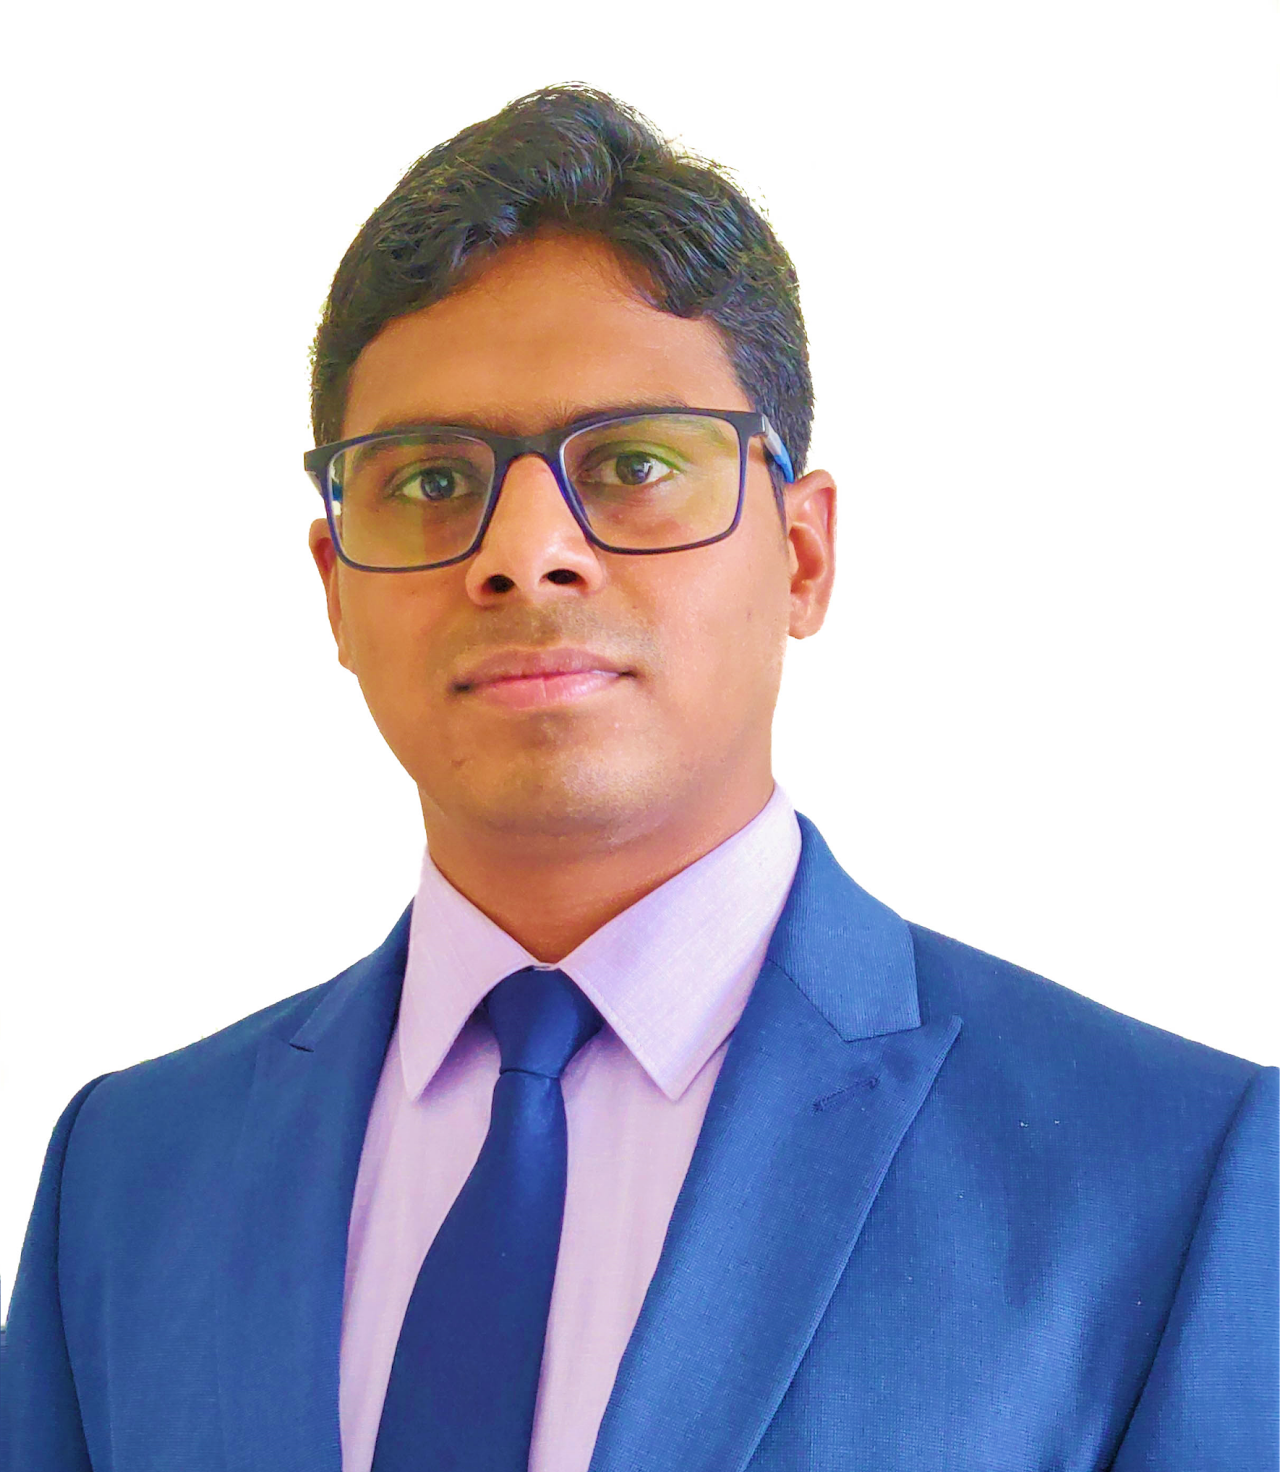
\includegraphics[height=2.5cm]{fig/lec01/Bikash.png}
				\caption*{Bikash Sah}
		\end{figure}
	
		\column[T]{0.5\textwidth}
		\begin{figure}
			\centering
				\includegraphics[height=2.5cm]{fig/lec01/ASack.jpg}
				\caption*{Andreas Sack}
		\end{figure}		
	\end{columns}
	\vspace{-0.5cm}
	\begin{varblock}{Contact}
		\begin{itemize}
			\item Email: see \href{https://www.eti.uni-siegen.de/ias/}{chair's homepage}
			\item Offices: H-A building, 4th floor
			\item Individual appointments on request (remote or personally)
            \item Multiple relevant courses are offered by the Chair.  \href{https://www.eti.uni-siegen.de/ias/teaching/}{Check link!}
		\end{itemize}
	\end{varblock}
** \small{Future follow-up courses are planned to be introduced in next semester- High Frequency Power Electronics, etc.}
	\end{frame}



%%%%%%%%%%%%%%%%%%%%%%%%%%%%%%%%%%%%%%%%%%%%%%%%%%%%%%%%%%%%%
%% Start %%
%%%%%%%%%%%%%%%%%%%%%%%%%%%%%%%%%%%%%%%%%%%%%%%%%%%%%%%%%%%%%
\begin{frame}
\center
\textbf{\huge{Module I: Basics of Electronics Devices}}
\end{frame}

%%%%%%%%%%%%%%%%%%%%%%%%%%%%%%%%%%%%%%%%%%%%%%%%%%%%%%%%%%%%%
%% What is Electronics %%
%%%%%%%%%%%%%%%%%%%%%%%%%%%%%%%%%%%%%%%%%%%%%%%%%%%%%%%%%%%%%
\begin{frame}
	\frametitle{What are "Electronic Devices"?}
	\begin{columns}
		\begin{column}{0.5\textwidth}
			\begin{varblock}{Electronic Devices}
				Electronic devices are hardware components which leverage the property of materials to control the flow of electrons or charge.
			\end{varblock} \vspace{-0.5cm}		
			\begin{itemize}
				\item<2-> Have a long history of development- started with the invention of vaccum tube or Thermionic valve in 1904 by J.A. Fleming.
				\item<3-> The first transistor was invented in 1947 by J.Bardeen, W.H. Brattain and W.S. Shockley in Bell Labs.
				\item<4-> The first integrated circuit was invented in 1958 by J. Kilby and R. Noyce -- On and it goes
%				\item<5-> The first microprocessor was invented in 1971 by F. Faggin, T. Klein and H. Hoff in Intel.
%				\item<6-> The first microcontroller was invented in 1971 by F. Faggin, T. Klein and H. Hoff in Intel.
%				\item<7-> On and it goes- every day new devices are invented and developed.
			\end{itemize}
		\end{column}
		\begin{column}{0.5\textwidth}
			\begin{figure}
				\centering
				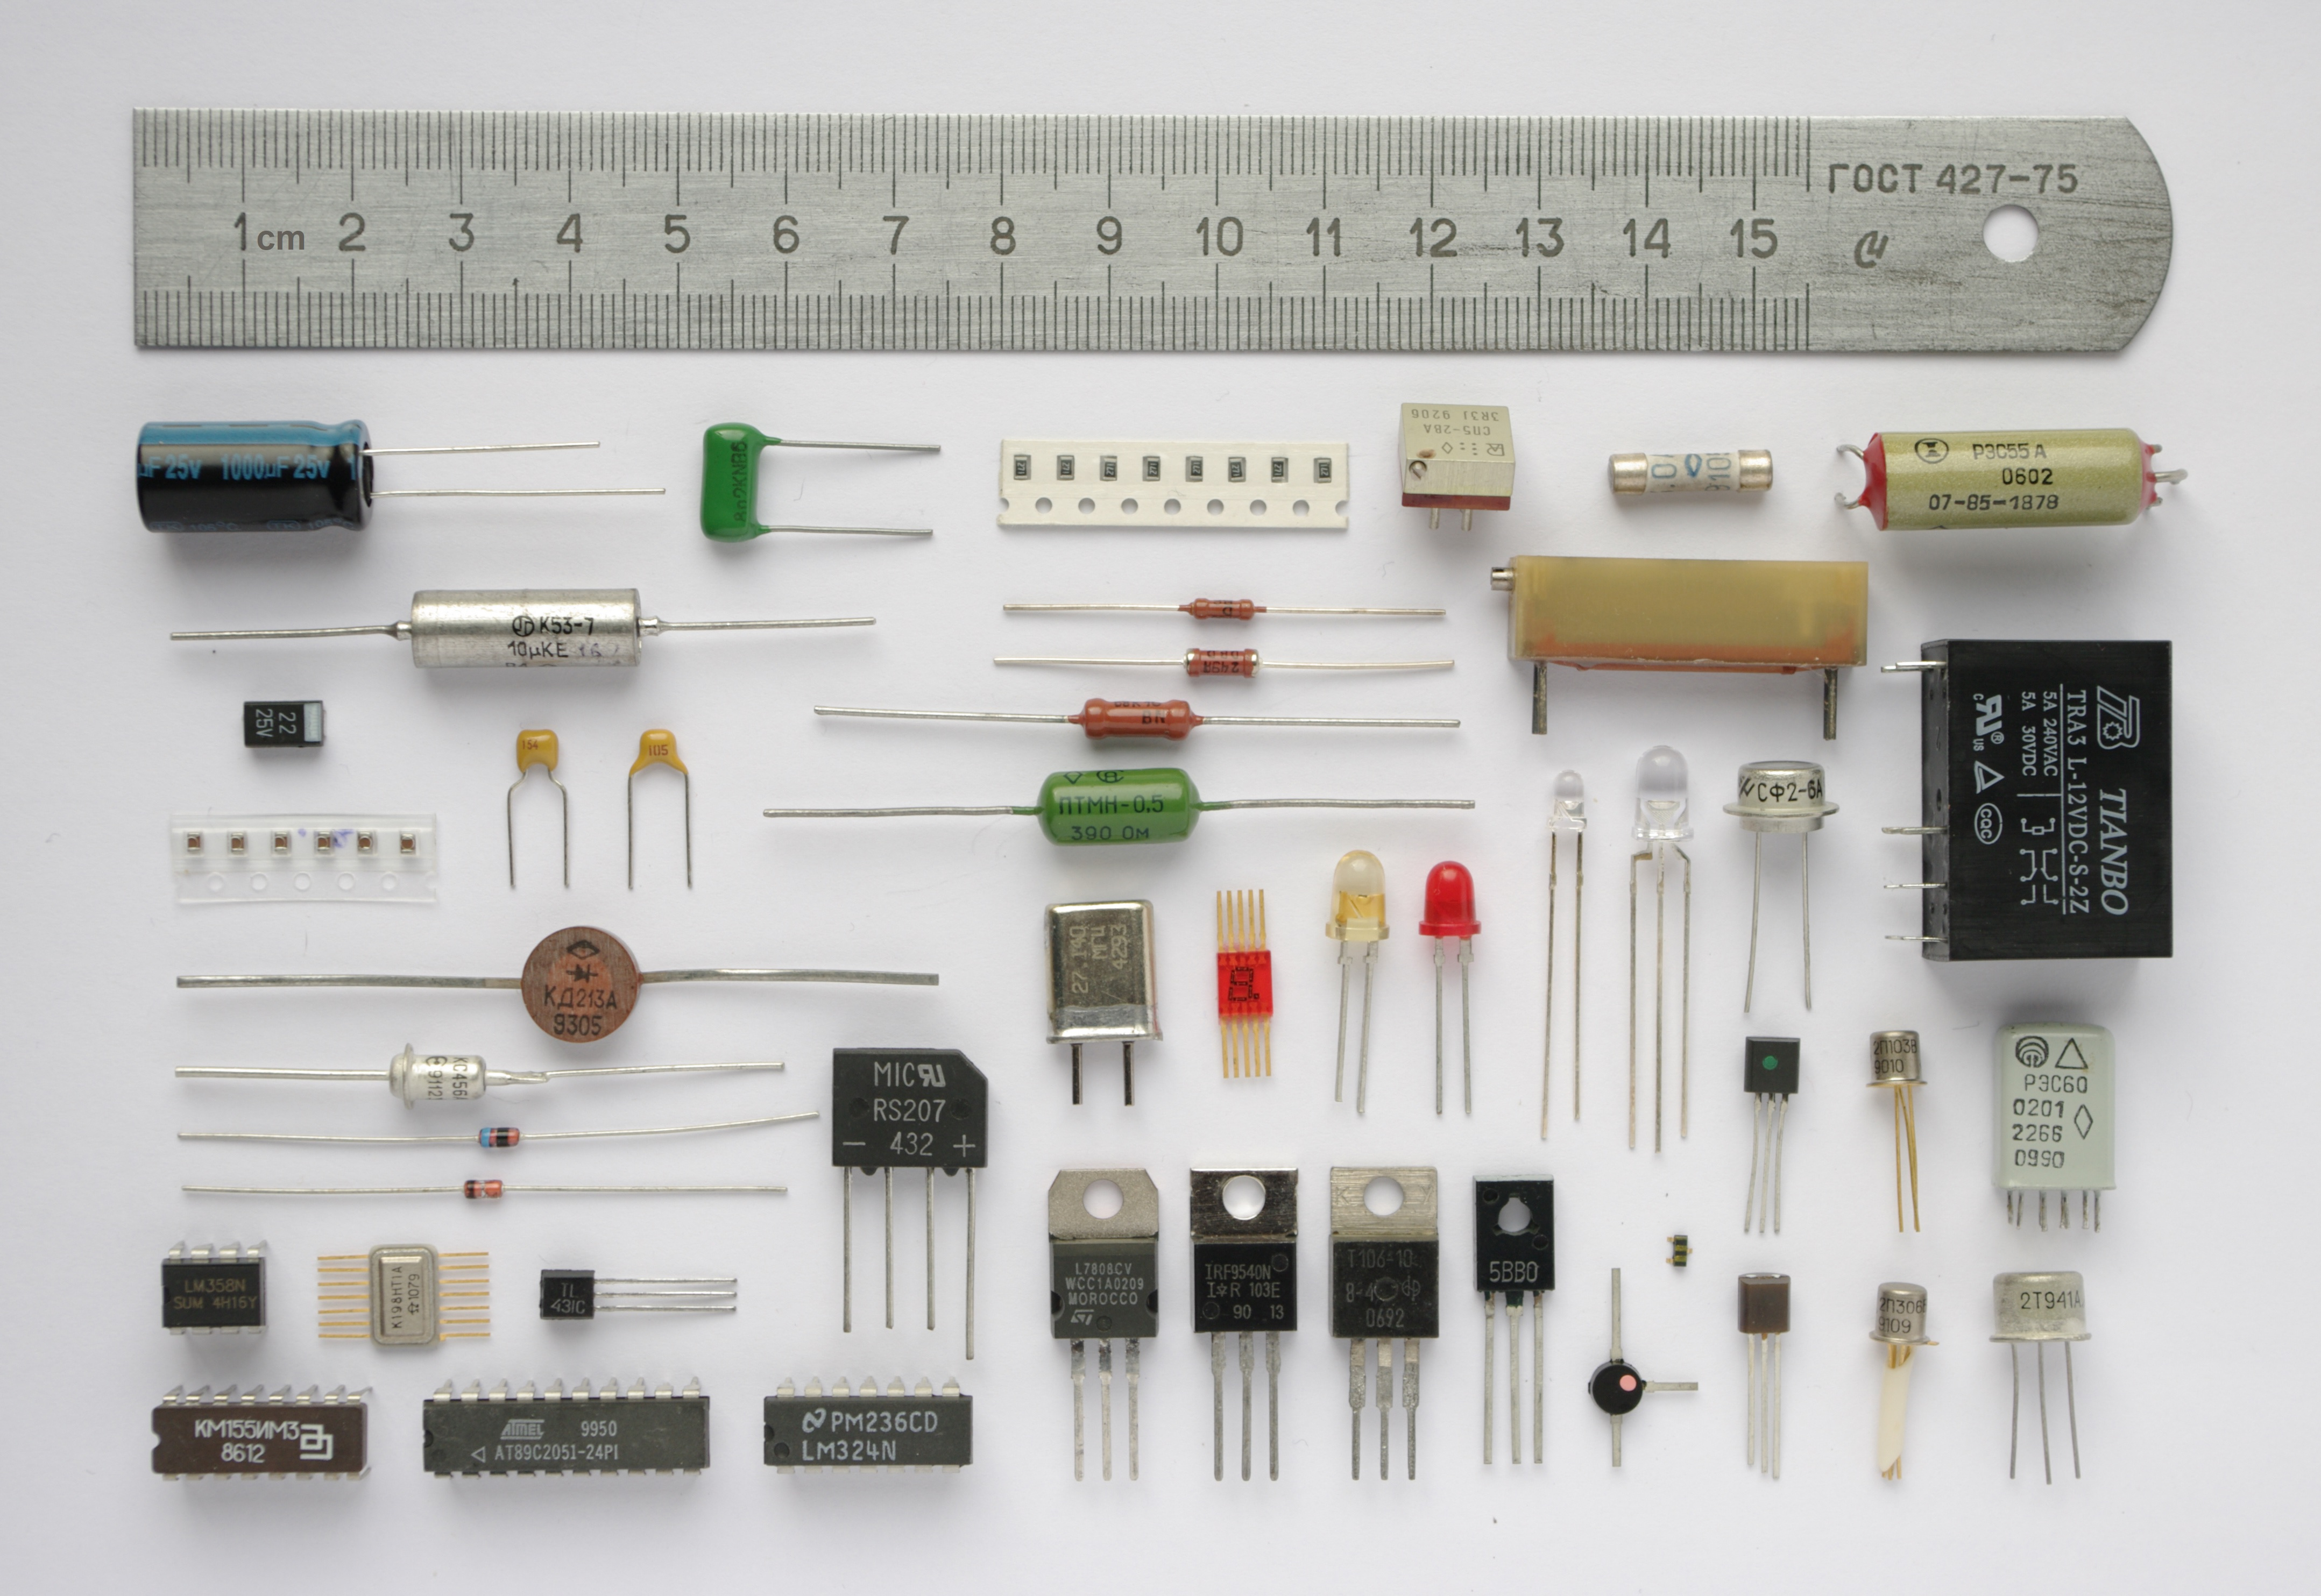
\includegraphics[scale= 0.05]{fig/lec01/Componentes.jpg}
				\caption{Example of electronic components (source: \href{https://commons.wikimedia.org/wiki/File:Componentes.JPG}{Wikimedia Commons}, Kae, public domain)}
			\end{figure}
		\end{column}
		\end{columns}
\end{frame}

%%%%%%%%%%%%%%%%%%%%%%%%%%%%%%%%%%%%%%%%%%%%%%%%%%%%%%%%%%%%%
%% Classification of electronics? %%
%%%%%%%%%%%%%%%%%%%%%%%%%%%%%%%%%%%%%%%%%%%%%%%%%%%%%%%%%%%%%
\begin{frame}
	\frametitle{General classification of "Electronic Devices"?}
	\begin{columns}
		\begin{column}{0.5\textwidth}

			\begin{itemize}
				\item<2-> Active devices: These are the devices which can control the flow of current and mainly consists of \textbf{semiconductor} materials. Examples: Transistor, Diode, etc.
				\item<3-> Passive devices: These are the devices which cannot control the flow of current and perform operation lke consuming, storing, or releasing power. Examples: Resistor, Capacitor, Inductor, etc.
			\end{itemize}
		\end{column}
		\begin{column}{0.5\textwidth}
			\begin{figure}
				\centering
				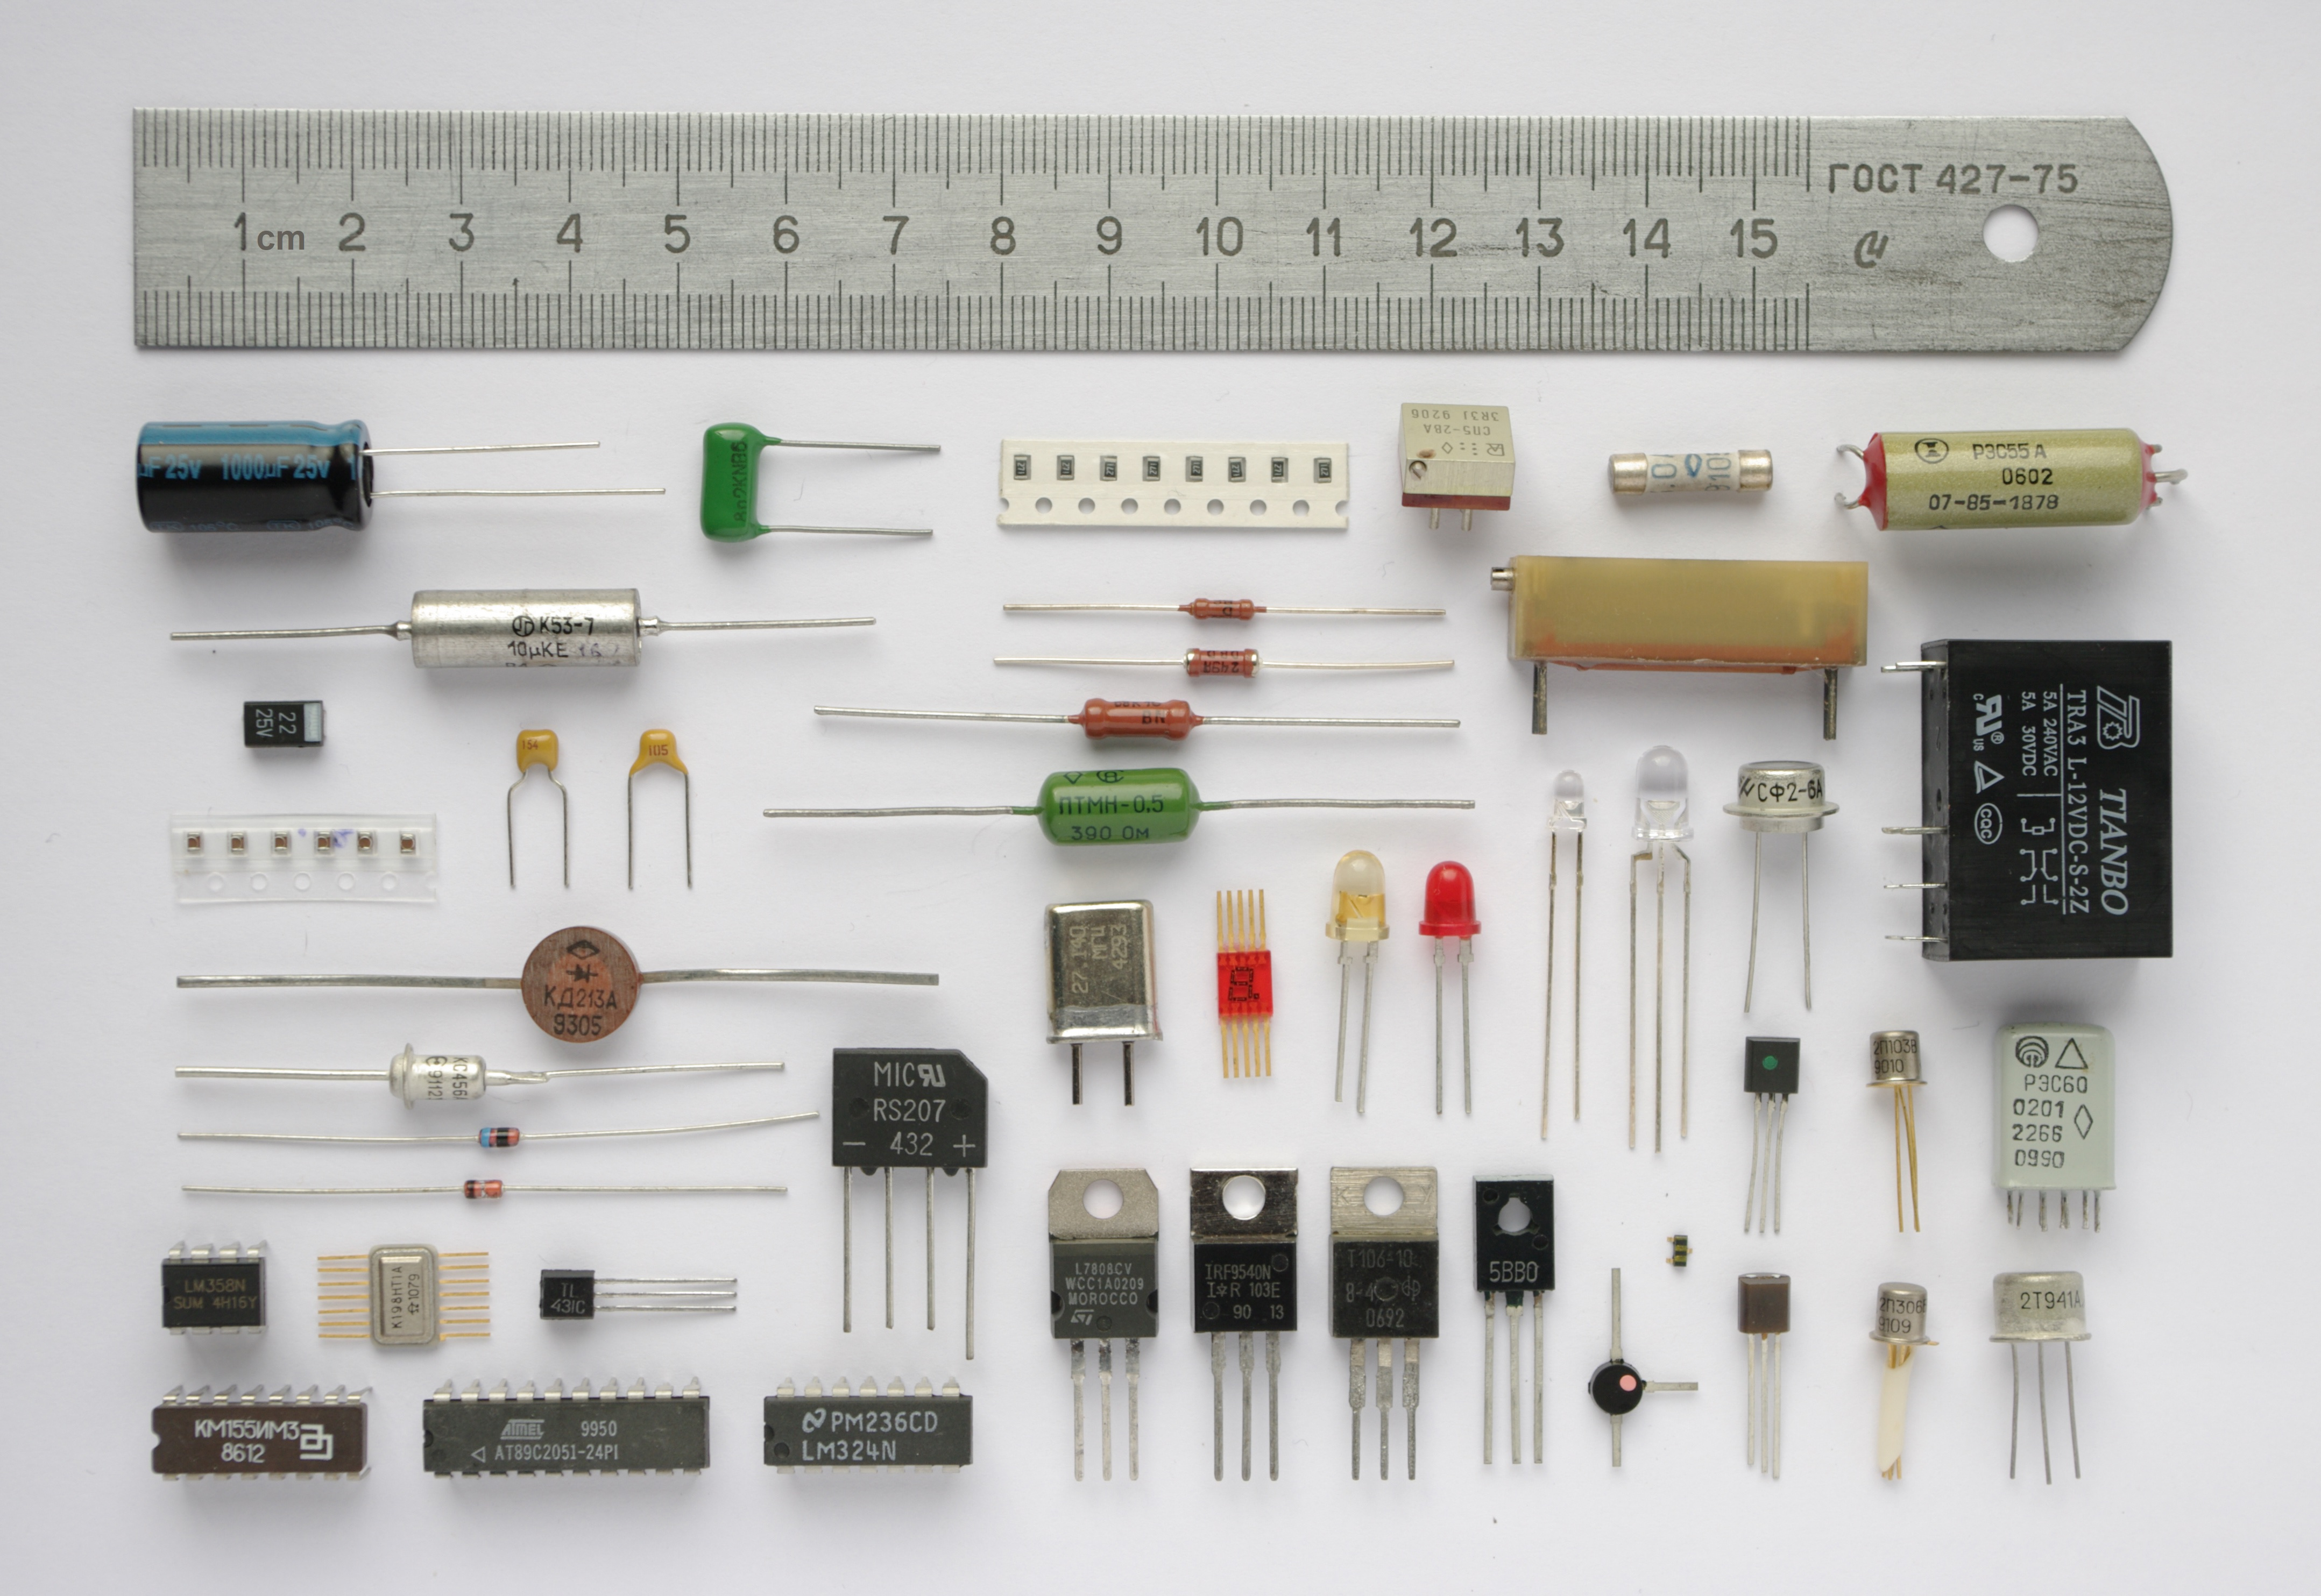
\includegraphics[scale= 0.05]{fig/lec01/Componentes.jpg}
				\caption{Example of electronic components (source: \href{https://commons.wikimedia.org/wiki/File:Componentes.JPG}{Wikimedia Commons}, Kae, public domain)}
			\end{figure}
		\end{column}
		\end{columns}
\end{frame}

%%%%%%%%%%%%%%%%%%%%%%%%%%%%%%%%%%%%%%%%%%%%%%%%%%%%%%%%%%%%%
%% Towards power electronics- difference between electroics and power electronics %%
%%%%%%%%%%%%%%%%%%%%%%%%%%%%%%%%%%%%%%%%%%%%%%%%%%%%%%%%%%%%%
\begin{frame}
	\frametitle{Comparison of Electronics and Power Electronics}
	\begin{table}[htbp] \small
		\centering
		\caption{Comparison between Electronics and Power Electronics} \footnotesize
		\begin{tabular}{|p{2.5cm}|p{4cm}|p{5cm}|}
		\hline
		\textbf{Feature} & \textbf{Electronics} & \textbf{Power Electronics} \\
		\hline
		\textbf{Primary Focus} & Signal processing, computation, communication & Energy conversion, control, and delivery \\
		\hline
		\textbf{Power Levels} & $\mu$W to a few watts & Tens of watts to megawatts \\
		\hline
		\textbf{Speed} & High-speed logic, RF, GHz range & Lower switching frequency (kHz–MHz), but high voltage/current \\
		\hline
		\textbf{Core Devices} & BJTs, MOSFETs, ICs, Op-Amps, Logic Gates & Diodes, IGBTs, Power MOSFETs, SCRs, SiC/GaN devices \\
		\hline
		\textbf{Applications} & Microprocessors, audio amps, sensors, mobile phones & EVs, solar inverters, motor drives, HVDC systems \\
		\hline
		\textbf{Design Challenges} & Noise, bandwidth, gain, low power & Efficiency, thermal stress, EMI, ruggedness \\
		\hline
		\textbf{Energy Handling} & Information carriers (signals) & Bulk power carriers (watts, kilowatts, megawatts) \\
		\hline
		\end{tabular}
		\end{table}
\end{frame}

%%%%%%%%%%%%%%%%%%%%%%%%%%%%%%%%%%%%%%%%%%%%%%%%%%%%%%%%%%%%%
%% Where do you find active and passive components %%
%%%%%%%%%%%%%%%%%%%%%%%%%%%%%%%%%%%%%%%%%%%%%%%%%%%%%%%%%%%%%
\begin{frame}
	\frametitle{Locating active and passive components in real world}
	\begin{figure}
		\centering
		\begin{subfigure}[t]{0.4\textwidth}
			\centering
			\includegraphics[scale=0.4]{fig/lec01/Charger_1.jpg}
			\caption{Example charging station (source: \href{https://commons.wikimedia.org/wiki/File:Nissan_LEAF_got_thirsty.jpg}{Wikimedia Commons}, \href{https://creativecommons.org/licenses/by-sa/3.0/deed.en}{CC BY 2.0})}
		\end{subfigure}
		%\hfill
		\begin{subfigure}[t]{0.4\textwidth}
			\centering
			\includegraphics[scale=0.175]{fig/lec01/charger_2.jpg}
			\caption{Public mobile charging machine (source: \href{https://commons.wikimedia.org/wiki/File:CellPhoneChargingStation.jpg}{Wikimedia Commons}, Raysonho, \href{https://creativecommons.org/publicdomain/zero/1.0/deed.ru}{CC0 1.0})}
		\end{subfigure}
	\end{figure}
\end{frame}


%%%%%%%%%%%%%%%%%%%%%%%%%%%%%%%%%%%%%%%%%%%%%%%%%%%%%%%%%%%%%
%% Where do you find active and passive components %%
%%%%%%%%%%%%%%%%%%%%%%%%%%%%%%%%%%%%%%%%%%%%%%%%%%%%%%%%%%%%%
\begin{frame}
	\frametitle{Locating active and passive components in real world}
	\begin{figure}
		\centering
		%\hfill
		\begin{subfigure}[t]{0.4\textwidth}
			\centering
			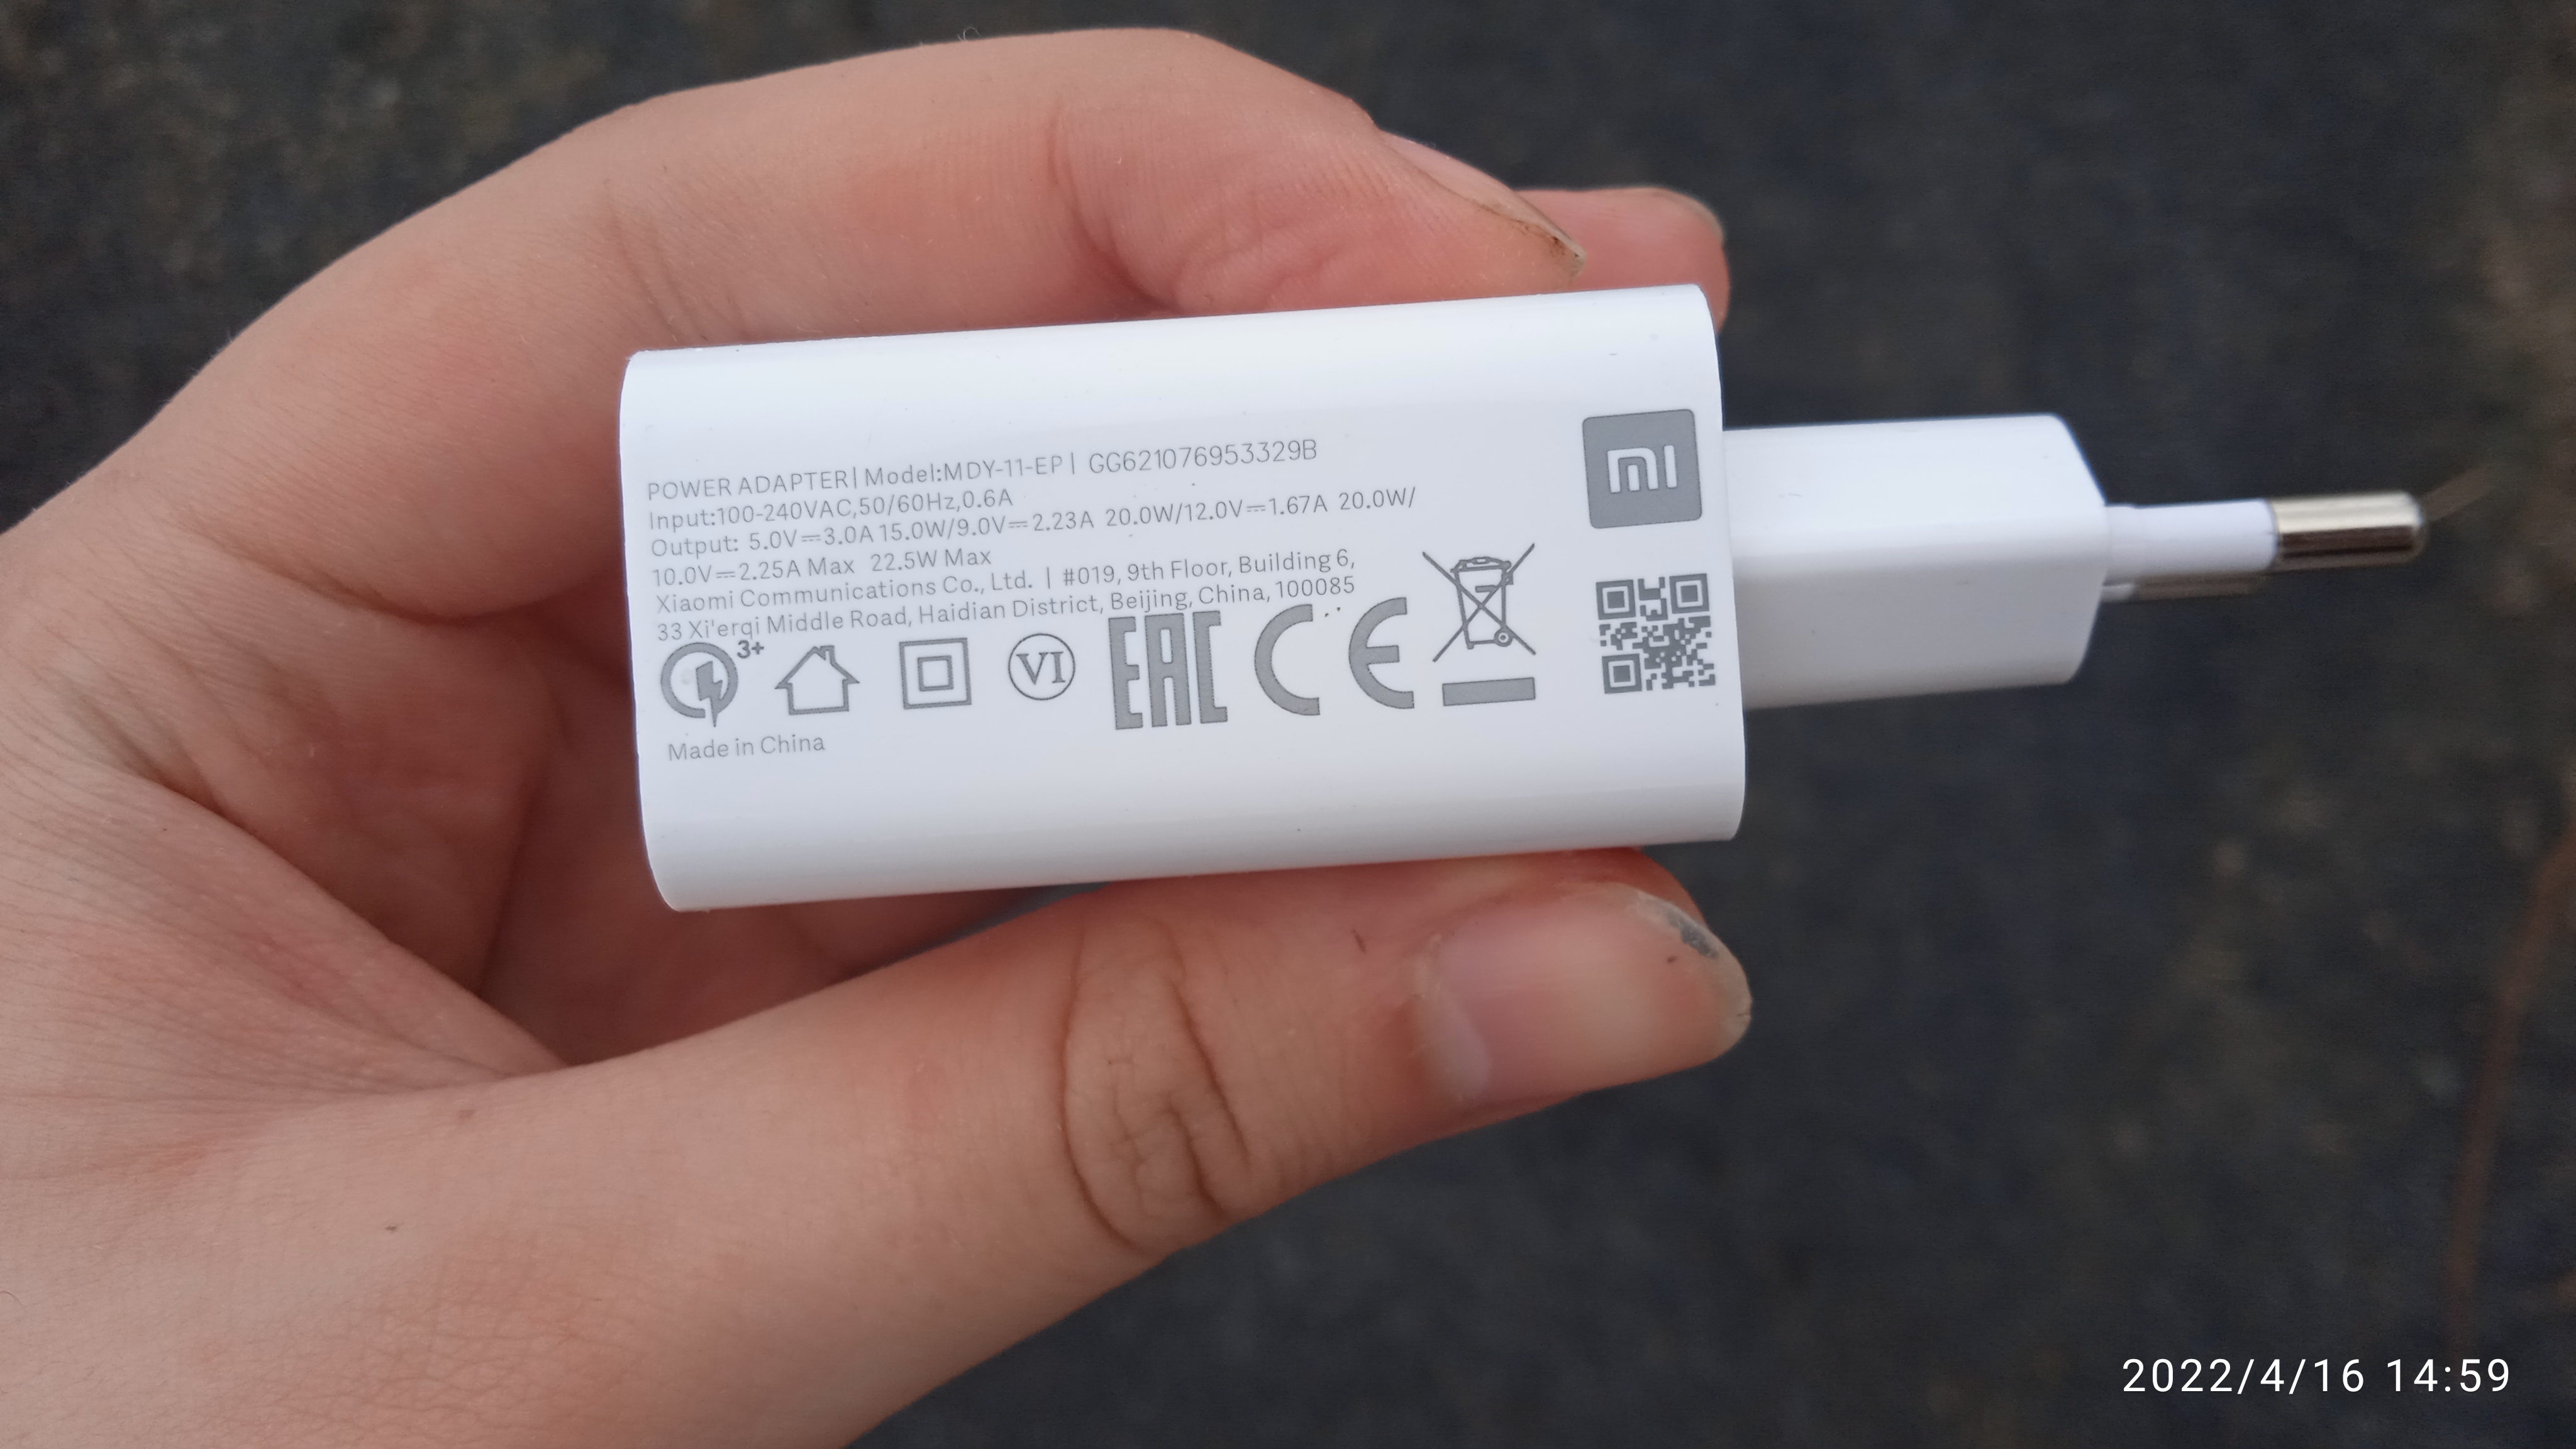
\includegraphics[scale=0.035]{fig/lec01/charger_3.jpg}
			\caption{Generic mobile phone charger (source: \href{https://commons.wikimedia.org/wiki/File:Charger_Xioami.jpg}{Wikimedia Commons}, Radio Mayak Pervouralsk, \href{https://creativecommons.org/licenses/by-sa/4.0/}{CC BY-SA 4.0})}
		\end{subfigure}
		\begin{subfigure}[t]{0.4\textwidth}
			\centering
			\includegraphics[scale=0.15]{fig/lec01/EV.jpg}
			\caption{Example electric vehicle (source: \href{https://commons.wikimedia.org/wiki/File:IBMTorontoSoftwareLabEVChargers4.jpg}{Wikimedia Commons}, Raysonho \href{https://creativecommons.org/publicdomain/zero/1.0/deed.en}{CCo 1.0})}
		\end{subfigure}
	\end{figure}
\end{frame}

%%%%%%%%%%%%%%%%%%%%%%%%%%%%%%%%%%%%%%%%%%%%%%%%%%%%%%%%%%%%%
%% Where do you find active and passive components %%
%%%%%%%%%%%%%%%%%%%%%%%%%%%%%%%%%%%%%%%%%%%%%%%%%%%%%%%%%%%%%
\begin{frame}
	\frametitle{Locating active and passive components in real world}
	\begin{figure}
		\centering
		%\hfill
		\begin{subfigure}[t]{0.4\textwidth}
			\centering
			\includegraphics[scale=0.035]{fig/lec01/wind_turbine.jpg}
			\caption{Thorntonbank Wind Farm, using 5 MW turbines REpower 5M in the North Sea off the coast of Belgium (source: \href{https://en.wikipedia.org/wiki/File:Windmills_D1-D4_(Thornton_Bank).jpg}{Wikimedia Commons}, © Hans Hillewaert, \href{https://creativecommons.org/licenses/by-sa/4.0/}{CC BY-SA 4.0})}
		\end{subfigure}
		\begin{subfigure}[t]{0.4\textwidth}
			\centering
			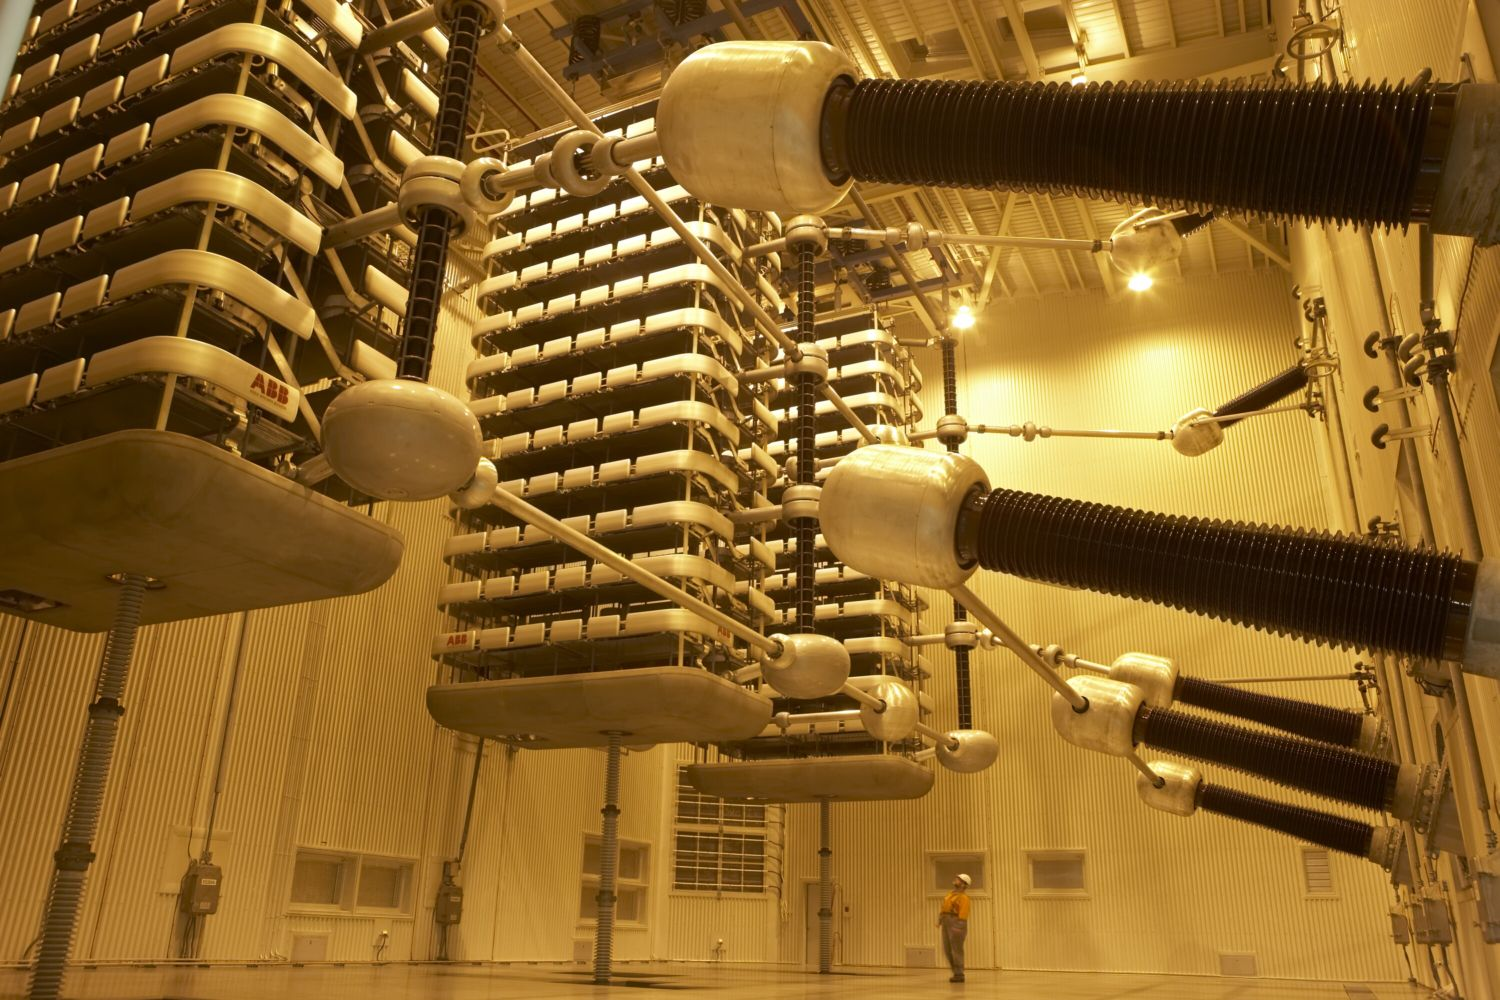
\includegraphics[scale=0.5]{fig/lec01/Thyristor.jpg}
			\caption{Thyristor valve in an HVDC (source: \href{https://commons.wikimedia.org/wiki/File:Pole_2_Thyristor_Valve.jpg}{Wikimedia Commons}, Marshelec, \href{https://creativecommons.org/licenses/by-sa/3.0}{CC BY-SA 3.0})}
		\end{subfigure}
	\end{figure}
\end{frame}

%%%%%%%%%%%%%%%%%%%%%%%%%%%%%%%%%%%%%%%%%%%%%%%%%%%%%%%%%%%%%
%% Where do you find active and passive components %%
%%%%%%%%%%%%%%%%%%%%%%%%%%%%%%%%%%%%%%%%%%%%%%%%%%%%%%%%%%%%%
\begin{frame}
	\frametitle{Locating active and passive components in real world}
	\begin{figure}
		\centering
		%\hfill
		\begin{subfigure}[t]{0.4\textwidth}
			\centering
			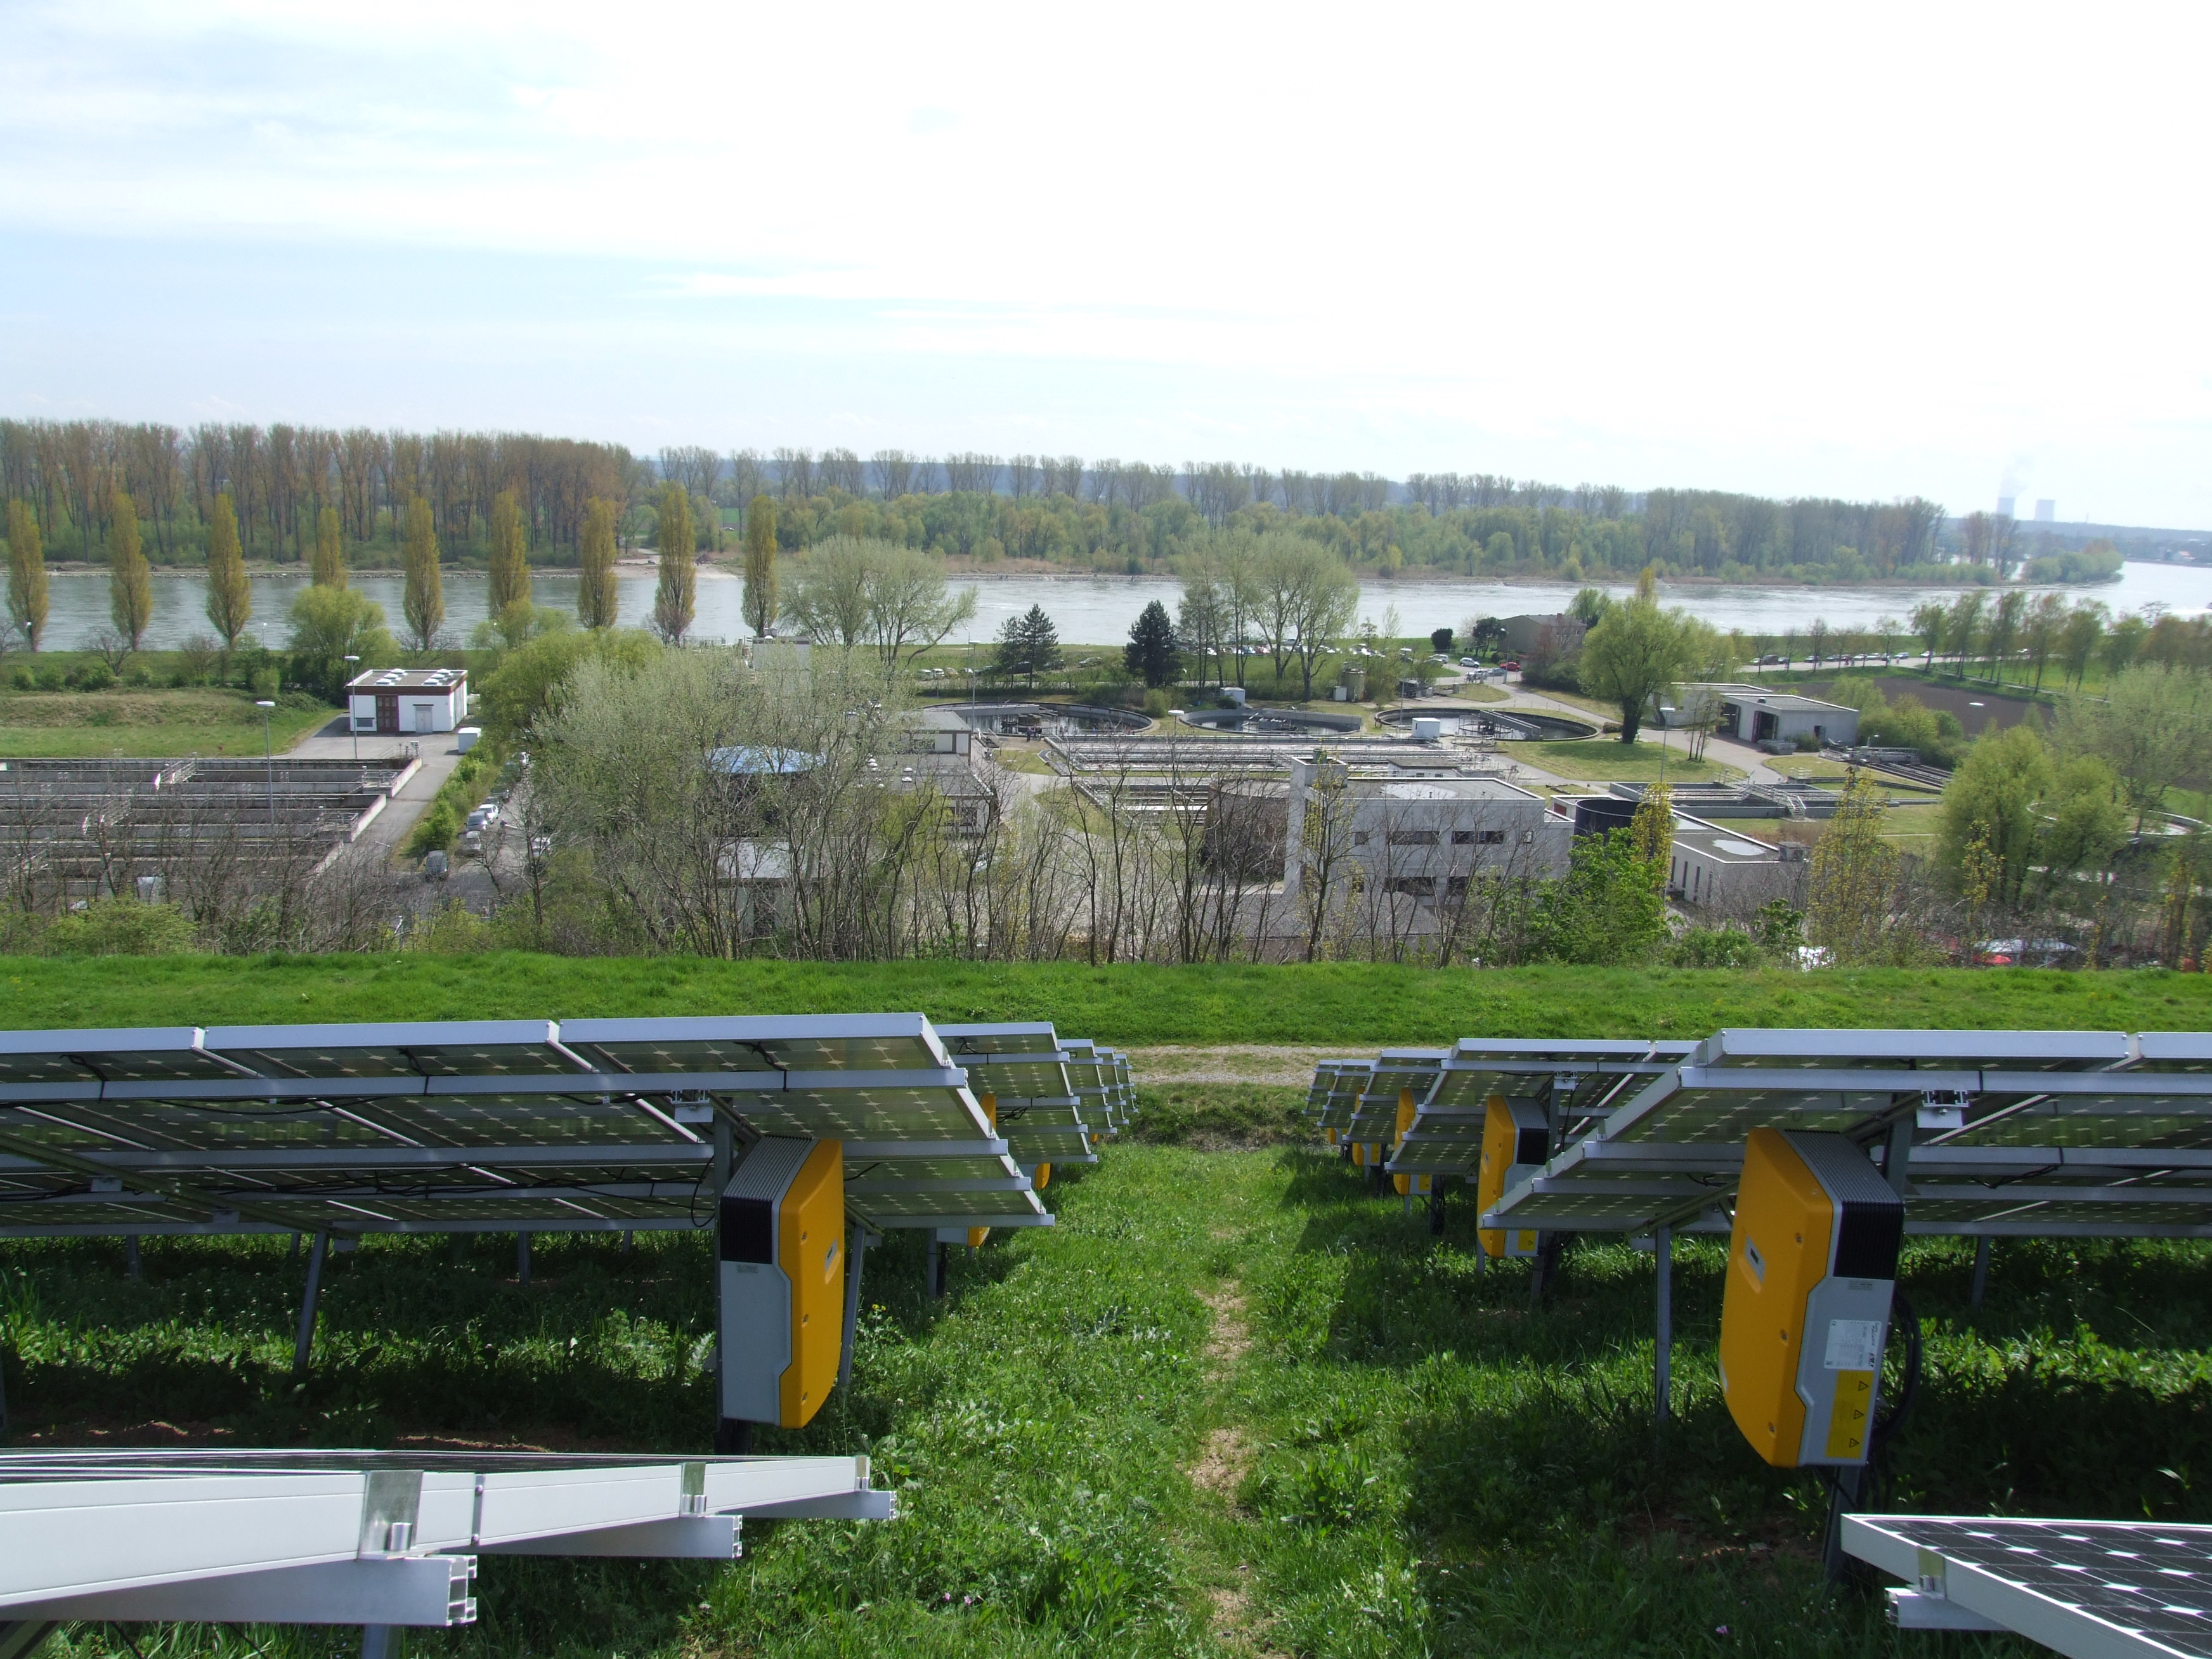
\includegraphics[scale=0.05]{fig/lec01/solar_inverter.jpg}
			\caption{A solar PV plant in  (source: \href{https://commons.wikimedia.org/wiki/File:Müllberg_Speyer_-_6_-_Rückseite_der_östlichen_Solarpanele.JPG}{Wikimedia Commons}, Claus Ableiter,\href{https://creativecommons.org/licenses/by-sa/3.0}{CC BY-SA 3.0})}
		\end{subfigure}
		\begin{subfigure}[t]{0.4\textwidth}
			\centering
			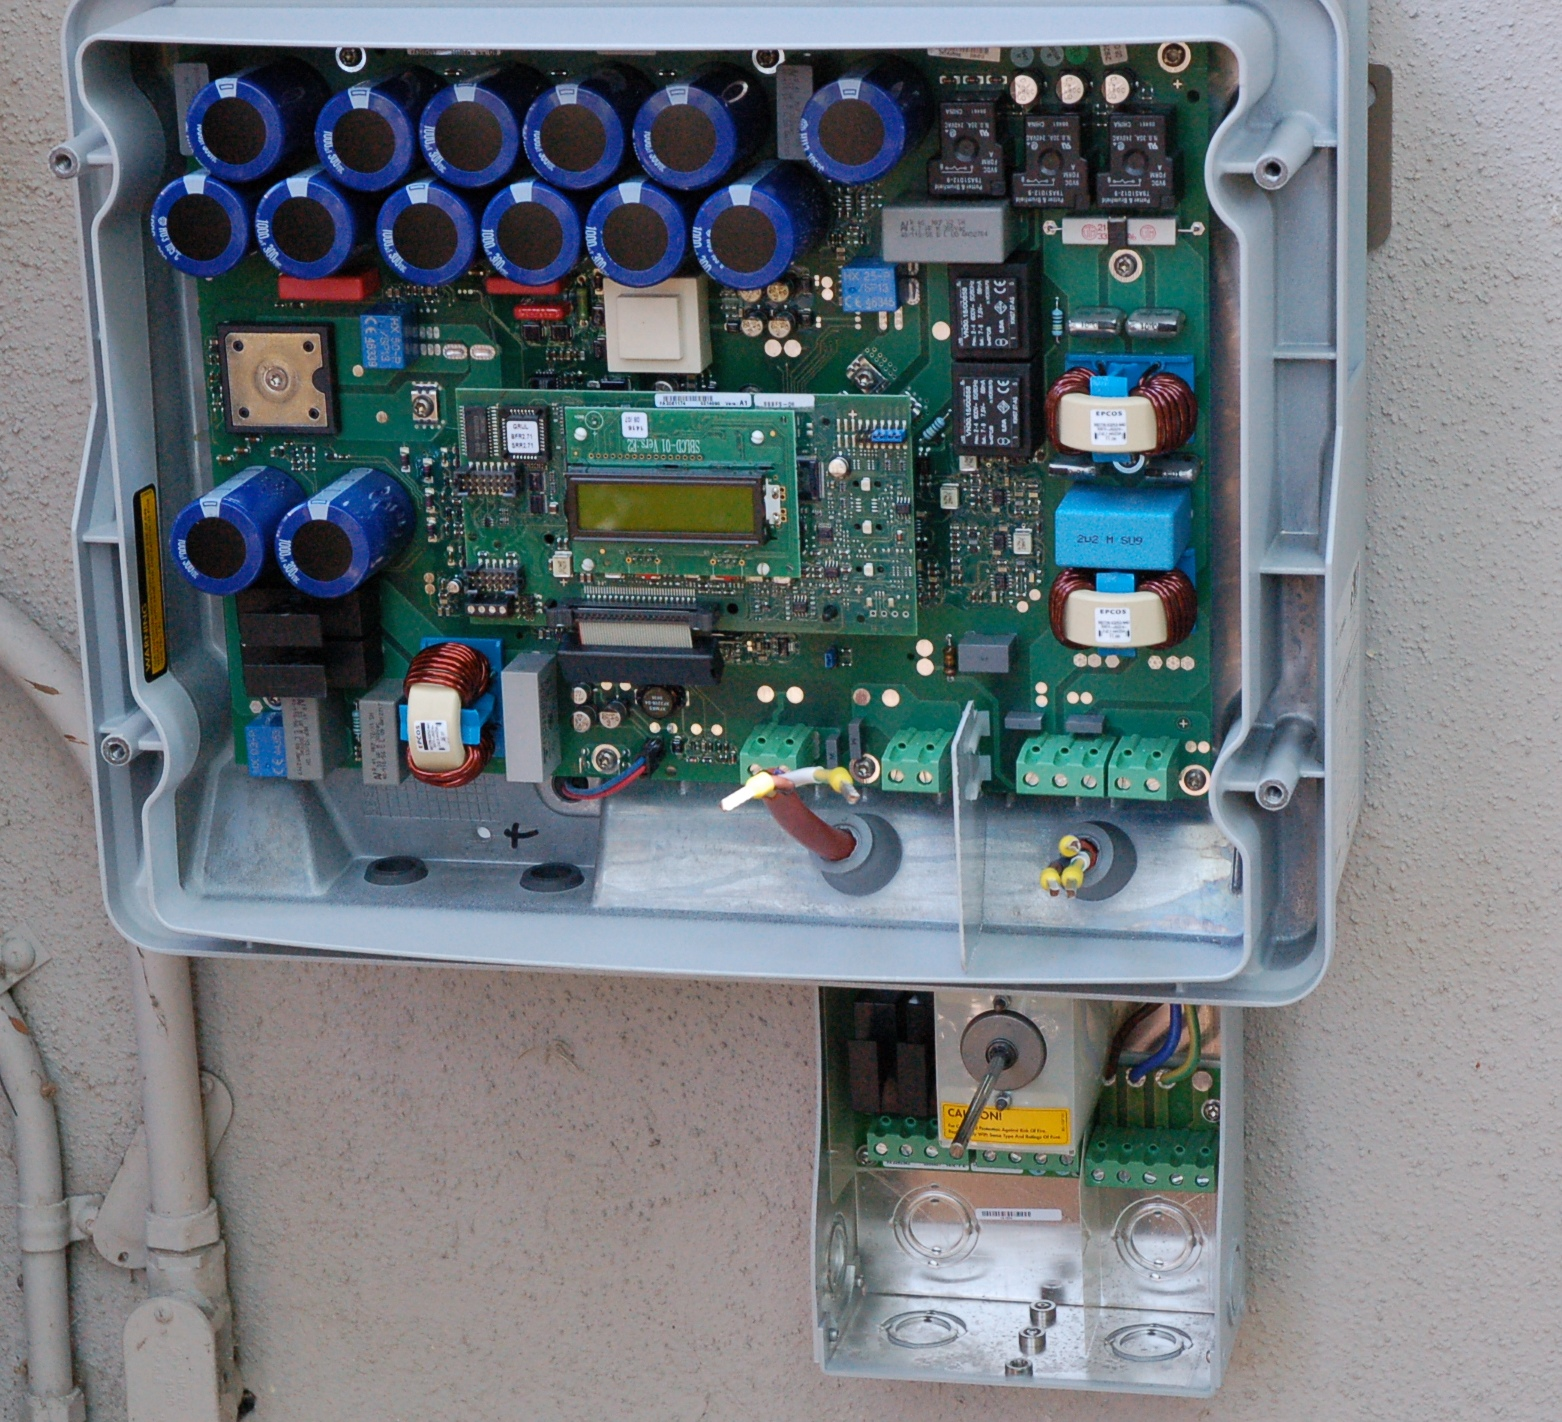
\includegraphics[scale=0.1]{fig/lec01/solar_inverter_open.jpg}
			\caption{Internal view of a solar inverter (source: \href{https://commons.wikimedia.org/wiki/File:Sunny_Boy_3000.jpg}{Wikimedia Commons}, Russell Neches, \href{https://creativecommons.org/licenses/by/2.0/}{CC BY 2.0})}
		\end{subfigure}
	\end{figure}
\end{frame}

%%%%%%%%%%%%%%%%%%%%%%%%%%%%%%%%%%%%%%%%%%%%%%%%%%%%%%%%%%%%%
%% Why are electric machines and drives important ? %%
%%%%%%%%%%%%%%%%%%%%%%%%%%%%%%%%%%%%%%%%%%%%%%%%%%%%%%%%%%%%%
\begin{frame}
	\frametitle{Why is knowledge about power electroics devices is important?}
	\begin{varblock}{Power Electronics more relevant than ever}
		Knowledge of power electronics devices is crucial for designing efficient systems that convert, control, and deliver electrical energy. It enables innovation in EVs, renewable energy, robotics, and industrial automation by optimizing performance, minimizing losses, and ensuring reliable operation. 
	\end{varblock}
	\begin{varblock}{Power electronics is the key to efficiency and sustainability}<2->
		Power electronic systems handle and convert more than 70\% of global electricity across industries such as transportation, energy, and automation (source: \href{https://www.hitachienergy.com/news-and-events/perspectives/2021/08/power-electronics-revolutionizing-the-world-s-future-energy-systems}{International Energy Agency}). With rising demands for electrification, advancing device efficiency and reliability is critical to minimizing energy losses, improving system performance, and enabling sustainable technologies across the globe.
	\end{varblock}
\end{frame}

%%%%%%%%%%%%%%%%%%%%%%%%%%%%%%%%%%%%%%%%%%%%%%%%%%%%%%%%%%%%%
%% Breakdown of an inductor %%
%%%%%%%%%%%%%%%%%%%%%%%%%%%%%%%%%%%%%%%%%%%%%%%%%%%%%%%%%%%%%
\begin{frame}
	\frametitle{Looking inside to define objectives!}
	%\vspace{-1cm}
	\begin{figure}
		\centering
		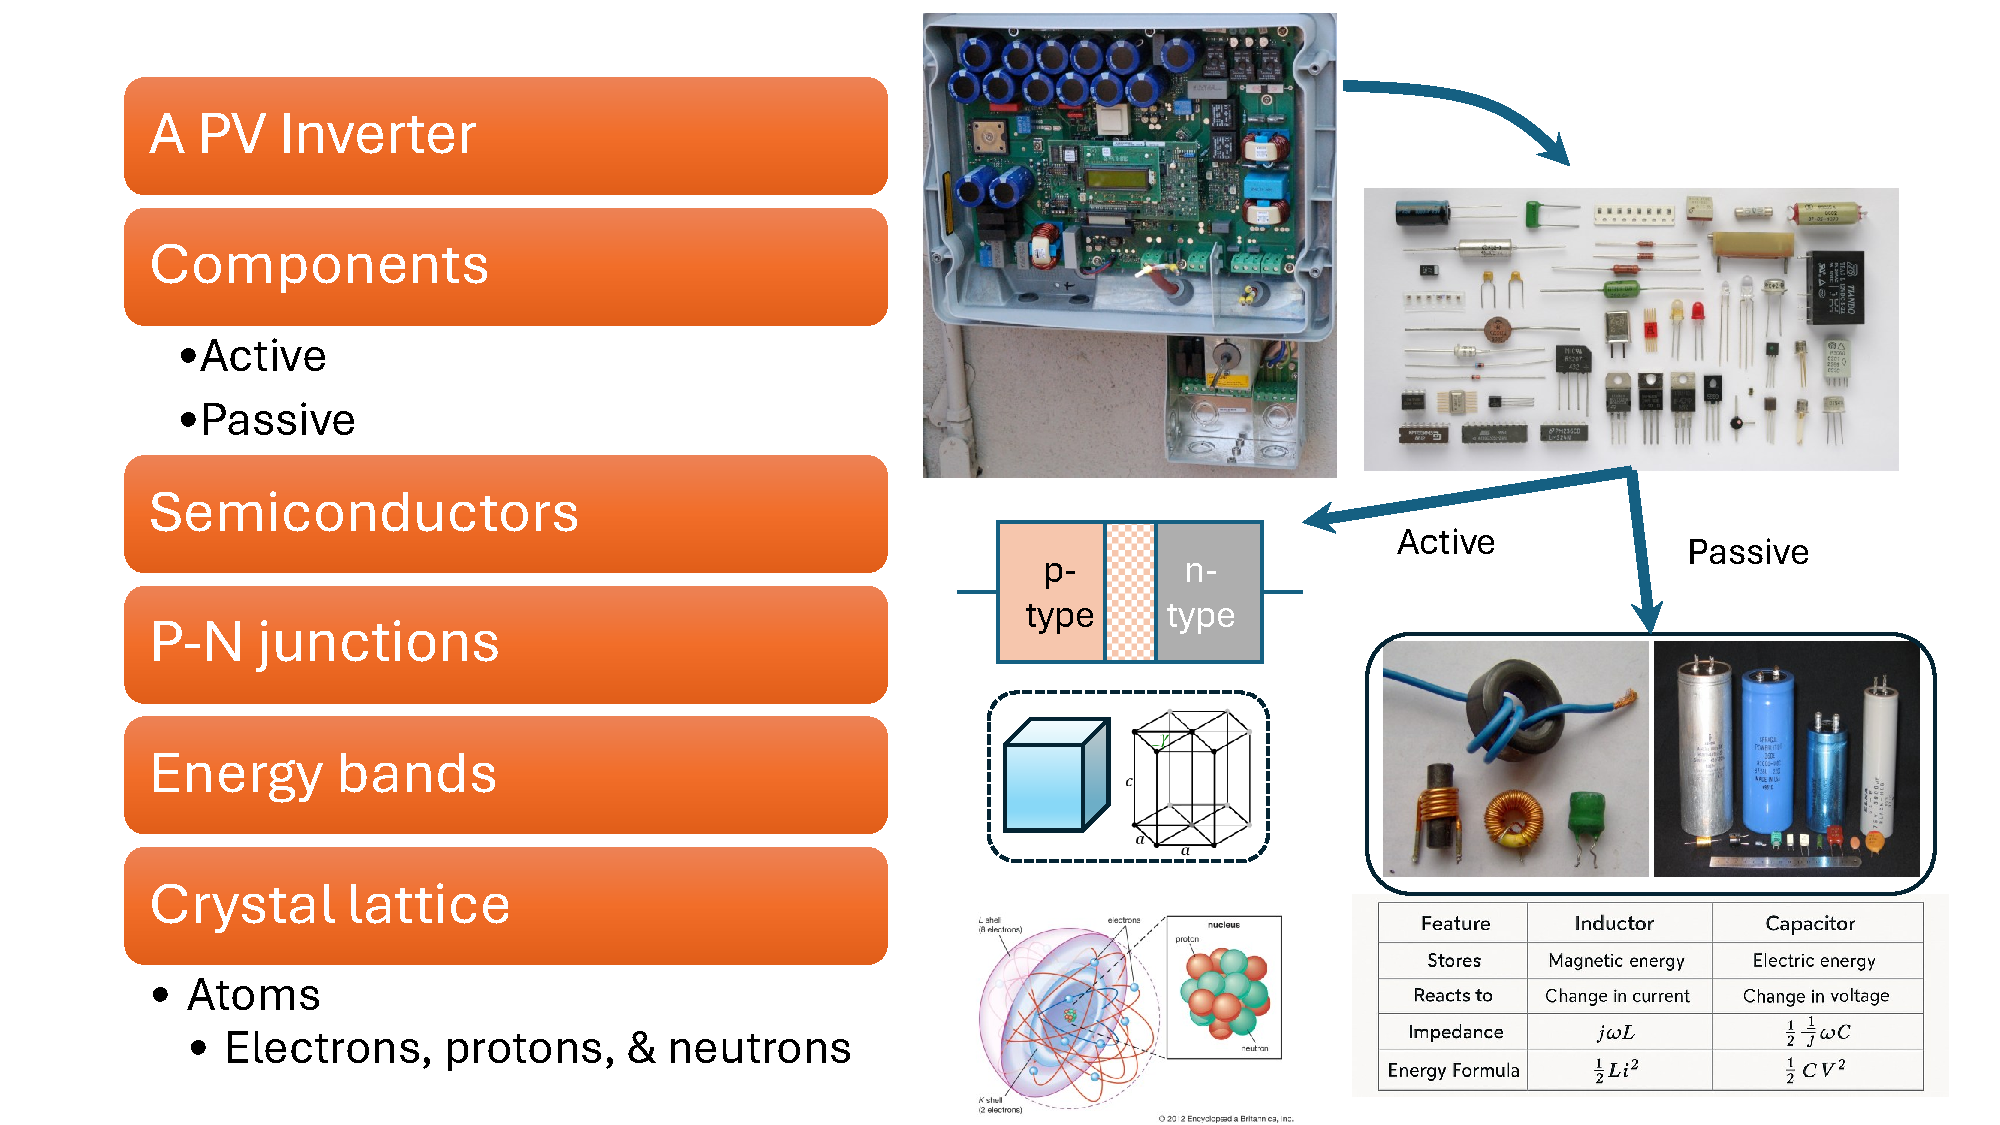
\includegraphics[scale=0.35]{fig/lec01/Flow_of_components.pdf}
		\caption{Definition of course and need (source: PV inverter, components, inductors, and capacitors \href{https://commons.wikimedia.org/wiki/Main_Page}{Wikimedia Commons}, multiple sources, public domain)}
	\end{figure}
\end{frame}

%%%%%%%%%%%%%%%%%%%%%%%%%%%%%%%%%%%%%%%%%%%%%%%%%%%%%%%%%%%%%
%% Learning objectives %%
%%%%%%%%%%%%%%%%%%%%%%%%%%%%%%%%%%%%%%%%%%%%%%%%%%%%%%%%%%%%%
\begin{frame}
	\frametitle{Learning objectives}
	\begin{itemize}
		\item Understand and explain the role of power electronics in modern energy systems, electrification, and sustainable technologies. 
		\item Understand the working principles of each device and components in power electronics.
		\item Analyze the physics of semiconductor materials and devices, including band theory, carrier transport, junction behavior, and breakdown mechanisms.
		\item Differentiate and evaluate the characteristics, structures, and operation principles of power semiconductor devices.
		\item Interpret and model switching characteristics, conduction behavior, and thermal limitations of conventional and wide-bandgap power devices (Si, SiC, GaN).
		\item Select and model active and passive components such as capacitors, inductors, transformers, and filters with consideration of frequency, losses, and application context.
		\item Have fun learning about power electronics devices and components.
	\end{itemize}
\end{frame}

%%%%%%%%%%%%%%%%%%%%%%%%%%%%%%%%%%%%%%%%%%%%%%%%%%%%%%%%%%%%%
%% Necessary prior knowledge %%
%%%%%%%%%%%%%%%%%%%%%%%%%%%%%%%%%%%%%%%%%%%%%%%%%%%%%%%%%%%%%
\begin{frame}
	\frametitle{Necessary prior knowledge for this course}
	You should have a basic understanding of the following topics:
	\begin{itemize}
		\item Basic electrical engineering knowledge (e.g., Ohm's law, Kirchhoff's laws, etc.)
		\item Basic understanding of physics in electronics
		\item Algebra and complex numbers
		\item Basic signal theory knowledge (e.g., Fourier series, Laplace transform)
		\item No advanced knowledge of semiconductors or programming is needed — this course builds those concepts from scratch and applies them to real systems.
	\end{itemize}
	\vspace{0.5cm}
	\onslide<2->What we will \underline{not} cover, but you do not need to know (covered in separate courses):
	\begin{itemize}
		\item Power converter circuits and topologies.
		\item Power electronics in depth involving analysis and controller design. 
	\end{itemize}
\end{frame}

%%%%%%%%%%%%%%%%%%%%%%%%%%%%%%%%%%%%%%%%%%%%%%%%%%%%%%%%%%%%%
%% Recommended reading %%
%%%%%%%%%%%%%%%%%%%%%%%%%%%%%%%%%%%%%%%%%%%%%%%%%%%%%%%%%%%%%
\begin{frame}
	\frametitle{Recommended reading}
	\begin{itemize}
		\item Baliga, B. Jayant. Fundamentals of power semiconductor devices. Springer Science \& Business Media, 2010.
		\item Lutz, Josef, Heinrich Schlangenotto, Uwe Scheuermann, and Rik De Doncker. "Semiconductor power devices." Physics, characteristics, reliability 2 (2011).
		\item Baliga, B. Jayant, ed. Wide Bandgap Semiconductor Power Devices: Materials, Physics, Design, and Applications. Woodhead Publishing, 2018.
		\item K. Niayesh, M. Runde, "Power Switching Components Theory, Applications and Future Trends", 1. Ed., Springer, 2018.
	\end{itemize}
\end{frame} % Overview / introduction
\section{Physics of Basic Semiconductor Devices}
\title[Physics]{Physics of basic semiconductor devices}  

\begin{frame}[plain]
    \titlepage
\end{frame}

%%%%%%%%%%%%%%%%%%%%%%%%%%%%%%%%%%%%%%%%%%%%%%%%%%%%%%%%%%%%%
%% Introduction to the module %%
%%%%%%%%%%%%%%%%%%%%%%%%%%%%%%%%%%%%%%%%%%%%%%%%%%%%%%%%%%%%%
\begin{frame}
    \frametitle{What will you learn?}
\begin{itemize}
    \item Materials
        \begin{itemize}
            \item Atoms and materials used in semiconductors
            \item Flow of electrons and holes
            \item Conductors, insulators, and semiconductors
            \item Energy bands, Fermi level, doping
            \item Intrinsic and extrinsic semiconductors
        \end{itemize}
    \item Fundamental properties
        \begin{itemize}
            \item Carrier concentration 
            \item Carrier mobility
            \item The Hall effect
            \item Drift and diffusion currents
            \item Breakdown voltage, temerature dependence, etc.
        \end{itemize}
    \item pn junctions
        \begin{itemize}
            \item What is a pn junction?
            \item Diodes and their characteristics
            \item Physics of operaiton, properties and IV characteristics of diodes.
        \end{itemize}
\end{itemize}
\end{frame}

%%%%%%%%%%%%%%%%%%%%%%%%%%%%%%%%%%%%%%%%%%%%%%%%%%%%%%%%%%%%%
%% Atoms %%
%%%%%%%%%%%%%%%%%%%%%%%%%%%%%%%%%%%%%%%%%%%%%%%%%%%%%%%%%%%%%
\begin{frame}
	\frametitle{Atoms}
	\begin{columns}
		\begin{column}{0.65\textwidth}
          \begin{itemize}
            \item All matter is made up of atoms.
            \item Atoms are the smallest unit of matter that retains the properties of an element.
            \item Two models of atom exist: classical and quantum.
            \item The classical model of the atom is based on the idea that atoms are made up of a nucleus (protons and neutrons) surrounded by electrons that orbit the nucleus in fixed paths- Rutherford's Atomic Model
            \item The quantum model of the atom is based on the principles of quantum mechanics, which describe the behaviour of particles at the atomic and subatomic quantised energy levels- Bohr's Atomic Model:
            \item Both model states: atoms consist of a nucleus (protons \& neutrons) \& electrons that orbit the nucleus.
          \end{itemize}
		\end{column}
        \hfill
		\begin{column}{0.35\textwidth}
            \begin{figure}
                \centering
                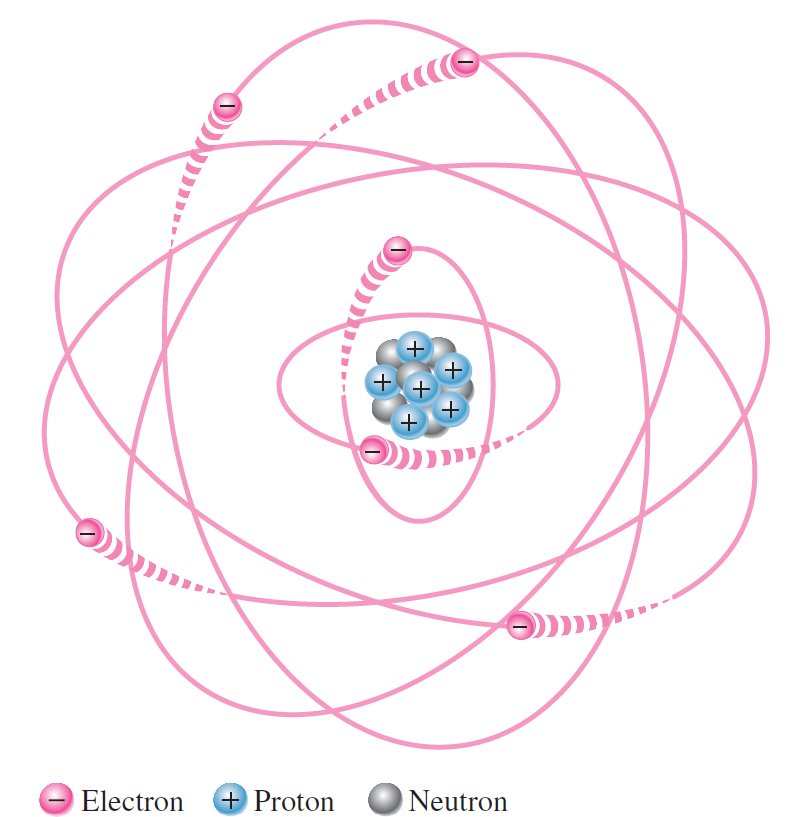
\includegraphics[width=0.8\textwidth]{fig/lec02/Atom_model.png}
                \caption{The Bohr model of an atom (Adapted from \href{https://www.pearson.com/en-us/subject-catalog/p/electronic-devices-electron-flow-version/P200000001048/9780137556755}{Electronic Devices (Electron Flow Version), 10th edition})}
            \end{figure}
		\end{column}
		\end{columns}
\end{frame}


%%%%%%%%%%%%%%%%%%%%%%%%%%%%%%%%%%%%%%%%%%%%%%%%%%%%%%%%%%%%%
%% Atoms continued %%
%%%%%%%%%%%%%%%%%%%%%%%%%%%%%%%%%%%%%%%%%%%%%%%%%%%%%%%%%%%%%
\begin{frame}
	\frametitle{Atoms}
	\begin{columns}
		\begin{column}{0.65\textwidth}
          \begin{itemize}
            \item The number of protons in the nucleus determines the element (e.g., hydrogen, oxygen, etc.).
            \item Electrons are arranged in energy levels or shells around the nucleus.
            \item Electrons are negatively charged, while protons are positively charged.
            \item Number of protons in the nucleus is equal to the number of electrons in the atom, making it electrically neutral.
            \item Outermost shell of an atom is called the valence shell.
            \item Number of electrons in the valence shell, also called valence electrons determines the chemical properties of the atom.
            \item Atoms can gain or lose electrons to form ions, which are charged particles.
          \end{itemize}
		\end{column}
        \hfill
		\begin{column}{0.35\textwidth}
            \begin{figure}
                \centering
                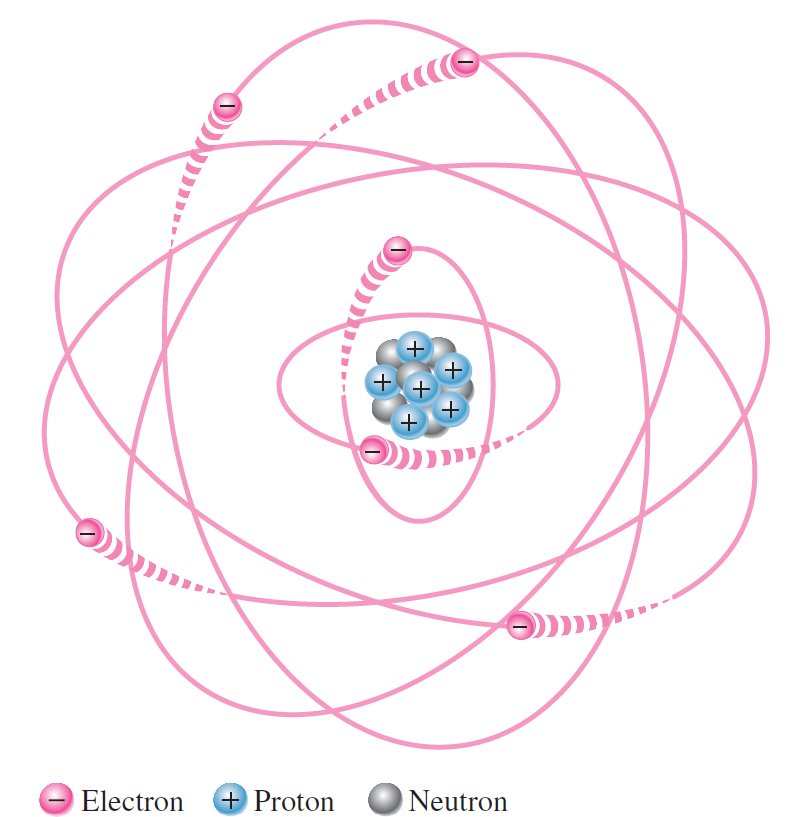
\includegraphics[width=0.8\textwidth]{fig/lec02/Atom_model.png}
                \caption{The Bohr model of an atom (Adapted from \href{https://www.pearson.com/en-us/subject-catalog/p/electronic-devices-electron-flow-version/P200000001048/9780137556755}{Electronic Devices (Electron Flow Version), 10th edition})}
            \end{figure}
		\end{column}
		\end{columns}
\end{frame}

%%%%%%%%%%%%%%%%%%%%%%%%%%%%%%%%%%%%%%%%%%%%%%%%%%%%%%%%%%%%%
%% Ionisation energy %%
%%%%%%%%%%%%%%%%%%%%%%%%%%%%%%%%%%%%%%%%%%%%%%%%%%%%%%%%%%%%%
\begin{frame}
	\frametitle{Ionisation energy}
          \begin{itemize}
            \item The energy required to remove an electron from an atom is called ionisation energy.
            \item The ionisation energy varies for different elements and is generally higher for elements with more protons in the nucleus.
            \item The ionisation energy is also affected by the distance of the electron from the nucleus and the number of electrons in the valence shell- outermost shell is more vulnerable to ionisation!
            \item Atoms with low ionisation energy tend to lose electrons easily and form positive ions, while atoms with high ionisation energy tend to gain electrons and form negative ions.
            \item The ionisation energy is an important factor in determining the chemical reactivity of an element.
          \end{itemize}
\end{frame}


%%%%%%%%%%%%%%%%%%%%%%%%%%%%%%%%%%%%%%%%%%%%%%%%%%%%%%%%%%%%%
%% Materials %%
%%%%%%%%%%%%%%%%%%%%%%%%%%%%%%%%%%%%%%%%%%%%%%%%%%%%%%%%%%%%%
\begin{frame}
	\frametitle{Materials in electronics}
	\begin{columns}
		\begin{column}{0.6\textwidth}
            \begin{itemize}
                \item The electrical properties of materials are determined by the arrangement and behaviour of their atoms and electrons.
                \item Example: Carbon (C) has 4 valence electrons.
                \item Nucleus of C: has 6 protons and 6 neutrons. 2 electrons in the inner shell/core make a charge of +4 in the core.
                \item 4 valence electrons in the outer shell, forms covalent bonds with other atoms. 
                \item In solids like diamond or any organic compounds, each carbon atom is tightly bonded to 4 others in a 3D lattice — \textbf{no free electrons to move around}.
                \item So, carbon is a non-metal and is a poor conductor of electricity. 
            \end{itemize}
		\end{column}
        \hfill
		\begin{column}{0.4\textwidth}
            \begin{figure}
                \centering
                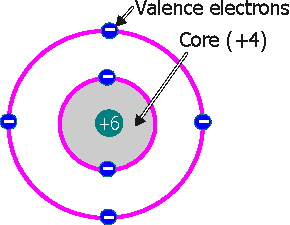
\includegraphics[width=0.8\textwidth]{fig/lec02/carbon_atom.pdf}
                \caption{Carbon atom with four valence electrons- used in resistors but if you \textbf{change crystal structure} (example graphite, where one electron is free to move due to flat layers of carbon atoms)}
            \end{figure}
		\end{column}
		\end{columns}
\end{frame}

%%%%%%%%%%%%%%%%%%%%%%%%%%%%%%%%%%%%%%%%%%%%%%%%%%%%%%%%%%%%%
%% Insulators, conductors and semiconductors %%
%%%%%%%%%%%%%%%%%%%%%%%%%%%%%%%%%%%%%%%%%%%%%%%%%%%%%%%%%%%%%
\begin{frame}
	\frametitle{Materials in electronics}
            \begin{itemize}
                \item The electrical properties of materials can be classified into three categories based on their ability to conduct electricity:
            \begin{itemize}
                \item \textbf{Insulators} have valence electrons tightly bound to the atoms and do not have free electrons to conduct electricity. Insulators have a \textbf{very high ionisation energy}, meaning they require a lot of energy to remove an electron from the atom. So they are bad conductors of electricity. Examples: rubber, glass, and plastic.
                \item \textbf{Conductors} have a large number of loosly bounded electrons that can move easily through the material, allowing them to conduct electricity well. Conductors have a \textbf{low ionisation energy}, meaning they require very little energy to remove an electron from the atom. So, they have a low resistance to the flow of electric current. Examples: metals like copper (Cu) and aluminum (Al).
                \item \textbf{Semiconductors*} in pure or intrinsic state is neither a good conductor nor a good insulator. They have to be synthesized as compounds or made extrinsic by adding impurities (doping) to change their electrical properties. Examples: Silicon (Si) and Germanium (Ge) as intrinsic and gallium arsenide, indium phosphide, gallium nitride, silicon carbide are extrinsic.
            \end{itemize}
            \end{itemize}
            *Semiconductors can conduct electricity under certain conditions, such as when they are doped with impurities or when they are exposed to light or heat.
\end{frame}

%%%%%%%%%%%%%%%%%%%%%%%%%%%%%%%%%%%%%%%%%%%%%%%%%%%%%%%%%%%%%
%% Ask about explanation based on Bohr model of atom %%
%%%%%%%%%%%%%%%%%%%%%%%%%%%%%%%%%%%%%%%%%%%%%%%%%%%%%%%%%%%%%
\begin{frame}
	\frametitle{Example explanation based on Bohr model of atom}
        \begin{figure}
            \centering
            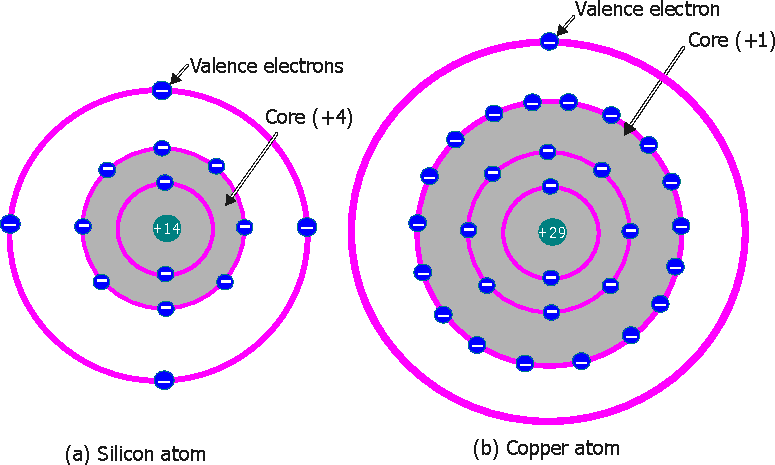
\includegraphics[width=0.7\textwidth]{fig/lec02/Cu_Si_atom1.pdf}
            \caption{(a) Silicon atom with four valence electrons, (b) Copper atom with one valence electron}
        \end{figure}
\end{frame}

%%%%%%%%%%%%%%%%%%%%%%%%%%%%%%%%%%%%%%%%%%%%%%%%%%%%%%%%%%%%%
%% Explanation based on Bohr model of atom %%
%%%%%%%%%%%%%%%%%%%%%%%%%%%%%%%%%%%%%%%%%%%%%%%%%%%%%%%%%%%%%
\begin{frame}
	\frametitle{Example explanation based on Bohr model of atom}
	\begin{columns}
		\begin{column}{0.6\textwidth}
            \begin{itemize}
                \item \textbf{Semiconductor}: Silicon
                \item Silicon (Si) has 4 valence electrons.
                \item Nucleus of Si: has 14 protons and 14 neutrons. 10 electrons in the inner shell/core make a charge of +4 in the core.
                \item 4 valence electrons in the outer shell, forms covalent bonds with other atoms.
                \item In solids like those forming an organic compounds, each silicon atom is tightly bonded to 4 others in a 3D lattice — \textbf{no free electrons to move around}.
                \item So, silicon is a non-metal and is a poor conductor of electricity.
            \end{itemize}
		\end{column}
        \hfill
		\begin{column}{0.4\textwidth}
            \begin{figure}
                \centering
                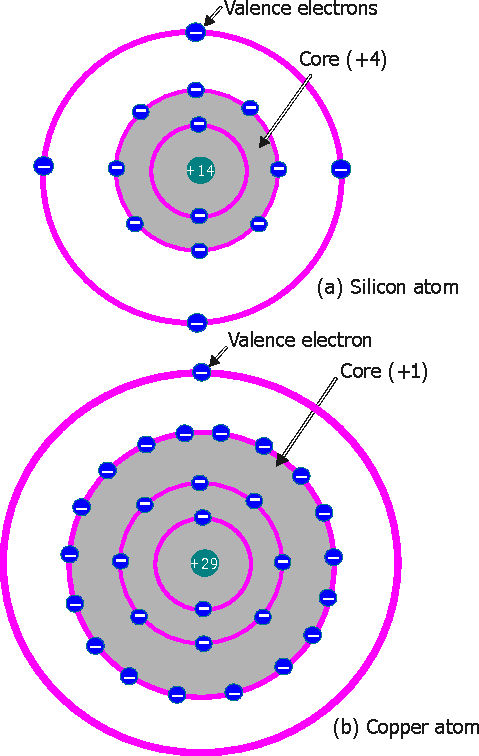
\includegraphics[width=0.6\textwidth]{fig/lec02/Cu_Si_atom.pdf}
                \caption{(a) Silicon atom with four valence electrons, (b) Copper atom with one valence electron}
            \end{figure}
		\end{column}
		\end{columns}
\end{frame}

%%%%%%%%%%%%%%%%%%%%%%%%%%%%%%%%%%%%%%%%%%%%%%%%%%%%%%%%%%%%%
%% Explanation based on Bohr model of atom %%
%%%%%%%%%%%%%%%%%%%%%%%%%%%%%%%%%%%%%%%%%%%%%%%%%%%%%%%%%%%%%
\begin{frame}
	\frametitle{Example explanation based on Bohr model of atom}
	\begin{columns}
		\begin{column}{0.6\textwidth}
            \begin{itemize}
                \item \textbf{Conductor}: Copper
                \item Copper (Cu) has 1 valence electron.  
                \item Nucleus of Cu: has 29 protons and 29 neutrons. 28 electrons in the inner shell/core make a charge of +1 in the core.
                \item 1 valence electron in the outer shell, forms metallic bonds with other atoms.
                \item In solids like copper, each copper atom is loosely bonded to other atoms in a 3D lattice — \textbf{free electrons to move around}.
                \item So, copper is a metal and is a good conductor of electricity.
            \end{itemize}
		\end{column}
        \hfill
		\begin{column}{0.4\textwidth}
            \begin{figure}
                \centering
                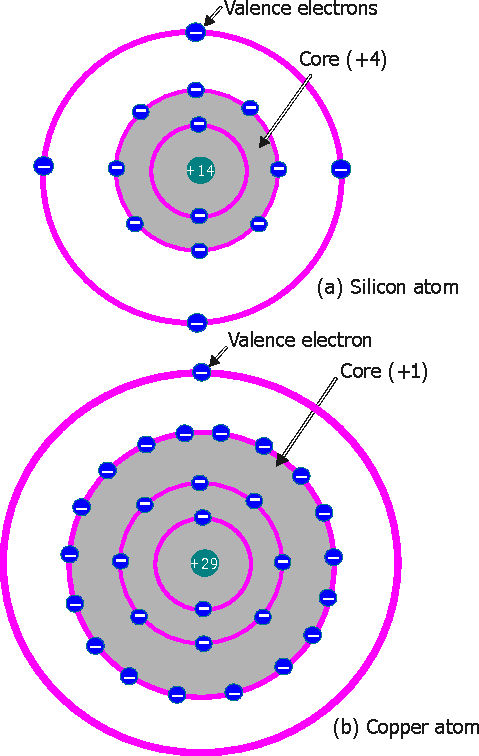
\includegraphics[width=0.6\textwidth]{fig/lec02/Cu_Si_atom.pdf}
                \caption{(a) Silicon atom with four valence electrons, (b) Copper atom with one valence electron}
            \end{figure}
		\end{column}
		\end{columns}
\end{frame}

%%%%%%%%%%%%%%%%%%%%%%%%%%%%%%%%%%%%%%%%%%%%%%%%%%%%%%%%%%%%%
%% Total energy of the electron %%
%%%%%%%%%%%%%%%%%%%%%%%%%%%%%%%%%%%%%%%%%%%%%%%%%%%%%%%%%%%%%
\begin{frame}
	\frametitle{Energy of electron in an orbit}
    \begin{columns}
        \begin{column}{0.6\textwidth}
            \begin{itemize}
                \item The energy of an electron in an orbit is determined by the distance of the electron from the nucleus and the number of protons in the nucleus.
                \item Electrons in orbits closer to the nucleus have lower energy than those in orbits farther away.
                \item The energy of an electron in an orbit is also affected by the presence of other electrons in the atom.
                \item Electrons in the same shell repel each other, which can increase their energy and make them more likely to be ionised.
                \item \textbf{Why is electron having a negative charge?}
            \end{itemize}
        \end{column}
        \hfill
        \begin{column}{0.4\textwidth}
            \begin{figure}
                \centering
                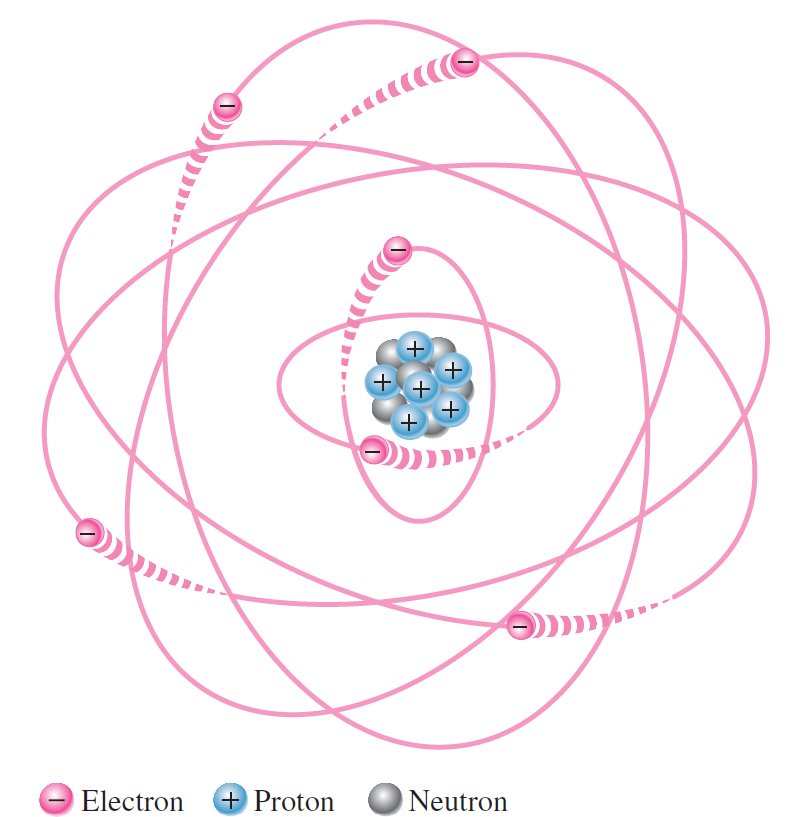
\includegraphics[width=0.8\textwidth]{fig/lec02/Atom_model.png}
                \caption{The Bohr model of an atom (Adapted from \href{https://www.pearson.com/en-us/subject-catalog/p/electronic-devices-electron-flow-version/P200000001048/9780137556755}{Electronic Devices (Electron Flow Version), 10th edition})}
            \end{figure}
        \end{column}
        \end{columns}
\end{frame}

%%%%%%%%%%%%%%%%%%%%%%%%%%%%%%%%%%%%%%%%%%%%%%%%%%%%%%%%%%%%%
%% Total energy of the electron %%
%%%%%%%%%%%%%%%%%%%%%%%%%%%%%%%%%%%%%%%%%%%%%%%%%%%%%%%%%%%%%
\begin{frame}
	\frametitle{Total energy of the electron}
    \begin{itemize}
        \item The planetary model of atom developed by \textbf{Niels Bohr} in 1913, where electrons are thought to orbit the nucleus like planets orbiting the sun. \textit{The nucleus is considered fixed in space.}
        \item We aim to derive the total energy $W$ of the electron.
        \item Electrostatic force of attraction between the electron and the nucleus (Coulomb's law):
        \begin{equation}
            \frac{q^2}{4 \pi \varepsilon_0 r^2}
        \end{equation}  where $q$ is the charge of the electron, $\varepsilon_0$ is the permittivity of free space, and $r$ is the distance between the electron and the nucleus.
        \item Centripetal force of electron in circular motion assuming mass $m$ and $v$ is its velocity:
        \begin{equation}
            \frac{mv^2}{r}
        \end{equation}
        \item Equating forces (from Newton's second law of motion):
        \begin{equation} \label{eq:Newton}
            \frac{q^2}{4 \pi \varepsilon_0 r^2} = \frac{mv^2}{r}
        \end{equation}
    \end{itemize}
\end{frame}

%%%%%%%%%%%%%%%%%%%%%%%%%%%%%%%%%%%%%%%%%%%%%%%%%%%%%%%%%%%%%
%% Explanation why electro is negative %%
%%%%%%%%%%%%%%%%%%%%%%%%%%%%%%%%%%%%%%%%%%%%%%%%%%%%%%%%%%%%%
\begin{frame}
	\frametitle{Total energy of the electron}
    \begin{columns}
        \begin{column}{0.5\textwidth}
            \begin{itemize}
                \item Potential energy of the electron at a distance r from the nucleus:
                \begin{equation}
                U = -\frac{q^2}{4 \pi \varepsilon_0 r}
                \end{equation}
                
                \item Kinetic energy:
                \begin{equation}
                K = \frac{1}{2}mv^2
                \end{equation}
                
                \item Total Energy:
                \begin{equation} \label{eq:total_energy}
                W = K + U = \frac{1}{2}mv^2 - \frac{q^2}{4 \pi \varepsilon_0 r}
                \end{equation}
                
            \end{itemize}
        \end{column}
        
        \hfill
        
        \begin{column}{0.5\textwidth}
            \centering
            \begin{itemize}
                \item From \ref{eq:Newton} we can substitute for $mv^2$:
                \begin{equation}
                mv^2 = \frac{q^2}{4 \pi \varepsilon_0 r}
                \end{equation}

                \item Substituting in \ref{eq:total_energy} gives:
                \begin{equation}
                W = \frac{1}{2} \cdot \frac{q^2}{4 \pi \varepsilon_0 r} - \frac{q^2}{4 \pi \varepsilon_0 r}
                \end{equation}
                
                \item Simplifies to:
                \begin{equation}
                W = -\frac{q^2}{8 \pi \varepsilon_0 r}
                \end{equation}
            \end{itemize}
        \end{column}
    \end{columns}
\end{frame}


%%%%%%%%%%%%%%%%%%%%%%%%%%%%%%%%%%%%%%%%%%%%%%%%%%%%%%%%%%%%%
%% Interpretation of negative energy of electrons %%
%%%%%%%%%%%%%%%%%%%%%%%%%%%%%%%%%%%%%%%%%%%%%%%%%%%%%%%%%%%%%
\begin{frame}
	\frametitle{Interpretation of $W = -\frac{q^2}{8 \pi \varepsilon_0 r}$}
    \begin{itemize}
        \item The energy levels are \textbf{quantized}, meaning that electrons can only occupy certain energy levels and cannot exist in between them.
        \item Total energy of the electron is negative, which means that the electron is bound state to the nucleus and cannot escape without an external energy input- energy must be supplied to remove it from the atom.
        \item Energy $\propto \frac{-1}{r}$, the closer the electron is to the nucleus (smaller $r$), the more negative (tightly bound) its energy becomes.
        \item As $r \rightarrow \infty$, $W \rightarrow 0$, meaning the electron is free from the nucleus and has zero energy.
        \item Atomic stability: at equilibrium, electrons sit at a stable radius with a specific energy — this defines discrete energy levels in atoms.
        \item \textbf{How do we connect all with the material properties we discussed earlier?}
    \end{itemize}
\end{frame}

%%%%%%%%%%%%%%%%%%%%%%%%%%%%%%%%%%%%%%%%%%%%%%%%%%%%%%%%%%%%%
%% Connecting dots to material properties  %%
%%%%%%%%%%%%%%%%%%%%%%%%%%%%%%%%%%%%%%%%%%%%%%%%%%%%%%%%%%%%%
\begin{frame}
	\frametitle{Connecting dots to material properties- energy levels}
    \begin{itemize}
        \item The energy levels of electrons in an atom are quantized, meaning that they can only occupy certain discrete energy levels.
        \item Typically what we learnt (planetary model) is true for classical mechanics.
        \item As per classical laws of electromagnetism, electrons are charged particles and should radiate energy as they move in circular orbits around the nucleus, causing them to spiral inward and eventually collide with the nucleus.
        \item However, this does not happen in reality, and electrons do not lose energy in this way.
        \item This is because electrons are also subject to the principles of \textbf{quantum mechanics*}, which govern their behaviour at the atomic and subatomic levels.
    \end{itemize}
{\footnotesize{*Quantum mechanics describes the behaviour of electrons in terms of wave functions, which represent the probability of finding an electron in a particular location and energy state.}}
\end{frame}

%%%%%%%%%%%%%%%%%%%%%%%%%%%%%%%%%%%%%%%%%%%%%%%%%%%%%%%%%%%%%
%% Connecting dots to material properties  %%
%%%%%%%%%%%%%%%%%%%%%%%%%%%%%%%%%%%%%%%%%%%%%%%%%%%%%%%%%%%%%
\begin{frame}
	\frametitle{Solution to the problem- The Bohr model and energy levels}
    Postulates of the Bohr model of the atom:
    \begin{itemize}
        \item \textbf{Quantized Energy Levels:} Electrons can only occupy certain discrete energy states. When in these stationary states, electrons do not emit radiation.

        \item \textbf{Radiation via Transition:} Electrons emit or absorb energy only when transitioning between stationary states:
        \begin{equation}
        f = \frac{W_2 - W_1}{h}
        \end{equation}
        where $f$ is frequency and $h$ is Planck's constant.

        \item \textbf{Quantized Angular Momentum:} Electron's angular momentum is quantized:
        \begin{equation} \label{eq:angular_momentum}
        mvr = \frac{nh}{2\pi}
        \end{equation}
        where $n$ is a positive integer (principal quantum number).
    \end{itemize}
\end{frame}

%%%%%%%%%%%%%%%%%%%%%%%%%%%%%%%%%%%%%%%%%%%%%%%%%%%%%%%%%%%%%
%% Connecting dots to material properties  %%
%%%%%%%%%%%%%%%%%%%%%%%%%%%%%%%%%%%%%%%%%%%%%%%%%%%%%%%%%%%%%
\begin{frame}
	\frametitle{Solution to the problem- The Bohr model and energy levels}
    Energy level in the Bohr model:
    \begin{itemize}
        \item Combining equations \ref{eq:Newton}, \ref{eq:angular_momentum}, we get:
        \begin{equation}
        W_n = -\frac{m q^4}{8 h^2 \varepsilon_0^2} \cdot \frac{1}{n^2}
        \end{equation}
        \item Shows that energy levels quantised and are inversely proportional to $n^2$.
        \item Radius of the lowest state (ground state) is approximately $0.5$ Å (Angstrom).
        \item Negative values indicate bound states.
    \end{itemize}
\textbf{Let's move from discrete atomic energy levels to energy bands in solids!}
\end{frame}

%%%%%%%%%%%%%%%%%%%%%%%%%%%%%%%%%%%%%%%%%%%%%%%%%%%%%%%%%%%%%
%% Connecting dots to material properties  %%
%%%%%%%%%%%%%%%%%%%%%%%%%%%%%%%%%%%%%%%%%%%%%%%%%%%%%%%%%%%%%
\begin{frame}
	\frametitle{From discrete atomic energy levels to energy bands in solids}
    \begin{itemize}
        \item In isolated atoms (like in the Bohr model), electrons occupy discrete levels.
        \item In crystalline solids, atoms are close together -- their orbitals overlap, and these discrete energy levels broaden into bands.
    \begin{table}[h!]
        \centering
        \begin{tabular}{|l|l|}
        \hline
        \textbf{Bohr atom} & \textbf{Solid material} \\
        \hline
        Quantized orbits ($n = 1,2,\ldots$) & Continuous energy bands \\
        \hline
        Negative $W_n$ = bound & Valence band (bound states) \\
        \hline
        Ionization limit $W = 0$ & Bottom of conduction band \\
        \hline
        \end{tabular}
        \caption{Comparison between Bohr atom model and solid-state materials}
        \end{table}
        \item Bohr's quantum model forms a foundation for understanding electrical behavior in materials — especially in semiconductors and insulators.
    \end{itemize}
\end{frame}

%%%%%%%%%%%%%%%%%%%%%%%%%%%%%%%%%%%%%%%%%%%%%%%%%%%%%%%%%%%%%
%% Connecting dots to material properties contd...  %%
%%%%%%%%%%%%%%%%%%%%%%%%%%%%%%%%%%%%%%%%%%%%%%%%%%%%%%%%%%%%%
\begin{frame}
	\frametitle{The energy band formation and the role of quantum number $n$}
    \begin{itemize}
        \item Valence band: Derived from the outermost electron levels (e.g., $n$=2,3) of atoms.
        \item Conduction band: Formed from higher unoccupied energy states -- analogous to free or nearly free electrons.
        \item Band gap ($E_g$): Energy difference between the valence band and conduction band. Determines electrical properties of materials.
%        \item \textbf{Role of quantum number $n$}: 
%        \item In Bohr's model, $n$ defined specific orbits and energies.
%        \item In solids, while $n$ doesn't appear directly, quantization still occurs due to boundary conditions in periodic potentials (crystal structure).
%        \item As $n$ increases, energy levels become closer together, leading to band formation.
        \item \textbf{Energy bands}: In Bohr's model, $n$ defined specific orbits and energies but in solids, energy levels are not discrete but form bands due to the overlap of atomic orbitals. The energy bands are separated by band gaps, which determine the electrical properties of the material.
    \end{itemize}
\end{frame}

%%%%%%%%%%%%%%%%%%%%%%%%%%%%%%%%%%%%%%%%%%%%%%%%%%%%%%%%%%%%%
%% Energy Band diagram and classification  %%
%%%%%%%%%%%%%%%%%%%%%%%%%%%%%%%%%%%%%%%%%%%%%%%%%%%%%%%%%%%%%
\begin{frame}
	\frametitle{Energy band diagram and classification of materials}
            \begin{figure}
                \centering
                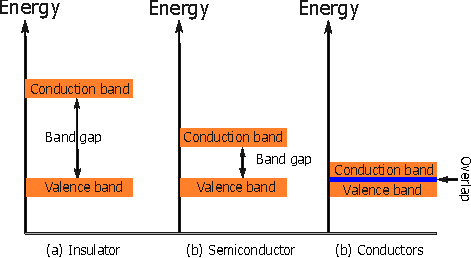
\includegraphics[width=0.8\textwidth]{fig/lec02/band_diagram.pdf}
                \caption{Energy band diagram showing the classification of materials}
            \end{figure}
\end{frame}

%%%%%%%%%%%%%%%%%%%%%%%%%%%%%%%%%%%%%%%%%%%%%%%%%%%%%%%%%%%%%
%% Energy Band diagram and classification  %%
%%%%%%%%%%%%%%%%%%%%%%%%%%%%%%%%%%%%%%%%%%%%%%%%%%%%%%%%%%%%%
\begin{frame}
	\frametitle{Energy band diagram and classification of materials}
    \begin{columns}
        \begin{column}{0.6\textwidth}
            \begin{itemize}
                \item Energy band diagram shows the energy levels of electrons in a solid material.
                \item The energy bands are separated by band gaps, which determine the electrical properties of the material.
                \item Materials can be classified based on their energy band structure:
                \begin{itemize}
                    \item Conductors: No band gap, electrons can move freely.
                    \item Semiconductors: Small band gap, electrons can be excited to the conduction band with some energy input.
                    \item Insulators: Large band gap, electrons cannot move freely without significant energy input.
                \end{itemize}
            \end{itemize}
    \end{column}
        \hfill
        \begin{column}{0.4\textwidth}
            \begin{figure}
                \centering
                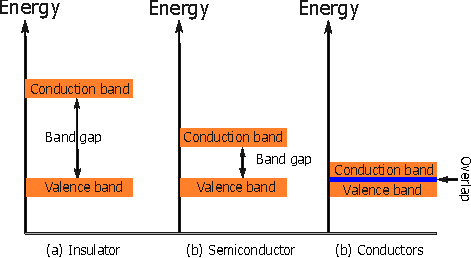
\includegraphics[width=0.8\textwidth]{fig/lec02/band_diagram.pdf}
                \caption{Energy band diagram showing the classification of materials}
            \end{figure}
        \end{column}
\end{columns}
\end{frame}

%%%%%%%%%%%%%%%%%%%%%%%%%%%%%%%%%%%%%%%%%%%%%%%%%%%%%%%%%%%%%
%% Conclusion on types of materials  %%
%%%%%%%%%%%%%%%%%%%%%%%%%%%%%%%%%%%%%%%%%%%%%%%%%%%%%%%%%%%%%
\begin{frame}
	\frametitle{Conclusion on types of materials}
    \begin{itemize}
    \item We learnt in two ways about classification of materials:
        \begin{itemize}
            \item Based on the number of valence electrons.
            \item Based on the energy band structure.
        \end{itemize}
    \end{itemize}
    \begin{columns}
        \begin{column}{0.6\textwidth}
            \begin{figure}
                \centering
                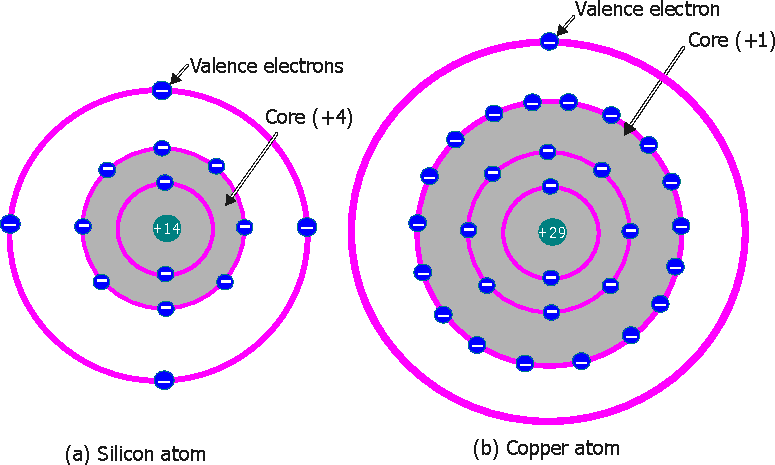
\includegraphics[width=0.6\textwidth]{fig/lec02/Cu_Si_atom1.pdf}
                \caption{(a) Silicon atom with four valence electrons, (b) Copper atom with one valence electron}
            \end{figure}
        \end{column}
        \hfill
        \begin{column}{0.4\textwidth}
            \begin{figure}
                \centering
                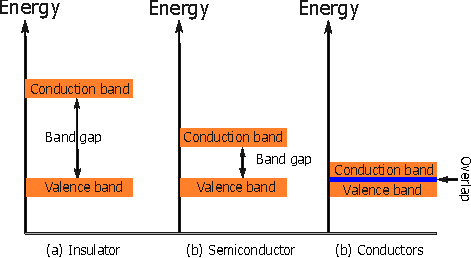
\includegraphics[width=0.6\textwidth]{fig/lec02/band_diagram.pdf}
                \caption{Energy band diagram showing the classification of materials}
            \end{figure}
        \end{column}
\end{columns}
\textbf{What next? $\rightarrow$ We will learn about the flow of electrons and holes in semiconductors.}
\end{frame}

%%%%%%%%%%%%%%%%%%%%%%%%%%%%%%%%%%%%%%%%%%%%%%%%%%%%%%%%%%%%%
%% Flow of current in semiconductors  %%
%%%%%%%%%%%%%%%%%%%%%%%%%%%%%%%%%%%%%%%%%%%%%%%%%%%%%%%%%%%%%
\begin{frame}
	\frametitle{Free electrons and holes in semiconductors}
            \begin{itemize}
                \item In semiconductors, the energy band gap is small enough that some electrons can be thermally excited from the valence band to the conduction band at room temperature.
                \item This process creates \textbf{free electrons} (also called \textbf{conduction electrons}) in the conduction band and \textbf{holes} (a vacant state that behaves like a positive charge) in the valence band.
                \item  Example: At room temperature, intrinsic silicon has enough thermal energy to excite some valence electrons across the band gap.
                \item This process results in \textbf{electron-hole pairs}.
                \item Free electrons and holes drift under electric fields and contribute to electrical conductivity.
                \item The concentration of free electrons and holes in a semiconductor can be controlled by doping with impurities.
            \end{itemize}
\end{frame}

%%%%%%%%%%%%%%%%%%%%%%%%%%%%%%%%%%%%%%%%%%%%%%%%%%%%%%%%%%%%%
%% Flow of electron current in semiconductors  %%
%%%%%%%%%%%%%%%%%%%%%%%%%%%%%%%%%%%%%%%%%%%%%%%%%%%%%%%%%%%%%
\begin{frame}
	\frametitle{Electron curent in semiconductors}
    \begin{figure}
        \centering
        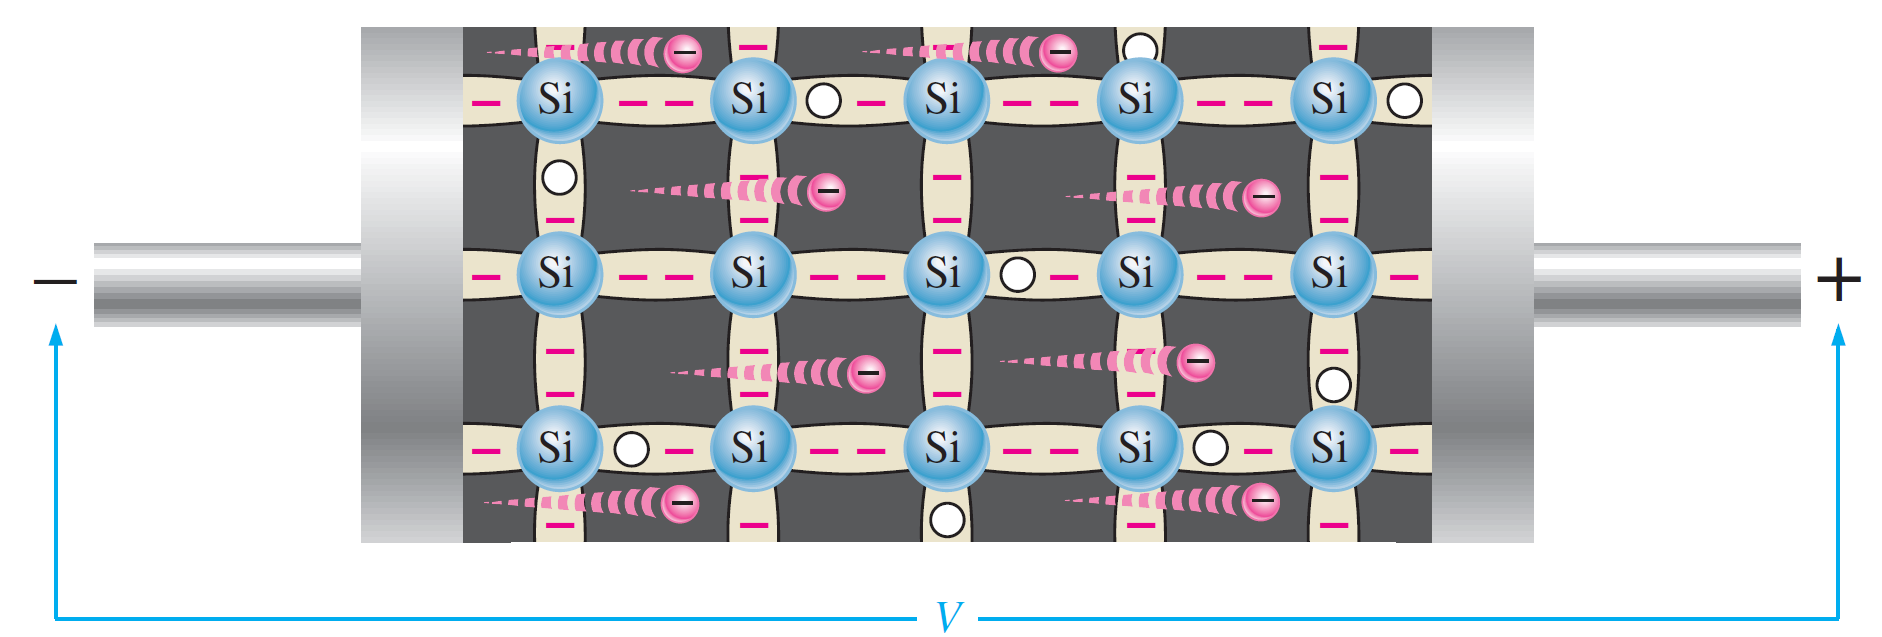
\includegraphics[width=0.75\textwidth]{fig/lec02/electron_current.png}
        \caption{Electron current in semiconductors (intrinsic Si) (Adapted from \href{https://www.pearson.com/en-us/subject-catalog/p/electronic-devices-electron-flow-version/P200000001048/9780137556755}{Electronic Devices (Electron Flow Version), 10th edition})}
    \end{figure}
    \textbf{The current we speak in general is the flow of electrons in a conductor. In semiconductors, the current is due to the flow of both electrons and holes.}
\end{frame}

%%%%%%%%%%%%%%%%%%%%%%%%%%%%%%%%%%%%%%%%%%%%%%%%%%%%%%%%%%%%%
%% Flow of hole current in semiconductors  %%
%%%%%%%%%%%%%%%%%%%%%%%%%%%%%%%%%%%%%%%%%%%%%%%%%%%%%%%%%%%%%
\begin{frame}
	\frametitle{Electron curent in semiconductors}
    \begin{figure}
        \centering
        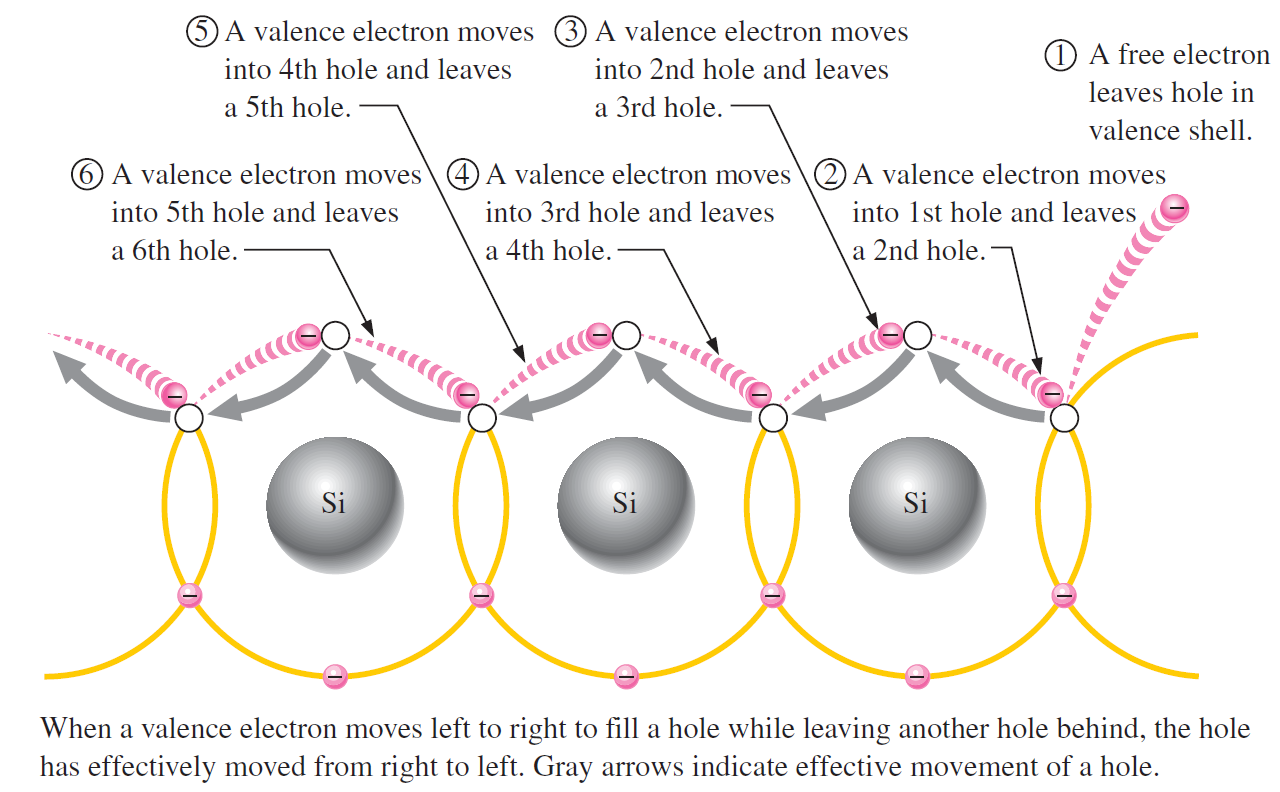
\includegraphics[width=0.65\textwidth]{fig/lec02/hole_current.png}
        \caption{Hole current in semiconductors (intrinsic Si) (Adapted from \href{https://www.pearson.com/en-us/subject-catalog/p/electronic-devices-electron-flow-version/P200000001048/9780137556755}{Electronic Devices (Electron Flow Version), 10th edition})}
    \end{figure}
\end{frame}

%%%%%%%%%%%%%%%%%%%%%%%%%%%%%%%%%%%%%%%%%%%%%%%%%%%%%%%%%%%%%
%% N-type and p-type semiconductor  %%
%%%%%%%%%%%%%%%%%%%%%%%%%%%%%%%%%%%%%%%%%%%%%%%%%%%%%%%%%%%%%
\begin{frame}
	\frametitle{N-type and P-type semiconductors}
    \begin{itemize}
        \item \textbf{Doping}: The process of adding impurities to a intrinsic (pure) semiconductor to change its electrical properties.
        \item N-type semiconductors are formed by doping intrinsic semiconductors with elements that have more valence electrons (e.g., phosphorus (P), arsenic (As)).
        \item In N-type semiconductors, the majority carriers are free electrons, while in P-type semiconductors, the majority carriers are holes.
        \item P-type semiconductors are formed by doping intrinsic semiconductors with elements that have fewer valence electrons (e.g., boron (B), gallium (Ga)).
        \item The minority carriers in N-type semiconductors are holes, while in P-type semiconductors, the minority carriers are free electrons.
    \end{itemize}
\end{frame}

%%%%%%%%%%%%%%%%%%%%%%%%%%%%%%%%%%%%%%%%%%%%%%%%%%%%%%%%%%%%%
%% Fundamental properties and terminologies  %%
%%%%%%%%%%%%%%%%%%%%%%%%%%%%%%%%%%%%%%%%%%%%%%%%%%%%%%%%%%%%%
\begin{frame}
	\frametitle{Understanding the doping process- \textbf{Donor} and Acceptor atoms}
    \begin{columns}
        \begin{column}{0.65\textwidth}
    \begin{itemize}
        \item \textbf{Donor atoms}: Atoms that donate extra electrons to the semiconductor lattice, creating N-type semiconductors.
        \item \textbf{Example of donor:} 
        \begin{itemize}
            \item Consider Germanium (Ge) as the intrinsic semiconductor. It is a group IV element with 4 valence electrons.
            \item When doped with Phosphorus (P), a group V element with 5 valence electrons, the extra electron from P becomes a free electron in the conduction band of Ge.
            \item This creates an N-type semiconductor with a higher concentration of free electrons than holes.
            \item The enrgy required to detach the extra electron from the donor atom is very small, so it is easily ionised at room temperature. For example, the ionisation energy of P in Ge is about 0.01 eV and for Si is about 0.045 eV.
        \end{itemize}    
    \end{itemize}
        \end{column}
        \hfill
        \begin{column}{0.35\textwidth}
            \begin{figure}
                \centering
                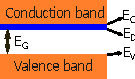
\includegraphics[scale=1.5]{fig/lec02/donor.pdf}
                \caption{Energy band diagram of an n-type semiconductor- allowable energy levels introduced in the conduction band. $E_D$ is also called Fermi level ($E_F$).}
            \end{figure}
    \end{column}
        \end{columns}
\end{frame}

%%%%%%%%%%%%%%%%%%%%%%%%%%%%%%%%%%%%%%%%%%%%%%%%%%%%%%%%%%%%%
%% Fundamental properties and terminologies  %%
%%%%%%%%%%%%%%%%%%%%%%%%%%%%%%%%%%%%%%%%%%%%%%%%%%%%%%%%%%%%%
\begin{frame}
	\frametitle{Understanding the doping process- Donor and \textbf{Acceptor atoms}}
    \begin{columns}
        \begin{column}{0.65\textwidth}
    \begin{itemize}
        \item \textbf{Acceptor atoms}: Atoms that accept electrons from the semiconductor lattice, creating P-type semiconductors.
        \item \textbf{Example of Acceptor:} 
        \begin{itemize}
            \item Consider Silicon (Si) as the intrinsic semiconductor. It is a group IV element with 4 valence electrons.
            \item When doped with Boron (B), a group III element with 3 valence electrons, the missing electron from B creates a hole in the valence band of Si.
            \item This creates a P-type semiconductor with a higher concentration of holes than free electrons.
            \item The energy required to fill the hole is very small, so it is easily ionised at room temperature. For example, the ionisation energy of B in Si is about 0.045 eV and for Ga is about 0.1 eV.
        \end{itemize}
    \end{itemize}
    \end{column}
    \hfill
    \begin{column}{0.35\textwidth}
        \begin{figure}
            \centering
            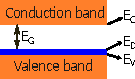
\includegraphics[scale=1.5]{fig/lec02/acceptor.pdf}
            \caption{Energy band diagram of an p-type semiconductor- allowable energy levels introduced in the valence band.  $E_D$ is also called Fermi level ($E_F$)}
        \end{figure}
    \end{column}
    \end{columns}
\end{frame}
%%%%%%%%%%%%%%%%%%%%%%%%%%%%%%%%%%%%%%%%%%%%%%%%%%%%%%%%%%%%%
%% The pn junction in a semiconductor  %%
%%%%%%%%%%%%%%%%%%%%%%%%%%%%%%%%%%%%%%%%%%%%%%%%%%%%%%%%%%%%%
\begin{frame}
	\frametitle{Acceptor and donor atoms in a semiconductor- example}
    \begin{columns}
        \begin{column}{0.5\textwidth}
            \begin{figure}
                \centering
                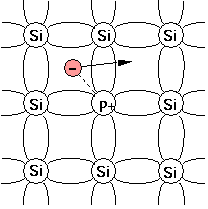
\includegraphics[scale=0.5]{fig/lec02/Donor_in_Si_lattice.png}
                \caption{Phosphorus atom acting as a donor in the simplified 2D silicon lattice. (Source: from \href{https://commons.wikimedia.org/wiki/File:Donor_in_Si_lattice.png}{Karolkalna at the English Wikipedia}, \href{http://creativecommons.org/licenses/by-sa/3.0/}{CC BY-SA 3.0})}
            \end{figure}
    \end{column}
    \hfill
    \begin{column}{0.5\textwidth}
        \begin{figure}
            \centering
            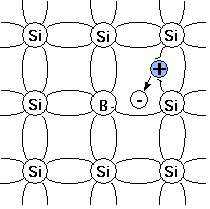
\includegraphics[scale=0.5]{fig/lec02/Acceptor_in_Si_lattice.png}
            \caption{Boron atom acting as an acceptor in the simplified 2D silicon lattice- (Source: from \href{https://commons.wikimedia.org/wiki/File:Acceptor_in_Si_lattice.png}{Karolkalna at the English Wikipedia}, \href{http://creativecommons.org/licenses/by-sa/3.0/}{CC BY-SA 3.0})}
        \end{figure}
    \end{column}
    \end{columns}
\end{frame}

%%%%%%%%%%%%%%%%%%%%%%%%%%%%%%%%%%%%%%%%%%%%%%%%%%%%%%%%%%%%%
%% Mass action law%%
%%%%%%%%%%%%%%%%%%%%%%%%%%%%%%%%%%%%%%%%%%%%%%%%%%%%%%%%%%%%%
\begin{frame}
    \frametitle{Mass action law}
    \begin{itemize}
        \item The mass action law states that the product of the concentrations of electrons and holes in a semiconductor is constant at a given temperature.
        \item This relationship can be expressed mathematically as:
        \begin{equation}
            n \cdot p = n_i^2
        \end{equation}
        where $n$ is the concentration of free electrons, $p$ is the concentration of holes, and $n_i$ is the intrinsic carrier concentration.
        \item The intrinsic carrier concentration ($n_i$) is a measure of the number of electron-hole pairs generated in an intrinsic semiconductor at thermal equilibrium.
    \end{itemize}
\end{frame}

%%%%%%%%%%%%%%%%%%%%%%%%%%%%%%%%%%%%%%%%%%%%%%%%%%%%%%%%%%%%%
% Charge Neutrality and n-Type Case
%%%%%%%%%%%%%%%%%%%%%%%%%%%%%%%%%%%%%%%%%%%%%%%%%%%%%%%%%%%%%
\begin{frame}{Charge Neutrality in Semiconductors}
    \begin{itemize}
        \item Electrical neutrality:
        \begin{equation}
        N_D + p = N_A + n 
        \end{equation}
        \item For \textbf{n-type material} ($N_A = 0$):
        \begin{equation}
        n \approx N_D 
        \end{equation}
        \item Thus, free-electron concentration equals donor atom concentration.
        \item More clearly written with subscripts:
        \begin{equation} \label{eq:charge_neutrality_n}
        n_n \approx N_D 
        \end{equation}
        \item Hole concentration:
        \begin{equation} \label{eq:charge_neutrality_p}
        p_n = \frac{n_i^2}{N_D} 
        \end{equation}
    \end{itemize}
\end{frame}
%%%%%%%%%%%%%%%%%%%%%%%%%%%%%%%%%%%%%%%%%%%%%%%%%%%%%%%%%%%%%
% p-Type Case and Doping Balance
%%%%%%%%%%%%%%%%%%%%%%%%%%%%%%%%%%%%%%%%%%%%%%%%%%%%%%%%%%%%%
\begin{frame}{p-Type Semiconductors and Doping}
    \begin{itemize}
        \item For \textbf{p-type semiconductors}:
        \begin{equation}
        p_p \approx N_A, \quad n_p = \frac{n_i^2}{N_A}
        \end{equation}
        \item Equal donor and acceptor concentrations ($N_D = N_A$) $\Rightarrow$ intrinsic behavior.
        \item Doping can switch material type depending on relative $N_D$ and $N_A$.
        \item For $N_D > N_A$, p-type becomes n-type.
        \item Adjusted neutrality (general case):
        \begin{equation}
        N_D + p = N_A + n \Rightarrow N_D - N_A = n - p
        \end{equation}
        %\item Modify Eqs. (\ref{eq:charge_neutrality_n}) and (\ref{eq:charge_neutrality_p}): Replace $N_D$ with $N_D - N_A$
    \end{itemize}
\end{frame}
%%%%%%%%%%%%%%%%%%%%%%%%%%%%%%%%%%%%%%%%%%%%%%%%%%%%%%%%%%%%%
% Conductivity in Semiconductors
%%%%%%%%%%%%%%%%%%%%%%%%%%%%%%%%%%%%%%%%%%%%%%%%%%%%%%%%%%%%%
\begin{frame}{Conductivity and Carrier Mobility}
    \begin{itemize}
        \item Semiconductors are \textbf{bipolar}: conduction via both electrons and holes.
        \item Current density:
        \begin{equation}
        J = (n \mu_n + p \mu_p)q\mathcal{E} = \sigma \mathcal{E} \tag{2-16}
        \end{equation}
        \item $n$, $p$: carrier concentrations; $\mu_n$, $\mu_p$: mobilities.
        \item Conductivity:
        \begin{equation}
        \sigma = (n \mu_n + p \mu_p)q \tag{2-17}
        \end{equation}
        \item Intrinsic case: $n = p = n_i$
    \end{itemize}
\end{frame}

%%%%%%%%%%%%%%%%%%%%%%%%%%%%%%%%%%%%%%%%%%%%%%%%%%%%%%%%%%%%%
% Temperature Dependence of Intrinsic Carriers
%%%%%%%%%%%%%%%%%%%%%%%%%%%%%%%%%%%%%%%%%%%%%%%%%%%%%%%%%%%%%
\begin{frame}{Intrinsic Carrier Concentration and Temperature Dependence}
    \begin{itemize}
        \item As temperature increases, intrinsic carrier concentration increases:
        \begin{equation}
        n_i^2 = A_0 T^3 e^{-E_{G0}/kT} \tag{2-18}
        \end{equation}
        \item Temperature-dependent bandgap:
        \begin{equation}
        E_G(T) = 1.21 - 3.60 \times 10^{-4}T \quad \text{(Si)} \tag{2-19}
        \end{equation}
        \begin{equation}
        E_G(T) = 0.785 - 2.23 \times 10^{-4}T \quad \text{(Ge)} \tag{2-20}
        \end{equation}
        \item As $T$ increases:
        \begin{itemize}
            \item $E_G$ decreases
            \item $n_i$ increases
            \item Conductivity increases
        \end{itemize}
    \end{itemize}
\end{frame}


%%%%%%%%%%%%%%%%%%%%%%%%%%%%%%%%%%%%%%%%%%%%%%%%%%%%%%%%%%%%%
% The Hall Effect - Introduction
%%%%%%%%%%%%%%%%%%%%%%%%%%%%%%%%%%%%%%%%%%%%%%%%%%%%%%%%%%%%%
\begin{frame}{The Hall Effect}
\begin{columns}
    \begin{column}{0.5\textwidth}
    \begin{itemize}
        \item When a semiconductor carries a current $I$ in a transverse magnetic field $B$, an electric field $\mathcal{E}$ develops perpendicular to both $I$ and $B$.
        \item This phenomenon is known as the \textbf{Hall Effect}.
        \item Used to determine:
        \begin{itemize}
            \item Whether a semiconductor is \textbf{n-type} or \textbf{p-type}
            \item The carrier concentration
            \item The mobility $\mu$ of carriers
        \end{itemize}
        \item A potential difference, called the \textbf{Hall voltage} $V_H$, appears across the sample.
    \end{itemize}
\end{column}
\begin{column}{0.5\textwidth}
    \begin{figure}[h]
        \centering
        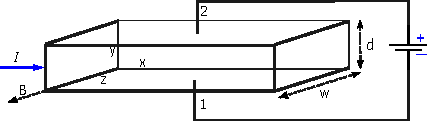
\includegraphics[width=1\textwidth]{fig/lec02/hall_effect.pdf} % Replace with your actual image file
        \caption{Schematic diagram of Hall setup showing force on charge carriers}
    \end{figure}
\end{column}
\end{columns}
\end{frame}

%%%%%%%%%%%%%%%%%%%%%%%%%%%%%%%%%%%%%%%%%%%%%%%%%%%%%%%%%%%%%
% Hall Effect - Physical Explanation
%%%%%%%%%%%%%%%%%%%%%%%%%%%%%%%%%%%%%%%%%%%%%%%%%%%%%%%%%%%%%
\begin{frame}{Lorentz Force and Hall Field}
    \begin{itemize}
        \item Consider a semiconductor sample placed in a magnetic field $\vec{B}$ in the $z$-direction.
        \item A current $I$ is passed in the $x$-direction, perpendicular to $\vec{B}$.
        \item Charge carriers (electrons or holes) moving with velocity $\vec{v}$ experience a force:
        \begin{equation}
        \vec{F} = q(\vec{v} \times \vec{B})
        \end{equation}
        \item This Lorentz force deflects carriers in the $+y$ direction, creating:
        \begin{itemize}
            \item Negative charge on the $+y$ side (if electrons dominate)
            \item Positive charge on the $-y$ side
        \end{itemize}
        \item This generates an electric field $E_H$ opposing the Lorentz force:
        \begin{equation} \label{eq:Lorentz_force}
        \vec{F} = q(\vec{E} + \vec{v} \times \vec{B}) = 0 
        \end{equation}
        For simplicity, let's represent $\vec{E}=\mathcal{E}$
    \end{itemize}
\end{frame}

%%%%%%%%%%%%%%%%%%%%%%%%%%%%%%%%%%%%%%%%%%%%%%%%%%%%%%%%%%%%%
% Hall Field and Charge Type Identification
%%%%%%%%%%%%%%%%%%%%%%%%%%%%%%%%%%%%%%%%%%%%%%%%%%%%%%%%%%%%%
\begin{frame}{Hall Voltage and Carrier Type}
    \begin{itemize}
        \item Solving Eq. \ref{eq:Lorentz_force} gives the Hall field:
        \begin{equation}
            \mathcal{E} = v_x B_z 
        \end{equation}
        \item This field gives rise to a Hall voltage:
        \begin{equation}
        V_H = d \mathcal{E} = d v_x B_z
        \end{equation}
        \item $d$: width of the semiconductor sample
        \item Since current $I \propto q v_x$, the sign of $V_H$ indicates:
        \begin{itemize}
            \item $V_H > 0$: Majority carriers are electrons (n-type)
            \item $V_H < 0$: Majority carriers are holes (p-type)
        \end{itemize}
        \item Thus, \textbf{Hall effect enables determination of carrier type} in semiconductors
    \end{itemize}
\end{frame}

%%%%%%%%%%%%%%%%%%%%%%%%%%%%%%%%%%%%%%%%%%%%%%%%%%%%%%%%%%%%%
% Derivation of Hall Voltage
%%%%%%%%%%%%%%%%%%%%%%%%%%%%%%%%%%%%%%%%%%%%%%%%%%%%%%%%%%%%%

\begin{frame}{Experimental Determination of $\mu$ (mobility of charge carrier) and $\rho$ (charge density)}
    \begin{itemize}
        \item In the equilibrium state the electric field intensity $\mathcal{E}$ due to Hall effect must be equal to the magnetic force:
        \begin{equation}
        q\mathcal{E} = Bqv \tag{2-21}
        \end{equation}
        \item Using $\mathcal{E} = \frac{V_H}{d}$ and $J = \rho v = \frac{I}{wd}$, where $\rho$ is the charge density, $w$ is the width of the sample, and $J$ is the current density:
        \begin{equation}
        V_H = \mathcal{E}d = Bvd = \frac{BJd}{\rho} = \frac{BI}{\rho w} \tag{2-22}
        \end{equation}
        \item Hence $\rho$ can be expressed as:
        \begin{equation}
        \rho = \frac{BI}{V_H w} \Rightarrow R_H = \frac{1}{\rho} = \frac{V_H w}{BI} \tag{2-23, 2-24}
        \end{equation}
        where $R_H$ is the Hall coefficient.
    \end{itemize}
\end{frame}

%%%%%%%%%%%%%%%%%%%%%%%%%%%%%%%%%%%%%%%%%%%%%%%%%%%%%%%%%%%%%
% Mobility from Hall Coefficient
%%%%%%%%%%%%%%%%%%%%%%%%%%%%%%%%%%%%%%%%%%%%%%%%%%%%%%%%%%%%%
\begin{frame}{Hall Coefficient and Mobility}
    \begin{itemize}
        \item Conductivity: $\sigma = \rho \mu$ (for single carrier type)
        \item Therefore, mobility:
        \begin{equation}
        \mu = \sigma R_H \tag{2-26}
        \end{equation}
        \item If random thermal motion is accounted for:
        \begin{equation}
        \mu = \left( \frac{8\sigma}{3\pi} \right) R_H
        \end{equation}
        \item Hall effect allows complete characterization of a semiconductor.
    \end{itemize}
\end{frame}

%%%%%%%%%%%%%%%%%%%%%%%%%%%%%%%%%%%%%%%%%%%%%%%%%%%%%%%%%%%%%
% Applications and Conductivity Modulation
%%%%%%%%%%%%%%%%%%%%%%%%%%%%%%%%%%%%%%%%%%%%%%%%%%%%%%%%%%%%%
\begin{frame}{Applications and Conductivity Modulation}
    \begin{itemize}
        \item Applications:
        \begin{itemize}
            \item Magnetic field sensors (Hall-effect meters)
            \item Hall-effect multipliers (measure product of two signals)
        \end{itemize}
        \item Conductivity $\sigma$ can be modulated by:
        \begin{itemize}
            \item Varying temperature
            \item Doping to increase $n$ or $p$
            \item Illumination to generate electron-hole pairs
        \end{itemize}
        \item Reiterates Eq. (2-17): $\sigma = (n\mu_n + p\mu_p)q$
    \end{itemize}
\end{frame}

%%%%%%%%%%%%%%%%%%%%%%%%%%%%%%%%%%%%%%%%%%%%%%%%%%%%%%%%%%%%%
% Carrier Generation and Recombination
%%%%%%%%%%%%%%%%%%%%%%%%%%%%%%%%%%%%%%%%%%%%%%%%%%%%%%%%%%%%%

\begin{frame}{Carrier Generation and Recombination}

    \begin{itemize}
        \item \textbf{Generation}: Creation of electron-hole pairs (EHPs)
        \begin{itemize}
            \item Due to thermal energy or light (photons)
        \end{itemize}
        \item \textbf{Recombination}: Annihilation of an electron with a hole
        \item At equilibrium, generation rate $G$ equals recombination rate $R$
        \item Important for determining carrier lifetime $\tau$: Average time a carrier exists before recombination.
        \item \textbf{Auger recombination}: Involves three carriers (two electrons and one hole or vice versa). 
        \begin{itemize}
            \item It it transfer of the energy and momentum released by the recombination of an electron-hole pair to a third mobile particle- electrons in the case of heavily doped N-type material and holes in the case of heavily doped P-type material.
            \item It is a non-radiative process and is the dominant recombination mechanism in heavily doped semiconductors.
            \item Auger recombination is a significant factor in determining the efficiency of semiconductor devices, especially in \textbf{high-power and high-frequency applications}.
        \end{itemize}
        \item \textbf{Radiative recombination}: Involves emission of a photon.
    \end{itemize}

\end{frame}

%%%%%%%%%%%%%%%%%%%%%%%%%%%%%%%%%%%%%%%%%%%%%%%%%%%%%%%%%%%%%
% Carrier Diffusion
%%%%%%%%%%%%%%%%%%%%%%%%%%%%%%%%%%%%%%%%%%%%%%%%%%%%%%%%%%%%%

\begin{frame}{Carrier Diffusion}
    \begin{itemize}
        \item Caused by spatial concentration gradients of charge carriers
        \item Electrons and holes move from regions of high to low concentration
        \item Electron diffusion current density:
        \begin{equation}
        J_n^{\text{diff}} = q D_n \frac{dn}{dx}
        \end{equation}
        \item Hole diffusion current density:
        \begin{equation}
        J_p^{\text{diff}} = -q D_p \frac{dp}{dx}
        \end{equation}
        \item Where:
        \begin{itemize}
            \item $q$: elementary charge
            \item $D_n$, $D_p$: diffusion coefficients of electrons and holes
            \item $\frac{dn}{dx}$, $\frac{dp}{dx}$: gradients of electron and hole concentrations with respect to position $x$
        \end{itemize}
    \end{itemize}
\end{frame}

%%%%%%%%%%%%%%%%%%%%%%%%%%%%%%%%%%%%%%%%%%%%%%%%%%%%%%%%%%%%%
% Carrier Drift
%%%%%%%%%%%%%%%%%%%%%%%%%%%%%%%%%%%%%%%%%%%%%%%%%%%%%%%%%%%%%
\begin{frame}{Carrier Drift}
    \begin{itemize}
        \item Caused by an applied electric field $\mathcal{E}$ across the semiconductor
        \item Electron drift current:
        \begin{equation}
        J_n^{\text{drift}} = q n \mu_n \mathcal{E}
        \end{equation}
        \item Hole drift current:
        \begin{equation}
        J_p^{\text{drift}} = q p \mu_p \mathcal{E}
        \end{equation}
        \item Where:
        \begin{itemize}
            \item $n$, $p$: concentrations of electrons and holes
            \item $\mu_n$, $\mu_p$: mobilities of electrons and holes
            \item $\mathcal{E}$: electric field (V/m)
        \end{itemize}
        \item Drift current is proportional to the electric field and carrier concentration
        \item Drift and diffusion currents are the two main mechanisms of charge transport in semiconductors
    \end{itemize}
\end{frame}



%%%%%%%%%%%%%%%%%%%%%%%%%%%%%%%%%%%%%%%%%%%%%%%%%%%%%%%%%%%%%
% Drift vs Diffusion
%%%%%%%%%%%%%%%%%%%%%%%%%%%%%%%%%%%%%%%%%%%%%%%%%%%%%%%%%%%%%
\begin{frame}{Distinction: Drift vs Diffusion Currents}
    \centering
    \textbf{Comparison of Drift and Diffusion Currents} \\[1ex]
    \begin{tabular}{|p{3cm}|p{4cm}|p{4cm}|}
        \hline
        \textbf{Aspect} & \textbf{Drift Current} & \textbf{Diffusion Current} \\
        \hline
        Driving Force & Electric field ($\mathcal{E}$) & Concentration gradient ($\frac{dn}{dx}$ or $\frac{dp}{dx}$) \\
        \hline
        Direction & Field direction & High to low concentration \\
        \hline
        Equation & $q n \mu \mathcal{E}$ or $q p \mu \mathcal{E}$ & $q D \frac{dn}{dx}$ or $-q D \frac{dp}{dx}$ \\
        \hline
        Occurs Due To & External bias & Inhomogeneous doping or illumination \\
        \hline
        Field Requirement & Required & Not required \\
        \hline
    \end{tabular}
\end{frame}

%%%%%%%%%%%%%%%%%%%%%%%%%%%%%%%%%%%%%%%%%%%%%%%%%%%%%%%%%%%%%
% RElating mobility and diffusion of charge carriers
%%%%%%%%%%%%%%%%%%%%%%%%%%%%%%%%%%%%%%%%%%%%%%%%%%%%%%%%%%%%%
\begin{frame}{How mobility and diffusion are related of charge carrier are related?}
    \begin{itemize}
        \item \textbf{Mobility} ($\mu$): Measure of how quickly charge carriers (electrons or holes) can move through a semiconductor material in response to an electric field.
        \item \textbf{Diffusion coefficient} ($D$): Measure of how quickly charge carriers can spread out in a semiconductor material due to concentration gradients.
        \item \textbf{Einstein relation}: Connects mobility and diffusion coefficient:
        \begin{equation}
        D = \frac{kT}{q} \mu    
        \end{equation}
        \item Where:
        \begin{itemize}
            \item $k$: Boltzmann constant
            \item $T$: Absolute temperature (in Kelvin)
            \item $q$: Elementary charge (charge of an electron)
        \end{itemize}
        \item This relation shows that the diffusion coefficient is directly proportional to the mobility of charge carriers and the temperature.
        \item Higher mobility leads to higher diffusion rates, which is important for understanding charge transport in semiconductors.
    \end{itemize}
    \end{frame}

    %%%%%%%%%%%%%%%%%%%%%%%%%%%%%%%%%%%%%%%%%%%%%%%%%%%%%%%%%%%%%
% RElating mobility and diffusion of charge carriers
%%%%%%%%%%%%%%%%%%%%%%%%%%%%%%%%%%%%%%%%%%%%%%%%%%%%%%%%%%%%%
\begin{frame}{Relevance of Einstein relation?}
    \begin{itemize}
        \item The Einstein relation is a fundamental concept that bridge the microscopic thermal motion of carriers with their macroscopic electrical behavior, and is essential for modeling how semiconductors behave under various conditions.
        \item \textbf{Unifies Drift and Diffusion:} Shows that mobility (drift due to electric field) and diffusion (due to concentration gradient) are inherently linked by thermal motion.
        \item \textbf{Device Modeling:} Essential for modeling carrier transport in semiconductors such as diodes, BJTs, and MOSFETs where both drift and diffusion processes coexist.
        \item \textbf{Simplifies Analysis:} If one parameter (e.g., mobility) is known, diffusion coefficient can be calculated, reducing experimental complexity.
        \item \textbf{Temperature Dependence:} Since $D \propto T$ and $\mu \propto T^{-m}$ (where $m \approx 1.5$), the Einstein relation captures how transport properties change with temperature — crucial for thermal sensor and reliability design.
        \item \textbf{Measurement and Material Characterization:} Enables calculation of diffusion coefficient $D$ from mobility $\mu$ measured using Hall effect.
    \end{itemize}
\end{frame}

%%%%%%%%%%%%%%%%%%%%%%%%%%%%%%%%%%%%%%%%%%%%%%%%%%%%%%%%%%%%%
% Deriving the Einstein Relation
%%%%%%%%%%%%%%%%%%%%%%%%%%%%%%%%%%%%%%%%%%%%%%%%%%%%%%%%%%%%%
\begin{frame}{Deriving Einstein Relation}
    \begin{itemize}
        \item The Einstein relation connects the diffusion coefficient ($D$) and the mobility ($\mu$) of charge carriers in thermal equilibrium.
        \item For electrons:
        \begin{equation}
        D_n = \frac{kT}{q} \mu_n, \quad \text{and for holes: } D_p = \frac{kT}{q} \mu_p
        \end{equation}
        \item \textbf{Start with the drift current:} 
        \begin{equation}
        J_n^{\text{drift}} = q n \mu_n \mathcal{E}
        \end{equation}
        \item \textbf{In equilibrium}, the total electron current must be zero:
        \begin{equation}
        J_n^{\text{drift}} + J_n^{\text{diff}} = 0
        \Rightarrow q n \mu_n \mathcal{E} + q D_n \frac{dn}{dx} = 0
        \end{equation}
    \end{itemize}
\end{frame}

\begin{frame}{Deriving Einstein Relation. Contd.}
    \begin{itemize}
        \item From Boltzmann distribution:
        \begin{equation}
        n(x) \propto e^{-q\phi(x)/kT} \Rightarrow \frac{dn}{dx} = \frac{q n \mathcal{E}}{kT}
        \end{equation}
        \item Substituting back into current balance:
        \begin{align*}
        q n \mu_n \mathcal{E} + q D_n \left( \frac{q n \mathcal{E}}{kT} \right) &= 0 \\
        \Rightarrow q n \mathcal{E} \left( \mu_n + \frac{q D_n}{kT} \right) &= 0
        \end{align*}
        \item Since $q n \mathcal{E} \neq 0$ in general, we get:
        \begin{equation}
        D_n = \frac{kT}{q} \mu_n
        \end{equation}
        \item Similarly, for holes:
        \begin{equation}
        D_p = \frac{kT}{q} \mu_p
        \end{equation}
    \end{itemize}
\end{frame}

%%%%%%%%%%%%%%%%%%%%%%%%%%%%%%%%%%%%%%%%%%%%%%%%%%%%%%%%%%%%%
% Continuity Equation
%%%%%%%%%%%%%%%%%%%%%%%%%%%%%%%%%%%%%%%%%%%%%%%%%%%%%%%%%%%%%
\begin{frame}{Continuity Equation}
    \begin{itemize}
        \item Expresses conservation of charge carriers over time and space and ensured that the total charge in a semiconductor remains constant or the law of \textbf{conservation of charge}.
        \item For electrons:
        \begin{equation}
        \frac{\partial n}{\partial t} = \frac{1}{q} \frac{\partial J_n}{\partial x} + G_n - R_n
        \end{equation}
        \item Where:
        \begin{itemize}
            \item $n$: electron concentration (per unit volume)
            \item $J_n$: electron current density
            \item $G_n$: electron generation rate
            \item $R_n$: electron recombination rate
        \end{itemize}
        \item Similar form exists for holes
        \item Important in analyzing transient or steady-state carrier dynamics
    \end{itemize}
\end{frame}

%%%%%%%%%%%%%%%%%%%%%%%%%%%%%%%%%%%%%%%%%%%%%%%%%%%%%%%%%%%%%
% Continuity Equation
%%%%%%%%%%%%%%%%%%%%%%%%%%%%%%%%%%%%%%%%%%%%%%%%%%%%%%%%%%%%%
\begin{frame}{Continuity Equation- relevance}
    \begin{itemize}
        \item Models \textbf{transient behavior} in devices (e.g., switching in transistors, photodiode response), basically how quickly a device responds to changes in input.
        \item Describes \textbf{steady-state operation} when $\partial n/\partial t = 0$, hence used in diode forward and reverse bias analysis, minority carrier injection in BJTs.
        \item Forms the backbone of \textbf{minority carrier analysis} in diodes and BJTs
        \item Extends to holes: \( \frac{\partial p}{\partial t} = -\frac{1}{q} \frac{\partial J_p}{\partial x} + G_p - R_p \), together with the electron equation, allows for a complete description of carrier dynamics in semiconductors.
        \item Couples with Poisson’s equation (describes how the electric potential varies in space due to the presence of electric charge within the material) for \textbf{complete device modeling} 
        \item Core equation in numerical tools like TCAD, COMSOL, Silvaco
    \end{itemize}
\end{frame}

%%%%%%%%%%%%%%%%%%%%%%%%%%%%%%%%%%%%%%%%%%%%%%%%%%%%%%%%%%%%%
% Impact Ionisation and Avalanche Breakdown
%%%%%%%%%%%%%%%%%%%%%%%%%%%%%%%%%%%%%%%%%%%%%%%%%%%%%%%%%%%%%
\begin{frame}{Impact Ionization}
    \begin{itemize}
        \item \textbf{Impact ionization}: Process where a high-energy electron collides with an atom, creating an electron-hole pair.
        \item This process can lead to a chain reaction, where the newly created electrons also gain enough energy to create more electron-hole pairs.
        \item Impact ionization is a high-field carrier generation mechanism leading to \textbf{avalanche multiplication}.
        \item It occurs when electrons or holes in a strong electric field gain sufficient kinetic energy to ionize atoms, creating electron-hole pairs.
        \item Fundamental in determining the \textbf{breakdown voltage} in devices like diodes and power MOSFETs.
        \item Before we proceed, just a short thought on how a device conducts current.
            \begin{itemize}
                \item In forward bias, due to diffusion of majority carriers, the depletion region shrinks and the current increases exponentially with voltage.
                \item In reverse bias, If voltage is low and doping is high $\rightarrow$ Zener breakdown, \\
                If voltage is high and doping is low $\rightarrow$ Avalanche breakdown
            \end{itemize}
    \end{itemize}
\end{frame}     % Physics of basic semiconductor devices
\section{p-n junctions and diodes}
\title{p-n junctions and diodes}  

\begin{frame}[plain]
    \titlepage
\end{frame}

%%%%%%%%%%%%%%%%%%%%%%%%%%%%%%%%%%%%%%%%%%%%%%%%%%%%%%%%%%%%%
%% Introduction to the p-n junctions %%
%%%%%%%%%%%%%%%%%%%%%%%%%%%%%%%%%%%%%%%%%%%%%%%%%%%%%%%%%%%%%
\begin{frame}
    \frametitle{What have you learnt and what you will learn?}

	\begin{itemize}
		\item WHat you have learnt so far? 
		\begin{itemize}
			\item How do a material behave as a conductor, semiconductor and insulator?
			\item How the current flows in a semiconductor?
			\item Mathematics of the current flow in a semiconductor?
			\item Proerpties of a intrinsic and extrinsic semiconductors?
			\item What is doping and \textbf{individual properties of n-type and p-type semiconductors?}
	\end{itemize}
		\item What you will learn in this lecture?
	\begin{itemize}
		\item What is a p-n junction? \textbf{How n-type and p-type semiconductors work together?}
		\item What is the depletion region?
		\item What is the built-in potential?
		\item What is the forward and reverse bias?
		\item What is the current-voltage characteristics of a diode?
		\item What are the different types of diodes?
		\item What are the applications of diodes?
	\end{itemize}
\end{itemize}
\end{frame}

%%%%%%%%%%%%%%%%%%%%%%%%%%%%%%%%%%%%%%%%%%%%%%%%%%%%%%%%%%%%%
%% Band diagrams of p-n junction %%
%%%%%%%%%%%%%%%%%%%%%%%%%%%%%%%%%%%%%%%%%%%%%%%%%%%%%%%%%%%%%
\begin{frame}
    \frametitle{Band diagrams of p-n junctions}
	\begin{itemize}
		\item A p-n junction is formed when a p-type semiconductor and an n-type semiconductor are brought into contact.
		\item The energy band diagrams of a p-n junction can be represented as follows:
		\begin{itemize}
			\item Before contact: The energy bands of the p-type and n-type semiconductors are separate.
			\item After contact: The energy bands of the p-n junction align, creating a depletion or space charge region at the interface.
			\item The conduction band and valence band of the n-type semiconductor are higher in energy than those of the p-type semiconductor.
			\item The Fermi level of the n-type semiconductor is higher than that of the p-type semiconductor before contact.
			\item After contact, the Fermi level becomes constant across the junction, indicating thermal equilibrium.
		\end{itemize}
		\item The energy band diagram of a p-n junction can be represented as follows:
\end{itemize}
\end{frame}


%%%%%%%%%%%%%%%%%%%%%%%%%%%%%%%%%%%%%%%%%%%%%%%%%%%%%%%%%%%%%
%% Band diagrams of p-n junction %%
%%%%%%%%%%%%%%%%%%%%%%%%%%%%%%%%%%%%%%%%%%%%%%%%%%%%%%%%%%%%%
\begin{frame}
    \frametitle{Band diagrams of p-n junctions}
	\begin{figure}
		\centering
		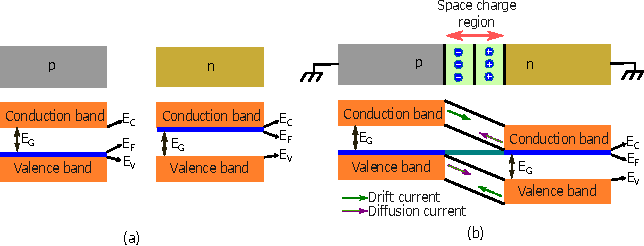
\includegraphics[width=0.8\textwidth]{fig/lec03/Band_diagram_all.pdf}
		\caption{Energy band diagram of a (a) discrete p and n (b) p-n junction.}
		\label{fig:pn_junction_all}
	\end{figure}
	\vspace{-0.5cm}
	\begin{itemize}
		\item The energy band diagram of a p-n junction shows the conduction band, valence band, and Fermi level of both the p-type and n-type semiconductors before and after contact.
		\item The depletion region is formed at the interface, where the majority carriers (holes in p-type and electrons in n-type) recombine, creating a region with no free charge carriers.
	\end{itemize}
\end{frame}


%%%%%%%%%%%%%%%%%%%%%%%%%%%%%%%%%%%%%%%%%%%%%%%%%%%%%%%%%%%%%
%% Band diagrams of p-n junction %%
%%%%%%%%%%%%%%%%%%%%%%%%%%%%%%%%%%%%%%%%%%%%%%%%%%%%%%%%%%%%%
\begin{frame}
	\frametitle{Band diagrams of p-n junctions}
	\begin{columns}
		\begin{column}{0.35\textwidth}
			\begin{itemize}
				\item \textbf{Step 1: Diffusion Due to Concentration Gradient}
				\begin{itemize}
					\item p-side: High hole concentration
					\item n-side: High electron concentration
					\item Result: Holes diffuse from p to n, electrons from n to p
				\end{itemize}
				\item \textbf{Step 2: Ions Left Behind → Space Charge}
				\begin{itemize}
					\item As mobile carriers leave, fixed ionized dopants remain:
					\begin{itemize}
						\item Negative acceptor ions in the p-region
						\item Positive donor ions in the n-region
					\end{itemize}
				\end{itemize}
			\end{itemize}
		\end{column}
		\begin{column}{0.7\textwidth}
			\begin{figure}
				\centering
				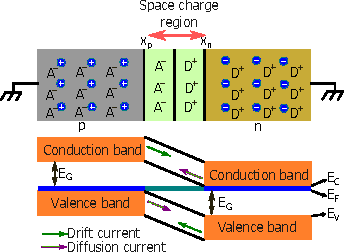
\includegraphics[scale=1.5]{fig/lec03/band_diagram_pn_junction_big.pdf}
				\caption{Energy band diagram of a p-n junction.}
				\label{fig:pn_junction}
			\end{figure}
		\end{column}
	\end{columns}
\end{frame}

%%%%%%%%%%%%%%%%%%%%%%%%%%%%%%%%%%%%%%%%%%%%%%%%%%%%%%%%%%%%%
%% Band diagrams of p-n junction %%
%%%%%%%%%%%%%%%%%%%%%%%%%%%%%%%%%%%%%%%%%%%%%%%%%%%%%%%%%%%%%
\begin{frame}
	\frametitle{Band diagrams of p-n junctions}
	\begin{columns}
		\begin{column}{0.5\textwidth}
			\begin{itemize}
				\item \textbf{Step 1: Diffusion Due to Concentration Gradient}
				\item \textbf{Step 2: Ions Left Behind → Space Charge}
				\begin{itemize}
					\item Creates a region with net charge — the \textbf{space charge region}
				\end{itemize}
				\item \textbf{Step 3: Built-in Electric Field Forms}
				\begin{itemize}
					\item The space charge generates an electric field $\mathcal{E}_{bi}$ (from n to p)
					\item This field opposes further carrier diffusion
				\end{itemize}
				\item \textbf{Step 4: Dynamic Balance Achieved}
				\begin{itemize}
					\item Eventually, drift current (due to $\mathcal{E}_{bi}$) balances diffusion current
					\item Net current = 0: system reaches \textbf{thermal equilibrium}
				\end{itemize}
			\end{itemize}
		\end{column}
		\begin{column}{0.5\textwidth}
			\begin{figure}
				\centering
				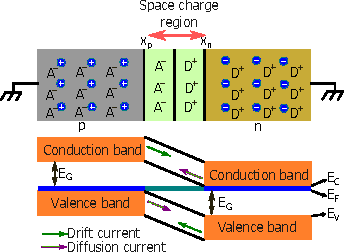
\includegraphics[scale=1]{fig/lec03/band_diagram_pn_junction_big.pdf}
				\caption{Energy band diagram of a p-n junction.}
				\label{fig:pn_junction}
			\end{figure}
		\end{column}
	\end{columns}
\end{frame}

%%%%%%%%%%%%%%%%%%%%%%%%%%%%%%%%%%%%%%%%%%%%%%%%%%%%%%%%%%%%%
%% Key insights in charge movement in p-n junctions %%
%%%%%%%%%%%%%%%%%%%%%%%%%%%%%%%%%%%%%%%%%%%%%%%%%%%%%%%%%%%%%
\begin{frame}
	\frametitle{Key Insights into Charge Movement}
	\begin{columns}
		\begin{column}{0.5\textwidth}
			\begin{itemize}
				\item Initial carrier flow is driven by \textbf{concentration gradients}, not electric forces.
				\item Opposite charges do not attract each other across the junction initially.
				\item The \textbf{electric field is a result of diffusion}, not the cause of it.
				\item The depletion region is characterized by:
				\begin{itemize}
					\item No free carriers
					\item Net space charge from fixed dopants
				\end{itemize}
				\item The system reaches an equilibrium defined by the \textbf{built-in potential} $V_{bi}$.
			\end{itemize}
		\end{column}
		\begin{column}{0.5\textwidth}
			\begin{figure}
				\centering
				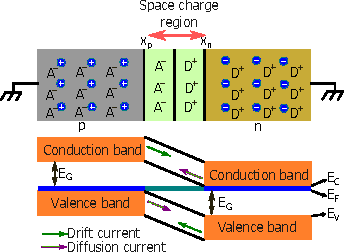
\includegraphics[scale=1]{fig/lec03/band_diagram_pn_junction_big.pdf}
				\caption{Energy band diagram of a p-n junction.}
				\label{fig:pn_junction}
			\end{figure}
		\end{column}
	\end{columns}
\end{frame}


%%%%%%%%%%%%%%%%%%%%%%%%%%%%%%%%%%%%%%%%%%%%%%%%%%%%%%%%%%%%%
%% Electric field intensity in space charge regions %%
%%%%%%%%%%%%%%%%%%%%%%%%%%%%%%%%%%%%%%%%%%%%%%%%%%%%%%%%%%%%%
\begin{frame}{Electric Field Intensity in the scpace charge region}
    \begin{itemize}
        \item The depletion region in a pn junction contains \textbf{uncompensated dopant ions} (donors in n-side, acceptors in p-side).
        \item This fixed charge distribution creates a \textbf{space-charge density} $\rho(x)$, giving rise to an electric field.
        \item According to \textbf{Poisson's equation}:
        \begin{equation}
            \frac{d^2 V}{dx^2} = -\frac{\rho(x)}{\varepsilon}
        \end{equation}
        where $V$ is the electrostatic potential and $\varepsilon$ is the permittivity.

        \item Integrating Poisson's equation yields the electric field:
        \begin{equation}
            \mathcal{E}(x) = \int_{x_p}^x \frac{\rho(x_n)}{\varepsilon} dx
        \end{equation}
        where $x_p$ is the reference point where $\mathcal{E}(x_p) = 0$.
    \end{itemize}
\end{frame}

%%%%%%%%%%%%%%%%%%%%%%%%%%%%%%%%%%%%%%%%%%%%%%%%%%%%%%%%%%%%%
%% Electric field intensity in space charge regions %%
%%%%%%%%%%%%%%%%%%%%%%%%%%%%%%%%%%%%%%%%%%%%%%%%%%%%%%%%%%%%%
\begin{frame}{Electric Field Intensity in the space charge region}
    \begin{itemize}
        \item \textbf{Electric field direction:}
        \begin{itemize}
            \item Points from n-side (positive charge) to p-side (negative charge).
            \item Corresponds to \textbf{negative field intensity} if potential decreases from n to p.
        \end{itemize}
        \item The electric field acts like an \textbf{internal dipole layer}, enabling the concept of \textbf{built-in potential} $V_0$.
		\item \textbf{Equilibrium condition:}
        \item At thermal equilibrium, i.e. the steady-state condition at a given temperature with no external excitations, the
		individual electron and hole currents flowing across the junctions are identically zero. Thus, for each type of
		carrier the drift current due to the electric field must exactly cancel the diffusion current due to the concentration
		gradient.
		\begin{equation}
			j_n = j_p = 0 \Rightarrow j_n + j_p = 0
		\end{equation}
		\item The total current density is given by:
		\begin{equation}
			j = j_n (\text{drift}) + j_p (\text{diffusion}) = q \left( \mu_n n \mathcal{E} + D_n \frac{dn}{dx} - \mu_p p \mathcal{E} - D_p \frac{dp}{dx} \right) = 0
		\end{equation}
    \end{itemize}
\end{frame}

%%%%%%%%%%%%%%%%%%%%%%%%%%%%%%%%%%%%%%%%%%%%%%%%%%%%%%%%%%%%%
% Built-in Voltage: Starting with Einstein Relation and Drift-Diffusion#
%%%%%%%%%%%%%%%%%%%%%%%%%%%%%%%%%%%%%%%%%%%%%%%%%%%%%%%%%%%%%
\begin{frame}{Built-in Voltage: Einstein Relation and Carrier Distribution}
    \begin{itemize}
        \item From the Einstein relation, the drift-diffusion equations become:
        \begin{align}
            j_n &= q \mu_n \left( n \mathcal{E} + \frac{kT}{q} \frac{dn}{dx} \right)  \\
            j_p &= q \mu_p \left( p \mathcal{E} - \frac{kT}{q} \frac{dp}{dx} \right) 
        \end{align}
        \item At equilibrium ($j_p = 0$), using integration of the expression inside the bracket gives:
        \begin{equation}
            p(x) = p(x_p) e^{-\frac{qV(x)}{kT}}
        \end{equation}
        \item With $V(x) = - \int_{x_p}^{x} \mathcal{E}(x') dx'$
        \item Similarly for electrons:
        \begin{equation}
            n(x) = n(x_n) e^{\frac{qV(x)}{kT}} 
        \end{equation}
        \item These distributions are referred to as the \textbf{Boltzmann distribution} under equilibrium.
    \end{itemize}
\end{frame}

%%%%%%%%%%%%%%%%%%%%%%%%%%%%%%%%%%%%%%%%%%%%%%%%%%%%%%%%%%%%%
% Built-in Potential Derivation
%%%%%%%%%%%%%%%%%%%%%%%%%%%%%%%%%%%%%%%%%%%%%%%%%%%%%%%%%%%%%
\begin{frame}{Derivation of Built-in Potential $V_{bi}$}
    \begin{itemize}
        \item Carrier product at any point:
        \begin{equation}
            n \cdot p = n_i^2 
        \end{equation}
        \item Built-in potential is given by:
        \begin{equation}
            V_{bi} = V(x_n) = \frac{kT}{q} \ln\left( \frac{p(x_p)}{p(x_n)} \right) = \frac{kT}{q} \ln\left( \frac{p(x_p) \cdot n(x_n)}{n_i^2} \right) 
        \end{equation}
        \item Assuming complete ionization at boundaries:
        \begin{equation}
            V_{bi} \cong \frac{kT}{q} \ln\left( \frac{N_A(x_p) \cdot N_D(x_n)}{n_i^2} \right) 
        \end{equation}
        \item This shows that $V_{bi}$ depends only on the doping levels and intrinsic carrier concentration.
        \item Important for setting the electrostatic barrier preventing further diffusion across the junction.
    \end{itemize}
\end{frame}

%%%%%%%%%%%%%%%%%%%%%%%%%%%%%%%%%%%%%%%%%%%%%%%%%%%%%%%%%%%%%
% Summary and insights in built-in potential
%%%%%%%%%%%%%%%%%%%%%%%%%%%%%%%%%%%%%%%%%%%%%%%%%%%%%%%%%%%%%
\begin{frame}{Key Insights from Built-in Potential Derivation}
    \begin{itemize}
		\item \textbf{1. Drift-Diffusion Balance at Equilibrium}
		\begin{itemize}
			\item Currents consist of drift + diffusion components.
			\item At equilibrium: $j_n = j_p = 0 \Rightarrow$ drift current = $-$ diffusion current.
		\end{itemize}

        \item \textbf{2. Carrier Densities Follow Boltzmann Distributions}
        \begin{itemize}
            \item $p(x) = p(x_p) e^{-\frac{qV(x)}{kT}},\quad n(x) = n(x_n) e^{\frac{qV(x)}{kT}}$
            \item Potential $V(x)$ governs spatial variation in carrier concentration.
        \end{itemize}

        \item \textbf{3. Mass Action Law Holds:} $n(x) \cdot p(x) = n_i^2$ \textit{everywhere in depletion region}

        \item \textbf{4. Built-in Voltage Expression:}
        \begin{equation}
            V_{bi} = \frac{kT}{q} \ln\left(\frac{N_A(x_p) \cdot N_D(x_n)}{n_i^2}\right)
		\end{equation}
        \begin{itemize}
            \item Depends only on doping densities and intrinsic carrier concentration.
            \item Sets up internal electrostatic barrier to prevent further diffusion.
        \end{itemize}

        \item \textbf{5. Interpretation:}
        \begin{itemize}
            \item \textit{Defines equilibrium energy band bending and barrier height.}
            \item \textit{Logarithmic dependence allows efficient doping control of $V_{bi}$.}
        \end{itemize}
    \end{itemize}
\end{frame}


%%%%%%%%%%%%%%%%%%%%%%%%%%%%%%%%%%%%%%%%%%%%%%%%%%%%%%%%%%%%%
% Biasing of p-n junctions
%%%%%%%%%%%%%%%%%%%%%%%%%%%%%%%%%%%%%%%%%%%%%%%%%%%%%%%%%%%%%
\begin{frame}{Biasing of p-n junctions}
	\textbf{All discussions in the previous slides were based on the assumption of thermal equilibrium and no external fields.} \\
	The behavior of a p-n junction can be controlled by applying an external voltage across the junction. \\
	\textbf{Biasing} refers to the application of an external voltage across a p-n junction to control its operation. The two main types of biasing are:
	\begin{columns}
		\begin{column}{0.5\textwidth}
			\begin{itemize}
				\item \textbf{Forward Bias:} Positive voltage applied to the p-side and negative voltage to the n-side.
			\end{itemize}
			\begin{figure}
				\centering
				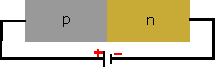
\includegraphics[scale=1]{fig/lec03/pn_forward_bias.pdf}
				\caption{Forward bias of a p-n junction.}
				\label{fig:forward_bias_pn_junction}
			\end{figure}
		\end{column}
		\begin{column}{0.5\textwidth}
			\begin{itemize}
				\item \textbf{Reverse Bias:} Positive voltage applied to the n-side and negative voltage to the p-side.
			\end{itemize}
			\begin{figure}
				\centering
				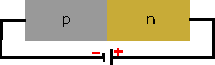
\includegraphics[scale=1]{fig/lec03/pn_reverse_bias.pdf}
				\caption{Reverse bias of a p-n junction.}
				\label{fig:reverse_bias_pn_junction}
			\end{figure}
		\end{column}
	\end{columns}
\end{frame}

%%%%%%%%%%%%%%%%%%%%%%%%%%%%%%%%%%%%%%%%%%%%%%%%%%%%%%%%%%%%%
% Reverse bias of p-n junctions
%%%%%%%%%%%%%%%%%%%%%%%%%%%%%%%%%%%%%%%%%%%%%%%%%%%%%%%%%%%%%

\begin{frame}{Reverse bias in a \textit{p-n} Junction}
    \textbf{Key Concept:} Reverse bias widens the depletion region and blocks majority carrier flow.
    \begin{itemize}
        \item \textbf{Biasing:} Negative terminal to $p$-side, positive to $n$-side (Fig. \ref{fig:reverse_bias_pn_junction}).
        \item \textbf{Effect:} Drives majority carriers (holes in $p$, electrons in $n$) \textit{away} from the junction.
        \item \textbf{Depletion Region:} Widens due to carrier drift, increasing the electric field barrier.
        \item \textbf{Steady State:} Cannot sustain continuous diffusion without replenishment $\Rightarrow$ nominally zero current.
        \item \textbf{Reverse Saturation Current $I_0$:}
        \begin{itemize}
            \item Small current due to minority carriers thermally generated.
            \item $I_0$ increases with temperature, but is \textit{independent} of applied reverse voltage.
        \end{itemize}
        \item \textbf{Physical Insight:} Potential barrier increases by $qV \Rightarrow$ blocks majority carriers, but allows minority carriers to flow.
		\item \textbf{Reverse Bias Breakdown:} If reverse voltage exceeds a critical value, breakdown occurs (Zener or avalanche breakdown).
    \end{itemize}
\end{frame}

%%%%%%%%%%%%%%%%%%%%%%%%%%%%%%%%%%%%%%%%%%%%%%%%%%%%%%%%%%%%%
% Forward bias of p-n junctions
%%%%%%%%%%%%%%%%%%%%%%%%%%%%%%%%%%%%%%%%%%%%%%%%%%%%%%%%%%%%%

\begin{frame}{Forward bias in a \textit{p-n} Junction}
	\begin{columns}
		\begin{column}{0.7\textwidth}
			\textbf{Key Concept:} Forward bias lowers the potential barrier and allows majority carrier injection.
			\begin{itemize}
				\item \textbf{Biasing:} Positive terminal to $p$-side, negative to $n$-side.
				\item \textbf{Effect:} Lowers the junction barrier height by $qV$, aiding carrier diffusion.
				\item \textbf{Depletion Region:} Narrows, reducing the internal electric field.
				\item \textbf{Carrier Movement:}
				\begin{itemize}
					\item Holes from $p$ move into $n$-side $\Rightarrow$ \textit{injected minority current}
					\item Electrons from $n$ move into $p$-side $\Rightarrow$ \textit{minority current in opposite direction}
				\end{itemize}
				\item \textbf{Current Flow:} Resultant current = sum of hole and electron minority currents.
				\item \textbf{Diode Equation:} $I = I_0 \left(e^{qV/kT} - 1\right)$ (derived later)
    	\end{itemize}
	\end{column}
		\begin{column}{0.3\textwidth}
			\begin{figure}
				\centering
				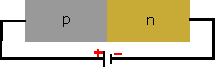
\includegraphics[scale=1]{fig/lec03/pn_forward_bias.pdf}
				\caption{Forward bias of a p-n junction.}
				\label{fig:forward_bias_pn_junction}
			\end{figure}
		\end{column}
	\end{columns}
\end{frame}

%%%%%%%%%%%%%%%%%%%%%%%%%%%%%%%%%%%%%%%%%%%%%%%%%%%%%%%%%%%%%
% Ohmic contacts in of p-n junctions
%%%%%%%%%%%%%%%%%%%%%%%%%%%%%%%%%%%%%%%%%%%%%%%%%%%%%%%%%%%%%

\begin{frame}{\textbf{Ohmic Contacts in \textit{p-n} Junctions}}
    \textbf{Definition:} \textit{Ohmic contacts} are special metal-semiconductor interfaces engineered to allow current to flow freely in both directions, without rectification behavior.

    \vspace{1em}
    \textbf{Key Assumptions:}
    \begin{itemize}
        \item In practical \textit{p-n} diodes, external bias is applied via metal contacts to both the $p$ and $n$ regions.
        \item These contacts create metal-semiconductor junctions — which, in general, could have their own contact potential.
        \item \textbf{Ohmic contacts} are designed to ensure:
        \begin{itemize}
            \item Contact potential remains \textbf{constant}, irrespective of current direction or magnitude.
            \item There is \textbf{no barrier to carrier flow} at the metal-semiconductor interface.
        \end{itemize}
    \end{itemize}
\end{frame}

\begin{frame}{\textbf{Ohmic Contacts in \textit{p-n} Junctions cont..}}
\textbf{Physical Insight:}
\textbf{Justification of Bias Assumption:}
\begin{itemize}
	\item Because the ohmic contacts are nonrectifying and the voltage drop across the bulk crystal is negligible,
	\item $\Rightarrow$ \textbf{Entire external bias appears across the \textit{p-n} junction barrier.}
	\item This simplifies analysis: bias voltage directly modifies the potential barrier height.
\end{itemize}
\textbf{Conclusion:}
\begin{itemize}
	\item Ohmic contacts are \textbf{essential} for accurate modeling of diode behavior under applied bias.
	\item They ensure that changes in applied voltage affect only the junction, not the metal-semiconductor interfaces.
\end{itemize}
\end{frame}


\begin{frame}{\textbf{Short-Circuited and Open-Circuited \textit{p-n} Junction}}
    \textbf{Physical Insight:} The behavior of a \textit{p-n} junction under short-circuit ($V = 0$) or open-circuit conditions ($I = 0$) reveals fundamental principles of equilibrium electrostatics and energy conservation.

    \vspace{0.7em}
    \textbf{Key Points:}
    \begin{itemize}
        \item When $V = 0$ is applied across the \textit{p-n} diode (Fig. \ref{fig:forward_bias_pn_junction} or Fig. \ref{fig:reverse_bias_pn_junction}), the junction is \textbf{short-circuited}.
        \item Under thermal equilibrium, this implies:
        \begin{itemize}
            \item Net current $I = 0$
            \item Junction potential $V_0$ remains unchanged.
        \end{itemize}

        \item \textbf{Energy conservation argument:}
        \begin{itemize}
            \item If current $I \neq 0$, metal wire heats up.
            \item No external energy source exists, so energy must come from \textit{p-n} bar $\Rightarrow$ thermal cooling of bar.
            \item \textbf{Contradiction:} Can't have metal heating and bar cooling simultaneously in equilibrium.
            \item \textbf{Conclusion:} $I = 0$
        \end{itemize}
	\end{itemize}
\end{frame}

\begin{frame}{\textbf{Short-Circuited and Open-Circuited \textit{p-n} Junction}}
	\begin{itemize}
	\item \textbf{Voltage Loop Consistency:}
	\begin{itemize}
		\item Total voltage drop across closed loop must be zero.
		\item $V_0$ is exactly compensated by contact potentials at ohmic contacts.
		\item Even if wire is cut, voltage drop remains zero.
	\end{itemize}

	\item \textbf{Implication:} $V_0$ cannot be measured directly by a voltmeter.
	\end{itemize}

	\vspace{0.7em}
	\textbf{Conclusion:} \textit{Built-in potential $V_0$ exists, but is internally balanced by metal-semiconductor junctions; it is not externally measurable.}
\end{frame}


\begin{frame}{The current components in a \textit{p-n} Junction}
\begin{columns}
		\begin{column}{0.225\textwidth}
	\textbf{Key Idea: Minority carrier injection under forward bias}
	\begin{itemize}
		\item When a forward voltage $V$ is applied:
		\begin{itemize}
			\item Holes are injected from $p$ to $n$ region.
			\item Electrons are injected from $n$ to $p$ region.
		\end{itemize}
	\end{itemize}
\end{column}
\begin{column}{0.775\textwidth}
	\begin{figure}
		\centering
		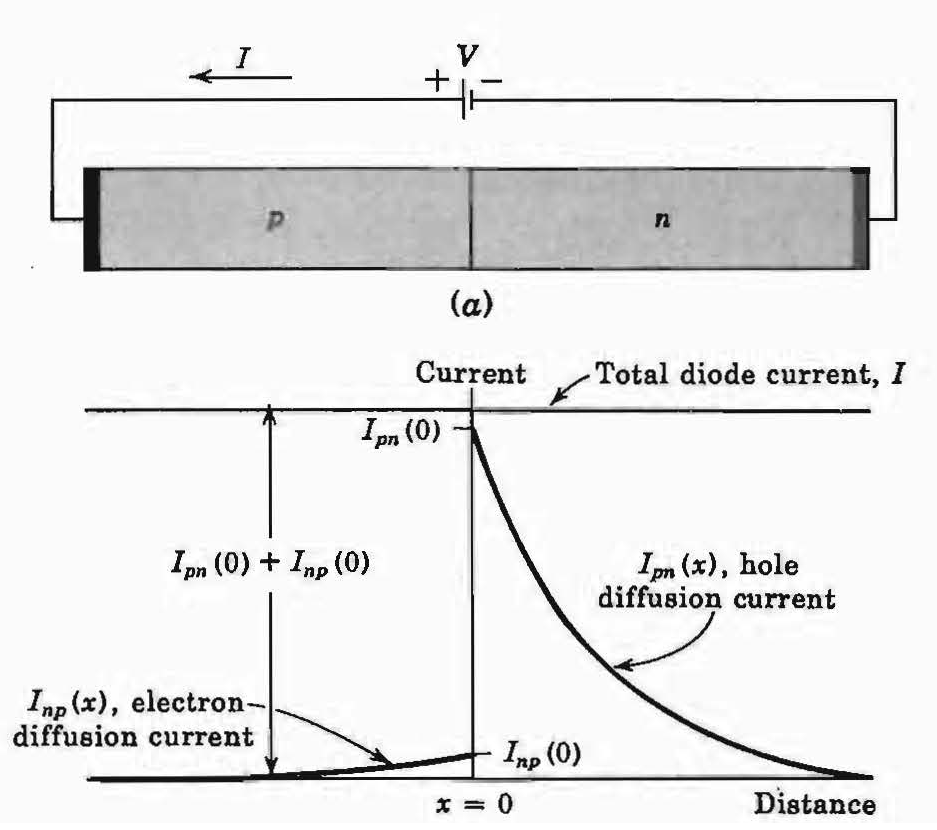
\includegraphics[scale=0.325]{fig/lec03/current_component_in_pn_junction.png}
		\caption{The hole- and electron-current diffusion components vs. distance in a p-n junction diode; adapted from Millman, J., \& Halkias, C. C. Integrated Electronics: Analog and Digital Circuits and Systems.}
		\label{fig:plot_of_pn_junction_current}
	\end{figure}
\end{column}
\end{columns}
\end{frame}

\begin{frame}{Minority Currents in a \textit{p-n} Junction}
	\begin{itemize}
\item Minority carrier current in $n$-type region:
\begin{equation} \label{eq:minority_current_n_region}
	I_{pn}(0) = \frac{AqD_p}{L_p} \left[ p_n(0) - p_{n0} \right]
\end{equation}
where:
\begin{itemize}
	\item $D_p$ = hole diffusion coefficient
	\item $L_p$ = hole diffusion length
	\item $p_n(0)$ = hole concentration at $x = 0$
	\item $p_{n0}$ = equilibrium minority hole concentration
\end{itemize}
\item From law of the junction:
\begin{equation} \label{eq:law_of_junction}
	p_n(0) = p_{n0} e^{\frac{V}{V_T}} \quad
\end{equation}
\end{itemize}

\end{frame}

\begin{frame}{Minority Currents in a \textit{p-n} Junction}
	\begin{itemize}
	\item Substituting Eq. \ref{eq:law_of_junction} into Eq. \ref{eq:minority_current_n_region} gives:
	\begin{equation}
		I_{pn}(0) = \frac{AqD_p p_{n0}}{L_p} \left( e^{\frac{V}{V_T}} - 1 \right)
	\end{equation}

	\item Similarly for electron diffusion:
	\begin{equation}
		I_{np}(0) = \frac{AqD_n n_{p0}}{L_n} \left( e^{\frac{V}{V_T}} - 1 \right)
	\end{equation}

	\item \textbf{Total diode current:}
	\begin{equation}
		I = I_0 \left( e^{\frac{V}{V_T}} - 1 \right)
	\end{equation}
	where:
	\begin{equation*}
		I_0 = \frac{Aq}{L_p} D_p p_{n0} + \frac{Aq}{L_n} D_n n_{p0}
	\end{equation*}
	\item $I_0$ is the reverse saturation current.
	\end{itemize}
\end{frame}	

	
\begin{frame}{Majority Carrier Currents and Total Current Distribution}
	\begin{columns}
		\begin{column}{0.225\textwidth}
	\textbf{Current Continuity and Carrier Profile:}
	\begin{itemize}
		\item Under forward bias, minority carrier current varies with $x$:
		\begin{itemize}
			\item $I_{pn}(x)$ (hole current) decreases exponentially in $n$-region.
			\item $I_{np}(x)$ (electron current) decreases exponentially in $p$-region.
		\end{itemize}
	\end{itemize}
\end{column}
		\begin{column}{0.775\textwidth}
	\begin{figure}	
		\centering
		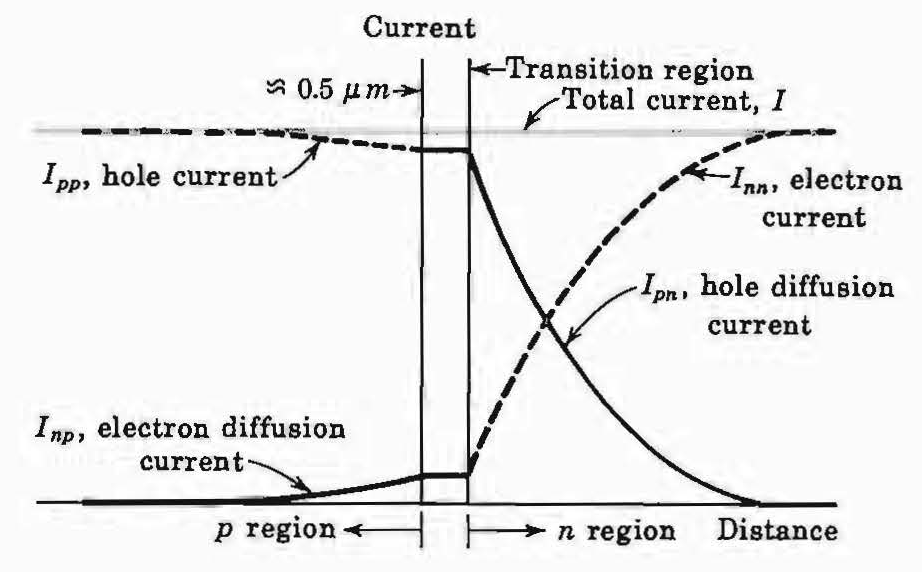
\includegraphics[scale=0.325]{fig/lec03/majority_and_minority_vs_distance.png}
		\caption{The minority (solid) end the majority (dashed) currents vs. distance
		in a p-n diode. lt is assumed that no recombination takes place in the very	narrow depletion region.; adapted from Millman, J., \& Halkias, C. C. Integrated Electronics: Analog and Digital Circuits and Systems.}
		\label{fig:minority_and_majority_current}
	\end{figure}
	\end{column}
	\end{columns}
\end{frame}


\begin{frame}{Majority Carrier Currents and Total Current Distribution}
\begin{itemize}
\item \textbf{To maintain constant total current $I$ across the junction:}
\begin{equation}
	I_{nn}(x) = I - I_{pn}(x), \quad I_{pp}(x) = I - I_{np}(x)
\end{equation}
where:
\begin{itemize}
	\item $I_{nn}(x)$ is majority (electron) current in $n$ region
	\item $I_{pp}(x)$ is majority (hole) current in $p$ region
\end{itemize}

\item \textbf{Total current is bipolar in nature}:
\begin{itemize}
	\item Composed of hole and electron contributions
	\item Varies spatially due to recombination
\end{itemize}
\item Transition region assumed to have negligible recombination width (valid for Si)
\end{itemize}
\end{frame}

	\begin{frame}{Volt-Ampere Characteristic of a \textit{p-n} Diode}
	\textbf{General Current Equation:}
	\begin{equation}
		I = I_0 \left( e^{\frac{V}{\eta V_T}} - 1 \right)
	\end{equation}
	\begin{itemize}
		\item $I_0$ = reverse saturation current
		\item $V$ = applied voltage
		\item $V_T = \frac{kT}{q}$ = thermal voltage ($\approx 26$ mV at 300 K)
		\item $\eta$ = ideality factor ($\approx 1$ for Ge, $\approx 2$ for Si)
	\end{itemize}
	
	\textbf{Interpretation:}
	\begin{itemize}
		\item For $V \gg V_T$: exponential current rise (forward bias)
		\item For $V < 0$: $I \approx -I_0$ (reverse saturation current)
	\end{itemize}

\end{frame}


\begin{frame}{\textbf{Reverse Saturation Current and Breakdown Behavior}}
	\begin{columns}
		\begin{column}{0.25\textwidth}
    	\begin{itemize}
        \item \textbf{Reverse Saturation Current} ($I_0$):
        \begin{itemize}
            \item For reverse bias $V < 0$, diode current saturates to $I = -I_0$.
            \item $I_0$ is weakly dependent on reverse voltage.
            \item Caused by thermally generated minority carriers.
            \item Germanium diodes have $I_0$ \textasciitilde{}1000x larger than silicon.
        \end{itemize}
	\end{itemize}
		\end{column}
		\begin{column}{0.75\textwidth}
	\begin{figure}
		\centering
		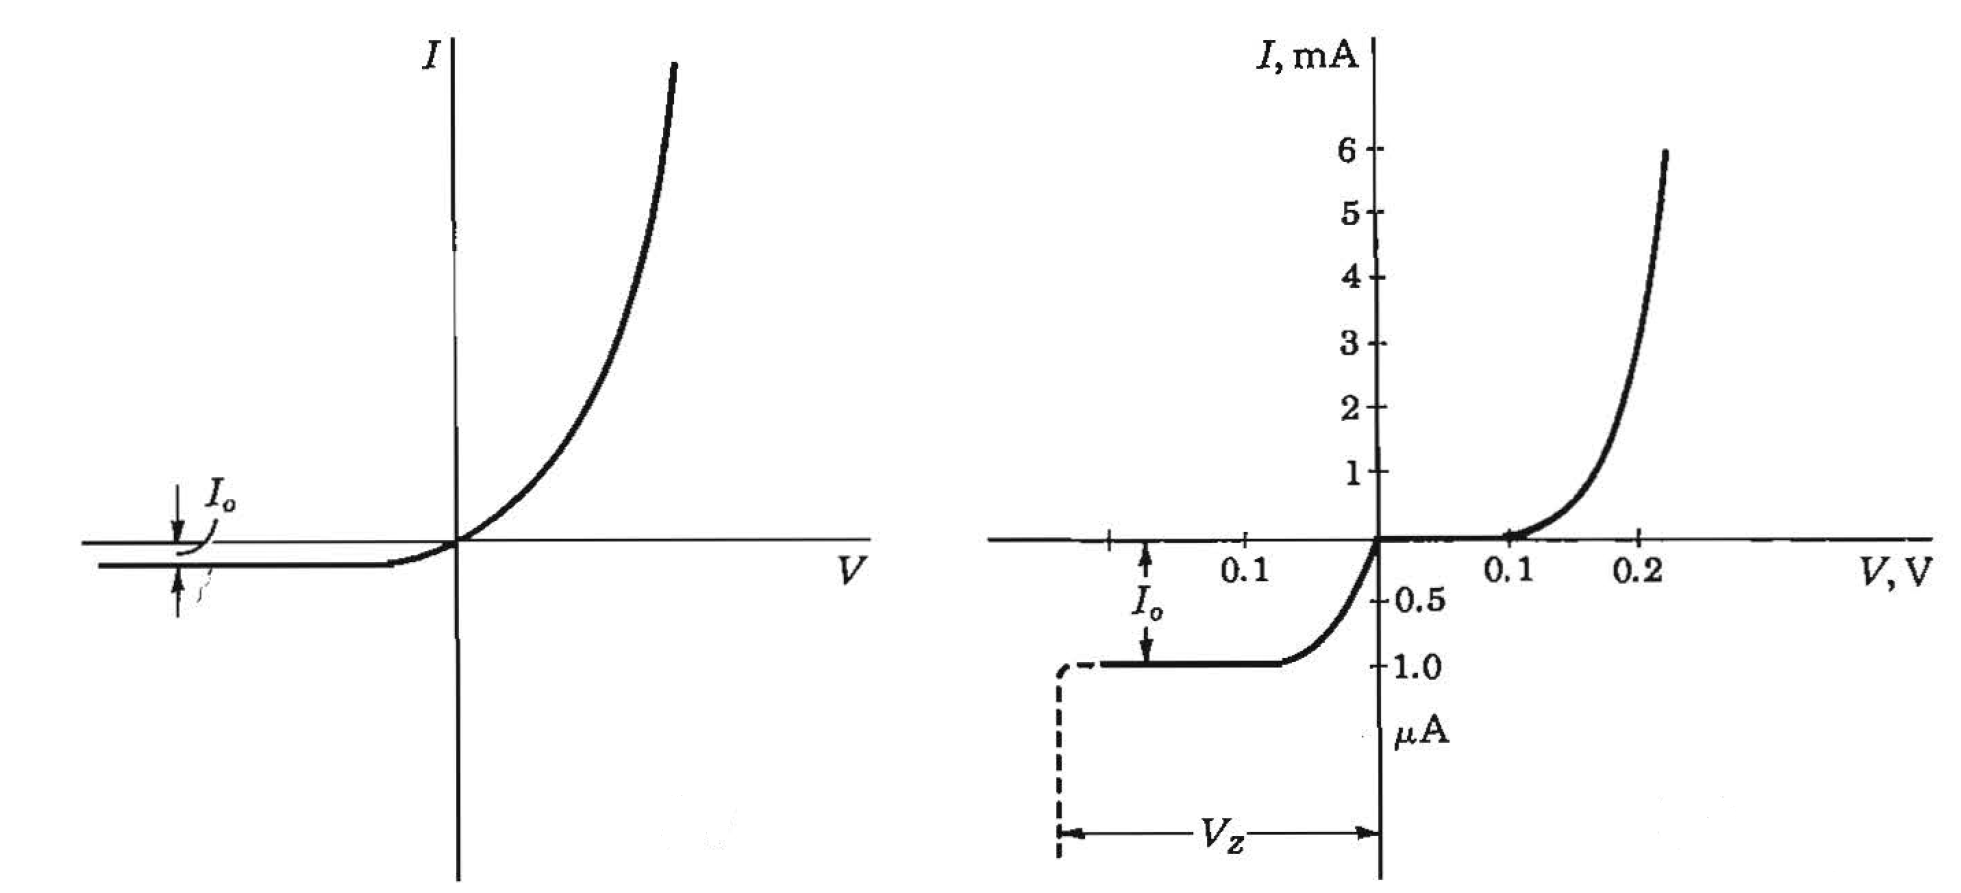
\includegraphics[scale=0.25]{fig/lec03/VI_characteristics.png}
		\caption{The volt-ampere characteristic of an ideal p-n diode and the volt-ampere characteristic for a germanium; adapted from Millman, J., \& Halkias, C. C. Integrated Electronics: Analog and Digital Circuits and Systems.}
		\label{fig:diode_characteristics}
	\end{figure}
	\end{column}
	\end{columns}
\end{frame}

\begin{frame}{\textbf{Reverse Saturation Current and Breakdown Behavior}}
	\begin{columns}
		\begin{column}{0.225\textwidth}
\begin{itemize}
	\item \textbf{Breakdown Region:}
	\begin{itemize}
		\item At a reverse voltage $V_Z$, breakdown occurs $\Rightarrow$ sudden increase in $I$.
		\item Caused by impact ionization or Zener effect.
		\item Fig. 3-6b illustrates abrupt transition at $V_Z$.
	\end{itemize}
\end{itemize}
\end{column}
\begin{column}{0.775\textwidth}
	\begin{figure}
		\centering
		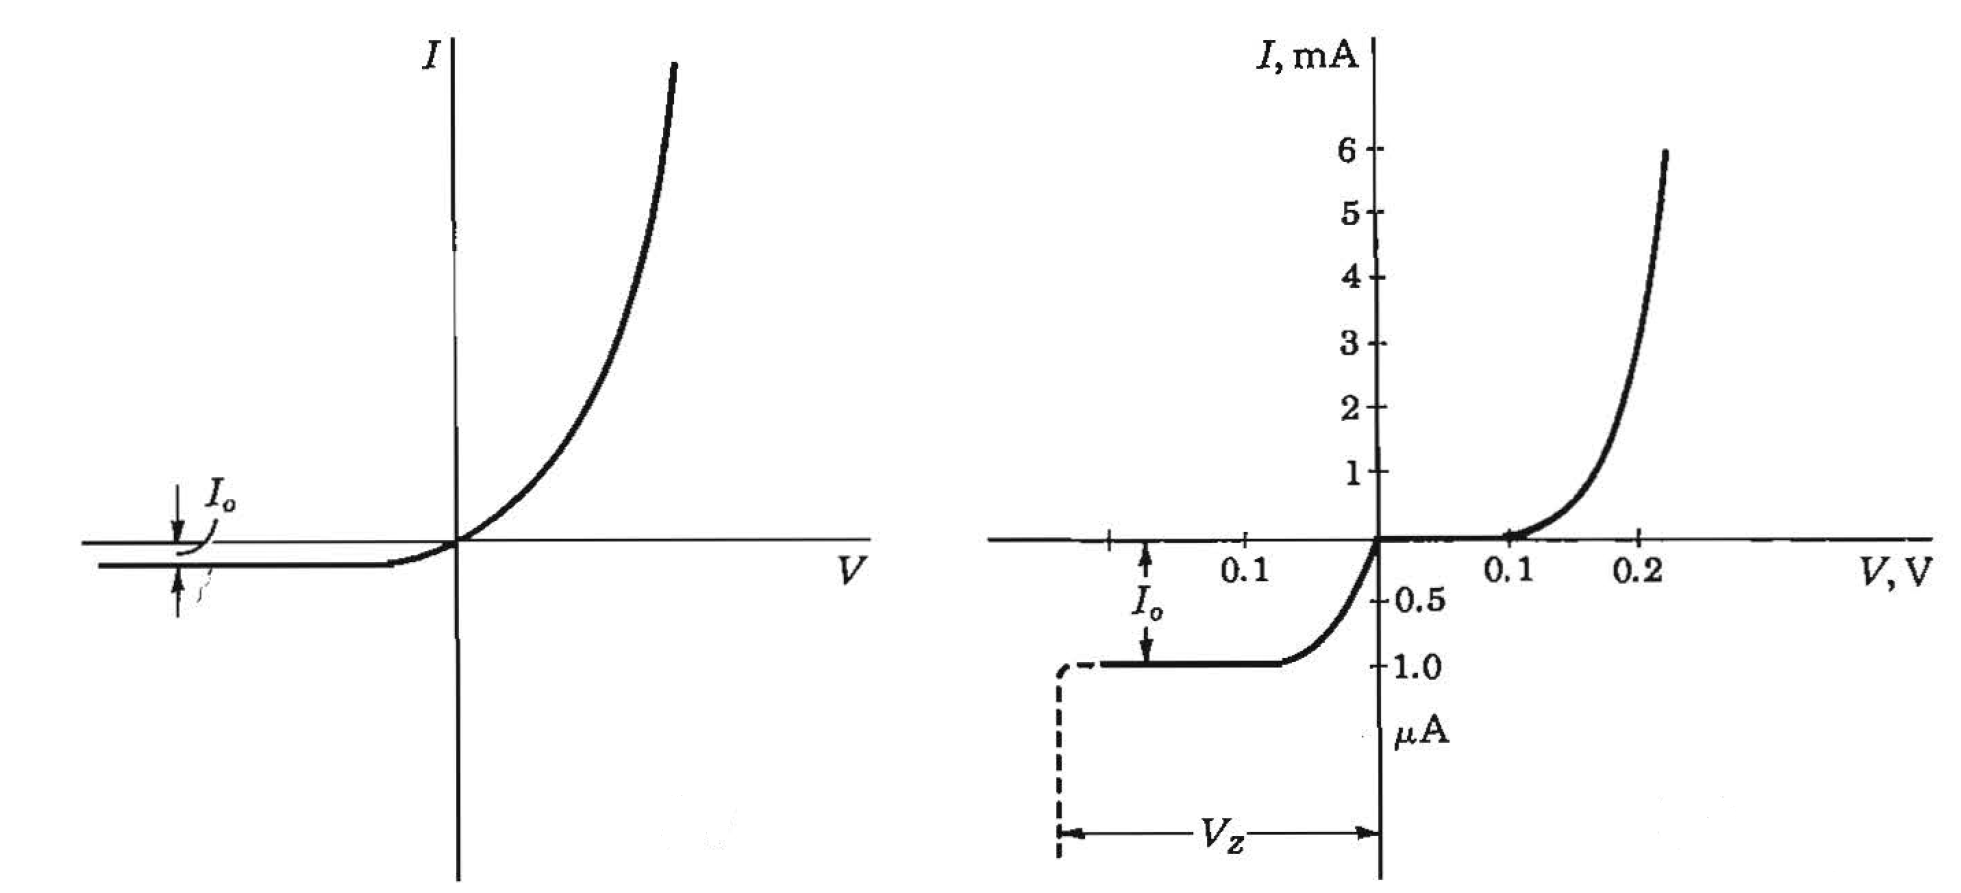
\includegraphics[scale=0.25]{fig/lec03/VI_characteristics.png}
		\caption{The volt-ampere characteristic of an ideal p-n diode and the volt-ampere characteristic for a germanium; adapted from Millman, J., \& Halkias, C. C. Integrated Electronics: Analog and Digital Circuits and Systems.}
		\label{fig:diode_characteristics}
	\end{figure}
	\end{column}
	\end{columns}
\end{frame}



\begin{frame}{\textbf{Cut-in Voltage and Material Comparison}}
	\begin{columns}
		\begin{column}{0.35\textwidth}
    \begin{itemize}
        \item \textbf{Cut-in / Threshold Voltage ($V_\gamma$):}
        \begin{itemize}
            \item Minimum forward bias for noticeable current.
            \item Typically $V_\gamma \approx 0.2$ V (Ge), $\approx 0.6$ V (Si).
            \item Beyond $V_\gamma$, current increases rapidly $\Rightarrow$ exponential growth.
        \end{itemize}
	\end{itemize}
\end{column}
\begin{column}{0.65\textwidth}
	\begin{figure}
		\centering
		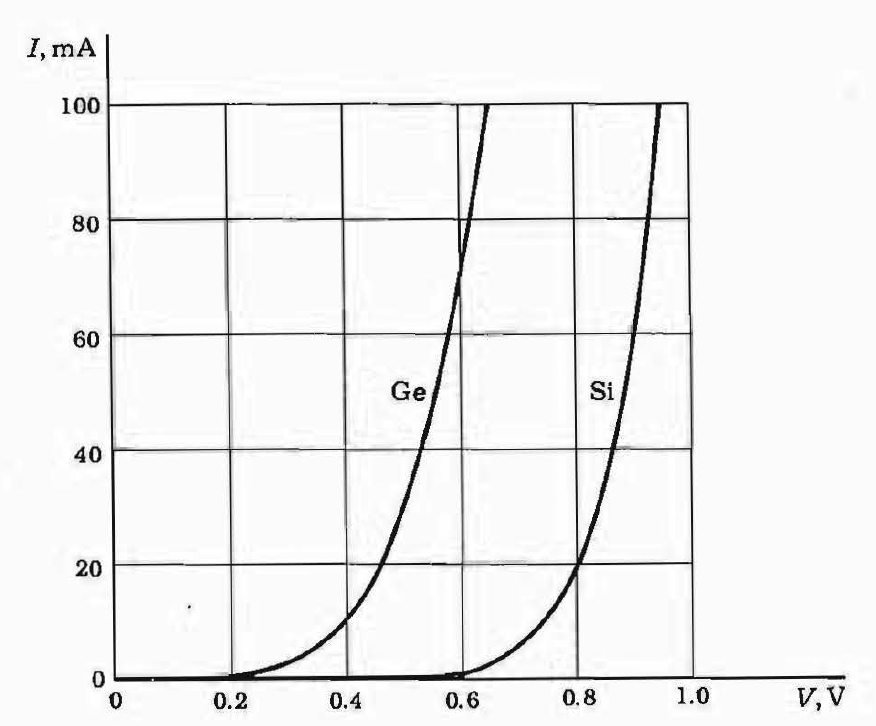
\includegraphics[scale=0.25]{fig/lec03/VI_character_Si_Ge.png}
		\caption{Forward VI characteristics of Si and Ge; adapted from Millman, J., \& Halkias, C. C. Integrated Electronics: Analog and Digital Circuits and Systems.}
		\label{fig:Si_Ge_diode_characteristics}
	\end{figure}
	\end{column}
	\end{columns}
\end{frame}


\begin{frame}{\textbf{Cut-in Voltage and Material Comparison}}
	\begin{columns}
		\begin{column}{0.35\textwidth}
    \begin{itemize}
        \item \textbf{Material Differences:}
        \begin{itemize}
            \item Ge diodes: Lower $V_\gamma$, larger $I_0$, steeper characteristics.
            \item Si diodes: Higher $V_\gamma$, lower $I_0$, more thermal stability.
        \end{itemize}
        \item \textbf{Fig. \ref{fig:Si_Ge_diode_characteristics}:} Comparative $I$-$V$ of 1N270 (Ge) vs 1N3605 (Si).
    \end{itemize}
\end{column}
\begin{column}{0.65\textwidth}
	\begin{figure}
		\centering
		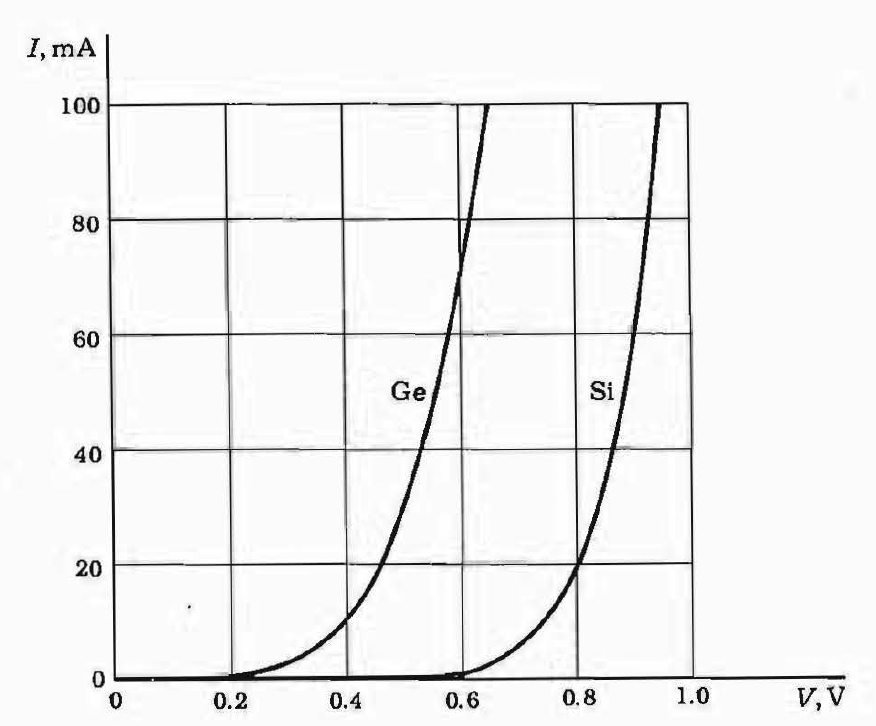
\includegraphics[scale=0.25]{fig/lec03/VI_character_Si_Ge.png}
		\caption{Forward VI characteristics of Si and Ge; adapted from Millman, J., \& Halkias, C. C. Integrated Electronics: Analog and Digital Circuits and Systems.}
		\label{fig:Si_Ge_diode_characteristics}
	\end{figure}
	\end{column}
	\end{columns}
\end{frame}

\begin{frame}{\textbf{Temperature Dependence and $I_0$}}
	\begin{columns}
		\begin{column}{0.5\textwidth}
    \begin{itemize}
        \item $I_0$ increases with temperature:
        \begin{itemize}
            \item $I_0(T) = I_{01} \times 2^{(T - T_1)/10}$
            \item $\Rightarrow$ doubles for every $10^\circ$C rise.
        \end{itemize}
        \item \textbf{Thermal Impact:}
        \begin{itemize}
            \item $V_T = \frac{T}{11600}$ V
            \item At room temp ($300K$), $V_T = 26$ mV
            \item $\left|\frac{dV}{dT}\right| \approx 2.5$ mV/$^\circ$C
        \end{itemize}
        \item Fig. \ref{fig:temp_Si_diode_characteristics} shows $I$-$V$ shifts with temperature: Higher $T \Rightarrow$ lower $V_\gamma$
    \end{itemize}
\end{column}
\begin{column}{0.5\textwidth}
	\begin{figure}
		\centering
		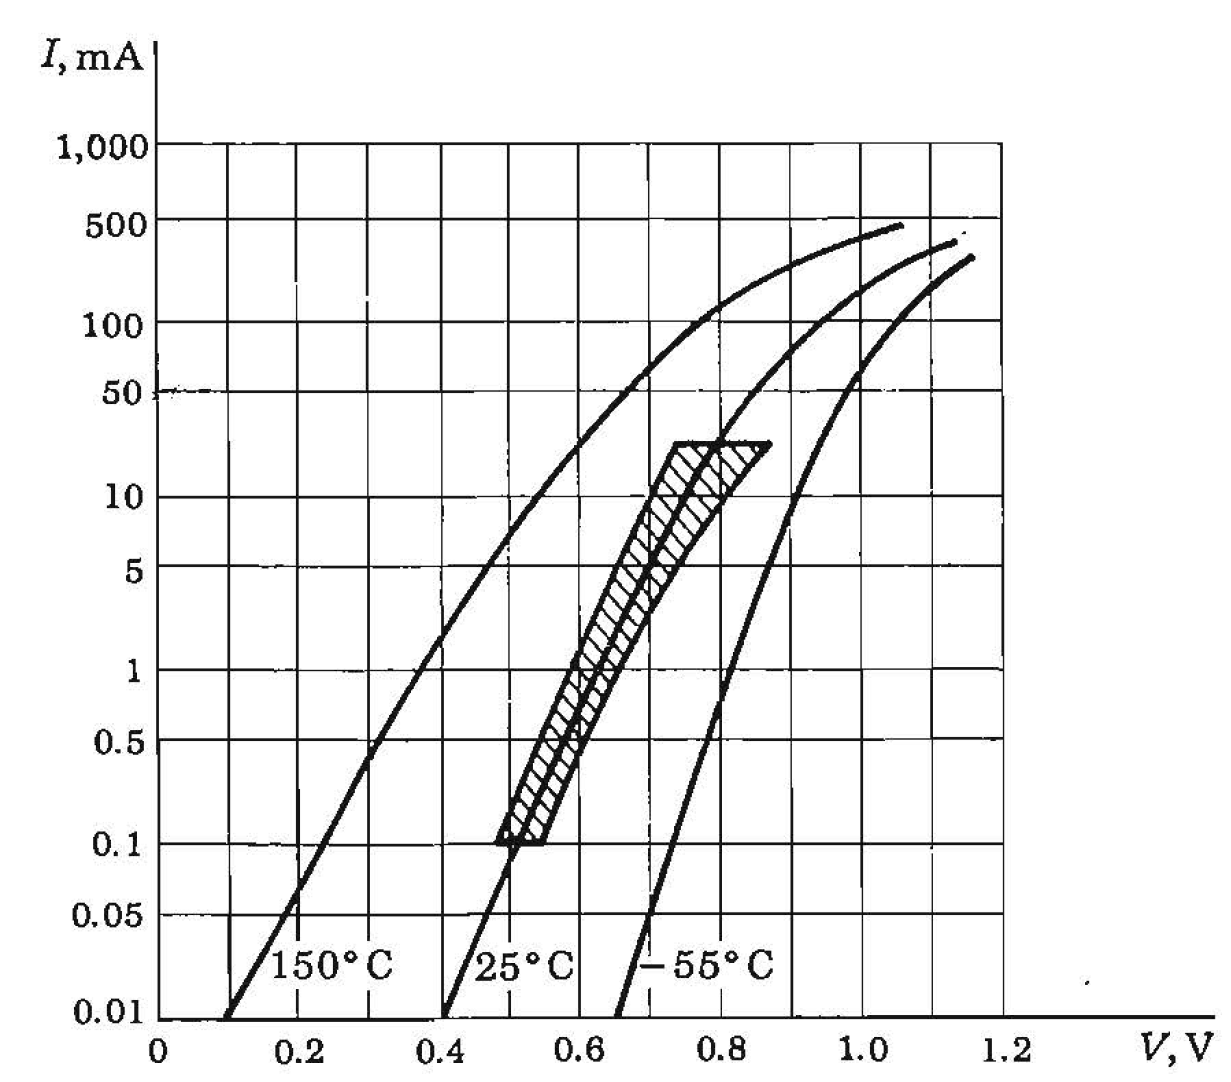
\includegraphics[scale=0.225]{fig/lec03/Temp_dependance.png}
		\caption{VI characteristics at three different	temperatures for a silicon
		diode; adapted from Millman, J., \& Halkias, C. C. Integrated Electronics: Analog and Digital Circuits and Systems.}
		\label{fig:temp_Si_diode_characteristics}
	\end{figure}
	\end{column}
	\end{columns}
\end{frame}

\begin{frame}{\textbf{Diode Resistance and Piecewise Linear Model}}
    \begin{itemize}
        \item \textbf{Static Resistance:} $R = V/I$ \textemdash{} not reliable.
        \item \textbf{Dynamic Resistance:}
        \begin{equation*}
            r = \frac{\eta V_T}{I}
        \end{equation*}
        \item \textbf{Dynamic Conductance:}
        \begin{equation*}
            g = \frac{1}{r} = \frac{I + I_0}{\eta V_T}
        \end{equation*}
        \item \textbf{Piecewise Linear Model:}
        \begin{itemize}
            \item Diode \textasciitilde{} open circuit if $V < V_\gamma$
            \item For $V > V_\gamma$: $r = dV/dI$ constant $\Rightarrow$ $R_f$
            \item Fig. \ref{fig:diode_characteristics}: Diode modeled with $V_\gamma$ and slope $1/R_f$
        \end{itemize}
    \end{itemize}
\end{frame}

\begin{frame}{\textbf{Transition Capacitance ($C_T$)}}
    \begin{itemize}
        \item Under reverse bias, depletion region widens $\Rightarrow$ increase in uncovered charge.
        \item Defined as:
        \begin{equation*}
            C_T = \left| \frac{dQ}{dV} \right|
        \end{equation*}
        \item \textbf{Corresponding Current:}
        \begin{equation*}
            i = C_T \frac{dV}{dt}
        \end{equation*}
        \item $C_T$ is voltage dependent, unlike a linear capacitor.
        \item Important in high-frequency and switching circuits.
    \end{itemize}
\end{frame}


\begin{frame}{\textbf{Diffusion Capacitance: Concept and Static Derivation}}
	\begin{itemize}
		\item \textbf{When forward biased:}
		\begin{itemize}
			\item Excess charge is injected into the neutral region.
			\item Results in large capacitance — called \textbf{diffusion capacitance}, $C_D$.
		\end{itemize}
		
		\item \textbf{Definition:}
		\[
		C_D = \left. \frac{dQ}{dV} \right|_{\text{forward bias}} \quad \text{(rate of change of stored charge w.r.t. voltage)}
		\]
	
		\item \textbf{Using:}
		\begin{align*}
			C_D &= \tau \frac{dI}{dV} = \tau g = \frac{\tau}{r} \tag{3-27} \\
			\Rightarrow C_D &= \frac{\tau I}{\eta V_T} \tag{3-28}
		\end{align*}
		\item Here:
		\begin{itemize}
			\item $\tau$ = carrier lifetime (mean time minority carrier remains mobile)
			\item $I$ = diode current (assumed due to holes)
			\item $\eta$ = ideality factor ($\approx 1$ for Ge, $\approx 2$ for Si)
			\item $V_T = \frac{kT}{q}$ = thermal voltage
		\end{itemize}
	\end{itemize}
	\end{frame}

	\begin{frame}{\textbf{Dynamic Diffusion Capacitance: Arbitrary and Sinusoidal Inputs}}
		\begin{itemize}
			\item \textbf{Implication:} $C_D \propto I$ (linearly dependent on current)
	
			\item \textbf{Time constant:}
			\begin{equation}
			r C_D = \tau \tag{3-29}
			\end{equation}
			where $r = \eta V_T / I$ is the diode dynamic resistance.
			\item \textbf{In general:}
			\begin{equation}
			i = \frac{dQ'}{dt} = C_D' \frac{dV}{dt} \tag{3-30}
			\end{equation}
			\item $C_D' < C_D$ when input varies rapidly.
		
			\item \textbf{Dynamic capacitance:}
			\begin{equation}
			i \neq \frac{dQ}{dt}, \quad i \neq C_D \frac{dV}{dt} \tag{3-31}
			\end{equation}
			since $Q'$ accounts only for instantaneously injected charge, not steady-state.
		\end{itemize}
	\end{frame}	


	\begin{frame}{\textbf{Dynamic Diffusion Capacitance: Arbitrary and Sinusoidal Inputs}}
		\begin{itemize}			
				\item \textbf{For sinusoidal voltage input:}
				\begin{itemize}
					\item Low frequency ($\omega \tau \ll 1$):
					\begin{equation}
					C_D' = \frac{1}{2} \tau g \tag{3-32}
					\end{equation}
					\item High frequency ($\omega \tau \gg 1$):
					\begin{equation}
					C_D' = \left( \frac{\tau}{2\omega} \right)^{1/2} g \tag{3-33}
					\end{equation}
					\item $g = dI/dV = \text{diode conductance}$
				\end{itemize}
			
				\item \textbf{Key Insight:}
				\begin{itemize}
					\item $C_D'$ is frequency-dependent.
					\item Decreases as frequency increases.
					\item Must solve continuity equations to fully describe $C_D'(x,t)$ under general conditions.
				\end{itemize}
		\end{itemize}
	\end{frame}	 % pn junctions and diodes
\section{Introduction to Power Semiconductor Devices}
\title[Introduction to power semiconductor devices]{Introduction to power semiconductor devices}  

\subsection{Power diodes}

\begin{frame}[plain]
    \titlepage
\end{frame}

\begin{frame}{\textbf{Normal vs Power Semiconductor Devices: Key Differences}}
    \textbf{1. Physical Design:}
    \begin{itemize}
        \item \textbf{Normal Devices:} Small device areas, thin active regions for fast operation.
        \item \textbf{Power Devices:} Large device areas, thick drift regions to support high voltages; trade-off between speed and ruggedness.
    \end{itemize}

    \textbf{2. Key Parameters:}
    \begin{itemize}
        \item \textbf{Normal Devices:} Optimize \textit{speed}, \textit{gain}, \textit{integration density}.
        \item \textbf{Power Devices:} Optimize \textit{breakdown voltage}, \textit{on-resistance}, \textit{thermal management}.
    \end{itemize}

    \textbf{3. Material and Fabrication:}
    \begin{itemize}
        \item \textbf{Normal Devices:} Primarily Silicon (Si).
        \item \textbf{Power Devices:} Silicon (Si), but also wide bandgap materials like Silicon Carbide (SiC) and Gallium Nitride (GaN) for superior performance.
    \end{itemize}

    \textbf{4. Examples:}
    \begin{itemize}
        \item \textbf{Normal Devices:} CMOS transistors, Bipolar Junction Transistors (BJTs).
        \item \textbf{Power Devices:} MOSFETs, IGBTs, Diodes (Schottky, PIN), SiC MOSFETs, GaN HEMTs.
    \end{itemize}

    \vspace{0.3cm}
    \textbf{Summary:} \\
    \textit{While normal semiconductors are optimized for information processing, power semiconductors are engineered for robust control of large electrical energy flows.}
\end{frame}


%%%%%%%%%%%%%%%%%%%%%%%%%%%%%%%%%%%%%%%%%%%%%%%%%%%%%%%%%%%%%
%% Conceptual idea of power semiconductor devices physics %%
%%%%%%%%%%%%%%%%%%%%%%%%%%%%%%%%%%%%%%%%%%%%%%%%%%%%%%%%%%%%%
\begin{frame}
	\frametitle{Conceptual idea of a power semiconductor devices physics}
    \textbf{1. Charge Carriers:} 
    \begin{itemize}
        \item Power devices rely on the transport of \textbf{electrons} and \textbf{holes}.
        \item Key mechanisms: \textbf{drift} (due to electric fields) and \textbf{diffusion} (due to concentration gradients).
    \end{itemize}

    \textbf{2. Energy Bands and Junctions:}
    \begin{itemize}
        \item Junctions (e.g., p-n junctions, Schottky barriers) control carrier flow.
        \item Band bending creates potential barriers essential for device blocking and switching behavior.
    \end{itemize}

    \textbf{3. Electric Field Distribution:}
    \begin{itemize}
        \item High electric fields are engineered to manage breakdown and switching.
        \item \textbf{Critical electric field} (\( E_{crit} \)) defines breakdown limits.
    \end{itemize}
\end{frame}


\begin{frame}
	\frametitle{Conceptual idea of a power semiconductor devices physics cond.. }
\textbf{4. Key Physical Processes:}
\begin{itemize}
    \item \textbf{Avalanche Multiplication:} Carrier generation at high fields.
    \item \textbf{Recombination-Generation:} Determines carrier lifetimes.
    \item \textbf{Tunneling:} Important in very high field conditions (Zener breakdown).
\end{itemize}

\textbf{5. Device Performance Metrics:}
\begin{itemize}
    \item \textbf{Blocking Voltage:} Ability to withstand high reverse voltages.
    \item \textbf{On-State Resistance:} Determines conduction losses.
    \item \textbf{Switching Speed:} Influenced by carrier lifetimes and device capacitances.
\end{itemize}

\textbf{Summary:} \\
\textit{Power semiconductor devices are engineered by carefully controlling material properties, doping profiles, junction designs, and carrier dynamics to optimize switching behavior, conduction losses, and voltage handling capabilities.}
\end{frame}

\begin{frame}
	\frametitle{Classification of types of power semiconductor devices}
    \textbf{Based on number of terminals:}
    \begin{columns}
        \column{0.35\textwidth}
        \begin{itemize}
            \item \textbf{Two-terminal devices:}
            \begin{itemize}
                \item Diodes (e.g., Schottky, Zener, and standard rectifier diodes).
            \end{itemize}
            \item \textbf{Three-terminal devices:}
            \begin{itemize}
                \item Insulated Gate Bipolar Transistor (IGBT).
                \item Thyristors (SCRs).
            \end{itemize}
            \item \textbf{Four-terminal devices:}
            \begin{itemize}
                \item IGBT with Kelvin connection.
                \item Cascode structures (e.g., GaN HEMT with a low-voltage MOSFET).
            \end{itemize}
        \end{itemize}

        \column{0.65\textwidth}
        \begin{figure}
            \centering
            \label{fig:Classification_based_on_number_of_terminals}
            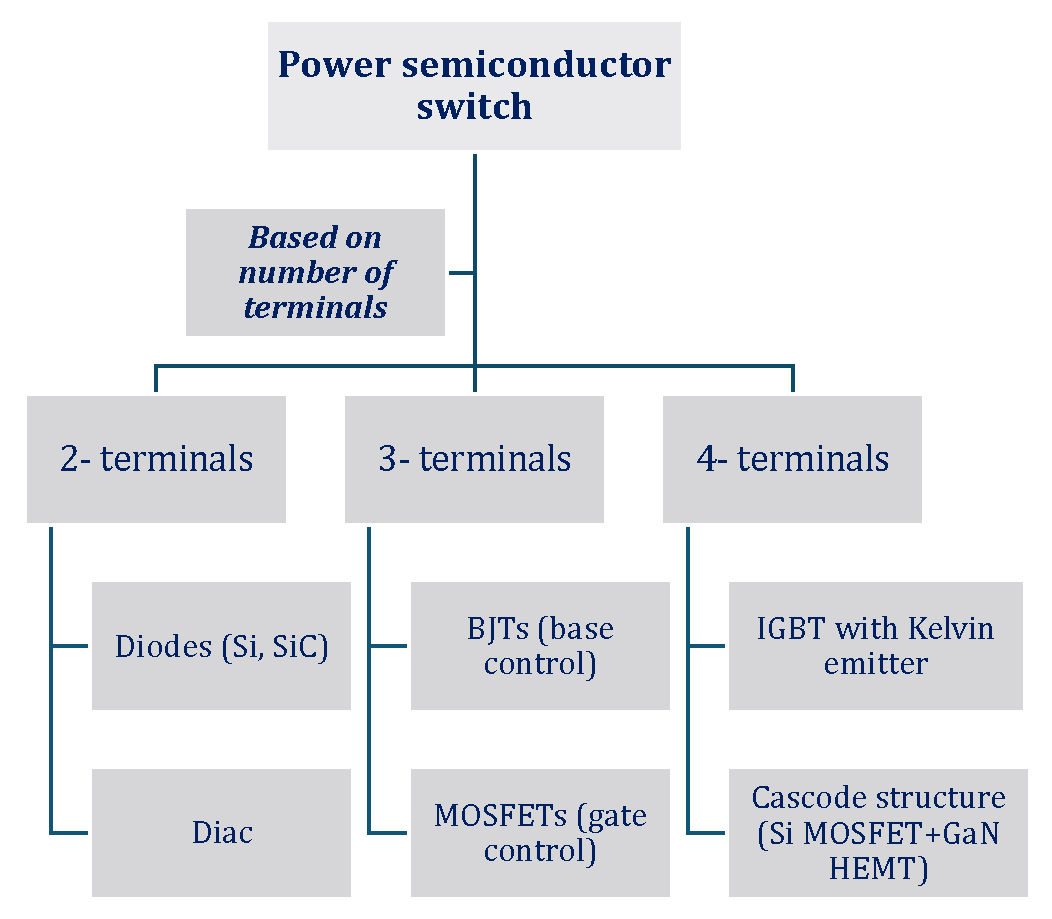
\includegraphics[scale=0.35]{fig/lec04/classification_of_device_1.eps}
            \caption{Classification of power semiconductor devices based on number of terminals.}
        \end{figure}
    \end{columns}
\end{frame}


\begin{frame}
	\frametitle{Classification of types of power semiconductor devices}
    \textbf{Based on number of layser/junctions:}
    \begin{columns}
        \column{0.35\textwidth}
        \begin{itemize}
            \item \textbf{Two-layer devices:}
            \begin{itemize}
                \item Diodes (e.g., Schottky, Zener, and standard rectifier diodes).
            \end{itemize}
            \item \textbf{Three-layers devices:}
            \begin{itemize}
                \item BJTs.
                \item MOSFETs.
            \end{itemize}
            \item \textbf{Four-layers devices:}
            \begin{itemize}
                \item GTOs
                \item SCRs.
            \end{itemize}
        \end{itemize}

        \column{0.65\textwidth}
        \begin{figure}
            \centering
            \label{fig:Classification_based_on_number_of_layers}
            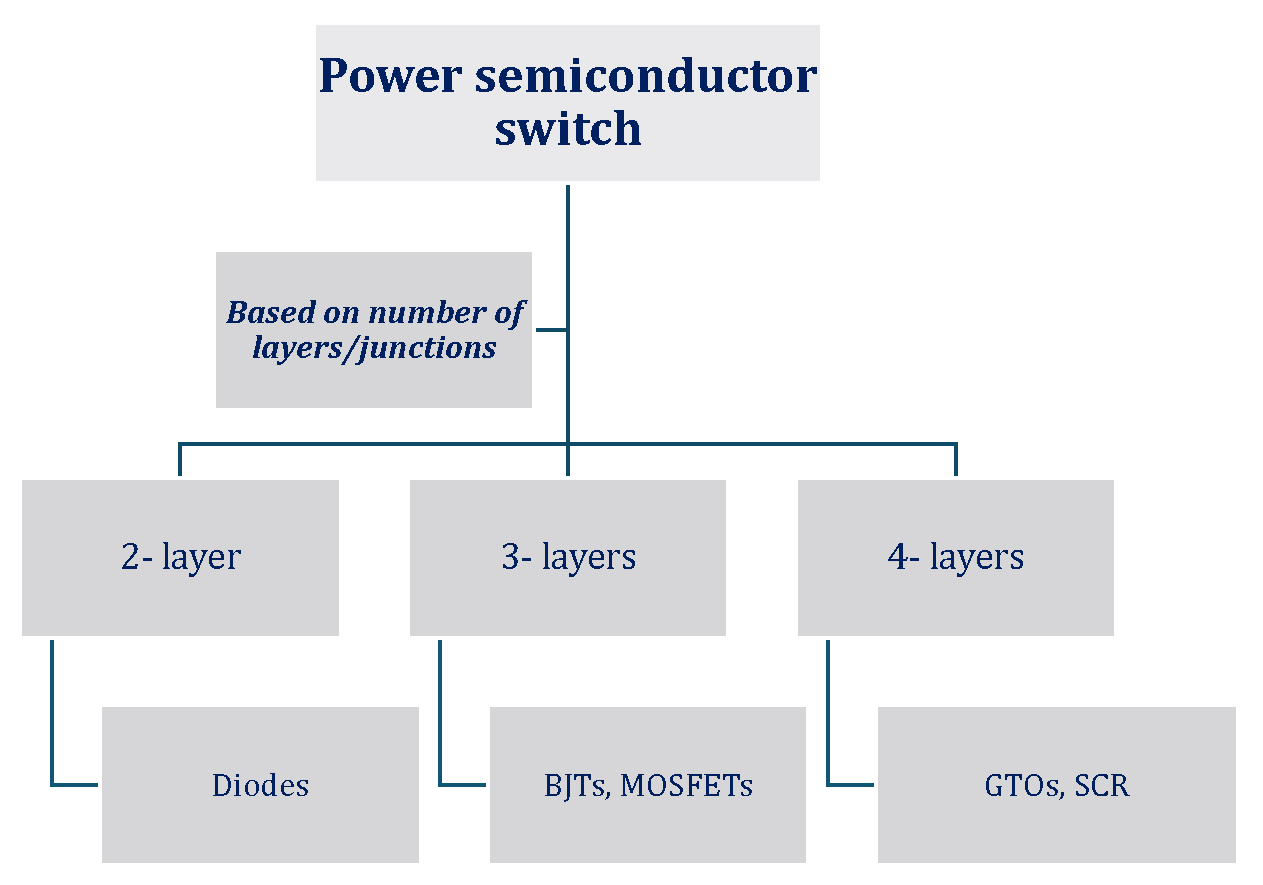
\includegraphics[scale=0.35]{fig/lec04/classification_of_device_2.eps}
            \caption{Classification of power semiconductor devices based on number of layers.}
        \end{figure}
    \end{columns}
\end{frame}

\begin{frame}
	\frametitle{Classification of types of power semiconductor devices}
    \textbf{Based on controllability:}
    \begin{columns}
        \column{0.35\textwidth}
        \begin{itemize}
            \item \textbf{Uncontrolled:}
            \begin{itemize}
                \item Diodes (e.g., Schottky, Zener, and standard rectifier diodes).
            \end{itemize}
            \item \textbf{Semicontrolled:}
            \begin{itemize}
                \item SCRs.
            \end{itemize}
            \item \textbf{Fully controlled:}
            \begin{itemize}
                \item BJTs.
                \item MOSFETs.
            \end{itemize}
        \end{itemize}

        \column{0.65\textwidth}
        \begin{figure}
            \centering
            \label{fig:Classification_based_on_controllability}
            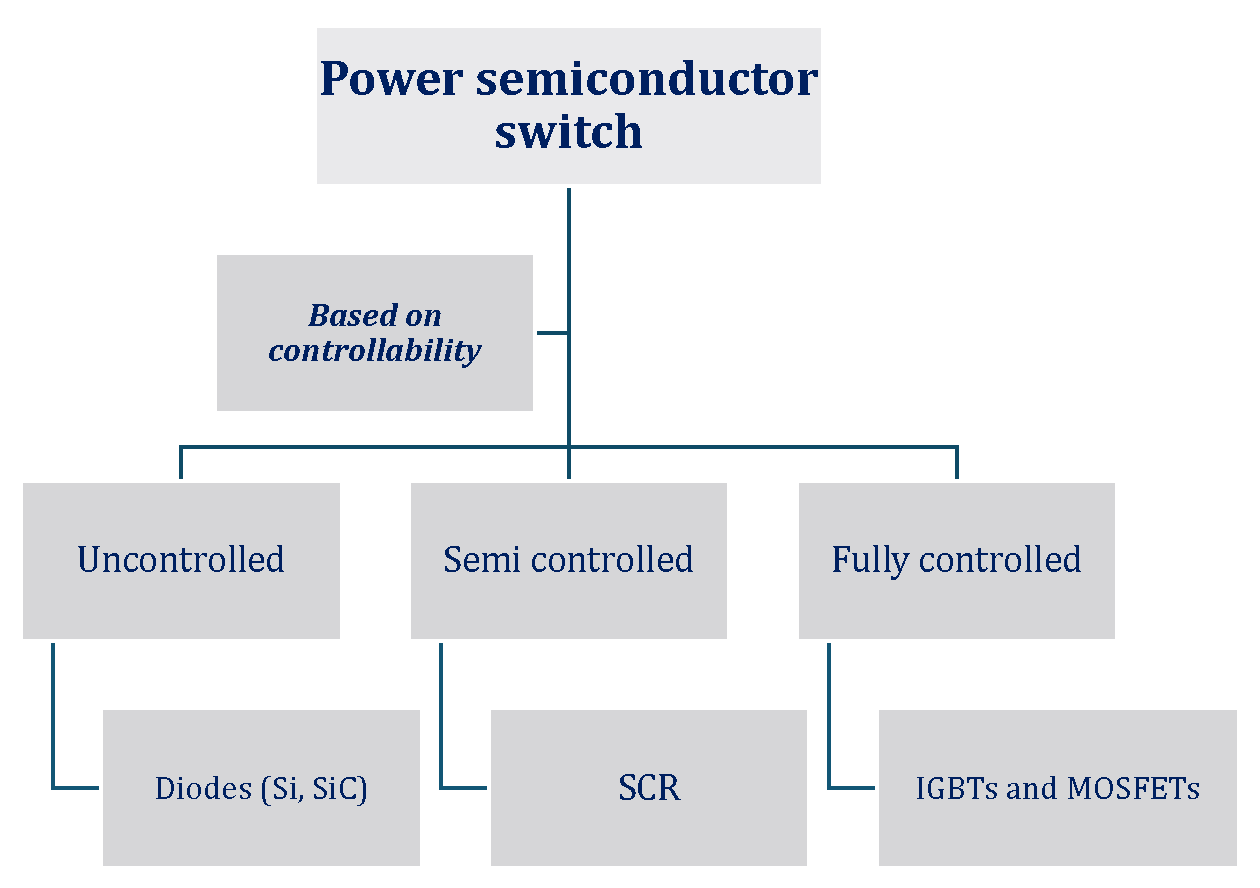
\includegraphics[scale=0.35]{fig/lec04/classification_of_device_3.eps}
            \caption{Classification of power semiconductor devices based on controllability.}
        \end{figure}
    \end{columns}
\end{frame}


\begin{frame}
	\frametitle{Classification of types of power semiconductor devices}
    \textbf{Based on quadrant of operation:}
    \begin{columns}
        \column{0.35\textwidth}
        \begin{itemize}
            \item \textbf{Single quadrant:}
            \begin{itemize}
                \item Diodes (e.g., Schottky, Zener, and standard rectifier diodes).
            \end{itemize}
            \item \textbf{Two quadrant:}
            \begin{itemize}
                \item Current bidirectional devices (e.g., MOSFETs).
                \item Voltage bidirectional devices (e.g., MOSFET with a series diodes).
            \end{itemize}
            \item \textbf{Four quadrant:}
            \begin{itemize}
                \item By combination of two or more devices (e.g., using IGBTs and MOSFETs).
                \item MOSFETs.
            \end{itemize}
        \end{itemize}

        \column{0.65\textwidth}
        \begin{figure}
            \centering
            \label{fig:Classification_based_on_quadrant_of_operation}
            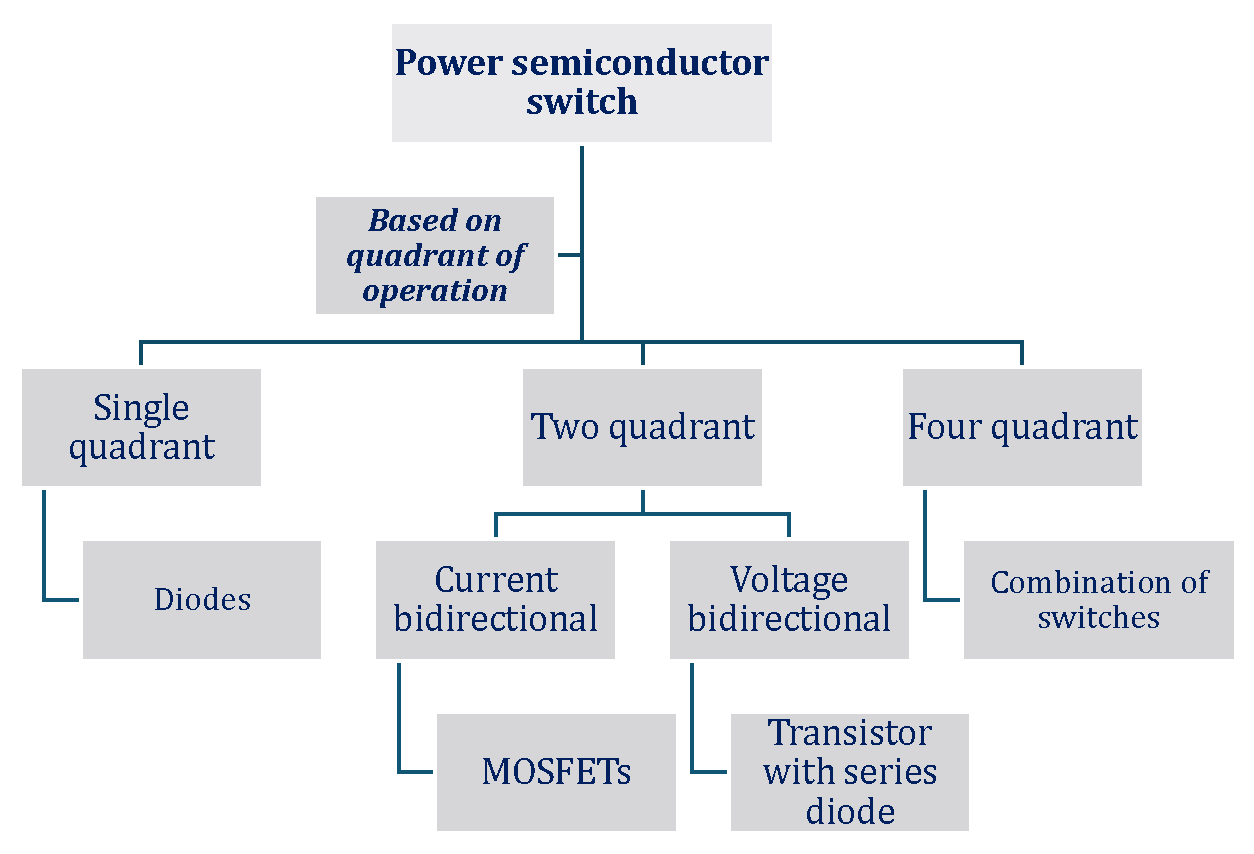
\includegraphics[scale=0.35]{fig/lec04/classification_of_device_4.eps}
            \caption{Classification of power semiconductor devices based on quadrant of operation.}
        \end{figure}
    \end{columns}
\end{frame}

%%%%%%%%%%%%%%%%%%%%%%%%%%%%%%%%%%%%%%%%%%%%%%%%%%%%%%%%%%%%%%%
%% Power Diodes %%
%%%%%%%%%%%%%%%%%%%%%%%%%%%%%%%%%%%%%%%%%%%%%%%%%%%%%%%%%%%%%%%
\begin{frame}
    \frametitle{Power Diodes}
    \textbf{1. Definition:} \\
    \textit{A power diode is a semiconductor device that allows current to flow in one direction while blocking it in the opposite direction. It is designed to handle high voltages and currents, making it suitable for power applications.}

    \textbf{2. Key Characteristics:}
    \begin{itemize}
        \item \textbf{Forward Voltage Drop (\(V_f\)):} The voltage drop across the diode when it is conducting.
        \item \textbf{Reverse Breakdown Voltage (\(V_{BR}\)):} The maximum reverse voltage the diode can withstand before breakdown occurs.
        \item \textbf{Reverse Recovery Time (\(t_{rr}\)):} The time taken for the diode to switch from conducting to blocking state.
    \end{itemize}

    \textbf{3. Types of Power Diodes:}
    \begin{itemize}
        \item \textbf{Standard Rectifier Diodes:} Used in AC-DC conversion.
        \item \textbf{Schottky Diodes:} Low forward voltage drop and fast switching; used in high-frequency applications.
        \item \textbf{Zener Diodes:} Used for voltage regulation and protection against overvoltage conditions.
    \end{itemize}
\end{frame}

\begin{frame}
    \frametitle{Power Diodes- basic structure}
    \begin{columns}
        \column{0.4\textwidth}
        \begin{itemize}
            \item \textbf{Basic Structure:}
            \begin{itemize}
                \item Inclusion of a lightly doped $n^-$ drift region.
                \begin{itemize}
                    \item the lightly doped $n^-$ layer (drift region) allows the depletion region to expand widely under reverse bias.
                    \item Allows the diode to have high voltage blocking capability
                \end{itemize}
                \item Thick epitaxial layer and high current capacity.
                \begin{itemize}
                    \item Epitaxial growth and cross-sectional area are tailored to high current rating.
                    \item Larger devices use 4-inch wafers.
                \end{itemize}
            \end{itemize}
        \end{itemize}

        \column{0.6\textwidth}
        \begin{figure}
            \centering
            \label{fig:Power_Diodes_structure_and_IV_characteristics}
            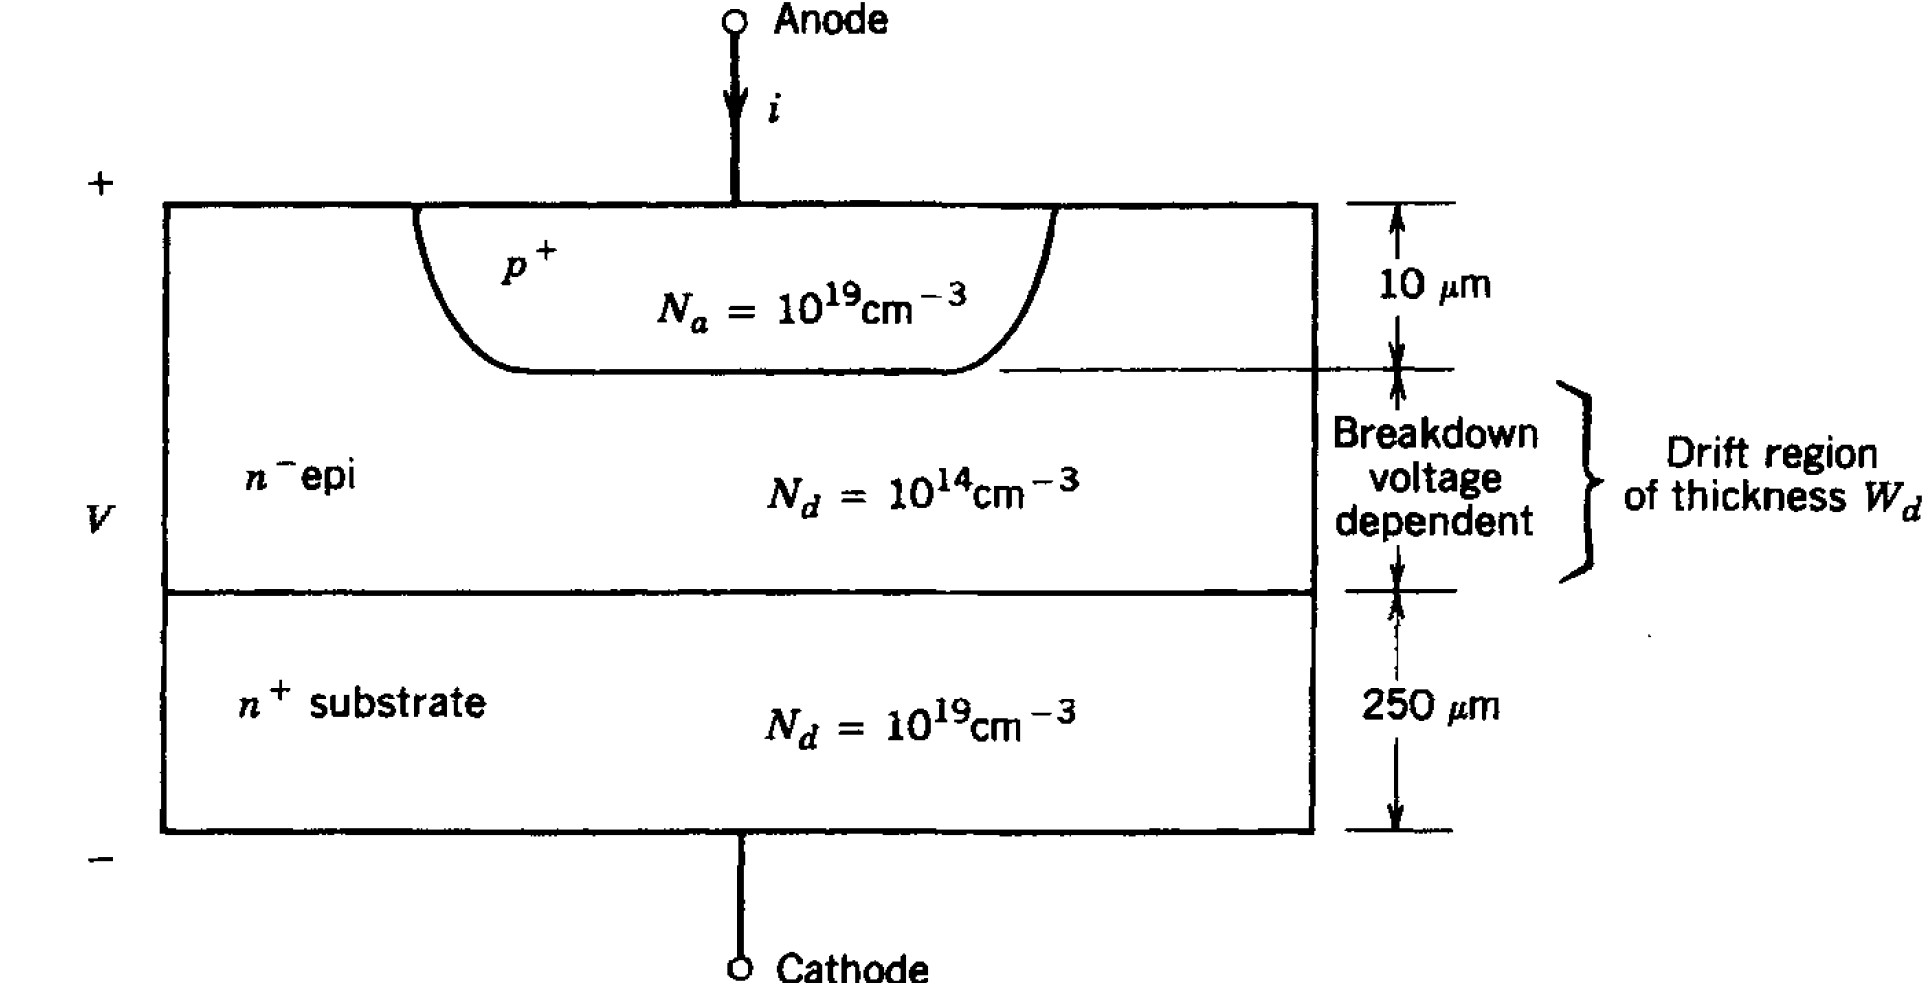
\includegraphics[scale=0.2]{fig/lec04/cross_section_pn_junction.png}
            \caption{Cross section of pn junction diode; adapted from Mohan, Undeland, Robbins, "Power Electronics: Converters, Applications and Design - 2nd Edition".}
        \end{figure}
    \end{columns}
\end{frame}

\begin{frame}
    \frametitle{Power Diodes- Static characteristics}
    \begin{columns}
        \column{0.45\textwidth}
        \begin{itemize}
            \item \textbf{Linear forward conduction:}
            \begin{itemize}
                \item high forward current flows through the lightly doped drift region, introducing significant series resistance $R_{on}$.
                \item The characteristic is linear rather than exponential beyond $\approx$ 1V.
            \end{itemize}
            \item \textbf{Reverse bias and avalanche breakdown:}
            \begin{itemize}
                \item Under reverse bias, a small leakage current flows until the breakdown voltage $BV_{BD}$ is reached.
                \item Beyond $BV_{BD}$ avalanche multiplication causes current to rise rapidly while the voltage remains approximately constant.
            \end{itemize}
            \item \textbf{Breakdown operation must be avoided!.}
        \end{itemize}

        \column{0.55\textwidth}
        \begin{figure}
            \centering
            \includegraphics[scale=0.275]{fig/lec04/static_characteristics_diode.png}
            \caption{(a) symbol of diode, (b) ideal VI characteristics, (c) VI characteristics of a practical diode (d) piece wise linear model; adapted from Umanand, L., Power Electronics: Essentials \& Applications.}
            \label{fig:static_diode_characteristics}
        \end{figure}
    \end{columns}
\end{frame}

\begin{frame}
    \frametitle{Power Diodes- Dynamic characteristics}
    \begin{columns}
        \column{0.45\textwidth}
        \textbf{Turn-OFF of Diode:}
        \begin{itemize}
            \item When a forward-biased diode is suddenly reverse biased, excess carriers in the diffusion region (space-charge region) must be removed.
            \item The diode voltage remains in the ON-state initially due to stored charge.
            \item Reverse current flows until charges are removed at time $t_2$, after which the junction becomes reverse biased.
            \item The time interval from $t_1$ to $t_2$ is termed \textbf{storage time}, and $t_{rr}$ (total duration of reverse recovery) is crucial for switching applications.
        \end{itemize}
        \column{0.55\textwidth}
        \begin{figure}
            \centering
            \includegraphics[scale=0.25]{fig/lec04/dynamic_characteristics_diode.png}
            \caption{(a) test circuit- turn-off, (b) ideal dynamic characteristics, (c) practical diode dynamic characteristics-turn-off; adapted from Umanand, L., Power Electronics: Essentials \& Applications.}
            \label{fig:dynamic_diode_characteristics}
        \end{figure}
    \end{columns}
\end{frame}

\begin{frame}
    \frametitle{Power Diodes- Dynamic characteristics}
    \begin{columns}
        \column{0.45\textwidth}
        \textbf{Turn-ON of Diode:}
        \begin{itemize}
            \item If a diode under reverse bias is forward biased, the transition requires a time known as \textbf{turn-ON time} or \textbf{forward recovery time}.
            \item Charges redistribute from to establish steady-state conduction.
            \item This process is generally faster than charge removal during turn-OFF, hence $t_{ON} < t_{OFF}$.
        \end{itemize}
        \vspace{0.2cm}
        \textit{Note: In practical circuits, reverse recovery can be slowed by parasitic inductance.}

        \column{0.55\textwidth}
        \begin{figure}
            \centering
            \includegraphics[scale=0.25]{fig/lec04/dynamic_characteristics_diode.png}
            \caption{(a) test circuit- turn-off, (b) ideal dynamic characteristics, (c) practical diode dynamic characteristics-turn-off; adapted from Umanand, L., Power Electronics: Essentials \& Applications.}
            \label{fig:dynamic_diode_characteristics}
        \end{figure}
    \end{columns}
\end{frame}

\begin{frame}{\textbf{Classification and Parameters of Power Diodes}}

    \textbf{Diode Classifications}
    \begin{itemize}
        \item Classification is based on reverse recovery time $t_{rr}$, indicating how quickly a diode can switch off.
        \item \textbf{Types of Diodes:}
        \begin{enumerate}
            \item \textbf{Rectifier Diodes:} $t_{rr}$ in the microsecond range.
            \item \textbf{Fast Recovery Diodes:} $t_{rr}$ between 200--500 ns.
            \item \textbf{Ultra-Fast Recovery Diodes:} $t_{rr} \sim$ 30--200 ns.
            \item \textbf{Schottky Diodes:} Metal-semiconductor junction, $t_{rr} <$ 30 ns.
        \end{enumerate}
        \item For high-frequency applications (e.g. SMPS, converters), use types 2--4 based on frequency and voltage ratings.
    \end{itemize}
    
    \textbf{Applications:}
    \begin{itemize}
        \item Type 1 is suitable for low-frequency mains rectification.
        \item Types 2--4 used in fast-switching converters.
    \end{itemize}
    
    \end{frame}
    
    \begin{frame}{\textbf{Datasheet Parameters for Diode Selection}}
    
    \textbf{Key Diode Parameters:}
    \begin{enumerate}
        \item Average forward current, $I_{\text{Fav}}$
        \item RMS forward current, $I_{\text{Frms}}$
        \item Peak forward current, $I_{\text{F}}$
        \item Surge current, $I_{\text{FSM}}$
        \item Breakdown or reverse voltage, $V_{\text{RRM}}$
        \item Forward voltage drop, $V_{\text{F}}$
        \item Dynamic resistance, $r_d$
        \item Reverse recovery time, $t_{rr}$
        \item Thermal endurance: $I^2t$ rating
    \end{enumerate}
    
    \textbf{Important Notes:}
    \begin{itemize}
        \item For sinusoidal operation, $I_{\text{Fav}}, I_{\text{Frms}}, I_{\text{F}}$ relations are well-known.
        \item For non-sinusoidal waveforms, these values must be derived from fundamentals.
        \item Choose diode ratings higher than the worst-case circuit values.
    \end{itemize}
    
    \end{frame}
    
    \begin{frame}{\textbf{Surge Current}}
        \textbf{Surge Current:}
        \begin{itemize}
            \item Diodes can handle overload currents briefly without damage.
            \item Key datasheet specs: $I_{\text{FSM}}$ (max peak half-cycle non-repetitive current) and $I^2t$ (energy dissipation).
            \item Surge current often arises when rectifier filters switch on with high peak voltages.
            \item Limiting devices (e.g., series resistors or fuses) ensure surge stays below $I^2t$ limit.
        \end{itemize}
    \end{frame}
        
\begin{frame}{\textbf{Thermal Viewpoint of Diodes}}
    \textbf{Thermal Viewpoint:}
    \begin{itemize}
        \item Total power loss: $P_d = P_{\text{on}} + P_{\text{off}} + P_{\text{switching}}$
        \item \textbf{On-state loss:}
        \begin{equation}
            P_{\text{on}} = \frac{1}{T} \int_0^T v(t)i(t)\, dt \approx (V_d \times I_{\text{avg}}) + (I_{\text{rms}}^2 \times r_d)
        \end{equation}
        \item \textbf{Switching loss:}
        \begin{equation}
            P_{\text{switching}} = E_{\text{switching}} \cdot f_s = \left( \frac{1}{2} Q_{\text{rr}} V_R \right) f_s
        \end{equation}
        \item Reverse recovery charge:
        \begin{equation}
            Q_{\text{rr}} = \frac{1}{2} t_{\text{rr}} I_{\text{rr}} \Rightarrow P_{\text{switching}} = \frac{1}{4} I_{\text{rr}} V_R t_{\text{rr}} f_s
        \end{equation}
        \item Junction temperature must remain below datasheet limit (e.g., 150$^\circ$C).
    \end{itemize}
\end{frame}


\begin{frame}{\textbf{Modeling a Power Diode: Steady-State and Transient Behavior}}
    \begin{columns}
        \begin{column}{0.48\textwidth}
            \textbf{Objective:} To model both static and dynamic characteristics of a diode for simulation and design purposes.
            \vspace{0.5em}
            \begin{itemize}
                \item \textbf{Steady-State Behavior:}
                \begin{itemize}
                    \item Current-voltage $(i_d$–$V_d)$ relationship is exponential:
                    \[
                        i_d = I_0\left(e^{\frac{V_d}{nV_T}} - 1\right)
                    \]
                    \item $R_s$: Series resistance due to bulk and contact resistance (non-zero in practice).
                \end{itemize}
            \end{itemize}
        \end{column}
        
        \begin{column}{0.48\textwidth}
            \begin{figure}
                \centering
                \includegraphics[scale=0.25]{fig/lec04/diode_model.png}
                \caption{Model of diode; adapted from Umanand, L., Power Electronics: Essentials \& Applications.}
                \label{fig:diode_model}
            \end{figure}
        \end{column}
    \end{columns}
    \end{frame}
    

\begin{frame}{\textbf{Modeling a Power Diode: Steady-State and Transient Behavior}}
    \begin{columns}
        \begin{column}{0.48\textwidth}
\begin{itemize}
\item \textbf{Dynamic Behavior:}
\begin{itemize}
    \item \textbf{Diffusion Capacitance ($C_D$):} 
        \begin{itemize}
            \item Appears during transition from forward to reverse bias.
            \item Models the excess mobile charge that must be removed.
        \end{itemize}
        
    \item \textbf{Transition Capacitance ($C_T$):}
        \begin{itemize}
            \item Relevant when transitioning from reverse to forward bias.
            \item Models mobile charge accumulation at the junction.
        \end{itemize}
\end{itemize}

\item \textbf{Capacitance Non-Linearity:}
    \begin{itemize}
        \item Both $C_D$ and $C_T$ are non-linear and depend on the charge distribution.
        \item Circuit simulators implement these models dynamically.
    \end{itemize}
\end{itemize}
\end{column}

\begin{column}{0.48\textwidth}
    \begin{figure}
        \centering
        \includegraphics[scale=0.25]{fig/lec04/diode_model.png}
        \caption{Model of diode; adapted from Umanand, L., Power Electronics: Essentials \& Applications.}
        \label{fig:diode_model}
    \end{figure}
\end{column}
\end{columns}
\end{frame}

\begin{frame}{\textbf{Introduction to punch-through vs non-punch-through power diodes}}
    \textbf{Differences:Punch through vs non-punch-through:} 
    \centering
    \small
    \begin{tabular}{|p{3.5cm}|p{4cm}|p{4cm}|}
    \hline
    \textbf{Characteristic} & \textbf{Punch-through (PT)} & \textbf{Non-punch-through (NPT)} \\
    \hline
    Drift Region & Thinner, moderately doped & Thicker, lightly doped \\
    \hline
    Electric Field Profile & Extends through drift region (reaches anode) & Ends before reaching the anode \\
    \hline
    Breakdown Mechanism & Abrupt avalanche breakdown & Gradual breakdown onset \\
    \hline
    Switching Speed & Faster reverse recovery & Slower but more robust \\
    \hline
    On-State Voltage Drop & Lower & Slightly higher \\
    \hline
    Reverse Recovery Loss & Lower & Higher \\
    \hline
    Application Voltage Range & Medium (e.g., 600–1200 V) & High (e.g., >1200 V) \\
    \hline
    Example Devices & Transient Voltage Suppression and Schottky barrier diodes & 1N400x  \\
    \hline
    \end{tabular} \\
    \vspace{0.3cm}
    \textbf{Design Implication:} Choice depends on switching frequency, voltage class, and thermal constraints.
\end{frame}

\begin{frame}{\textbf{Avalanche Breakdown in Step Junctions}}
    \textbf{Concept:} Reverse bias in a $p$–$n$ junction causes the electric field to drop entirely across the depletion region. As the field strength increases, it approaches a critical value $E_{\text{BD}}$ where impact ionization begins $\Rightarrow$ Avalanche Breakdown.
    
    \vspace{0.3em}
    \textbf{Key Definitions:}
    \begin{itemize}
        \item \textbf{Breakdown Voltage} ($BV_{\text{BD}}$): Reverse-bias voltage at which impact ionization becomes significant.
        \item \textbf{Critical Field Strength} ($E_{\text{BD}}$): Electric field at which avalanche multiplication starts.
    \end{itemize}
    
    \vspace{0.3em}
    \textbf{Breakdown Condition:}
    \begin{equation}
        E_{\max} \approx E_{\text{BD}}
    \end{equation}
    \textbf{Where:}
    \begin{itemize}
        \item $E_{\max}$: Maximum electric field in the depletion region.
    \end{itemize}
\end{frame}
    
\begin{frame}{\textbf{Breakdown Voltage Expression for Step Junction}}
    \begin{equation}
    BV_{\text{BD}} = \phi_c + \left[ \frac{W_0 E_{\text{BD}}}{2 \varepsilon} \right]^2 - \phi_c \approx \frac{\varepsilon (N_A + N_D) E_{\text{BD}}^2}{2 q N_A N_D}
    \end{equation}
    
    \textbf{Parameters:}
    \begin{itemize}
        \item $W_0$: Depletion width
        \item $E_{\text{BD}}$: Breakdown electric field
        \item $\varepsilon$: Permittivity of the semiconductor
        \item $N_A, N_D$: Acceptor and donor concentrations
        \item $q$: Electron charge
        \item $\phi_c$: Contact potential
    \end{itemize}
    
    \vspace{0.3em}
    \textbf{Observation:} Breakdown voltage depends strongly on doping concentrations and junction profile (e.g., step, graded, diffused).
\end{frame}


\begin{frame}{\textbf{Breakdown Voltage in Non-Punch-Through (NPT) Diodes}}

    \textbf{Structure Concept:}
    \begin{itemize}
        \item \textbf{Non-punch-through diode:} Drift region thickness $W_d$ is \textit{greater than} depletion width at breakdown.
        \item Depletion region does \textbf{not reach} the heavily doped $n^+$ substrate.
    \end{itemize}
    
    \vspace{0.4em}
    \textbf{Simplified Breakdown Voltage Equation:}
    \begin{equation}
        BV_{\text{BD}} \approx \frac{\varepsilon E_{\text{BD}}^2}{2 q N_D}
    \end{equation}
    \begin{itemize}
        \item $E_{\text{BD}}$: Breakdown electric field
        \item $N_D$: Doping concentration of drift region (lightly doped $n$)
        \item $\varepsilon$: Permittivity of the semiconductor
    \end{itemize}
    
\end{frame}

\begin{frame}{\textbf{Breakdown Voltage in Non-Punch-Through (NPT) Diodes}}

\textbf{Numerical Estimation for Silicon:}
\begin{equation}
    BV_{\text{BD}} \approx \frac{1.3 \times 10^{17}}{N_D}
\end{equation}
(for $N_D$ in $\text{cm}^{-3}$, $BV_{\text{BD}}$ in volts)

\vspace{0.4em}
\textbf{Depletion Width at Breakdown:}
\begin{equation}
    W_d \approx \frac{2 BV_{\text{BD}}}{E_{\text{BD}}} \approx 10^{-5} BV_{\text{BD}} \quad \text{(in cm)}
\end{equation}

\vspace{0.4em}
\textbf{Design Implications:}
\begin{itemize}
    \item High breakdown voltages $\Rightarrow$ require very \textbf{light doping} ($\sim 10^{14}$ cm$^{-3}$).
    \item Drift region width for 1000 V breakdown $\approx$ 100 $\mu$m.
    \item Trade-off between \textbf{blocking capability} and \textbf{on-resistance}.
\end{itemize}
\end{frame}

\begin{frame}{\textbf{Punch-Through Diode Breakdown Mechanism}}
    \begin{columns}
    
    \begin{column}{0.5\textwidth}
    \textbf{Definition:} Punch-through occurs when the reverse bias extends the depletion region entirely across the lightly doped $n^-$ drift region up to the heavily doped $n^+$ region.
    
    \begin{itemize}
        \item Reverse bias pushes the depletion edge to contact $n^+$, beyond which it cannot grow.
        \item The electric field profile changes shape — not triangular anymore.
        \item Breakdown voltage is reached when $E_1 + E_2 = E_{BD}$.
    \end{itemize}
    
    \vspace{1em}
    \textbf{Key Point:} The $n^+$ layer's heavy doping blocks further depletion region growth.
    \end{column}
    
    \begin{column}{0.5\textwidth}
    \begin{figure}
        \centering
        \includegraphics[scale=0.25]{fig/lec04/punch_through.png}
        \caption{\scriptsize Punch-through diode under reverse bias: (a) Depletion layer extends fully across the drift region (punch-through condition); (b) Electric field profile. Adapted from Mohan et al., \textit{Power Electronics, 2nd Ed.}}
        \label{fig:punch_through_diode}
    \end{figure}
    \end{column}
    
    \end{columns}
\end{frame}


\begin{frame}{\textbf{Electric Field \& Voltage Profile in Punch-Through Diode}}
    \begin{itemize}
        \item Electric field profile:
        \begin{itemize}
            \item Triangular portion: $E_1 = \frac{qN_dW_d}{\varepsilon}$
            \item Rectangular portion: $E_2$
        \end{itemize}
        \item Breakdown voltage:
        \begin{equation}
            V_1 = \frac{qN_dW_d^2}{2\varepsilon}, \quad V_2 = E_2 W_d
        \end{equation}
        \begin{equation}
            BV_{BD} = V_1 + V_2 = E_{BD}W_d - \frac{qN_dW_d^2}{2\varepsilon}
        \end{equation}
    \end{itemize}
    \textbf{Observation:} When $V_1 \ll V_2$, then $BV_{BD} \approx E_{BD}W_d$
\end{frame}

\begin{frame}{\textbf{Implications of Punch-Through Design}}
    \begin{itemize}
        \item Allows shorter $W_d$ for same $BV_{BD}$ → compact device.
        \item Higher resistivity in drift region increases $R_{on}$:
        \begin{itemize}
            \item Higher conduction loss compared to non-punch-through.
        \end{itemize}
        \item \textbf{Important:} No conductivity modulation under on-state — no conductivity injection from minority carriers.
        \item Results in higher $R_{on}$ under on-state condition.
    \end{itemize}
    \textbf{Conclusion:} Useful for high-speed, high-frequency operation despite higher on-resistance.
\end{frame}

\begin{frame}{\textbf{Schottky Diode: Structure and Principle of Operation}}
    \begin{columns}
        \begin{column}{0.6\textwidth}
        \textbf{Structure:}
        \begin{itemize}
            \item Formed by placing a metal in contact with an $n$-type semiconductor.
            \item The metal acts as the anode and the semiconductor as the cathode.
            \item Only majority carriers (electrons in $n$-type) participate — no hole injection.
        \end{itemize}
        
        \textbf{Principle of Operation:}
        \begin{itemize}
            \item Barrier formed due to work function difference.
            \item Equilibrium is reached when electron flow from metal to semiconductor balances opposite flow.
            \item No minority carriers $\Rightarrow$ no charge storage $\Rightarrow$ fast switching.
        \end{itemize}
    \end{column}
    \begin{column}{0.4\textwidth}
                \begin{figure}
                    \centering
                    \includegraphics[scale=1]{fig/lec04/schottky_diode.pdf}
                    \caption{Schottky diode structure and energy band diagram; adapted from Mohan et al., \textit{Power Electronics, 2nd Ed.}}
                    \label{fig:schottky_diode_structure}
                \end{figure}
    \end{column}
\end{columns}
\end{frame}

\begin{frame}{\textbf{I-V Characteristics of Schottky Diode}}
    \begin{columns}
        \begin{column}{0.6\textwidth}
        \textbf{Equation:}
        \begin{equation}
        I = I_s \left( e^{\frac{qV}{nkT}} - 1 \right)
        \end{equation}
        
        \textbf{Key Observations:}
        \begin{itemize}
            \item Forward drop: 0.3–0.4 V (lower than silicon $p$-$n$ junction).
            \item High reverse leakage current due to majority-carrier injection.
            \item Not suitable beyond 100–200 V breakdown.
        \end{itemize}
        \textbf{Advantage:} Very fast ON/OFF response due to absence of stored charge.
    \end{column}
    \begin{column}{0.4\textwidth}
                \begin{figure}
                    \centering
                    \includegraphics[scale=1]{fig/lec04/schottky_diode.pdf}
                    \caption{Schottky diode structure and energy band diagram; adapted from Mohan et al., \textit{Power Electronics, 2nd Ed.}}
                    \label{fig:schottky_diode_structure}
                \end{figure}
    \end{column}
\end{columns}

\end{frame}
    
\begin{frame}{\textbf{Ohmic vs Rectifying Contact in Metal–Semiconductor Junctions}}
    \textbf{Ohmic Contact:}
    \begin{itemize}
        \item No rectifying behavior; linear I-V characteristics.
        \item Occurs when metal work function $\phi_m < \phi_s$.
        \begin{itemize}
        \item The work function $\phi$ is the minimum energy needed to remove an electron from the Fermi level to vacuum.
        \item $\phi_m$ = work function of metal
        \item $\phi_s$ = work function (or electron affinity + energy gap position) of the semiconductor
    \end{itemize}
        \item Heavy doping or tunneling required to minimize barrier.
    \end{itemize}
    
    \textbf{Rectifying (Schottky) Contact:}
    \begin{itemize}
        \item Barrier prevents majority carriers $\Rightarrow$ diode action.
        \item No minority carrier injection $\Rightarrow$ low switching loss.
    \end{itemize}

\end{frame}

\begin{frame}{\textbf{Breakdown Behavior of Schottky Diodes}}
    \begin{itemize}
        \item Geometry and electric field crowding limits breakdown voltage.
        \item Surface effects and field curvature reduce breakdown to $\sim$200 V.
        \item No conductivity modulation $\Rightarrow$ higher drift region resistance.
        \item Trade-off: High $V_{BD}$ $\Rightarrow$ low doping $\Rightarrow$ high $R_{on}$.
    \end{itemize}
    \textbf{Comparison:} $p$-$n$ junction diodes can go to $\sim$5 kV due to conductivity modulation.
    \begin{itemize}
        \item Geometry and electric field crowding limits breakdown voltage.
        \item Surface effects and field curvature reduce breakdown to $\sim$200 V.
        \item No conductivity modulation $\Rightarrow$ higher drift region resistance.
        \item Trade-off: High $V_{BD}$ $\Rightarrow$ low doping $\Rightarrow$ high $R_{on}$.
    \end{itemize}
    \textbf{Comparison:} $p$-$n$ junction diodes can go to $\sim$5 kV due to conductivity modulation.
\end{frame}

\begin{frame}{\textbf{Switching Characteristics of Schottky Diodes}}
    \begin{itemize}
        \item Turn-ON and turn-OFF are extremely fast (no minority carrier storage).
        \item No reverse recovery current unlike $p$-$n$ diodes.
        \item Higher junction capacitance $\Rightarrow$ small voltage overshoot if $di/dt$ is large.
    \end{itemize}
    
    \textbf{Applications:} Preferred in high-frequency power converters and fast rectifiers. \\
    \textbf{Schottky Diode: Key Takeaways}
    \begin{itemize}
        \item Majority-carrier device with fast switching.
        \item Lower forward voltage drop (0.3–0.4 V).
        \item Poor high-voltage blocking ($<200$ V).
        \item Higher reverse leakage current than $p$-$n$ diodes.
        \item Ideal for low-voltage, high-speed power circuits.
    \end{itemize}
\end{frame}
    


\subsection{Power bipolar junction transistor (BJT)}

\begin{frame}
    \frametitle{Power bipolar junction transistor (BJT)}
    \textbf{1. Definition:} \\
    \textit{A power BJT is a three-terminal semiconductor device that can amplify or switch electronic signals and electrical power. It consists of two p-n junctions and is designed to handle high voltages and currents, making it suitable for power applications.}
\begin{itemize}
    \item Power BJTs require high blocking voltage in OFF state and high current capacity in ON state.
    \item Structure differs from logic-level BJTs to meet power handling demands.
    \item Exhibits distinct $i$–$v$ characteristics and switching behavior compared to signal BJTs.
    \item Applications include:
    \begin{itemize}
        \item Power converters
        \item Motor drives
        \item High-voltage switching circuits
    \end{itemize}
\end{itemize}
\end{frame}

\begin{frame}{\textbf{Bipolar Power Transistors (BJT)}}
\begin{itemize}
    \item BJTs are three-terminal current-controlled devices with:
    \begin{itemize}
        \item Emitter (E)
        \item Base (B)
        \item Collector (C)
    \end{itemize}
    \item Two types: \textbf{NPN} and \textbf{PNP}
    \item Current controlled: Small base current controls large collector current
    \item Can only conduct in one direction:
    \begin{itemize}
        \item NPN: C $\rightarrow$ E
        \item PNP: E $\rightarrow$ C
    \end{itemize}
    \item Structure: vertically oriented layers with heavily doped emitter and lightly doped collector
\end{itemize}
\begin{figure}
    \centering
    \includegraphics[width=0.5\linewidth]{fig/lec04/pnp_npn.png}
    \caption{BJT structure and symbol, adapted from Ned Mohan, Tore M. Undeland, and William P. Robbins, Power Electronics: Converters, Applications, and Design, 3rd Edition.}
    \label{fig:bjt_structure}
\end{figure}
\end{frame}

\begin{frame}{\textbf{Vertical Power Transistor Structure}}
    \begin{columns}
        \begin{column}{0.35\textwidth}
            \begin{itemize}
                \item 4-layer vertical structure with alternating $p$ and $n$-type regions.
                \item Base input, collector output, emitter common terminal.
                \item Vertical layout reduces $R_{\text{on}}$ and thermal resistance.
                \item Enhances current flow and reduces power dissipation.
                \item Common-emitter configuration used in power circuits.
            \end{itemize}
        \end{column}
    
        \begin{column}{0.65\textwidth}
            \begin{figure}
                \centering
                \includegraphics[scale=0.25]{fig/lec04/vertical_BJT_structure.png}
                \caption{Cross-section of a typical vertical $npn$ power BJT, adapted from Ned Mohan, Tore M. Undeland, and William P. Robbins, Power Electronics: Converters, Applications, and Design, 3rd Edition.}
            \end{figure}
        \end{column}
    \end{columns}
\end{frame}

\begin{frame}{\textbf{Doping and Thickness in Vertical BJTs}}
        \begin{columns}
        \begin{column}{0.35\textwidth}
            \begin{itemize}
                \item Emitter: Heavily doped $n^+$ ($\sim 10^{19}~\text{cm}^{-3}$)
                \item Base: Moderately doped $p$-type ($\sim 10^{16}~\text{cm}^{-3}$)
                \item Collector drift: Lightly doped $n^-$ ($\sim 10^{14}~\text{cm}^{-3}$), width = 50–200 $\mu$m
                \item Collector contact: $n^+$ ($\sim 10^{19}~\text{cm}^{-3}$)
            \end{itemize}
            \textbf{Design Considerations:}
            \begin{itemize}
                \item Base kept thin (5–20 $\mu$m) for high current gain.
                \item Drift region determines breakdown voltage.
            \end{itemize}
        \end{column}

        \begin{column}{0.65\textwidth}
            \begin{figure}
                \centering
                \includegraphics[scale=0.25]{fig/lec04/vertical_BJT_structure.png}
                \caption{Cross-section of a typical vertical $npn$ power BJT, adapted from Ned Mohan, Tore M. Undeland, and William P. Robbins, Power Electronics: Converters, Applications, and Design, 3rd Edition.}
            \end{figure}
        \end{column}
    \end{columns}
\end{frame}


\begin{frame}{\textbf{NPN Transistor: Operating Principle}}
    \begin{columns}
    \begin{column}{0.5\textwidth}
        \textbf{Operation:}
        \begin{itemize}
            \item Emitter–Base junction forward-biased $\rightarrow$ injects electrons into base.
            \item Base–Collector junction reverse-biased $\rightarrow$ collects electrons.
            \item Base is thin and lightly doped to minimize recombination.
            \item Electrons diffuse across base and are swept into collector.
            \item Base current $I_B$ is small; Collector current $I_C$ is large.
        \end{itemize}
        \textbf{Collector current:}
        \begin{equation}
            I_C = \alpha_F I_E - I_{CO}(e^{V_{CE}/V_T} - 1)
        \end{equation}
    \end{column}
    \begin{column}{0.5\textwidth}
        \begin{figure}
            \centering
            \includegraphics[width=0.8\linewidth]{fig/lec04/npn_bjt_operation.png}
            \caption{NPN BJT operation under forward active mode; adapted from Mohan et al., \textit{Power Electronics, 2nd Ed.}}
            \label{fig:npn_bjt_operation}
        \end{figure}
        \textbf{Emitter current:}
        \begin{equation}
        I_E = \alpha_R I_C - I_{EO}(e^{V_{EC}/V_T} - 1)
        \end{equation}
    \end{column}
  \end{columns}
\end{frame}

\begin{frame}{\textbf{BJT Current Components and Ebers-Moll Model}}
        \begin{columns}
    \begin{column}{0.4\textwidth}
        \begin{itemize}
            \item BJT modeled using Ebers-Moll equivalent circuit
            \item Includes forward and reverse $\alpha$ parameters
            \item Defines base, collector, and emitter currents via diode current equations
        \end{itemize}
        \begin{align*}
        I_C &= \alpha_F I_F - I_{CO}(e^{V_{CE}/V_T} - 1) \\
        I_E &= \alpha_R I_R - I_{EO}(e^{V_{EC}/V_T} - 1)
        \end{align*}
        \textbf{Current continuity:} $I_C + I_E + I_B = 0$
    \end{column}
    \begin{column}{0.6\textwidth}
        \begin{figure}
            \centering
            \includegraphics[width=0.8\linewidth]{fig/lec04/NPN_BJT_eq_model.png}
            \caption{Ebers-Moll equivalent circuit of NPN BJT}
        \end{figure}
    \end{column}
  \end{columns}
\end{frame}

\begin{frame}{\textbf{Key Parameters and Insights}}
\begin{itemize}
    \item $\alpha_F = \frac{I_C}{I_E}$ (forward common-base current gain), typically 0.9 to 0.98
    \item $\alpha_R = \frac{I_E}{I_R}$ (reverse common-base current gain), typically 0.02 to 0.1
    \item $\alpha_R$ is usually much smaller than $\alpha_F$.
    \item $\beta = \frac{I_C}{I_B}$ (common-emitter current gain), typically 50 to 200
    \item Higher $\alpha$ → better carrier injection from emitter
    \item Thin base → high efficiency but increased risk of punch-through
    \item $I_B$ is small but essential for switching control
\end{itemize}
\vspace{0.5em}
\textbf{Conclusion:} BJT operates via minority carrier injection and diffusion under strong forward bias conditions. It is highly efficient for amplification and switching when designed with proper base width and doping gradients.
\end{frame}


\begin{frame}{\textbf{BJT Current Gain Mechanism and Base Transport}}
\begin{columns}
\begin{column}{0.6\textwidth}
\textbf{Active Region Operation:}
\begin{itemize}
    \item In the active mode of a BJT, the base-emitter junction is forward biased, and the base-collector junction is reverse biased.
    \item Electrons are injected from the emitter (n$^+$) into the base (p) and then diffuse toward the collector.
    \item The base is intentionally kept very thin and lightly doped to minimize recombination and ensure most electrons reach the collector.
    \item The resulting collector current $I_C$ is almost equal to the emitter current $I_E$, while the base current $I_B$ remains small.
\end{itemize}

\textbf{Implication:} The small base current and large collector current results in current gain $\beta = \frac{I_C}{I_B}$.
\end{column}

\begin{column}{0.4\textwidth}
\begin{figure}
    \centering
    \includegraphics[width=1\textwidth]{fig/lec04/cross_section_BJT.png}
    \caption{Simplified cross-sectional model of BJT and current components; adapted from Ned Mohan, Tore M. Undeland, and William P. Robbins, Power Electronics: Converters, Applications, and Design, 3rd Edition.}
\end{figure}
\end{column}
\end{columns}
\end{frame}


\begin{frame}{\textbf{Diffusion Currents and Stored Charge Distribution}}
\begin{columns}
\begin{column}{0.6\textwidth}
\begin{itemize}
    \item The injected electrons from the emitter diffuse through the base to the collector, supported by the electric field across the reverse-biased base-collector junction.
    \item Recombination in the base is minimized due to short base width and high diffusion constant.
    \item Stored charge distribution within the base and collector regions affects dynamic response and switching.
    \item The base current includes three components:
    \begin{itemize}
        \item $I_{ne}$: diffusion of electrons injected from emitter to base.
        \item $I_{nc}$: recombination in the collector depletion layer.
        \item $I_{pe}$: holes injected into emitter to maintain charge neutrality.
    \end{itemize}
\end{itemize}
\end{column}

\begin{column}{0.4\textwidth}
\begin{figure}
    \centering
    \includegraphics[width=1\textwidth]{fig/lec04/stored_charge_BJT.png}
    \caption{Stored charge vs. log(p,n) profile; adapted from Ned Mohan, Tore M. Undeland, and William P. Robbins, Power Electronics: Converters, Applications, and Design, 3rd Edition.}
\end{figure}
\end{column}
\end{columns}
\end{frame}


\begin{frame}{\textbf{Expression for Current Gain and Beta}}
    \begin{columns}
\begin{column}{0.65\textwidth}
\textbf{Terminal Current Definitions:}
\begin{equation}
\begin{aligned}
I_C &= I_{nc} \\
I_E &= I_{ne} + I_{pe} \\
I_B &= I_E - I_C = I_{ne} - I_{nc} + I_{pe}
\end{aligned}
\end{equation}
\textbf{Gain Expression:}
\begin{equation}
\frac{I_B}{I_C} = \frac{I_{ne} - I_{nc}}{I_{nc}} + \frac{I_{pe}}{I_{nc}} \Rightarrow \beta = \left( \frac{I_B}{I_C} \right)^{-1}
\end{equation}
\textbf{Optimization:}
\begin{itemize}
    \item Large $\beta$ requires: small $I_{pe}$ (via heavy emitter doping), minimal $(I_{ne} - I_{nc})$ (via long electron lifetime in base).
    \item Thin base to reduce recombination path and ensure efficient electron diffusion.
\end{itemize}
\end{column}

\begin{column}{0.35\textwidth}
\begin{figure}
    \centering
    \includegraphics[width=1\textwidth]{fig/lec04/BJT_Current_gain_plot.png}
    \caption{Variation of BJT $\beta$ and $V_{CE(sat)}$, as a function of dc collector current; adapted from Ned Mohan, Tore M. Undeland, and William P. Robbins, Power Electronics: Converters, Applications, and Design, 3rd Edition.}
\end{figure}
\end{column}
\end{columns}
\end{frame}


\begin{frame}{\textbf{Emitter Current Crowding and its Impact on Beta}}
\begin{columns}
\begin{column}{0.6\textwidth}
\begin{itemize}
    \item Emitter current does not flow uniformly due to geometry and lateral resistance in the base.
    \item The voltage drop across the base-emitter junction is higher near the emitter edge, leading to current crowding.
    \item Result: Increased base current density at the emitter edge $\Rightarrow$ early onset of high-level injection $\Rightarrow$ fall in $\beta$.
    \item Modern power BJTs mitigate this by using interleaved emitter-base finger structures.
\end{itemize}
\end{column}

\begin{column}{0.4\textwidth}
\begin{figure}
    \centering
    \includegraphics[width=0.6\textwidth]{fig/lec04/BJT_current_crowding.png}
    \caption{Forward-biased emitter current crowding due to lateral base resistance; adapted from Ned Mohan, Tore M. Undeland, and William P. Robbins, Power Electronics: Converters, Applications, and Design, 3rd Edition.}
\end{figure}
\end{column}
\end{columns}
\end{frame}


\begin{frame}{\textbf{Quasi-Saturation in Power BJTs}}
\begin{columns}
\begin{column}{0.55\textwidth}
\begin{itemize}
    \item At high $I_C$, the voltage drop across the drift region increases due to $R_d$.
    \item The base-collector junction becomes weakly forward biased.
    \item Hole injection from base to collector drift occurs, and space-charge neutrality requires electron injection as well.
    \item Drift region begins to accumulate charge on one side only — this is quasi-saturation.
\end{itemize}

\begin{equation}
i_C = \frac{V_{CE}}{R_d}
\end{equation}
\end{column}

\begin{column}{0.45\textwidth}
\begin{figure}
    \centering
    \includegraphics[width=0.5\textwidth]{fig/lec04/BJT_stored_charge_distribution.png}
    \caption{Charge profile showing virtual base in quasi-saturation; adapted from Ned Mohan, Tore M. Undeland, and William P. Robbins, Power Electronics: Converters, Applications, and Design, 3rd Edition.}
\end{figure}
\end{column}
\end{columns}
\end{frame}


\begin{frame}{Static Characteristics of BJT}
    \begin{columns}
    \begin{column}{0.55\textwidth}
    \begin{itemize}
        \item A BJT is a current-controlled device.
        \item Its output characteristic $i_C$ versus $V_{CE}$ depends on the base current $i_B$:
        \[
            i_C = f(V_{CE}, i_B)
        \]
        \item The collector current is ideally $i_C = \beta i_B$, where $\beta$ is the current gain of the transistor.
        \item However, due to the Early effect (modulation of base width with $V_{CE}$), $\beta$ is not constant.
        \item This leads to variation in $i_C$ for the same $i_B$ as $V_{CE}$ increases.
    \end{itemize}
    \end{column}

    \begin{column}{0.45\textwidth}
    \begin{figure}
        \centering
        \includegraphics[width=1\textwidth]{fig/lec04/BJT_eq_circuit.png}
        \caption{BJT equivalent circuit with resistances and capacitances; ; adapted from Mohan et al., \textit{Power Electronics, 2nd Ed.}}
    \end{figure}
    \end{column}
\end{columns}
\end{frame}


\begin{frame}{Output Characteristics of a Transistor}
    \begin{columns}
    \begin{column}{0.55\textwidth}
    \begin{itemize}
        \item The $i_C$ vs $V_{CE}$ curve reveals three operating regions:
        \begin{enumerate}
            \item \textbf{Saturation Region:} Very low $V_{CE}$, high $i_C$, transistor fully ON.
            \item \textbf{Active Region:} $i_C \approx \beta i_B$, transistor used for amplification.
            \item \textbf{Cutoff Region:} $i_B \approx 0$, thus $i_C \approx 0$, transistor OFF.
        \end{enumerate}
        \item The Load Line on the output characteristic intersects the $i_C$-$V_{CE}$ curves based on $i_B$.
        \item Used to find the Q-point in analog design.
    \end{itemize}
    \end{column}

    \begin{column}{0.45\textwidth}
        \begin{figure}
        \centering
        \includegraphics[width=1\textwidth]{fig/lec04/BJT_VI_Characteristics.png}
        \caption{Output characteristics of a BJT; adapted from Umanand, L., \textit{Power Electronics, Essentials and Applications.}}
    \end{figure}
    \end{column}
\end{columns}
\end{frame}


\begin{frame}{Power BJT – Static Characteristics}
    \begin{columns}
    \begin{column}{0.6\textwidth}

    \begin{itemize}
        \item Power BJTs exhibit similar $i_C$-$V_{CE}$ behavior but with effects like:
        \begin{itemize}
            \item \textbf{Quasi-saturation:} due to the lightly doped collector drift region.
            \item \textbf{Second breakdown:} due to localized thermal hotspots under high $i_C$.
        \end{itemize}
        \item Three major regions are:
        \begin{enumerate}
            \item Active region: Used for amplification.
            \item Quasi-saturation: Forward-biased $C$-$B$ junction begins to conduct.
            \item Hard saturation: Excess carrier injection across drift region.
        \end{enumerate}
        \item Breakdown voltages:
        \begin{itemize}
            \item $BV_{CBO}$: Collector-base with emitter open.
            \item $BV_{CEO}$: Collector-emitter with base open.
            \item $BV_{SUS}$: Sustaining voltage after breakdown onset.
        \end{itemize}
    \end{itemize}
    \end{column}

    \begin{column}{0.4\textwidth}
    \begin{figure}
        \centering
        \includegraphics[width=0.8\textwidth]{fig/lec04/BJT_VI_Characteristics2.png}
        \caption{$i_C$-$V_{CE}$ curves with $I_B$ steps; adapted from Ned Mohan, Tore M. Undeland, and William P. Robbins, Power Electronics: Converters, Applications, and Design, 3rd Edition.}
    \end{figure}
    \end{column}
\end{columns}
\end{frame}

\begin{frame}{Current Gain and Load Line Intersection}
    \begin{columns}
    \begin{column}{0.6\textwidth}
    \begin{itemize}
        \item For a given $i_B$, collector current $i_C = \beta i_B$ in the active region.
        \item $\beta$ is affected by:
        \begin{itemize}
            \item Injection efficiency (related to emitter doping)
            \item Base transport factor (related to recombination and diffusion in base)
        \end{itemize}
        \item Load line defined by:
        \[
            i_C = \frac{V_{CC} - V_{CE}}{R_L}
        \]
        \item Intersection of load line and transistor characteristic determines Q-point.
    \end{itemize}
    \end{column}

    \begin{column}{0.4\textwidth}
    \begin{figure}
        \centering
        \includegraphics[width=0.8\textwidth]{fig/lec04/BJT_VI_Characteristics2.png}
        \caption{$i_C$-$V_{CE}$ curves with $I_B$ steps; adapted from Ned Mohan, Tore M. Undeland, and William P. Robbins, Power Electronics: Converters, Applications, and Design, 3rd Edition.}
    \end{figure}
    \end{column}
\end{columns}
\end{frame}


\begin{frame}{Key Observations in Power BJT Static Behavior}
    \begin{columns}
    \begin{column}{0.6\textwidth}
    \begin{itemize}
        \item Unlike small-signal BJTs, power BJTs show:
        \begin{itemize}
            \item \textbf{Lower current gain $\beta$}, especially in quasi-saturation.
            \item \textbf{Voltage fall-off due to second breakdown.}
            \item \textbf{Load line may enter second breakdown zone}, leading to thermal failure.
        \end{itemize}
        \item Quasi-saturation is due to double carrier injection in the collector drift region.
        \item Proper thermal and current limiting design is critical in power BJTs.
    \end{itemize}
    \end{column}

    \begin{column}{0.4\textwidth}
    \begin{figure}
        \centering
        \includegraphics[width=0.8\textwidth]{fig/lec04/BJT_VI_Characteristics2.png}
        \caption{$i_C$-$V_{CE}$ curves with $I_B$ steps; adapted from Ned Mohan, Tore M. Undeland, and William P. Robbins, Power Electronics: Converters, Applications, and Design, 3rd Edition.}
    \end{figure}
    \end{column}
\end{columns}
\end{frame}



\begin{frame}{Dynamic Characteristics of BJT}
\textbf{In the ON-state, a transistor stores three main charges:}
\begin{enumerate}
    \item \textbf{$Q_b$}: Charge stored in the base region.
    \item \textbf{$Q_{ce}$}: Charge in the collector region beneath the emitter.
    \item \textbf{$Q_{cb}$}: Charge in the collector region beneath the base contact.
\end{enumerate}

\vspace{1em}
These charges define the transient behavior during switching. When transitioning to the OFF-state, all three must be removed for the transistor to fully block current.

\begin{figure}
    \centering
    % \includegraphics[width=0.7\linewidth]{your_figure_path}
    \caption{[Add diagram showing positions of $Q_b$, $Q_{ce}$, and $Q_{cb}$]}
\end{figure}
\end{frame}


\begin{frame}{Charge Dependency on $V_{CE}$ and $I_C$}
        \begin{columns}
    \begin{column}{0.5\textwidth}
\begin{itemize}
    \item \textbf{$Q_b$} is largely independent of $V_{CE}$, but increases with $I_C$.
    \item \textbf{$Q_{ce}$} increases with $I_C$ but decreases as $V_{CE}$ increases.
    \item \textbf{$Q_{cb}$} grows rapidly as $V_{CE}$ drops — marking the onset of saturation.
\end{itemize}

\textbf{Implication:} Charge buildup significantly affects collector-emitter voltage and switching speed.
    \end{column}

    \begin{column}{0.5\textwidth}
\begin{figure}
    \centering
    \includegraphics[width=1\linewidth]{fig/lec04/BJT_charge_dependancy.png}
    \caption{$Q$ vs $V_{CE}$ and $Q$ vs $I_C$; adapted from Umanand, L., \textit{Power Electronics, Essentials and Applications.}}
\end{figure}
    \end{column}
\end{columns}
\end{frame}


\begin{frame}{Turn-OFF of BJT – Physical Process}
  \begin{columns}
    \begin{column}{0.5\textwidth}
\begin{itemize}
    \item Turn-off begins when base drive is removed or reversed.
    \item $Q_b$ is removed first, starting from edges near the emitter.
    \item $Q_{ce}$ and $Q_{cb}$ follow, shrinking towards the center.
    \item Residual charge $Q_r$ creates a \textit{tail current}, affecting turn-off time.
\end{itemize}
\textbf{Storage time $t_s$}: Time during which current still flows due to residual charge even after base drive is removed.
    \end{column}

    \begin{column}{0.5\textwidth}
\begin{figure}
    \centering
    \includegraphics[width=0.65\linewidth]{fig/lec04/BJT_turn_off.png}
    \caption{BJT Turn-off process: charge removal sequence; adapted from Umanand, L., \textit{Power Electronics, Essentials and Applications.}}
\end{figure}
    \end{column}
\end{columns}
\end{frame}


\begin{frame}{Turn-ON of BJT – Dynamics}
  \begin{columns}
    \begin{column}{0.5\textwidth}
\begin{itemize}
    \item In OFF-state, there are no stored charges.
    \item A positive base pulse injects $Q_{ce}$, reducing $V_{CE}$ rapidly.
    \item A sharp peak in base current is ideal for quick charge buildup.
    \item Faster ON-switching means lower energy loss.
\end{itemize}

\textbf{Switching losses during turn-ON} depend on:
\begin{itemize}
    \item Time to establish $Q_{ce}$ and $Q_b$.
    \item Load characteristics (resistive or inductive).
\end{itemize}
    \end{column}

    \begin{column}{0.5\textwidth}
\begin{figure}
    \centering
    \includegraphics[width=0.5\linewidth]{fig/lec04/BJT_turn_on.png}
    \caption{BJT Turn-on process: charge buildup sequence; adapted from Umanand, L., \textit{Power Electronics, Essentials and Applications.}}
\end{figure}
    \end{column}
\end{columns}
\end{frame}



\begin{frame}{Power Dissipation in BJT}
\textbf{Total Power Dissipation:}
\[
P_d = P_{on} + P_{off} + P_{switching}
\]

\textbf{ON-state Loss:}
\[
P_{on} = V_{CE(sat)} \times I_C \times D
\]
where $D$ is the duty cycle.

\textbf{Switching Loss (OFF $\rightarrow$ ON):}
\[
P_{\text{OFF-ON}} = \frac{V_{cc} I_C t_f f_s}{6}
\]

\textbf{Switching Loss (ON $\rightarrow$ OFF):}
\[
P_{\text{ON-OFF}} = \frac{V_{cc} I_C t_r f_s}{6}
\]

\textbf{Total Switching Loss:}
\[
P_{\text{switching}} = \frac{V_{cc} I_C f_s (t_r + t_f)}{6}
\]
\end{frame}


\begin{frame}{Safe Operating Area (SOAR)}
      \begin{columns}
    \begin{column}{0.5\textwidth}
\textbf{SOAR}: Region where transistor operates safely under given voltage-current conditions.

\begin{itemize}
    \item Forward SOAR (FSOAR): With positive base drive.
    \item Reverse SOAR (RSOAR): With negative base drive (turn-off).
    \item Delimits power dissipation, collector voltage, and current density.
\end{itemize}

\textbf{Key Constraints:}
\begin{itemize}
    \item Second breakdown limit.
    \item Thermal limits (hot spot prevention).
    \item Switching-induced crowding.
\end{itemize}
    \end{column}

    \begin{column}{0.5\textwidth}
\begin{figure}
    \centering
    \includegraphics[width=0.8\linewidth]{fig/lec04/BJT_SOAR_RSOAR.png}
    \caption{SOAR and RSOAR curves for a power BJT; adapted from Umanand, L., \textit{Power Electronics, Essentials and Applications.}}
\end{figure}
    \end{column}
\end{columns}
\end{frame}


%------------------------------------------------

\begin{frame}{Breakdown Voltages in BJTs}
\begin{itemize}
  \item In the blocking state, the C--B junction must withstand the applied voltage.
  \item The B--E junction has a lower breakdown voltage (5–20 V) due to heavy emitter doping to achieve high $\beta$.
  \item To withstand high voltages, a lightly doped collector drift region is used.
  \item Base width is minimized to maintain gain but limited to avoid reach-through breakdown.
\end{itemize}
\vspace{0.5em}
\textbf{Design Trade-off:} Thin base for high gain vs. thick base for high voltage.
\textbf{Breakdown Voltage Expressions:}
\begin{itemize}
  \item In common-emitter configuration: $BV_{CEO} < BV_{CBO}$
  \item Relationship:
  \[
  BV_{CEO} = \frac{BV_{CBO}}{\beta^{1/n}} \quad \text{where } n = 4 \text{ for } npn, n = 6 \text{ for } pnp
  \]
  \item Due to reverse-bias current $I_{CBO}$ at B--E junction, impact ionization rate increases in emitter-open mode.
\end{itemize}
\end{frame}

%------------------------------------------------

\begin{frame}{Second Breakdown, Thermal Runaway and Localized Hotspots}
\begin{itemize}
  \item Occurs at high $V_{CE}$ and $I_C$ despite staying below primary breakdown.
  \item Triggered by localized thermal runaway and current filamentation.
  \item Exponential increase in power dissipation with temperature due to:
  \[
  n_i \propto \exp\left(-\frac{E_g}{2kT}\right)
  \]
  \item Dangerous due to steep $V_{CE}$ drop and rapid localized heating.
\end{itemize}
\textbf{Thermal Runaway and Localized Hotspots}
\begin{itemize}
  \item Filamentation: nonuniform current density leads to $J_A > J_B$
  \item Result: $T_A > T_B$ $\Rightarrow$ runaway due to positive feedback
  \item Region A may exceed intrinsic temperature $T_i$ causing catastrophic failure.
  \item Preventive measures:
  \begin{itemize}
    \item Use of snubbers and freewheeling diodes.
    \item Narrow emitter stripes.
    \item Controlled $di/dt$ and $dv/dt$ during switching.
  \end{itemize}
\end{itemize}
\end{frame}

%------------------------------------------------

\begin{frame}{On-State Losses}
    \begin{columns}
        \begin{column}{0.5\textwidth}
            \begin{itemize}
                \item Dominated by conduction loss:
                \[
                P_{on} = I_C \cdot V_{CE(sat)}
                \]
                \item $V_{CE(sat)}$ increases with $I_C$ due to:
                \[
                V_{CE(sat)} = V_{BE(on)} - V_{BC(sat)} + V_d + I_C(R_e + R_c)
                \]
                \item Main contributor: $V_d$ across collector drift region.
                \item $V_d$ depends on carrier lifetime; trade-off between low $V_d$ and fast switching.
            \end{itemize}
        \end{column}

\begin{column}{0.5\textwidth}
\begin{figure}
\centering
\includegraphics[width=0.6\textwidth]{fig/lec04/BJT_on_state_losses.png}
\caption{On-state losses in a BJT; adapted from Umanand, L., \textit{Power Electronics, Essentials and Applications.}}
\label{fig:bjt_on_state_losses}
\end{figure}
    \end{column}
    \end{columns}
\end{frame}

%------------------------------------------------

\begin{frame}{Paralleling of BJTs}
        \begin{columns}
        \begin{column}{0.5\textwidth}
\begin{itemize}
  \item Used in high-current applications to share load.
  \item Risk: thermal runaway due to negative temp. coeff. of $V_{BE}$.
  \item Solution: Add emitter resistance $R$ for negative feedback.
  \[
  V_{be1} = V_{be2} + R(I_{c1} - I_{c2}) \Rightarrow \Delta V_{be} = R \Delta I_c
  \]
  \item Limit $\Delta V_{be}$ to $\approx$ 0.2 V to allow $\Delta I_C \leq 0.5$ A.
\end{itemize}
        \end{column}

\begin{column}{0.5\textwidth}
\begin{figure}
\centering
\includegraphics[width=0.6\textwidth]{fig/lec04/BJT_parallel.png}
\caption{Paralleling of BJT; adapted from Umanand, L., \textit{Power Electronics, Essentials and Applications.}}
\label{fig:bjt_on_state_losses}
\end{figure}
    \end{column}
    \end{columns}
\end{frame}

%------------------------------------------------

\begin{frame}{Darlington Connection}
            \begin{columns}
        \begin{column}{0.5\textwidth}
\begin{itemize}
  \item Used to boost current gain:
  \[
  I_B = \frac{I_C}{\beta_1 \cdot \beta_2}
  \]
  \item Higher $V_{CE(sat)} \approx$ 1–1.2 V compared to 0.4–0.6 V for single BJT.
  \item Ideal for high-power applications where base drive must be minimized.
  \item Trade-off: higher power loss and slower switching.
\end{itemize}
        \end{column}

\begin{column}{0.5\textwidth}
\begin{figure}
\centering
\includegraphics[width=0.6\textwidth]{fig/lec04/darlington_BJTs.png}
\caption{Darlington; adapted from Umanand, L., \textit{Power Electronics, Essentials and Applications.}}
\label{fig:bjt_on_state_losses}
\end{figure}
    \end{column}
    \end{columns}
\end{frame} % Introduction to power semiconductor devices
%\section{Conventional Power Semiconductor Devices}
\title{Conventional Power Semiconductor Devices}  

\begin{frame}[plain]
    \titlepage
\end{frame}

%%%%%%%%%%%%%%%%%%%%%%%%%%%%%%%%%%%%%%%%%%%%%%%%%%%%%%%%%%%%%
%% Homopolar / unipolar machines %%
%% Planned topics: Power MOSFETs, IGBTs, Thyristors %%
%%%%%%%%%%%%%%%%%%%%%%%%%%%%%%%%%%%%%%%%%%%%%%%%%%%%%%%%%%%%%
\begin{frame}{Introduction to Power MOSFETs}
\begin{itemize}
    \item Power MOSFETs (Metal-Oxide-Semiconductor Field Effect Transistors) are widely used in power electronics since the early 1980s.
    \item They offer high on-state current capability and off-state voltage blocking, making them suitable for high-speed switching applications.
    \item Replacing BJTs in many applications, especially those requiring fast switching, due to their voltage-controlled nature.
    \item Understanding the differences between BJTs and MOSFETs is crucial for effective circuit design.
    \item This section introduces the physical structure, voltage and current limits, and failure mechanisms of MOSFETs.
\end{itemize}

\vspace{0.5cm}
\textbf{Figure Placeholder:} \textit{Power MOSFET application context diagram (optional).}
\end{frame}


\begin{frame}{Basic Structure of Power MOSFET}
\begin{itemize}
    \item The MOSFET is constructed with alternating p-type and n-type layers: \textbf{n$^+$-p-n$^-$-n$^+$}.
    \item The n$^+$ (source and drain), p-body, and n$^-$ (drift region) form the core active structure.
    \item Gate terminal is insulated from the body by silicon dioxide (SiO$_2$) forming the gate oxide.
    \item Applying a positive voltage to the gate induces an n-channel in the p-body, allowing current flow.
    \item The drift region (n$^-$) is lightly doped to handle high blocking voltages.
\end{itemize}

\vspace{0.5cm}
\textbf{Figure Placeholder:} \textit{MOSFET cross-section with labels for source, gate, drain, body, and drift region.}
\end{frame}

\begin{frame}{Perspective View of a Power MOSFET}
\begin{itemize}
    \item Power MOSFETs consist of thousands of small identical cells connected in parallel.
    \item Each cell includes source diffusion, gate conductor, field oxide, and drain contact.
    \item High current handling is achieved by maximizing the number of cells and gate width.
    \item This configuration is often referred to as VDMOS (Vertical Diffused MOSFET).
    \item Parasitic elements like a BJT and integral body diode are naturally formed.
\end{itemize}

\vspace{0.5cm}
\textbf{Figure Placeholder:} \textit{Figure 22-1(b): Perspective structure showing MOSFET cellular layout.}
\end{frame}

\begin{frame}{Channel Formation and Operation}
\begin{itemize}
    \item The p-body prevents current flow until a gate voltage is applied.
    \item Applying V$_{GS} > V_{th}$ induces an n-channel in the p-body.
    \item This connects the source to the drain allowing electron flow (n-channel enhancement).
    \item No minority carrier injection occurs—enabling fast switching.
    \item The MOSFET operates as a unidirectional voltage-controlled switch.
\end{itemize}

\vspace{0.5cm}
\textbf{Figure Placeholder:} \textit{Figure 22-2(a): Accumulation layer in ON-state.}
\end{frame}

\begin{frame}{Gate Metallization and Field Plate Action}
\begin{itemize}
    \item Gate metallization overlaps the n$^-$ drift region to serve two purposes:
    \begin{enumerate}
        \item Enhances conductivity during ON-state by forming accumulation layer.
        \item Acts as a field plate to reduce electric field curvature in OFF-state.
    \end{enumerate}
    \item This helps to minimize on-resistance and improves breakdown voltage.
    \item Design strategies include optimizing gate width-to-length ratio to maximize gain.
\end{itemize}

\vspace{0.5cm}
\textbf{Figure Placeholder:} \textit{Figure 22-2(b): Field plate action during OFF-state.}
\end{frame}


\begin{frame}{Inversion Layers and the Field Effect}
\begin{itemize}
    \item The gate region of the MOSFET is composed of:
    \begin{itemize}
        \item Gate metallization (e.g., Al or polysilicon)
        \item Gate oxide ($SiO_2$)
        \item Silicon substrate beneath the oxide
    \end{itemize}
    \item This gate stack acts as a high-quality MOS capacitor.
    \item Applying a small positive $V_{\mathrm{GS}}$ causes:
    \begin{itemize}
        \item Positive charge on gate metal
        \item Negative charge induced on silicon side
        \item Formation of a depletion region by repelling holes
    \end{itemize}
    \item The structure acts as a capacitor inducing a field across the gate oxide.
\end{itemize}
\vspace{0.5em}
\textbf{Note:} The inversion layer forms only after depletion is sufficient.
\end{frame}


\begin{frame}{Formation of Depletion and Inversion Layers}
\begin{columns}
\column{0.55\textwidth}
\begin{itemize}
    \item As $V_{\mathrm{GS}}$ increases:
    \begin{enumerate}
        \item Depletion region widens (Fig. 22-5a)
        \item Electrons begin to accumulate at oxide–silicon interface (Fig. 22-5b)
        \item Inversion layer forms when electron density exceeds hole density (Fig. 22-5c)
    \end{enumerate}
    \item Inversion layer has \textbf{n-type} conductivity and enables conduction between source and drain.
    \item This defines the MOSFET’s enhancement mode behavior.
\end{itemize}
\column{0.4\textwidth}
%\includegraphics[width=\textwidth]{figures/inversion_layer_diagram.png} % Placeholder for Fig. 22-5
\end{columns}
\end{frame}


\begin{frame}{Threshold Voltage and Oxide Capacitance}
\begin{itemize}
    \item Threshold voltage $V_{\mathrm{GS(th)}}$ is the point at which an inversion layer is just formed.
    \item As $V_{\mathrm{GS}} > V_{\mathrm{GS(th)}}$, inversion layer:
    \begin{itemize}
        \item Becomes thicker
        \item Becomes more conductive
        \item Screens the underlying depletion region
    \end{itemize}
    \item Major factor: oxide capacitance per unit area:
    \[
        C_{\mathrm{ox}} = \frac{\varepsilon_{\mathrm{ox}}}{t_{\mathrm{ox}}}
    \]
    \item Other influencing factors:
    \begin{itemize}
        \item Work function difference (metal vs silicon)
        \item Fixed/trapped charge
        \item Body doping and oxide thickness
    \end{itemize}
\end{itemize}
\end{frame}

\begin{frame}{Gate Control of Drain Current Flow}
\begin{itemize}
    \item With $V_{\mathrm{GS}} > V_{\mathrm{GS(th)}}$ and small $V_{\mathrm{DS}}$:
    \begin{itemize}
        \item MOSFET operates in the ohmic (linear) region.
        \item Inversion layer has nearly uniform thickness along the channel.
        \item Drain current $I_D$ increases linearly with $V_{\mathrm{DS}}$.
    \end{itemize}
    \item Voltage drop along the channel varies:
    \[
        V_{\mathrm{ox}}(x) = V_{\mathrm{GS}} - V_{\mathrm{CS}}(x)
    \]
    \item As $V_{\mathrm{DS}}$ increases, $V_{\mathrm{CS}}(x)$ increases toward the drain end.
    \item This leads to non-uniform channel thickness and begins shaping current characteristics.
\end{itemize}
\end{frame}


\begin{frame}{Channel Pinch-Off and Saturation Region}
\begin{itemize}
    \item As $V_{\mathrm{DS}}$ increases such that:
    \[
        V_{\mathrm{GS}} - V_{\mathrm{DS}} = V_{\mathrm{GS(th)}}
    \]
    the channel is \textbf{pinched off} at the drain end.
    \item No inversion layer exists at the drain end—carrier velocity becomes saturated.
    \item Device enters saturation (active) region:
    \begin{itemize}
        \item $I_D$ becomes independent of $V_{\mathrm{DS}}$
        \item Minimum inversion layer thickness is maintained by high electric field
    \end{itemize}
    \item Channel length modulation and velocity saturation effects begin.
\end{itemize}
\end{frame}


\begin{frame}{Electric Field and Velocity Saturation}
\begin{itemize}
    \item At high electric fields, carrier velocity saturates:
    \[
        v_{\mathrm{drift}} \approx 8 \times 10^6~\text{cm/s at } E \approx 1.5 \times 10^4~\text{V/cm}
    \]
    \item This saturation leads to constant $I_D$ in the saturation region:
    \[
        I_D = K (V_{\mathrm{GS}} - V_{\mathrm{GS(th)}})^2
    \]
    with 
    \[
        K = \mu_n C_{\mathrm{ox}} \frac{W}{2L}
    \]
    \item $\mu_n$ is carrier mobility; $W/L$ is width-to-length ratio of the channel.
    \item Design goal: maximize $W/L$ to minimize on-state losses and improve gain.
\end{itemize}
\end{frame}


\begin{frame}{Deviation from Square-Law Model}
\begin{itemize}
    \item Square-law $I_D$–$V_{\mathrm{GS}}$ relationship:
    \[
        I_D \propto (V_{\mathrm{GS}} - V_{\mathrm{GS(th)}})^2
    \]
    \item Breaks down at high $I_D$ due to:
    \begin{itemize}
        \item Velocity saturation (as per $v_{\mathrm{drift}}$ curve)
        \item Reduction in mobility $\mu_n$ due to:
        \begin{itemize}
            \item Increased electric field in inversion layer
            \item Increased electron density near gate
            \item Carrier–carrier scattering effects
        \end{itemize}
    \end{itemize}
    \item At high currents, the relationship becomes approximately linear.
\end{itemize}
\end{frame}
 % Conventional power semiconductor devices
%\section{Induction machines}
\title[Induction machines]{Induction machines}  

\begin{frame}[plain]
    \titlepage
\end{frame}

%%%%%%%%%%%%%%%%%%%%%%%%%%%%%%%%%%%%%%%%%%%%%%%%%%%%%%%%%%%%%
%% Basic induction machine (IM) representation %%
%%%%%%%%%%%%%%%%%%%%%%%%%%%%%%%%%%%%%%%%%%%%%%%%%%%%%%%%%%%%%
\begin{frame}
	\frametitle{Basic induction machine (IM) representation}
    \begin{columns}
		\begin{column}{0.55\textwidth}
	       \begin{itemize}
            \item Three-phase stator + three-phase rotor: ``rotating three-phase transformer''\newline (plus air gap)
            \item Rotor angular speed: $\omega_\mathrm{r}$
            \item Rotor angular displacement: $\varepsilon_\mathrm{r}$
            \item Index ``s'' for stator, ``r'' for rotor quantities
           \end{itemize}
           \onslide<2->{
           \begin{varblock}{Fundamental wave model}
              While the previous chapter has revealed that the magnetic flux distribution in the air gap is subject to plentiful harmonics, the following model limits itself to the fundamental wave.
           \end{varblock}}
        \end{column}
        \begin{column}{0.45\textwidth}
            \begin{figure}
                \centering
                \includegraphics[width=0.85\textwidth]{fig/lec06/Simple_three_phase_induction_machine_lumped_coils.pdf}
                \caption{Elementary three-phase induction machine (IM) lumped-coil representation ($p=1$ pole pair)}
                \label{fig:Simple_three_phase_induction_machine_lumped_coils}
            \end{figure}
        \end{column}
    \end{columns}
\end{frame}

%%%%%%%%%%%%%%%%%%%%%%%%%%%%%%%%%%%%%%%%%%%%%%%%%%%%%%%%%%%%%
%% Visualization of the asynchronous IM operation %%
%%%%%%%%%%%%%%%%%%%%%%%%%%%%%%%%%%%%%%%%%%%%%%%%%%%%%%%%%%%%%
\begin{frame}
	\frametitle{Visualization of the asynchronous IM operation}
    \vspace{-0.275cm}
    \begin{figure}
        \centering
        \movie{\includegraphics[height=0.85\textheight]{fig/lec06/IM_slip_0_load_angle_90_preview.png}}{fig/lec06/IM_slip_0_load_angle_90_animation.gif}
        \vspace{-0.25cm}
        \caption{Exemplary IM operation at $\omega=2 \pi \SI{50}{\per\second}$ in motoric operation (positive average torque)}
        \label{fig:IM_slip_0_load_angle_90_animation}
    \end{figure}
\end{frame}

%%%%%%%%%%%%%%%%%%%%%%%%%%%%%%%%%%%%%%%%%%%%%%%%%%%%%%%%%%%%%
%% Visualization of the asynchronous IM operation (cont.) %%
%%%%%%%%%%%%%%%%%%%%%%%%%%%%%%%%%%%%%%%%%%%%%%%%%%%%%%%%%%%%%
\begin{frame}
	\frametitle{Visualization of the asynchronous IM operation (cont.)}
    \vspace{-0.275cm}
    \begin{figure}
        \centering
        \movie{\includegraphics[height=0.85\textheight]{fig/lec06/IM_slip_0_load_angle_0_preview.png}}{fig/lec06/IM_slip_0_load_angle_0_animation.gif}
        \vspace{-0.25cm}
        \caption{Exemplary IM operation at $\omega=2 \pi \SI{50}{\per\second}$ in no-load operation (zero average torque)}
        \label{fig:IM_slip_0_load_angle_0_animation}
    \end{figure}
\end{frame}

%%%%%%%%%%%%%%%%%%%%%%%%%%%%%%%%%%%%%%%%%%%%%%%%%%%%%%%%%%%%%
%% Dynamical IM model %%
%%%%%%%%%%%%%%%%%%%%%%%%%%%%%%%%%%%%%%%%%%%%%%%%%%%%%%%%%%%%%
\begin{frame}
	\frametitle{Dynamical IM model}
    Based on Faraday's and Ohm's laws, we can write the following equations for the stator 
    \begin{equation}
            \bm{u}^\mathrm{s}_\mathrm{s,abc}(t) = R_\mathrm{s}\bm{i}^\mathrm{s}_\mathrm{s,abc}(t)+\frac{\mathrm{d}}{\mathrm{d}t}\bm{\psi}^\mathrm{s}_\mathrm{s,abc}(t) \hspace{0.2cm} \Leftrightarrow \hspace{0.2cm} \begin{bmatrix}
                u_{\mathrm{s,a}}^\mathrm{s}(t)\\
                u_{\mathrm{s,b}}^\mathrm{s}(t)\\
                u_{\mathrm{s,c}}(t)\\
            \end{bmatrix} = R_\mathrm{s} \begin{bmatrix}
                i_{\mathrm{s,a}}^\mathrm{s}(t)\\
                i_{\mathrm{s,b}}^\mathrm{s}(t)\\
                i_{\mathrm{s,c}}^\mathrm{s}(t)\\
            \end{bmatrix} + \frac{\mathrm{d}}{\mathrm{d}t} \begin{bmatrix}
                \psi_{\mathrm{s,a}}^\mathrm{s}(t)\\
                \psi_{\mathrm{s,b}}^\mathrm{s}(t)\\
                \psi_{\mathrm{s,c}}^\mathrm{s}(t)\\
            \end{bmatrix}
            \label{eq:IM_stator_three_phase_voltage_equation}
    \end{equation}
    \pause
    and rotor
    \begin{equation}
            \bm{u}^\mathrm{r}_\mathrm{r,abc}(t) = R_\mathrm{r}\bm{i}^\mathrm{r}_\mathrm{r,abc}(t)+\frac{\mathrm{d}}{\mathrm{d}t}\bm{\psi}^\mathrm{r}_\mathrm{r,abc}(t) \hspace{0.2cm} \Leftrightarrow \hspace{0.2cm} \begin{bmatrix}
                u_{\mathrm{r,a}}^\mathrm{r}(t)\\
                u_{\mathrm{r,b}}^\mathrm{r}(t)\\
                u_{\mathrm{r,c}}^\mathrm{r}(t)\\
            \end{bmatrix} = R_\mathrm{r} \begin{bmatrix}
                i_{\mathrm{r,a}}^\mathrm{r}(t)\\
                i_{\mathrm{r,b}}^\mathrm{r}(t)\\
                i_{\mathrm{r,c}}^\mathrm{r}(t)\\
            \end{bmatrix} + \frac{\mathrm{d}}{\mathrm{d}t} \begin{bmatrix}
                \psi_{\mathrm{r,a}}^\mathrm{r}(t)\\
                \psi_{\mathrm{r,b}}^\mathrm{r}(t)\\
                \psi_{\mathrm{r,c}}^\mathrm{r}(t)\\
            \end{bmatrix}
            \label{eq:IM_rotor_three_phase_voltage_equation}
    \end{equation}
which are generally applicable as only identical resistances per phase on the stator and rotor are assumed. \pause Above, the lower index denotes the physical location of the quantities, while the upper index indicates the coordinate system orientation.
\end{frame}

%%%%%%%%%%%%%%%%%%%%%%%%%%%%%%%%%%%%%%%%%%%%%%%%%%%%%%%%%%%%%
%% Flux linakge model %%
%%%%%%%%%%%%%%%%%%%%%%%%%%%%%%%%%%%%%%%%%%%%%%%%%%%%%%%%%%%%%
\begin{frame}
	\frametitle{Flux linkage model}
    \onslide<2->
    \begin{columns}
		\begin{column}{0.55\textwidth}
            In contrast to the simple three-phase transformer model \eqref{eq:Three_phase_transformer_flux_linkage}, the flux linkage model of the IM is more complex: 
	       \begin{itemize}
            \item<2-> Due to the spatial 120$^\circ$ phase shift between the windings of the stator and rotor, the abc phases are all mutually coupled. 
            \item<3-> The flux paths and physical dimensions of the stator and rotor are not identical, i.e., the rotor and stator inductances are different (even if the winding turns $N_\mathrm{s}$ and $N_\mathrm{r}$ are identical). 
            \item<4-> The coupling between the stator and rotor is rotor position-dependent (not explicitly shown on the right due to space limitations). 
           \end{itemize}
        \end{column}
        \begin{column}{0.45\textwidth}
            \onslide<1->
                \begin{figure}
                    \centering
                    \includegraphics[width=0.75\textwidth]{fig/lec06/Inductive_coupling_stator_rotor.pdf}
                    \caption{Simplified representation of the inductive coupling between the stator/rotor phases of the IM}
                    \label{fig:Inductive_coupling_stator_rotor_IM}
                \end{figure}
            
        \end{column}
    \end{columns}
\end{frame}

%%%%%%%%%%%%%%%%%%%%%%%%%%%%%%%%%%%%%%%%%%%%%%%%%%%%%%%%%%%%%
%% Flux linakge model %%
%%%%%%%%%%%%%%%%%%%%%%%%%%%%%%%%%%%%%%%%%%%%%%%%%%%%%%%%%%%%%
\begin{frame}
	\frametitle{Flux linkages of the three-phase model}
    \onslide<1->
    Based on the previous considerations, the flux linkages are given by
    \begin{equation}
        \renewcommand*{\arraystretch}{1.15}
        \begin{split}
            \uncover<+->{
            \bm{\psi}^\mathrm{s}_\mathrm{s,abc}(t) &=\begin{bmatrix}
                L_\mathrm{s} & -\frac{M_\mathrm{s}}{2} & -\frac{M_\mathrm{s}}{2}\\
                -\frac{M_\mathrm{s}}{2} & L_\mathrm{s} & -\frac{M_\mathrm{s}}{2}\\
                -\frac{M_\mathrm{s}}{2} & -\frac{M_\mathrm{s}}{2} & L_\mathrm{s}
            \end{bmatrix} \bm{i}^\mathrm{s}_\mathrm{s,abc}(t)}\uncover<+->{ +  M_{\mathrm{r}}\frac{N_\mathrm{s}}{N_\mathrm{r}} \bm{\mathcal{R}}_\mathrm{abc}(\varepsilon_\mathrm{r,el}(t))\bm{i}^\mathrm{r}_\mathrm{r,abc}(t),}\\
            \uncover<+->{
            \bm{\psi}^\mathrm{r}_\mathrm{r,abc}(t) &= \begin{bmatrix}
                L_\mathrm{r} & -\frac{M_\mathrm{r}}{2} & -\frac{M_\mathrm{r}}{2}\\
                -\frac{M_\mathrm{r}}{2} & L_\mathrm{r} & -\frac{M_\mathrm{r}}{2}\\
                -\frac{M_\mathrm{r}}{2} & -\frac{M_\mathrm{r}}{2} & L_\mathrm{r}
            \end{bmatrix} \bm{i}^\mathrm{r}_\mathrm{r,abc}(t) +  M_{\mathrm{s}}\frac{N_\mathrm{r}}{N_\mathrm{s}} \bm{\mathcal{R}}_\mathrm{abc}(\varepsilon_\mathrm{r,el}(t))\T\bm{i}^\mathrm{s}_\mathrm{s,abc}(t)}
        \end{split}
        \label{eq:Flux_linkage_model_IM_abc}
    \end{equation}
    \onslide<+->
    with $\varepsilon_\mathrm{r,el}(t)=p\varepsilon_\mathrm{r}(t)$ and the transformation matrix
    \begin{equation}
        \renewcommand*{\arraystretch}{1.15}
        \bm{\mathcal{R}}_\mathrm{abc}(\varepsilon_\mathrm{r,el}(t)) =\begin{bmatrix}
           \cos(\varepsilon_\mathrm{r,el}(t))  & \cos(\varepsilon_\mathrm{r,el}(t) + \frac{2\pi}{3}) & \cos(\varepsilon_\mathrm{r,el}(t) - \frac{2\pi}{3})\\
            \cos(\varepsilon_\mathrm{r,el}(t) - \frac{2\pi}{3}) & \cos(\varepsilon_\mathrm{r,el}(t)) & \cos(\varepsilon_\mathrm{r,el}(t) + \frac{2\pi}{3})\\
            \cos(\varepsilon_\mathrm{r,el}(t) + \frac{2\pi}{3}) & \cos(\varepsilon_\mathrm{r,el}(t) - \frac{2\pi}{3}) & \cos(\varepsilon_\mathrm{r,el}(t))
        \end{bmatrix}.
    \end{equation}
\end{frame}

%%%%%%%%%%%%%%%%%%%%%%%%%%%%%%%%%%%%%%%%%%%%%%%%%%%%%%%%%%%%%
%% \frametitle{Inductance matrices} %%
%%%%%%%%%%%%%%%%%%%%%%%%%%%%%%%%%%%%%%%%%%%%%%%%%%%%%%%%%%%%%
\begin{frame}
	\frametitle{Inductance matrices of the three-phase model}
    The inductance matrices
    $$\renewcommand*{\arraystretch}{1.15} 
    \bm{L}_\mathrm{s,abc} = \begin{bmatrix}
        L_\mathrm{s} & -\frac{M_\mathrm{s}}{2} & -\frac{M_\mathrm{s}}{2}\\
        -\frac{M_\mathrm{s}}{2} & L_\mathrm{s} & -\frac{M_\mathrm{s}}{2}\\
        -\frac{M_\mathrm{s}}{2} & -\frac{M_\mathrm{s}}{2} & L_\mathrm{s}
    \end{bmatrix}, \qquad  \bm{L}_\mathrm{r,abc} = \begin{bmatrix}
        L_\mathrm{r} & -\frac{M_\mathrm{r}}{2} & -\frac{M_\mathrm{r}}{2}\\
        -\frac{M_\mathrm{r}}{2} & L_\mathrm{r} & -\frac{M_\mathrm{r}}{2}\\
        -\frac{M_\mathrm{r}}{2} & -\frac{M_\mathrm{r}}{2} & L_\mathrm{r}
    \end{bmatrix}$$
    are based on the following considerations. 
    \begin{itemize}
        \item The self-inductances cover both the leakage and mutual coupling to other windings: $L_\mathrm{s/r}=L_\mathrm{s/r, \sigma} + M_\mathrm{s/r}$.
        \item<2-> The mutual inductances on the stator/rotor $M_\mathrm{s/r}$ are identical, as all three phases share the same magnetic paths and have the same winding turns $N_\mathrm{s/r}$.
        \item<3-> The mutual inductances on the off diagonal represent the spatial displacement of the stator/rotor coils by $\pm 120^\circ$, which is why they are multiplied by $\cos(\pm 120^\circ)=-0.5$.
        \item<4-> In \eqref{eq:Flux_linkage_model_IM_abc}, the coupling term between stator and rotor is multiplied by the turn ratio to account for the different winding turns $N_\mathrm{s/r}$ (i.e., mapping the mutual inductances between stator/rotor).
    \end{itemize}
\end{frame}

%%%%%%%%%%%%%%%%%%%%%%%%%%%%%%%%%%%%%%%%%%%%%%%%%%%%%%%%%%%%%
%% Orthogonal representation: alpha-beta coordinates %%
%%%%%%%%%%%%%%%%%%%%%%%%%%%%%%%%%%%%%%%%%%%%%%%%%%%%%%%%%%%%%
\begin{frame}
	\frametitle{Orthogonal representation: alpha-beta coordinates}
    \begin{columns}
		\begin{column}{0.55\textwidth}
	       \begin{itemize}
            \item<1-> The three-phase IM model is obviously quite unhandy: six differential equations plus a rather complicated magnetic circuit representation.
            \item<2-> Remedy: transform the three-phase model into the orthogonal $\alpha\beta$ coordinates.
            \item<3-> Advantage: only four differential equations and a simpler magnetic circuit representation (as one will see on the next slides).
           \end{itemize}
           \vspace{-0.4cm}
           \onslide<4->
           \begin{varblock}{Coordinate transformations}
              The following transformations of the IM model into different coordinate systems are pure mathematical ``tricks'' to simplify the analysis. The IM remains a three-phase machine. 
           \end{varblock}
        \end{column}
        \begin{column}{0.45\textwidth}
            \onslide<2->
            \begin{figure}
                \centering
                \includegraphics[width=0.85\textwidth]{fig/lec06/Induction_machine_alpha_beta.pdf}
                \caption{Conceptual IM representation within the orthogonal $\alpha\beta$ coordinates ($p=1$ pole pair)}
                \label{fig:Induction_machine_alpha_beta}
            \end{figure}
        \end{column}
    \end{columns}
\end{frame}

%%%%%%%%%%%%%%%%%%%%%%%%%%%%%%%%%%%%%%%%%%%%%%%%%%%%%%%%%%%%%
%% Clarke transformation %%
%%%%%%%%%%%%%%%%%%%%%%%%%%%%%%%%%%%%%%%%%%%%%%%%%%%%%%%%%%%%%
\begin{frame}
	\frametitle{Clarke transformation}
    To transform the three-phase model into the orthogonal $\alpha\beta$ coordinates, the Clarke transformation is applied. Consider any $\bm{x}_\mathrm{abc}\in\mathbb{R}^3$, then the Clarke transformation is given by
    \begin{equation}
        \renewcommand{\arraystretch}{1.2}
        \bm{x}_{\alpha \beta0} = \begin{bmatrix} x_\alpha \\ x_\beta \\ x_0\end{bmatrix} = \begin{bmatrix}
            \nicefrac{2}{3} & -\nicefrac{1}{3} & -\nicefrac{1}{3}\\
            0 & \nicefrac{1}{\sqrt{3}} & -\nicefrac{1}{\sqrt{3}}\\
            \nicefrac{\sqrt{2}}{3} & \nicefrac{\sqrt{2}}{3} & \nicefrac{\sqrt{2}}{3}
        \end{bmatrix} \begin{bmatrix} x_\mathrm{a} \\ x_\mathrm{b} \\ x_\mathrm{c}\end{bmatrix} = \bm{T}_\mathrm{c} \bm{x}_\mathrm{abc} 
        \label{eq:Clarke_transformation}
    \end{equation}
    \pause
    with the inverse transformation
    \begin{equation}
        \renewcommand{\arraystretch}{1.2}
        \bm{x}_\mathrm{abc}  = \begin{bmatrix}
            1 & 0 & \nicefrac{1}{\sqrt{2}}\\
            -\nicefrac{1}{2} & \nicefrac{\sqrt{3}}{2} & \nicefrac{1}{\sqrt{2}}\\
            -\nicefrac{1}{2} & -\nicefrac{\sqrt{3}}{2} & \nicefrac{1}{\sqrt{2}}
        \end{bmatrix} \begin{bmatrix} x_\alpha \\ x_\beta \\ x_0\end{bmatrix} = \bm{T}_\mathrm{c}^{-1} \bm{x}_{\alpha \beta 0}.
    \end{equation}
    \pause
    Above, $\bm{T}_\mathrm{c}\in\mathbb{R}^{3\times 3}$ is the Clarke transformation matrix and $\bm{x}_\mathrm{\alpha \beta0}\in\mathbb{R}^3$ the transformed vector.
\end{frame}

%%%%%%%%%%%%%%%%%%%%%%%%%%%%%%%%%%%%%%%%%%%%%%%%%%%%%%%%%%%%%
%% Clarke transformation: amplitude and power scaling %%
%%%%%%%%%%%%%%%%%%%%%%%%%%%%%%%%%%%%%%%%%%%%%%%%%%%%%%%%%%%%%
\begin{frame}
	\frametitle{Clarke transformation: amplitude and power scaling}
    The transformation \eqref{eq:Clarke_transformation} is amplitude-preserving, i.e., the amplitude of the $\alpha\beta$ vector is identical to the amplitude of the original abc vector. \pause On the other hand, the power is not preserved, as can be seen from the inner product of the transformed vectors (which commonly occurs in power calculations):
    \begin{equation*}
        \bm{x}_{\mathrm{abc}}\T \bm{y}_{\mathrm{abc}} = \bm{x}_\mathrm{\alpha \beta 0}\T\left(\bm{T}_\mathrm{c}^{-1}\right)\T \bm{T}_\mathrm{c}^{-1}\bm{y}_\mathrm{\alpha \beta 0} \quad \Leftrightarrow \quad x_\mathrm{a}y_\mathrm{a} + x_\mathrm{b}y_\mathrm{b} + x_\mathrm{c}y_\mathrm{c} = \frac{3}{2}\left(x_\alpha y_\alpha + x_\beta y_\beta + x_0 y_0 \right).
    \end{equation*}
    \pause
    The alternative power-preserving Clarke transformation variant is given by
    \begin{equation}
        \renewcommand{\arraystretch}{1.2}
        \bm{T}'_\mathrm{c} = \frac{\sqrt{3}}{2} \bm{T}_\mathrm{c} \qquad \left(\bm{T}'_\mathrm{c}\right)^{-1} = \left(\bm{T}'_\mathrm{c}\right)\T,
        \label{eq:Clarke_transformation_power_preserving}
    \end{equation}
    which utilizes an orthogonal transformation matrix. \pause However, when using $\bm{T}'_\mathrm{c}$ the amplitude of the transformed vector is not preserved. While being an arbitrary choice, we will stick to \eqref{eq:Clarke_transformation} as a convention for the following. 
\end{frame}

%%%%%%%%%%%%%%%%%%%%%%%%%%%%%%%%%%%%%%%%%%%%%%%%%%%%%%%%%%%%%
%% Clarke transformation: simplification for zero-component-free vectors %%
%%%%%%%%%%%%%%%%%%%%%%%%%%%%%%%%%%%%%%%%%%%%%%%%%%%%%%%%%%%%%
\begin{frame}
	\frametitle{Clarke transformation: simplification for zero-component-free vectors}
    If the abc vector $\bm{x}_\mathrm{abc}$ is zero-component-free, i.e.,  $$x_\mathrm{a} + x_\mathrm{b} +x_\mathrm{c} = 0,$$
    e.g., the phase currents of a star connected system, \pause the Clarke transformation simplifies to
    \begin{equation}
        \renewcommand{\arraystretch}{1.2}
        \bm{x}_{\alpha \beta} = \begin{bmatrix} x_\alpha \\ x_\beta \end{bmatrix} = \begin{bmatrix}
            \nicefrac{2}{3} & -\nicefrac{1}{3} & -\nicefrac{1}{3}\\
            0 & \nicefrac{1}{\sqrt{3}} & -\nicefrac{1}{\sqrt{3}}
        \end{bmatrix} \begin{bmatrix} x_\mathrm{a} \\ x_\mathrm{b} \\ x_\mathrm{c}\end{bmatrix} = \bm{T}_{23} \bm{x}_\mathrm{abc}
        \label{eq:Clarke_transformation_zero_component_free}
    \end{equation}
    \pause
    and
    \begin{equation}
        \renewcommand{\arraystretch}{1.2}
        \bm{x}_\mathrm{abc}  = \begin{bmatrix}
            1 & 0\\
            -\nicefrac{1}{2} & \nicefrac{\sqrt{3}}{2}\\
            -\nicefrac{1}{2} & -\nicefrac{\sqrt{3}}{2}
        \end{bmatrix} \begin{bmatrix} x_\alpha \\ x_\beta \end{bmatrix} = \bm{T}_{32} \bm{x}_{\alpha \beta}.
    \end{equation}     
\end{frame}

%%%%%%%%%%%%%%%%%%%%%%%%%%%%%%%%%%%%%%%%%%%%%%%%%%%%%%%%%%%%%
%% Clarke transformation: simplification for zero-component-free vectors %%
%%%%%%%%%%%%%%%%%%%%%%%%%%%%%%%%%%%%%%%%%%%%%%%%%%%%%%%%%%%%%
\begin{frame}
	\frametitle{Clarke transformation: simplification for zero-component-free vectors}
    \begin{figure}
        \centering
        \includegraphics[width=0.38\textwidth]{fig/lec06/abc_alphabeta_vectors.pdf}
        \caption{Geometrical interpretation of the Clarke
        transformation without zero components: mapping $\bm{x}_\mathrm{abc}\in\mathbb{R}^3$ to $\bm{x}_{\alpha\beta}\in\mathbb{R}^2$ without information loss (adapted from J.~B\"ocker, \textit{Controlled Three-Phase Drives}, Paderborn University, 2021)}
        \label{fig:abc_alphabeta_vectors}
    \end{figure}    
\end{frame}


%%%%%%%%%%%%%%%%%%%%%%%%%%%%%%%%%%%%%%%%%%%%%%%%%%%%%%%%%%%%%
%% Park transformation %%
%%%%%%%%%%%%%%%%%%%%%%%%%%%%%%%%%%%%%%%%%%%%%%%%%%%%%%%%%%%%%
\begin{frame}
	\frametitle{Park transformation}
    The Park transform rotates a vector $\bm{x}_{\alpha \beta}\in\mathbb{R}^2$ by a certain angle $\varepsilon$ to obtain $\bm{x}_\mathrm{dq}\in\mathbb{R}^2$, that is, 
    \begin{equation}
        \renewcommand{\arraystretch}{1.2}
        \bm{x}_{\mathrm{dq}} = \begin{bmatrix} x_\mathrm{d} \\ x_\mathrm{q} \end{bmatrix} = \begin{bmatrix}
            \cos(\varepsilon) & \sin(\varepsilon)\\
            -\sin(\varepsilon) & \cos(\varepsilon)
        \end{bmatrix} \begin{bmatrix} x_\alpha \\ x_\beta \end{bmatrix} = \bm{T}_\mathrm{p}^{-1}(\varepsilon) \bm{x}_\mathrm{\alpha \beta} 
        \label{eq:Park_transformation}
    \end{equation}
    \pause
    with the counter rotation
    \begin{equation}
        \renewcommand{\arraystretch}{1.2}
        \bm{x}_{\alpha \beta} = \begin{bmatrix}
            \cos(\varepsilon) & -\sin(\varepsilon)\\
            \sin(\varepsilon) & \cos(\varepsilon)
        \end{bmatrix} \begin{bmatrix} x_\mathrm{d} \\ x_\mathrm{q} \end{bmatrix} = \bm{T}_\mathrm{p}(\varepsilon) \bm{x}_{\mathrm{dq}}.
    \end{equation}
    \pause
    Above, $\bm{T}_\mathrm{p}\in\mathbb{R}^{2\times 2}$ is the Park transformation matrix. It might be noted that is a (historical) convention to define that $\bm{T}_\mathrm{p}$ rotates into the mathematically positive direction. Depending on the application background and choice of $\varepsilon$, the interpretation of $\bm{x}_\mathrm{dq}$ can vary.
\end{frame}

%%%%%%%%%%%%%%%%%%%%%%%%%%%%%%%%%%%%%%%%%%%%%%%%%%%%%%%%%%%%%
%% Park transformation (cont.) %%
%%%%%%%%%%%%%%%%%%%%%%%%%%%%%%%%%%%%%%%%%%%%%%%%%%%%%%%%%%%%%
\begin{frame}
	\frametitle{Park transformation (cont.)}
    \begin{figure}
        \centering
        \includegraphics[width=0.4\textwidth]{fig/lec06/Alphabeta_dq_vectors.pdf}
        \caption{Geometrical interpretation of the Park
        transformation: mapping $\bm{x}_{\alpha\beta}\in\mathbb{R}^2$ to $\bm{x}_{\mathrm{dq}}\in\mathbb{R}^2$ (adapted from J.~B\"ocker, \textit{Controlled Three-Phase Drives}, Paderborn University, 2021)}
        \label{fig:Alphabeta_dq_vectors}
    \end{figure}    
\end{frame}

%%%%%%%%%%%%%%%%%%%%%%%%%%%%%%%%%%%%%%%%%%%%%%%%%%%%%%%%%%%%%
%% Park transformation: some properties %%
%%%%%%%%%%%%%%%%%%%%%%%%%%%%%%%%%%%%%%%%%%%%%%%%%%%%%%%%%%%%%
\begin{frame}
	\frametitle{Park transformation: some properties}
    \onslide<+->
    Performing the Park and inverse Park transformation sequentially, does not change the vector:
    \begin{equation}
        \bm{x}_{\alpha \beta} = \bm{T}_\mathrm{p} \bm{T}_\mathrm{p}^{-1} \bm{x}_{\alpha \beta} = \bm{T}_\mathrm{p}^{-1} \bm{T}_\mathrm{p} \bm{x}_{\alpha \beta}.
    \end{equation}
    \onslide<+->
    A frequent rotation within the electric machines and drives context is
    \begin{equation}
        \renewcommand{\arraystretch}{1.1}
         \bm{T}_\mathrm{p}(\varepsilon = \nicefrac{\pi}{2}) = \begin{bmatrix}
            \cos(\nicefrac{\pi}{2}) & -\sin(\nicefrac{\pi}{2})\\
            \sin(\nicefrac{\pi}{2}) & \cos(\nicefrac{\pi}{2})
        \end{bmatrix} = \begin{bmatrix}
            0 & -1\\
            1 & 0
        \end{bmatrix} = \bm{J}
    \end{equation}
    leading to the definition of $\bm{J}\in\mathbb{R}^{2 \times 2}$ which will be used for brevity in the following.  \onslide<+-> Moreover, if $\varepsilon$ results from some rotation, i.e., $\nicefrac{\mathrm{d}}{\mathrm{d}t}\,\varepsilon(t)=\omega(t)$, we have:
    \begin{align}
        \renewcommand{\arraystretch}{1.1}
        \uncover<+->{\frac{\mathrm{d}}{\mathrm{d}t}\bm{T}_\mathrm{p}(\varepsilon(t)) &= \begin{bmatrix}
            -\sin(\varepsilon(t)) & -\cos(\varepsilon(t))\\
            \cos(\varepsilon(t)) & -\sin(\varepsilon(t))
        \end{bmatrix} \frac{\mathrm{d}}{\mathrm{d}t}\varepsilon(t)}  \uncover<+->{= \bm{T}_\mathrm{p}(\varepsilon(t)) \bm{J}\omega(t),}\\
        \uncover<+->{\frac{\mathrm{d}}{\mathrm{d}t}\bm{T}_\mathrm{p}^{-1}(\varepsilon(t)) &= \begin{bmatrix}
            -\sin(\varepsilon(t)) & \cos(\varepsilon(t))\\
            -\cos(\varepsilon(t)) & -\sin(\varepsilon(t))
        \end{bmatrix} \frac{\mathrm{d}}{\mathrm{d}t}\varepsilon(t)  = -\bm{T}_\mathrm{p}^{-1}(\varepsilon(t)) \bm{J}\omega(t).}
        \label{eq:Park_transformation_derivative}
    \end{align}
\end{frame}

%%%%%%%%%%%%%%%%%%%%%%%%%%%%%%%%%%%%%%%%%%%%%%%%%%%%%%%%%%%%%
%% Visualization of different coordinate systems %%
%%%%%%%%%%%%%%%%%%%%%%%%%%%%%%%%%%%%%%%%%%%%%%%%%%%%%%%%%%%%%
\begin{frame}
	\frametitle{Visualization of different coordinate systems}
    \begin{figure}
        \centering
        \movie{\includegraphics[height=0.8\textheight]{fig/lec06/Clarke_Park_preview.png}}{fig/lec06/Clarke_Park.gif}
        \vspace{-0.25cm}
        \caption{Representation of a rotating phasor (without zero component) in different coordinate systems}
        \label{fig:Clarke_Park_animation}
    \end{figure}
\end{frame}

%%%%%%%%%%%%%%%%%%%%%%%%%%%%%%%%%%%%%%%%%%%%%%%%%%%%%%%%%%%%%
%% IM model $\alpha\beta-\gamma\delta$ coordinates %%
%%%%%%%%%%%%%%%%%%%%%%%%%%%%%%%%%%%%%%%%%%%%%%%%%%%%%%%%%%%%%
\begin{frame}
	\frametitle{IM model $\alpha\beta$ coordinates}
    \onslide<+->
    Assuming zero-component-free three-phase quantities, multiplying the three-phase IM model \eqref{eq:IM_stator_three_phase_voltage_equation} and \eqref{eq:IM_rotor_three_phase_voltage_equation} with $\bm{T}_{23}$ results in
    \begin{equation}
        \begin{split}
        \uncover<+->{\bm{T}_{23}\bm{u}^\mathrm{s}_\mathrm{s,abc}(t) &= R_\mathrm{s} \bm{T}_{23}\bm{i}^\mathrm{s}_\mathrm{s,abc}(t)+ \bm{T}_{23}\frac{\mathrm{d}}{\mathrm{d}t}\bm{\psi}^\mathrm{s}_\mathrm{s,abc}(t)}\\
        \uncover<+->{\Leftrightarrow\quad \bm{u}^\mathrm{s}_\mathrm{s,\alpha\beta}(t) &= R_\mathrm{s} \bm{i}^\mathrm{s}_\mathrm{s,\alpha\beta}(t)+ \frac{\mathrm{d}}{\mathrm{d}t}\bm{\psi}^\mathrm{s}_\mathrm{s,\alpha\beta}(t)} 
    \end{split}
    \label{eq:IM_stator_alpha_beta_voltage_equation}
\end{equation}
\onslide<4->
{
and
}
\begin{equation}
    \begin{split}
        \uncover<+->{\bm{T}_{23}\bm{u}^\mathrm{r}_\mathrm{r,abc}(t) &= R_\mathrm{r} \bm{T}_{23}\bm{i}^\mathrm{r}_\mathrm{r,abc}(t)+ \bm{T}_{23}\frac{\mathrm{d}}{\mathrm{d}t}\bm{\psi}^\mathrm{r}_\mathrm{r,abc}(t)}\\
        \uncover<+->{\Leftrightarrow\quad  \bm{u}^\mathrm{r}_\mathrm{r,\alpha\beta}(t) &= R_\mathrm{r} \bm{i}^\mathrm{r}_\mathrm{r,\alpha\beta}(t)+ \frac{\mathrm{d}}{\mathrm{d}t}\bm{\psi}^\mathrm{r}_\mathrm{r,\alpha\beta}(t).}
\end{split}
\end{equation}
\onslide<+->
Here, it must be noted that the two voltage equations are still represented in their own stator or rotor coordinate system. In particular, the rotor's $\alpha\beta$ axes are rotating (compare \figref{fig:Induction_machine_alpha_beta}). 
\end{frame}

%%%%%%%%%%%%%%%%%%%%%%%%%%%%%%%%%%%%%%%%%%%%%%%%%%%%%%%%%%%%%
%% IM model $\alpha\beta-\gamma\delta$ coordinates %%
%%%%%%%%%%%%%%%%%%%%%%%%%%%%%%%%%%%%%%%%%%%%%%%%%%%%%%%%%%%%%
\begin{frame}
	\frametitle{IM model $\alpha\beta$ coordinates: transformation of rotor quantities}
    \onslide<+->
    To bring both model parts into the same coordinate system, the rotor quantities will be transformed into the stator's $\alpha\beta$ coordinates. This is done by applying the Park transformation with $\varepsilon(t) = \varepsilon_\mathrm{r,el}(t)=p\varepsilon_\mathrm{r}(t)$: 
    \begin{equation}
        \begin{split}
        \uncover<+->{
        T_\mathrm{p}(\varepsilon_\mathrm{r,el}(t))\bm{u}^\mathrm{r}_\mathrm{r,\alpha\beta}(t) &= T_\mathrm{p}(\varepsilon_\mathrm{r,el}(t))R_\mathrm{r} \bm{i}^\mathrm{r}_\mathrm{r,\alpha\beta}(t)+ T_\mathrm{p}(\varepsilon_\mathrm{r,el}(t))\frac{\mathrm{d}}{\mathrm{d}t}\bm{\psi}^\mathrm{r}_\mathrm{r,\alpha\beta}(t)}\\
        \uncover<+->{\Leftrightarrow\quad  \bm{u}^\mathrm{s}_\mathrm{r,\alpha\beta}(t)   &= R_\mathrm{r} \bm{i}^\mathrm{s}_\mathrm{r,\alpha\beta}(t)+ T_\mathrm{p}(\varepsilon_\mathrm{r,el}(t))\frac{\mathrm{d}}{\mathrm{d}t}\bm{\psi}^\mathrm{r}_\mathrm{r,\alpha\beta}(t).}
        \label{eq:IM_rotor_alpha_beta_voltage_equation_coord_transf_intermediate}
    \end{split}
    \end{equation}
    \onslide<4->
    The last term of \eqref{eq:IM_rotor_alpha_beta_voltage_equation_coord_transf_intermediate} is rewritten as
    \begin{align*}
        \uncover<+->{
        T_\mathrm{p}(\varepsilon_\mathrm{r,el}(t))\frac{\mathrm{d}}{\mathrm{d}t}\bm{\psi}^\mathrm{r}_\mathrm{r,\alpha\beta}(t) &= T_\mathrm{p}(\varepsilon_\mathrm{r,el}(t))\frac{\mathrm{d}}{\mathrm{d}t}\left[T_\mathrm{p}^{-1}(\varepsilon_\mathrm{r,el}(t))\bm{\psi}^\mathrm{s}_\mathrm{r,\alpha\beta}(t)\right]} \\ &\uncover<+->{=  T_\mathrm{p}(\varepsilon_\mathrm{r,el}(t))\left[\frac{\mathrm{d}}{\mathrm{d}t}\left(T_\mathrm{p}^{-1}(\varepsilon_\mathrm{r,el}(t))\right)\bm{\psi}^\mathrm{s}_\mathrm{r,\alpha\beta}(t) + T_\mathrm{p}^{-1}(\varepsilon_\mathrm{r,el}(t)) \frac{\mathrm{d}}{\mathrm{d}t}\left(\bm{\psi}^\mathrm{s}_\mathrm{r,\alpha\beta}(t)\right)\right]}
        \\ \uncover<+->{&= -\omega_\mathrm{r,el}(t)\bm{J}\bm{\psi}^\mathrm{s}_\mathrm{r,\alpha\beta}(t) +\frac{\mathrm{d}}{\mathrm{d}t}\bm{\psi}^\mathrm{s}_\mathrm{r,\alpha\beta}(t).}
    \end{align*}
\end{frame}

%%%%%%%%%%%%%%%%%%%%%%%%%%%%%%%%%%%%%%%%%%%%%%%%%%%%%%%%%%%%%
%% IM model $\alpha\beta-\gamma\delta$ coordinates (cont.)%%
%%%%%%%%%%%%%%%%%%%%%%%%%%%%%%%%%%%%%%%%%%%%%%%%%%%%%%%%%%%%%
\begin{frame}
	\frametitle{IM model $\alpha\beta$ coordinates: transformation of rotor quantities (cont.)}
    \onslide<+->
    Hence, the IM model voltage equations in the stator-oriented $\alpha\beta$ coordinates are
    \begin{equation}
        \begin{split}
        \bm{u}^\mathrm{s}_\mathrm{s,\alpha\beta}(t) &= R_\mathrm{s} \bm{i}^\mathrm{s}_\mathrm{s,\alpha\beta}(t)+ \frac{\mathrm{d}}{\mathrm{d}t}\bm{\psi}^\mathrm{s}_\mathrm{s,\alpha\beta}(t),\\
        \bm{u}^\mathrm{s}_\mathrm{r,\alpha\beta}(t) &= R_\mathrm{r} \bm{i}^\mathrm{s}_\mathrm{r,\alpha\beta}(t)-\omega_\mathrm{r,el}(t)\bm{J}\bm{\psi}^\mathrm{s}_\mathrm{r,\alpha\beta}(t) +\frac{\mathrm{d}}{\mathrm{d}t}\bm{\psi}^\mathrm{s}_\mathrm{r,\alpha\beta}(t).
    \end{split}
    \label{eq:IM_model_alpha_beta_voltage_equations_stator_oriented}
\end{equation} 
\onslide<+->
Furthermore, the flux linkages representation \eqref{eq:Flux_linkage_model_IM_abc} should be also transformed into the stator-oriented $\alpha\beta$ coordinates. Hence, \eqref{eq:Flux_linkage_model_IM_abc} is multiplied with $\bm{T}_{23}$:
\begin{equation}
    \begin{split}
        \uncover<+->{\bm{\psi}^\mathrm{s}_\mathrm{s,\alpha\beta}(t) & = \bm{T}_{23} \bm{\psi}^\mathrm{s}_\mathrm{s,abc}(t)} \uncover<+->{= \overbrace{\bm{T}_{23} \bm{L}_{\mathrm{s,abc}}\bm{T}_{32}}^{\bm{L}_{\mathrm{s},\alpha\beta}} \bm{i}^\mathrm{s}_{\mathrm{s},\alpha\beta}(t) +  M_{\mathrm{r}}\frac{N_\mathrm{s}}{N_\mathrm{r}} \overbrace{\bm{T}_{23}\bm{\mathcal{R}}_\mathrm{abc}(\varepsilon_\mathrm{r,el}(t))\bm{T}_{32}}^{\bm{\mathcal{R}}^\mathrm{s}_{\alpha\beta}(\varepsilon_\mathrm{r,el}(t))}\bm{i}^\mathrm{r}_{\mathrm{r},\alpha\beta}(t),}\\
        \uncover<+->{\bm{\psi}^\mathrm{r}_\mathrm{r,\alpha\beta}(t) & = \bm{T}_{23} \bm{\psi}^\mathrm{r}_\mathrm{r,abc}(t) = \underbrace{\bm{T}_{23} \bm{L}_{\mathrm{r,abc}}\bm{T}_{32}}_{\bm{L}_{\mathrm{r},\alpha\beta}} \bm{i}^\mathrm{r}_{\mathrm{r},\alpha\beta}(t) +  M_{\mathrm{s}}\frac{N_\mathrm{r}}{N_\mathrm{s}} \underbrace{\bm{T}_{23}\bm{\mathcal{R}}_\mathrm{abc}(\varepsilon_\mathrm{r,el}(t))\T\bm{T}_{32}}_{\bm{\mathcal{R}}^\mathrm{r}_{\alpha\beta}(\varepsilon_\mathrm{r,el}(t))}\bm{i}^\mathrm{s}_{\mathrm{s},\alpha\beta}(t).}
    \end{split}
    \label{eq:IM_model_alpha_beta_flux_linkage_equations}
\end{equation}
\end{frame}

%%%%%%%%%%%%%%%%%%%%%%%%%%%%%%%%%%%%%%%%%%%%%%%%%%%%%%%%%%%%%
%% IM model $\alpha\beta-\gamma\delta$ coordinates (cont.)%%
%%%%%%%%%%%%%%%%%%%%%%%%%%%%%%%%%%%%%%%%%%%%%%%%%%%%%%%%%%%%%
\begin{frame}
	\frametitle{IM model $\alpha\beta$ coordinates: transformation of rotor quantities (cont.)}
    Continuing from the previous slide, we can rewrite the newly defined inductance matrices as
    \begin{equation}
        \begin{split}
            \bm{L}_{\mathrm{s},\alpha\beta} &= \bm{T}_{23} \bm{L}_{\mathrm{s,abc}}\bm{T}_{32} = \begin{bmatrix}
                L_\mathrm{s} +\nicefrac{M_\mathrm{s}}{2}& 0  \\ 0 &  L_\mathrm{s} +\nicefrac{M_\mathrm{s}}{2} 
            \end{bmatrix} = (L_\mathrm{s} +\nicefrac{M_\mathrm{s}}{2}) \bm{I},\\
            \bm{L}_{\mathrm{r},\alpha\beta} &= \bm{T}_{23} \bm{L}_{\mathrm{r,abc}}\bm{T}_{32} = \begin{bmatrix}
                L_\mathrm{r} +\nicefrac{M_\mathrm{r}}{2}& 0  \\ 0 &  L_\mathrm{r} +\nicefrac{M_\mathrm{r}}{2} 
            \end{bmatrix}= (L_\mathrm{r} +\nicefrac{M_\mathrm{r}}{2}) \bm{I}
        \end{split}
        \label{eq:IM_model_alpha_beta_inductance_matrices}
    \end{equation}
    and the rotation matrices as
    \begin{equation}
        \renewcommand{\arraystretch}{1.15}
        \begin{alignedat}{2}
            \bm{\mathcal{R}}^\mathrm{s}_{\alpha\beta}(\varepsilon_\mathrm{r,el}(t)) &= \bm{T}_{23}\bm{\mathcal{R}}_\mathrm{abc}(\varepsilon_\mathrm{r,el}(t))\bm{T}_{32} &&= \frac{3}{2}\begin{bmatrix}
                \cos(\varepsilon_\mathrm{r,el}(t)) & -\sin(\varepsilon_\mathrm{r,el}(t))\\
                \sin(\varepsilon_\mathrm{r,el}(t)) & \cos(\varepsilon_\mathrm{r,el}(t))
            \end{bmatrix} = \frac{3}{2}\bm{T}_\mathrm{p}(\varepsilon_\mathrm{r,el}(t)),\\
            \bm{\mathcal{R}}^\mathrm{r}_{\alpha\beta}(\varepsilon_\mathrm{r,el}(t)) &= \bm{T}_{23}\bm{\mathcal{R}}_\mathrm{abc}(\varepsilon_\mathrm{r,el}(t))\T\bm{T}_{32} &&= \frac{3}{2}\begin{bmatrix}
                \cos(\varepsilon_\mathrm{r,el}(t)) & \sin(\varepsilon_\mathrm{r,el}(t))\\
                -\sin(\varepsilon_\mathrm{r,el}(t)) & \cos(\varepsilon_\mathrm{r,el}(t))
            \end{bmatrix} = \frac{3}{2}\bm{T}_\mathrm{p}^{-1}(\varepsilon_\mathrm{r,el}(t)).
        \end{alignedat}
        \label{eq:IM_model_alpha_beta_rotation_matrices}
    \end{equation}
\end{frame}

%%%%%%%%%%%%%%%%%%%%%%%%%%%%%%%%%%%%%%%%%%%%%%%%%%%%%%%%%%%%%
%% IM model $\alpha\beta-\gamma\delta$ coordinates (cont.)%%
%%%%%%%%%%%%%%%%%%%%%%%%%%%%%%%%%%%%%%%%%%%%%%%%%%%%%%%%%%%%%
\begin{frame}
	\frametitle{IM model $\alpha\beta$ coordinates: transformation of rotor quantities (cont.)}
    Inserting \eqref{eq:IM_model_alpha_beta_inductance_matrices} and \eqref{eq:IM_model_alpha_beta_rotation_matrices} into the flux linkage model \eqref{eq:IM_model_alpha_beta_flux_linkage_equations} yields
    \begin{equation}
        \begin{split}
            \bm{\psi}^\mathrm{s}_\mathrm{s,\alpha\beta}(t) & = (L_\mathrm{s} +\nicefrac{M_\mathrm{s}}{2}) \bm{i}^\mathrm{s}_{\mathrm{s},\alpha\beta}(t) +  M_{\mathrm{r}}\frac{3}{2}\frac{N_\mathrm{s}}{N_\mathrm{r}} \bm{T}_\mathrm{p}(\varepsilon_\mathrm{r,el}(t))\bm{i}^\mathrm{r}_{\mathrm{r},\alpha\beta}(t),\\
            \bm{\psi}^\mathrm{r}_\mathrm{r,\alpha\beta}(t) & = (L_\mathrm{r} +\nicefrac{M_\mathrm{r}}{2}) \bm{i}^\mathrm{r}_{\mathrm{r},\alpha\beta}(t) +  M_{\mathrm{s}}\frac{3}{2}\frac{N_\mathrm{r}}{N_\mathrm{s}} \bm{T}_\mathrm{p}^{-1}(\varepsilon_\mathrm{r,el}(t))\bm{i}^\mathrm{s}_{\mathrm{s},\alpha\beta}(t).
        \end{split}
    \end{equation}
    \pause
    Multiplying the second equation with $T_\mathrm{p}(\varepsilon_\mathrm{r,el}(t))$ from the left allows transforming the rotor flux linkage into the stator's $\alpha\beta$ coordinates
    \begin{equation*}
            \bm{T}_\mathrm{p}(\varepsilon_\mathrm{r,el}(t))\bm{\psi}^\mathrm{r}_\mathrm{r,\alpha\beta}(t)  = (L_\mathrm{r} +\nicefrac{M_\mathrm{r}}{2}) \bm{T}_\mathrm{p}(\varepsilon_\mathrm{r,el}(t))\bm{i}^\mathrm{r}_{\mathrm{r},\alpha\beta}(t) +  M_{\mathrm{s}}\frac{3}{2}\frac{N_\mathrm{r}}{N_\mathrm{s}} \bm{T}_\mathrm{p}(\varepsilon_\mathrm{r,el}(t))\bm{T}_\mathrm{p}^{-1}(\varepsilon_\mathrm{r,el}(t))\bm{i}^\mathrm{s}_{\mathrm{s},\alpha\beta}(t)
    \end{equation*}
    \pause
    resulting in a mutual flux linkage model in the stator's $\alpha\beta$ coordinates:
    \begin{equation}
        \begin{split}
            \bm{\psi}^\mathrm{s}_\mathrm{s,\alpha\beta}(t) & = (L_\mathrm{s} +\nicefrac{M_\mathrm{s}}{2}) \bm{i}^\mathrm{s}_{\mathrm{s},\alpha\beta}(t) +  M_{\mathrm{r}}\frac{3}{2}\frac{N_\mathrm{s}}{N_\mathrm{r}} \bm{i}^\mathrm{s}_{\mathrm{r},\alpha\beta}(t),\\
            \bm{\psi}^\mathrm{s}_\mathrm{r,\alpha\beta}(t) & = (L_\mathrm{r} +\nicefrac{M_\mathrm{r}}{2}) \bm{i}^\mathrm{s}_{\mathrm{r},\alpha\beta}(t) +  M_{\mathrm{s}}\frac{3}{2}\frac{N_\mathrm{r}}{N_\mathrm{s}} \bm{i}^\mathrm{s}_{\mathrm{s},\alpha\beta}(t).
        \end{split}
        \label{eq:IM_model_alpha_beta_flux_linkage_equations_stator_oriented}
    \end{equation}
\end{frame}

%%%%%%%%%%%%%%%%%%%%%%%%%%%%%%%%%%%%%%%%%%%%%%%%%%%%%%%%%%%%%
%% IM model $\alpha\beta$ coordinates: torque              %%
%%%%%%%%%%%%%%%%%%%%%%%%%%%%%%%%%%%%%%%%%%%%%%%%%%%%%%%%%%%%%
\begin{frame}
	\frametitle{IM model $\alpha\beta$ coordinates: torque}
    \onslide<1->
    To obtain the IM's torque equation, a power balance is performed w.r.t. \eqref{eq:IM_model_alpha_beta_voltage_equations_stator_oriented}. \onslide<2-> Dropping the time dependency for brevity, the power terms (transposed current times voltage) are 
    \begin{equation}
        \begin{split}
            \uncover<2->{
            (\bm{i}^\mathrm{s}_\mathrm{s,\alpha\beta})\T\bm{u}^\mathrm{s}_\mathrm{s,\alpha\beta} &= R_\mathrm{s} (\bm{i}^\mathrm{s}_\mathrm{s,\alpha\beta})\T\bm{i}^\mathrm{s}_\mathrm{s,\alpha\beta}(t)+ (\bm{i}^\mathrm{s}_\mathrm{s,\alpha\beta})\T\frac{\mathrm{d}}{\mathrm{d}t}\bm{\psi}^\mathrm{s}_\mathrm{s,\alpha\beta},}\\
            \uncover<3->{(\bm{i}^\mathrm{s}_\mathrm{r,\alpha\beta})\T\bm{u}^\mathrm{s}_\mathrm{r,\alpha\beta} &= R_\mathrm{r} (\bm{i}^\mathrm{s}_\mathrm{r,\alpha\beta})\T\bm{i}^\mathrm{s}_\mathrm{r,\alpha\beta}-\omega_\mathrm{r,el}(\bm{i}^\mathrm{s}_\mathrm{r,\alpha\beta})\T\bm{J}\bm{\psi}^\mathrm{s}_\mathrm{r,\alpha\beta} + (\bm{i}^\mathrm{s}_\mathrm{r,\alpha\beta})\T\frac{\mathrm{d}}{\mathrm{d}t}\bm{\psi}^\mathrm{s}_\mathrm{r,\alpha\beta}.}
    \end{split}
\end{equation} 
\onslide<4->
Considering \figref{fig:power_balance_machine} and the Clarke transf. power mapping, one can identify the following:
\begin{equation}
    \begin{alignedat}{2}
        \uncover<4->{&\mbox{Input power:} &&\frac{2}{3}P_\mathrm{el} = (\bm{i}^\mathrm{s}_\mathrm{s,\alpha\beta})\T\bm{u}^\mathrm{s}_\mathrm{s,\alpha\beta} + (\bm{i}^\mathrm{s}_\mathrm{r,\alpha\beta})\T\bm{u}^\mathrm{s}_\mathrm{r,\alpha\beta},}\\
        \uncover<5->{&\mbox{Losses:} &&\frac{2}{3}P_\mathrm{l} = R_\mathrm{s} (\bm{i}^\mathrm{s}_\mathrm{s,\alpha\beta})\T\bm{i}^\mathrm{s}_\mathrm{s,\alpha\beta} + R_\mathrm{r} (\bm{i}^\mathrm{s}_\mathrm{r,\alpha\beta})\T\bm{i}^\mathrm{s}_\mathrm{r,\alpha\beta},}\\
        \uncover<6->{&\mbox{Change of stored energy:} \quad &&\frac{2}{3}\frac{\mathrm{d}}{\mathrm{d}t}E_\mathrm{i} = (\bm{i}^\mathrm{s}_\mathrm{s,\alpha\beta})\T\frac{\mathrm{d}}{\mathrm{d}t}\bm{\psi}^\mathrm{s}_\mathrm{s,\alpha\beta} + (\bm{i}^\mathrm{s}_\mathrm{r,\alpha\beta})\T\frac{\mathrm{d}}{\mathrm{d}t}\bm{\psi}^\mathrm{s}_\mathrm{r,\alpha\beta},}\\
        \uncover<7->{&\mbox{Mechanical power:} &&\frac{2}{3}P_\mathrm{me} = -\omega_\mathrm{r,el}(\bm{i}^\mathrm{s}_\mathrm{r,\alpha\beta})\T\bm{J}\bm{\psi}^\mathrm{s}_\mathrm{r,\alpha\beta}.}
    \end{alignedat}
     \label{eq:power_balance_machine_alpha_beta}
\end{equation}
\end{frame}

%%%%%%%%%%%%%%%%%%%%%%%%%%%%%%%%%%%%%%%%%%%%%%%%%%%%%%%%%%%%%
%% IM model $\alpha\beta$ coordinates: torque (cont.)      %%
%%%%%%%%%%%%%%%%%%%%%%%%%%%%%%%%%%%%%%%%%%%%%%%%%%%%%%%%%%%%%
\begin{frame}
	\frametitle{IM model $\alpha\beta$ coordinates: torque (cont.)}
    From \eqref{eq:power_balance_machine_alpha_beta} one can compare the mechanical power representations
    \begin{equation}
        \frac{2}{3}P_\mathrm{me} = \frac{2}{3} \omega_\mathrm{r} T = -p\omega_\mathrm{r}(\bm{i}^\mathrm{s}_\mathrm{r,\alpha\beta})\T\bm{J}\bm{\psi}^\mathrm{s}_\mathrm{r,\alpha\beta}
    \end{equation}
    \pause
    and find the torque expression
    \begin{equation}
        T = -\frac{3}{2} p (\bm{i}^\mathrm{s}_\mathrm{r,\alpha\beta})\T\bm{J}\bm{\psi}^\mathrm{s}_\mathrm{r,\alpha\beta} = \frac{3}{2} p \left(\psi_{\mathrm{r},\beta}^\mathrm{s} i_{\mathrm{r},\alpha}^\mathrm{s} - \psi_{\mathrm{r},\alpha}^\mathrm{s}i_{\mathrm{r},\beta}^\mathrm{s}\right).
        \label{eq:IM_torque_alpha_beta_01}
    \end{equation}
    \pause
    As all terms in \eqref{eq:IM_torque_alpha_beta_01} are invariant with respect to the choice of the coordinate system, the superscript labeling can be omitted:
    \begin{equation}
        T = \frac{3}{2} p \left(\psi_{\mathrm{r},\beta} i_{\mathrm{r},\alpha} - \psi_{\mathrm{r},\alpha}i_{\mathrm{r},\beta}\right).
        \label{eq:IM_torque_alpha_beta_02}
    \end{equation}
    \pause
    If one would transform the model \eqref{eq:IM_model_alpha_beta_voltage_equations_stator_oriented} into the rotor-oriented $\alpha\beta$ coordinates and redo the torque derivation, one would find the alternative torque expression
    \begin{equation}
        T = \frac{3}{2} p (\bm{i}_\mathrm{s,\alpha\beta})\T\bm{J}\bm{\psi}_\mathrm{s,\alpha\beta} = \frac{3}{2} p \left(\psi_{\mathrm{s},\alpha}i_{\mathrm{s},\beta} - \psi_{\mathrm{s},\beta} i_{\mathrm{s},\alpha} \right).
    \end{equation}
\end{frame}

%%%%%%%%%%%%%%%%%%%%%%%%%%%%%%%%%%%%%%%%%%%%%%%%%%%%%%%%%%%%%
%% Summary: IM model in stator-oriented $\alpha\beta$ coordinates      %%
%%%%%%%%%%%%%%%%%%%%%%%%%%%%%%%%%%%%%%%%%%%%%%%%%%%%%%%%%%%%%
\begin{frame}
	\frametitle{Summary: IM model in stator-oriented $\alpha\beta$ coordinates}
    The most important equations of the IM model in the stator-oriented $\alpha\beta$ coordinates are:
    \begin{equation*}
        \begin{alignedat}{4}
            &&\mbox{Stator voltage:}&& \quad\bm{u}^\mathrm{s}_\mathrm{s,\alpha\beta}(&t) &&= R_\mathrm{s} \bm{i}^\mathrm{s}_\mathrm{s,\alpha\beta}(t)+ \frac{\mathrm{d}}{\mathrm{d}t}\bm{\psi}^\mathrm{s}_\mathrm{s,\alpha\beta}(t),\\
            &&\mbox{Rotor voltage:}&& \quad\bm{u}^\mathrm{s}_\mathrm{r,\alpha\beta}(&t) &&= R_\mathrm{r} \bm{i}^\mathrm{s}_\mathrm{r,\alpha\beta}(t)-\omega_\mathrm{r,el}(t)\bm{J}\bm{\psi}^\mathrm{s}_\mathrm{r,\alpha\beta}(t) +\frac{\mathrm{d}}{\mathrm{d}t}\bm{\psi}^\mathrm{s}_\mathrm{r,\alpha\beta}(t),\\
            &&\mbox{Stator flux linkage:}&& \quad \bm{\psi}^\mathrm{s}_\mathrm{s,\alpha\beta}(&t) &&= (L_\mathrm{s} +\nicefrac{M_\mathrm{s}}{2}) \bm{i}^\mathrm{s}_{\mathrm{s},\alpha\beta}(t) +  M_{\mathrm{r}}\frac{3}{2}\frac{N_\mathrm{s}}{N_\mathrm{r}} \bm{i}^\mathrm{s}_{\mathrm{r},\alpha\beta}(t),\\
            &&\mbox{Rotor flux linkage:}&& \quad \bm{\psi}^\mathrm{s}_\mathrm{r,\alpha\beta}(&t) &&= (L_\mathrm{r} +\nicefrac{M_\mathrm{r}}{2}) \bm{i}^\mathrm{s}_{\mathrm{r},\alpha\beta}(t) +  M_{\mathrm{s}}\frac{3}{2}\frac{N_\mathrm{r}}{N_\mathrm{s}} \bm{i}^\mathrm{s}_{\mathrm{s},\alpha\beta}(t),\\
            &&\mbox{Torque:}&& \quad T(&t) &&= \frac{3}{2} p (\bm{i}_\mathrm{s,\alpha\beta}^\mathrm{s})\T\bm{J}\bm{\psi}_\mathrm{s,\alpha\beta}^\mathrm{s}=-\frac{3}{2} p (\bm{i}^\mathrm{s}_\mathrm{r,\alpha\beta})\T\bm{J}\bm{\psi}^\mathrm{s}_\mathrm{r,\alpha\beta}. 
        \end{alignedat}
    \end{equation*}
    \pause
    It may be noted that the voltage and torque equations are independent of any linearity assumption, i.e., also apply to IMs with magnetic saturation. Only if the above flux linkage models are utilized, magnetic linearity is assumed.
\end{frame}

%%%%%%%%%%%%%%%%%%%%%%%%%%%%%%%%%%%%%%%%%%%%%%%%%%%%%%%%%%%%%
%% Transformation of the rotor quantities based on the turn ratio  %%
%%%%%%%%%%%%%%%%%%%%%%%%%%%%%%%%%%%%%%%%%%%%%%%%%%%%%%%%%%%%%
\begin{frame}
	\frametitle{Transformation of the rotor quantities based on the turn ratio}
    \begin{itemize}
        \item<1-> The previous model depends on the physical parameters of the rotor:  $R_\mathrm{r}$, $L_\mathrm{r}$, and $M_\mathrm{r}$.
        \item<2-> Those parameters might not be accessible or known in practice (in particular when direct rotor measurements are not possible). \pause
        \item<3-> Remedy: Transform the rotor quantities into the stator side based on the turn ratio $\nicefrac{N_\mathrm{s}}{N_\mathrm{r}}$.
        \item<3-> Identical procedure to the transformer approach as from \figref{fig:Transformer_T_ECD_turn_transf}. 
        \item<4-> Hence, stator-based measurements can be used to infer the rotor quantities (compare open-circuit test \figref{fig:Transformer_open_circuit_test} and short-circuit test \figref{fig:Transformer_short_circuit_test}).
    \end{itemize}
    \onslide<3->
    \begin{figure}
        \centering
        \includegraphics[width=0.7\textwidth]{fig/lec04/Transformer_T_ECD_turn_transf.pdf}
	\end{figure}	
\end{frame}

%%%%%%%%%%%%%%%%%%%%%%%%%%%%%%%%%%%%%%%%%%%%%%%%%%%%%%%%%%%%%
%% Transformation of the rotor quantities based on the turn ratio  %%
%%%%%%%%%%%%%%%%%%%%%%%%%%%%%%%%%%%%%%%%%%%%%%%%%%%%%%%%%%%%%
\begin{frame}
	\frametitle{Transformation of the rotor quantities based on the turn ratio (cont.)}
    \onslide<+->
    Applying \eqref{eq:secondary_voltage_equation_transformed} with $\alpha=\nicefrac{N_\mathrm{s}}{N_\mathrm{r}}$ to the IM model  interpreting the rotor as the secondary side results in
    \begin{equation}
        \begin{gathered}
        \bm{u}'_{\mathrm{r}} = \frac{N_\mathrm{s}}{N_\mathrm{r}}\bm{u}_{\mathrm{r}}, \quad \bm{i}'_{\mathrm{r}} = \frac{N_\mathrm{r}}{N_\mathrm{s}}\bm{i}_{\mathrm{r}}, \quad \bm{\psi}'_{\mathrm{r},\alpha\beta} = \frac{N_\mathrm{s}}{N_\mathrm{r}}\bm{\psi}_{\mathrm{r},\alpha\beta},\\
        R'_\mathrm{r} =  \frac{N_\mathrm{s}^2}{N_\mathrm{r}^2} R_\mathrm{r}, \quad L'_\mathrm{r} =  \frac{N_\mathrm{s}^2}{N_\mathrm{r}^2} L_\mathrm{r}, \quad M'_\mathrm{r} =  \frac{N_\mathrm{s}}{N_\mathrm{r}} M_\mathrm{r}.
    \end{gathered}
    \end{equation}
    \onslide<+->
    Above, the indices representing the coordinate system are omitted as the transformation is independent of the chosen coordinate system. 
    \\[0.5em]
    \onslide<+->
    Utilizing also $L_\mathrm{s} = L_{\sigma,\mathrm{s}} + M_\mathrm{s}$ and $L_\mathrm{r} = L_{\sigma,\mathrm{r}} + M_\mathrm{r}$, the flux linkage equations in the stator-oriented $\alpha\beta$ coordinates are then
    \begin{align*}
        \bm{\psi}^\mathrm{s}_\mathrm{s,\alpha\beta}(t) &= (L_{\sigma,\mathrm{s}} +\frac{3}{2}M_\mathrm{s}) \bm{i}^\mathrm{s}_{\mathrm{s},\alpha\beta}(t) +  M'_{\mathrm{r}}\frac{3}{2} \bm{i}^{\mathrm{s}'}_{\mathrm{r},\alpha\beta}(t),\\
        \bm{\psi}^{\mathrm{s}'}_\mathrm{r,\alpha\beta}(t) &= (L'_{\sigma,\mathrm{r}} + \frac{3}{2}M'_\mathrm{r}) \bm{i}^{\mathrm{s}'}_{\mathrm{r},\alpha\beta}(t) +  M_{\mathrm{s}}\frac{3}{2} \bm{i}^\mathrm{s}_{\mathrm{s},\alpha\beta}(t).
    \end{align*}
\end{frame}

%%%%%%%%%%%%%%%%%%%%%%%%%%%%%%%%%%%%%%%%%%%%%%%%%%%%%%%%%%%%%
%% Transformation of the rotor quantities based on the turn ratio  %%
%%%%%%%%%%%%%%%%%%%%%%%%%%%%%%%%%%%%%%%%%%%%%%%%%%%%%%%%%%%%%
\begin{frame}
	\frametitle{Transformation of the rotor quantities based on the turn ratio (cont.)}
    \onslide<+->
    Analyzing the (magnetic) power balance reveals
    \begin{equation}
        \frac{3}{2}M_\mathrm{s} = \frac{3}{2}M'_\mathrm{r} = M, 
    \end{equation}
    that is, the mutual inductance is identical for both the stator and (transformed) rotor side. \onslide<+->Hence, we can rewrite the flux linkage equations as
    \begin{align}
        \bm{\psi}^\mathrm{s}_\mathrm{s,\alpha\beta}(t) &= (L_{\sigma,\mathrm{s}} +M) \bm{i}^\mathrm{s}_{\mathrm{s},\alpha\beta}(t) +  M\bm{i}^{\mathrm{s}'}_{\mathrm{r},\alpha\beta}(t),\\
        \bm{\psi}^{\mathrm{s}'}_\mathrm{r,\alpha\beta}(t) &= (L'_{\sigma,\mathrm{r}} + M) \bm{i}^{\mathrm{s}'}_{\mathrm{r},\alpha\beta}(t) +  M \bm{i}^\mathrm{s}_{\mathrm{s},\alpha\beta}(t).
    \end{align}
    \onslide<+->
    Alternatively, we can express the currents as a function of the flux linkages:
    \begin{align}
        \bm{i}^\mathrm{s}_{\mathrm{s},\alpha\beta}(t) &= \frac{(L_{\sigma,s}+M)\bm{\psi}^\mathrm{s}_\mathrm{s,\alpha\beta}(t)- M \bm{\psi}^\mathrm{s'}_\mathrm{r,\alpha\beta}(t)}{M(L_{\sigma,s}+L'_{\sigma,r}) + L_{\sigma,s}L'_{\sigma,r}},\\
        \bm{i}^{\mathrm{s}'}_{\mathrm{r},\alpha\beta}(t) &= \frac{(L'_{\sigma,r}+M)\bm{\psi}^{\mathrm{s}'}_\mathrm{r,\alpha\beta}(t)- M \bm{\psi}^{\mathrm{s}}_\mathrm{s,\alpha\beta}(t)}{M(L'_{\sigma,r}+L_{\sigma,s}) + L'_{\sigma,r}L_{\sigma,s}}.
    \end{align}
\end{frame}

%%%%%%%%%%%%%%%%%%%%%%%%%%%%%%%%%%%%%%%%%%%%%%%%%%%%%%%%%%%%%
%% Transformation of the rotor quantities based on the turn ratio  %%
%%%%%%%%%%%%%%%%%%%%%%%%%%%%%%%%%%%%%%%%%%%%%%%%%%%%%%%%%%%%%
\begin{frame}
	\frametitle{Transformation of the rotor quantities based on the turn ratio (cont.)}
    Rewriting the transformer's leakage coefficient definition \eqref{eq:leakage_coefficient} for the IM model as
    \begin{equation}
        \sigma = \frac{(L_{\sigma,s}+L'_{\sigma,r})M + L'_{\sigma,r}L_{\sigma,s}}{(M+L_{\sigma,s})(M + L'_{\sigma,r})} = 1 - \frac{M^2}{(M+L_{\sigma,s})(M + L'_{\sigma,r})}
    \end{equation}
    \pause
    allows expressing the currents as
    \begin{align}
        \bm{i}^\mathrm{s}_{\mathrm{s},\alpha\beta}(t) &= \frac{1}{\sigma(L_{\sigma,s} + M)}\left(\bm{\psi}^\mathrm{s}_\mathrm{s,\alpha\beta}(t)- \frac{M}{M+L'_{\sigma,r}}\bm{\psi}^\mathrm{s'}_\mathrm{r,\alpha\beta}(t)\right),\\
        \bm{i}^{\mathrm{s}'}_{\mathrm{r},\alpha\beta}(t) &= \frac{1}{\sigma(L'_{\sigma,r} + M)}\left(\bm{\psi}^{\mathrm{s}'}_\mathrm{r,\alpha\beta}(t)- \frac{M}{M+L_{\sigma,s}}\bm{\psi}^\mathrm{s}_\mathrm{s,\alpha\beta}(t)\right).
    \end{align}
\end{frame}

%%%%%%%%%%%%%%%%%%%%%%%%%%%%%%%%%%%%%%%%%%%%%%%%%%%%%%%%%%%%%
%% ECD of transformed IM model in general $\alpha\beta$ coordinates      %%
%%%%%%%%%%%%%%%%%%%%%%%%%%%%%%%%%%%%%%%%%%%%%%%%%%%%%%%%%%%%%
\begin{frame}
	\frametitle{ECD of transformed IM model in general $\alpha\beta$ coordinates}
    \begin{figure}
        \centering
		\includegraphics[width=0.75\textwidth]{fig/lec06/IM_T_ECD_alpha_beta.pdf}
        \caption{T-type ECD of an IM in stator-oriented $\alpha\beta$ coordinates with rotor quantities transformed using $\alpha = \nicefrac{N_\mathrm{s}}{N_\mathrm{r}}$}
		\label{fig:IM_T_ECD_alpha_beta}
    \end{figure}
\end{frame}

%%%%%%%%%%%%%%%%%%%%%%%%%%%%%%%%%%%%%%%%%%%%%%%%%%%%%%%%%%%%%
%% Summary: IM model in stator-oriented $\alpha\beta$ coordinates      %%
%%%%%%%%%%%%%%%%%%%%%%%%%%%%%%%%%%%%%%%%%%%%%%%%%%%%%%%%%%%%%
\begin{frame}
	\frametitle{Summary: transformed IM model in stator-oriented $\alpha\beta$ coordinates}
    \onslide<+->
    The most important equations of the IM model in the stator-oriented $\alpha\beta$ coordinates with all rotor quantities transformed to the stator side are:
    \begin{equation*}
        \begin{alignedat}{4}
            \uncover<+->{&&\mbox{Stator voltage:}&& \quad\bm{u}^\mathrm{s}_\mathrm{s,\alpha\beta}(&t) &&= R_\mathrm{s} \bm{i}^\mathrm{s}_\mathrm{s,\alpha\beta}(t)+ \frac{\mathrm{d}}{\mathrm{d}t}\bm{\psi}^\mathrm{s}_\mathrm{s,\alpha\beta}(t),\\}
            \uncover<+->{&&\mbox{Rotor voltage:}&& \quad\bm{u}^{\mathrm{s}'}_\mathrm{r,\alpha\beta}(&t) &&= R_\mathrm{r} \bm{i}^{\mathrm{s}'}_\mathrm{r,\alpha\beta}(t)-\omega_\mathrm{r,el}(t)\bm{J}\bm{\psi}^{\mathrm{s}'}_\mathrm{r,\alpha\beta}(t) +\frac{\mathrm{d}}{\mathrm{d}t}\bm{\psi}^{\mathrm{s}'}_\mathrm{r,\alpha\beta}(t),}\\
            \uncover<+->{&&\mbox{Stator flux linkage:}&& \quad \bm{\psi}^\mathrm{s}_\mathrm{s,\alpha\beta}(&t) &&= (L_{\sigma,\mathrm{s}} +M) \bm{i}^\mathrm{s}_{\mathrm{s},\alpha\beta}(t) +  M\bm{i}^{\mathrm{s}'}_{\mathrm{r},\alpha\beta}(t),\vphantom{\frac{\mathrm{d}}{\mathrm{d}t}}}\\
            \uncover<+->{&&\mbox{Rotor flux linkage:}&& \quad \bm{\psi}^{\mathrm{s}'}_\mathrm{r,\alpha\beta}(&t) &&= (L'_{\sigma,\mathrm{r}} + M) \bm{i}^{\mathrm{s}'}_{\mathrm{r},\alpha\beta}(t) +  M \bm{i}^\mathrm{s}_{\mathrm{s},\alpha\beta}(t)\vphantom{\frac{\mathrm{d}}{\mathrm{d}t}},}\\
            \uncover<+->{&&\mbox{Torque:}&& \quad T(&t) &&= \frac{3}{2} p (\bm{i}_\mathrm{s,\alpha\beta}^\mathrm{s}(t))\T\bm{J}\bm{\psi}_\mathrm{s,\alpha\beta}^\mathrm{s}(t)=-\frac{3}{2} p (\bm{i}^{\mathrm{s}'}_\mathrm{r,\alpha\beta}(t))\T\bm{J}\bm{\psi}^{\mathrm{s}'}_\mathrm{r,\alpha\beta}(t) \vphantom{\frac{\mathrm{d}}{\mathrm{d}t}}.} 
        \end{alignedat}
    \end{equation*}
    \onslide<+->
    The transformed rotor quantities are $\bm{u}'_\mathrm{r} = \alpha\bm{u}_\mathrm{r}$, $\bm{i}'_\mathrm{r} = \nicefrac{1}{\alpha}\bm{i}_\mathrm{r}$, $\bm{\psi}'_\mathrm{r} = \alpha\bm{\psi}_\mathrm{r}$, $R'_\mathrm{r} =  \alpha^2 R_\mathrm{r}$, $L'_\mathrm{r} =  \alpha^2 L_\mathrm{r}$, and $M'_\mathrm{r} =  \alpha M_\mathrm{r}$ with $\alpha = \nicefrac{N_\mathrm{s}}{N_\mathrm{r}}$.
\end{frame}

%%%%%%%%%%%%%%%%%%%%%%%%%%%%%%%%%%%%%%%%%%%%%%%%%%%%%%%%%%%%%
%% General rotating coordinate system k %%
%%%%%%%%%%%%%%%%%%%%%%%%%%%%%%%%%%%%%%%%%%%%%%%%%%%%%%%%%%%%%
\begin{frame}
	\frametitle{General rotating coordinate system k}
    \begin{columns}
		\begin{column}{0.55\textwidth}
	       \begin{itemize}
            \item In $\alpha\beta$ coordinates, all quantities have sinusoidal trajectory under regular IM operation.
            \item Compare rotating field theory: sinusoidal phase currents lead to sinusoidal $\alpha\beta$ currents.
           \end{itemize}
           \vspace{-0.4cm}
           \onslide<2->{
           \begin{varblock}{K coordinate system}
              To simplify the machine analysis, a general rotating coordinate system k is introduced. The orientation of the d-axis of that coordinate system can be chosen freely, however, if aligned to the stator or rotor flux linkage vector all quantities become constant during steady state (cf.  \figref{fig:Clarke_Park_animation}).
           \end{varblock}
           }
        \end{column}
        \begin{column}{0.45\textwidth}
            \onslide<2->{
            \begin{figure}
                \centering
                \includegraphics[width=0.85\textwidth]{fig/lec06/K_coordinates.pdf}
                \caption{Comparison of coordinate systems}
                \label{fig:K_coordinates}
            \end{figure}
            }
        \end{column}
    \end{columns}
\end{frame}

%%%%%%%%%%%%%%%%%%%%%%%%%%%%%%%%%%%%%%%%%%%%%%%%%%%%%%%%%%%%%
%% IM model in coordinate system k %%
%%%%%%%%%%%%%%%%%%%%%%%%%%%%%%%%%%%%%%%%%%%%%%%%%%%%%%%%%%%%%
\begin{frame}
	\frametitle{IM model in coordinate system k}
    \onslide<+->
    Applying the Park transformation to the IM model in the stator-oriented $\alpha\beta$ coordinates results in (dropping the time dependency for brevity):
    \begin{equation}
        \begin{alignedat}{3}
            \uncover<1->{
            \bm{u}^\mathrm{k}_\mathrm{s,dq} &= \bm{T}^{-1}_\mathrm{p}(\varepsilon_\mathrm{k,el})\bm{u}^\mathrm{s}_\mathrm{s,\alpha\beta}, \quad}\uncover<+->{ \bm{i}^\mathrm{k}_\mathrm{s,dq} &= \bm{T}^{-1}_\mathrm{p}(\varepsilon_\mathrm{k,el})\bm{i}^\mathrm{s}_\mathrm{s,\alpha\beta}, \quad \bm{\psi}^\mathrm{k}_\mathrm{s,dq} &= \bm{T}^{-1}_\mathrm{p}(\varepsilon_\mathrm{k,el})\bm{\psi}^\mathrm{s}_\mathrm{s,\alpha\beta},\\}
            \uncover<+->{\bm{u}^\mathrm{k}_\mathrm{r,dq} &= \bm{T}^{-1}_\mathrm{p}(\varepsilon_\mathrm{k,el})\bm{u}^\mathrm{s}_\mathrm{r,\alpha\beta}, \quad \bm{i}^\mathrm{k}_\mathrm{r,dq} &= \bm{T}^{-1}_\mathrm{p}(\varepsilon_\mathrm{k,el})\bm{i}^\mathrm{s}_\mathrm{r,\alpha\beta}, \quad \bm{\psi}^\mathrm{k}_\mathrm{r,dq} &= \bm{T}^{-1}_\mathrm{p}(\varepsilon_\mathrm{k,el})\bm{\psi}^\mathrm{s}_\mathrm{r,\alpha\beta}.}
        \end{alignedat}
    \end{equation}
    \onslide<+->
    The transformed flux linkage model in the k coordinate system remains structurally unaffected by the coordinate transformation
    \begin{equation}
        \begin{split}
            \bm{\psi}^\mathrm{k}_\mathrm{s,dq} &= (L_\mathrm{s} +\nicefrac{M_\mathrm{s}}{2}) \bm{i}^\mathrm{k}_{\mathrm{s,dq}} +  M_{\mathrm{r}}\frac{3}{2}\frac{N_\mathrm{s}}{N_\mathrm{r}} \bm{i}^\mathrm{k}_{\mathrm{r,dq}},\\
            \bm{\psi}^\mathrm{k}_\mathrm{r,dq} &= (L_\mathrm{r} +\nicefrac{M_\mathrm{r}}{2}) \bm{i}^\mathrm{k}_{\mathrm{r,dq}} +  M_{\mathrm{s}}\frac{3}{2}\frac{N_\mathrm{r}}{N_\mathrm{s}} \bm{i}^\mathrm{k}_{\mathrm{s,dq}}
        \end{split}
    \end{equation}
    since both the current and flux linkage vectors are transformed in the same way starting from \eqref{eq:IM_model_alpha_beta_flux_linkage_equations_stator_oriented}.
\end{frame}

%%%%%%%%%%%%%%%%%%%%%%%%%%%%%%%%%%%%%%%%%%%%%%%%%%%%%%%%%%%%%
%% IM model in coordinate system k  (cont.)%%
%%%%%%%%%%%%%%%%%%%%%%%%%%%%%%%%%%%%%%%%%%%%%%%%%%%%%%%%%%%%%
\begin{frame}
	\frametitle{IM model in coordinate system k (cont.)}
    Likewise, the torque is invariant with respect to the chosen coordinate system:
    \begin{equation}
        T = \frac{3}{2} p \left(\bm{i}_\mathrm{s,dq}\right)\T\bm{J}\bm{\psi}_\mathrm{s,dq} = -\frac{3}{2} p \left(\bm{i}_\mathrm{r,dq}\right)\T\bm{J}\bm{\psi}_\mathrm{r,dq}.
    \end{equation}
    \pause
    Applying the Park transformation derivative rule \eqref{eq:Park_transformation_derivative} to the voltage equations in the k coordinate system yields
    \begin{equation}
        \begin{alignedat}{2}
            \bm{u}^\mathrm{k}_\mathrm{s,dq} &= R_\mathrm{s} \bm{i}^\mathrm{k}_\mathrm{s,dq} + \omega_\mathrm{k,el}\bm{J} \bm{\psi}^\mathrm{k}_\mathrm{s,dq} + \frac{\mathrm{d}}{\mathrm{d}t}\bm{\psi}^\mathrm{k}_\mathrm{s,dq},\\
            \bm{u}^\mathrm{k}_\mathrm{r,dq} &= R_\mathrm{r} \bm{i}^\mathrm{k}_\mathrm{r,dq} +\left(\omega_\mathrm{k,el}-\omega_\mathrm{r,el}\right)\bm{J}\bm{\psi}^\mathrm{k}_\mathrm{r,dq} + \frac{\mathrm{d}}{\mathrm{d}t}\bm{\psi}^\mathrm{k}_\mathrm{r,dq}.
        \end{alignedat}
        \label{eq:IM_model_k_voltage_equations}
    \end{equation}
    \pause
    Likewise, the transformation of the rotor quantities based on the turn ratio $\alpha = \nicefrac{N_\mathrm{s}}{N_\mathrm{r}}$ can be applied to the k coordinate system:
    \begin{equation}
        \begin{gathered}
            \bm{u}^{\mathrm{k}'}_\mathrm{r,dq} = \alpha\bm{u}^\mathrm{k}_\mathrm{r,dq}, \quad \bm{i}^{\mathrm{k}'}_\mathrm{r,dq} = \nicefrac{1}{\alpha}\bm{i}^\mathrm{k}_\mathrm{r,dq}, \quad \bm{\psi}^{\mathrm{k}'}_\mathrm{r,dq} = \alpha\bm{\psi}^\mathrm{k}_\mathrm{r,dq},\\
            R'_\mathrm{r} =  \alpha^2 R_\mathrm{r}, \quad L'_\mathrm{r} =  \alpha^2 L_\mathrm{r}, \quad M'_\mathrm{r} =  \alpha M_\mathrm{r}.
        \end{gathered}
        \label{eq:IM_model_k_rotor_quantities_transformed}
    \end{equation}
\end{frame}

%%%%%%%%%%%%%%%%%%%%%%%%%%%%%%%%%%%%%%%%%%%%%%%%%%%%%%%%%%%%%
%% Summary: IM model in general dq coordinates      %%
%%%%%%%%%%%%%%%%%%%%%%%%%%%%%%%%%%%%%%%%%%%%%%%%%%%%%%%%%%%%%
\begin{frame}
	\frametitle{Summary: IM model in general dq coordinates}
    \onslide<1->
    The most important equations of the IM model in the general k coordinate system with dq coordinates are:
    \begin{equation*}
        \begin{alignedat}{4}
            \uncover<+->{&&\mbox{Stator voltage:}&& \quad\bm{u}^\mathrm{k}_\mathrm{s,dq}(&t) &&= R_\mathrm{s} \bm{i}^\mathrm{k}_\mathrm{s,dq}(t)+ \omega_\mathrm{k,el}(t)\bm{J}\bm{\psi}^\mathrm{k}_\mathrm{s,dq}(t) + \frac{\mathrm{d}}{\mathrm{d}t}\bm{\psi}^\mathrm{k}_\mathrm{s,dq}(t),\\}
            \uncover<+->{&&\mbox{Rotor voltage:}&& \quad\bm{u}^\mathrm{k}_\mathrm{r,dq}(&t) &&= R_\mathrm{r} \bm{i}^\mathrm{k}_\mathrm{r,dq}(t)+\left(\omega_\mathrm{k,el}(t)-\omega_\mathrm{r,el}(t)\right)\bm{J}\bm{\psi}^\mathrm{k}_\mathrm{r,dq}(t) + \frac{\mathrm{d}}{\mathrm{d}t}\bm{\psi}^\mathrm{k}_\mathrm{r,dq}(t),\\}
            \uncover<+->{&&\mbox{Stator flux linkage:}&& \quad \bm{\psi}^\mathrm{k}_\mathrm{s,dq}(&t) &&= (L_\mathrm{s} +\nicefrac{M_\mathrm{s}}{2}) \bm{i}^\mathrm{k}_\mathrm{s,dq}(t) +  M_{\mathrm{r}}\frac{3}{2}\frac{N_\mathrm{s}}{N_\mathrm{r}} \bm{i}^\mathrm{k}_\mathrm{r,dq}(t),\\}
            \uncover<+->{&&\mbox{Rotor flux linkage:}&& \quad \bm{\psi}^\mathrm{k}_\mathrm{r,dq}(&t) &&= (L_\mathrm{r} +\nicefrac{M_\mathrm{r}}{2}) \bm{i}^\mathrm{k}_\mathrm{r,dq}(t) +  M_{\mathrm{s}}\frac{3}{2}\frac{N_\mathrm{r}}{N_\mathrm{s}} \bm{i}^\mathrm{k}_\mathrm{s,dq}(t),\\}
            \uncover<+->{&&\mbox{Torque:}&& \quad T(&t) &&= \frac{3}{2} p (\bm{i}_\mathrm{s,dq}^\mathrm{k}(t))\T\bm{J}\bm{\psi}_\mathrm{s,dq}^\mathrm{k}(t)=-\frac{3}{2} p (\bm{i}^\mathrm{k}_\mathrm{r,dq}(t))\T\bm{J}\bm{\psi}^\mathrm{k}_\mathrm{r,dq}(t).} 
        \end{alignedat}
    \end{equation*}
    \onslide<+->
    Likewise in the stator-oriented $\alpha\beta$ coordinates, one can further transform the rotor quantities based on the turn ratio $\alpha = \nicefrac{N_\mathrm{s}}{N_\mathrm{r}}$ to infer the rotor parameters from stator-based measurements (cf. next slide).
\end{frame}

%%%%%%%%%%%%%%%%%%%%%%%%%%%%%%%%%%%%%%%%%%%%%%%%%%%%%%%%%%%%%
%% Summary: IM model in general dq coordinates      %%
%%%%%%%%%%%%%%%%%%%%%%%%%%%%%%%%%%%%%%%%%%%%%%%%%%%%%%%%%%%%%
\begin{frame}
	\frametitle{Summary: transformed IM model in general dq coordinates}
    \onslide<1->
    The most important equations of the IM model in the general k coordinate system with dq coordinates with all rotor quantities transformed to the stator side are:
    \begin{equation*}
        \begin{alignedat}{4}
            \uncover<+->{&&\mbox{Stator voltage:}&& \quad\bm{u}^\mathrm{k}_\mathrm{s,dq}(&t) &&= R_\mathrm{s} \bm{i}^\mathrm{k}_\mathrm{s,dq}(t)+ \omega_\mathrm{k,el}(t)\bm{J}\bm{\psi}^\mathrm{k}_\mathrm{s,dq}(t) + \frac{\mathrm{d}}{\mathrm{d}t}\bm{\psi}^\mathrm{k}_\mathrm{s,dq}(t),\\
            &&\mbox{Rotor voltage:}&& \quad\bm{u}^{\mathrm{k}'}_\mathrm{r,dq}(&t) &&= R_\mathrm{r} \bm{i}^{\mathrm{k}'}_\mathrm{r,dq}(t)+\left(\omega_\mathrm{k,el}(t)-\omega_\mathrm{r,el}(t)\right)\bm{J}\bm{\psi}^{\mathrm{k}'}_\mathrm{r,dq}(t) +\frac{\mathrm{d}}{\mathrm{d}t}\bm{\psi}^{\mathrm{k}'}_\mathrm{r,dq}(t),\\}
            \uncover<+->{&&\mbox{Stator flux linkage:}&& \quad \bm{\psi}^\mathrm{k}_\mathrm{s,dq}(&t) &&= (L_{\sigma,\mathrm{s}} +M) \bm{i}^\mathrm{k}_\mathrm{s,dq}(t) +  M\bm{i}^{\mathrm{k}'}_\mathrm{r,dq}(t),\vphantom{\frac{\mathrm{d}}{\mathrm{d}t}}\\
            &&\mbox{Rotor flux linkage:}&& \quad \bm{\psi}^{\mathrm{k}'}_\mathrm{r,dq}(&t) &&= (L'_{\sigma,\mathrm{r}} + M) \bm{i}^{\mathrm{k}'}_\mathrm{r,dq}(t) +  M \bm{i}^\mathrm{k}_\mathrm{s,dq}(t)\vphantom{\frac{\mathrm{d}}{\mathrm{d}t}},\\}
            \uncover<+->{&&\mbox{Torque:}&& \quad T(&t) &&= \frac{3}{2} p (\bm{i}_\mathrm{s,dq}^\mathrm{k}(t))\T\bm{J}\bm{\psi}_\mathrm{s,dq}^\mathrm{k}(t)=-\frac{3}{2} p (\bm{i}^{\mathrm{k}'}_\mathrm{r,dq}(t))\T\bm{J}\bm{\psi}^{\mathrm{k}'}_\mathrm{r,dq}(t) \vphantom{\frac{\mathrm{d}}{\mathrm{d}t}}.}
        \end{alignedat}
    \end{equation*}
    \onslide<+->
    The transformed rotor quantities are $\bm{u}'_\mathrm{r} = \alpha\bm{u}_\mathrm{r}$, $\bm{i}'_\mathrm{r} = \nicefrac{1}{\alpha}\bm{i}_\mathrm{r}$, $\bm{\psi}'_\mathrm{r} = \alpha\bm{\psi}_\mathrm{r}$, $R'_\mathrm{r} =  \alpha^2 R_\mathrm{r}$, $L'_\mathrm{r} =  \alpha^2 L_\mathrm{r}$, and $M'_\mathrm{r} =  \alpha M_\mathrm{r}$ with $\alpha = \nicefrac{N_\mathrm{s}}{N_\mathrm{r}}$.
\end{frame}

%%%%%%%%%%%%%%%%%%%%%%%%%%%%%%%%%%%%%%%%%%%%%%%%%%%%%%%%%%%%%
%% Summary: IM model in general dq coordinates      %%
%%%%%%%%%%%%%%%%%%%%%%%%%%%%%%%%%%%%%%%%%%%%%%%%%%%%%%%%%%%%%
\begin{frame}
	\frametitle{ECD of transformed IM model in general dq coordinates}
    \begin{figure}
        \centering
        \includegraphics[width=0.75\textwidth]{fig/lec06/IM_T_ECD_dq.pdf}
        \caption{T-type ECD of an IM in general dq coordinates with rotor quantities transformed using $\alpha = \nicefrac{N_\mathrm{s}}{N_\mathrm{r}}$}
        \label{fig:IM_T_ECD_dq}
    \end{figure}
\end{frame}

%%%%%%%%%%%%%%%%%%%%%%%%%%%%%%%%%%%%%%%%%%%%%%%%%%%%%%%%%%%%%
%% Stator flux orientation in the k coordinate system %%
%%%%%%%%%%%%%%%%%%%%%%%%%%%%%%%%%%%%%%%%%%%%%%%%%%%%%%%%%%%%%
\begin{frame}
	\frametitle{Stator flux orientation in the k coordinate system}
    \begin{columns}
		\begin{column}{0.5\textwidth}
	       Per definition we can assign the stator flux linkage vector to the d-axis of the k coordinate system:
           \begin{equation}
            \renewcommand{\arraystretch}{1.4}
            \begin{split}
                \bm{\psi}^\mathrm{k}_\mathrm{s,dq}(t) &= \begin{bmatrix} \psi_{\mathrm{s,d}}^\mathrm{k}(t) \\ \psi_{\mathrm{s,q}}^\mathrm{k}(t) \end{bmatrix} = \begin{bmatrix} \psi_{\mathrm{s,d}}^\mathrm{k}(t) \\ 0 \end{bmatrix}\\
                &= \begin{bmatrix}|\bm{\psi}^\mathrm{k}_\mathrm{s,dq}(t)| \\ 0 \end{bmatrix}.
            \end{split}
           \end{equation}
           \onslide<2->{
           In this case, the torque expression simplifies to
              \begin{equation}
                \begin{split}
                T(t) & = \frac{3}{2} p (\bm{i}_\mathrm{s,dq}^\mathrm{k}(t))\T\bm{J}\bm{\psi}_\mathrm{s,dq}^\mathrm{k}(t)\\
                & = \frac{3}{2} p i_{\mathrm{s,q}}^\mathrm{k}(t)\psi_{\mathrm{s,d}}^\mathrm{k}(t) .
                \end{split}
                \label{eq:IM_model_k_torque_stator_flux_orientation}
                \end{equation}
                }
        \end{column}
        \begin{column}{0.5\textwidth}
            \begin{figure}
                \centering
                \includegraphics[width=0.9\textwidth]{fig/lec06/K_coordinates_stator_flux_orientation.pdf}
                \caption{Stator flux-oriented coordinate system}
                \label{fig:K_coordinates_stator_flux_orientation}
            \end{figure}
        \end{column}
    \end{columns}
\end{frame}

%%%%%%%%%%%%%%%%%%%%%%%%%%%%%%%%%%%%%%%%%%%%%%%%%%%%%%%%%%%%%
%% Rotor flux orientation in the k coordinate system %%
%%%%%%%%%%%%%%%%%%%%%%%%%%%%%%%%%%%%%%%%%%%%%%%%%%%%%%%%%%%%%
\begin{frame}
	\frametitle{Rotor flux orientation in the k coordinate system}
    \begin{columns}
		\begin{column}{0.5\textwidth}
	       Per definition we can also assign the rotor flux linkage vector to the d-axis of the k coordinate system:
              \begin{equation}
                \renewcommand{\arraystretch}{1.4}
                \begin{split}
                 \bm{\psi}^\mathrm{k}_\mathrm{r,dq}(t) &= \begin{bmatrix} \psi_{\mathrm{r,d}}^\mathrm{k}(t) \\ \psi_{\mathrm{r,q}}^\mathrm{k}(t) \end{bmatrix} = \begin{bmatrix} \psi_{\mathrm{r,d}}^\mathrm{k}(t) \\ 0 \end{bmatrix}\\
                 &= \begin{bmatrix}|\bm{\psi}^\mathrm{k}_\mathrm{r,dq}(t)| \\ 0 \end{bmatrix}.
                \end{split}
              \end{equation}
              \onslide<2->{
              In this case, the torque expression simplifies to
                \begin{equation}
                \begin{split}
                T(t) & = -\frac{3}{2} p (\bm{i}^\mathrm{k}_\mathrm{r,dq}(t))\T\bm{J}\bm{\psi}^\mathrm{k}_\mathrm{r,dq}(t)\\
                & = -\frac{3}{2} p i_{\mathrm{r,q}}^\mathrm{k}(t)\psi_{\mathrm{r,d}}^\mathrm{k}(t) .
                \end{split}
                \end{equation}
                }
        \end{column}
        \begin{column}{0.5\textwidth}
            \begin{figure}
                \centering
                \includegraphics[width=0.9\textwidth]{fig/lec06/K_coordinates_rotor_flux_orientation.pdf}
                \caption{Rotor flux-oriented coordinate system}
                \label{fig:K_coordinates_rotor_flux_orientation}
            \end{figure}
        \end{column}
    \end{columns}
\end{frame}

%%%%%%%%%%%%%%%%%%%%%%%%%%%%%%%%%%%%%%%%%%%%%%%%%%%%%%%%%%%%%
%% Steady-state behavior %%
%%%%%%%%%%%%%%%%%%%%%%%%%%%%%%%%%%%%%%%%%%%%%%%%%%%%%%%%%%%%%
\begin{frame}
	\frametitle{Steady-state behavior}
    Starting from the general IM model voltage equations in the transformed k coordinate system \eqref{eq:IM_model_k_rotor_quantities_transformed}, the steady-state ($\nicefrac{\mathrm{d}x(t)}{\mathrm{d}t}$=0) behavior is described by
    \begin{equation}
        \begin{alignedat}{2}
            \bm{u}^\mathrm{k}_\mathrm{s,dq} &= R_\mathrm{s} \bm{i}^\mathrm{k}_\mathrm{s,dq} + \omega_\mathrm{k,el}\bm{J} \bm{\psi}^\mathrm{k}_\mathrm{s,dq},\\
            \bm{u}^\mathrm{k'}_\mathrm{r,dq} &= R'_\mathrm{r} \bm{i}^\mathrm{k'}_\mathrm{r,dq} +\left(\omega_\mathrm{k,el}-\omega_\mathrm{r,el}\right)\bm{J}\bm{\psi}^\mathrm{k'}_\mathrm{r,dq}.
        \end{alignedat}
    \end{equation}
    \pause
    During steady state the stator is excited by a constant three-phase voltage with the stator frequency $\omega_\mathrm{s}$ while the rotor is excited with the rotor  or slip frequency $\omega_\mathrm{slip}$:
    \begin{equation}
        \omega_\mathrm{k,el} \rightarrow \omega_\mathrm{s}, \qquad \omega_\mathrm{k,el}-\omega_\mathrm{r,el} \rightarrow \omega_\mathrm{slip}.
    \end{equation}
    \pause Dropping the coordinate system indices, we have
    \begin{equation}
            \bm{u}_\mathrm{s} = R_\mathrm{s} \bm{i}_\mathrm{s} + \omega_\mathrm{s}\bm{J} \bm{\psi}_\mathrm{s},\qquad
            \bm{u}'_\mathrm{r} = R'_\mathrm{r} \bm{i}'_\mathrm{r} +\omega_\mathrm{slip}\bm{J}\bm{\psi}'_\mathrm{r}.
    \end{equation}
    \pause
    Rewriting the vectorial quantities as complex phasors $\underline{X}_\mathrm{dq} = X e^{\mathrm{j}\phi}=X_\mathrm{d} + \mathrm{j} X_\mathrm{q}$, we obtain
    \begin{equation}
            \underline{U}_\mathrm{s} = R_\mathrm{s} \underline{I}_\mathrm{s} + \mathrm{j}\omega_\mathrm{s}\underline{\Psi}_\mathrm{s},\qquad
            \underline{U}'_\mathrm{r} = R'_\mathrm{r} \underline{I}'_\mathrm{r} +\mathrm{j}\omega_\mathrm{slip}\underline{\Psi}'_\mathrm{r}.
        \label{eq:IM_model_voltage_equations_steady_state}
    \end{equation}
\end{frame}

%%%%%%%%%%%%%%%%%%%%%%%%%%%%%%%%%%%%%%%%%%%%%%%%%%%%%%%%%%%%%
%% Steady-state behavior (cont.) %%
%%%%%%%%%%%%%%%%%%%%%%%%%%%%%%%%%%%%%%%%%%%%%%%%%%%%%%%%%%%%%
\begin{frame}
	\frametitle{Steady-state behavior (cont.)}
    In \eqref{eq:IM_model_voltage_equations_steady_state} the complex rotor and stator fluxes rotate with different frequencies. To simplify the analysis, we introduce the slip ratio
    \begin{equation}
        s = \frac{\omega_\mathrm{slip}}{\omega_\mathrm{s}} .
    \end{equation} 
    \pause
    Multiplying \eqref{eq:IM_model_voltage_equations_steady_state}  with the inverse slip ratio delivers then
    \begin{equation}
            \underline{U}_\mathrm{s} = R_\mathrm{s} \underline{I}_\mathrm{s} + \mathrm{j}\omega_\mathrm{s}\underline{\Psi}_\mathrm{s}, \qquad
            \frac{1}{s}\underline{U}'_\mathrm{r} = \frac{1}{s}R'_\mathrm{r} \underline{I}'_\mathrm{r} +\mathrm{j}\omega_\mathrm{s}\underline{\Psi}'_\mathrm{r}.
        \label{eq:IM_model_voltage_equations_steady_state_slip_ratio}
    \end{equation}
    Here, both the stator and rotor fluxes rotate with the same frequency $\omega_\mathrm{s}$. \pause  Additionally, we can insert the current-to-flux linkage relationships
    \begin{align}
        \underline{\Psi}_\mathrm{s} = (L_{\sigma,\mathrm{s}} +M) \underline{I}_\mathrm{s} +  M\underline{I}'_\mathrm{r}, \qquad
        \underline{\Psi}'_\mathrm{r} = (L'_{\sigma,\mathrm{r}} + M) \underline{I}'_\mathrm{r} +  M \underline{I}_\mathrm{s}
        \label{eq:IM_model_current_flux_linkage_equations_steady_state}
    \end{align}
    \pause leading to
    \begin{equation}
        \begin{alignedat}{2}
            \underline{U}_\mathrm{s} &= R_\mathrm{s} \underline{I}_\mathrm{s} + \mathrm{j}\omega_\mathrm{s}\left[(L_{\sigma,\mathrm{s}} +M) \underline{I}_\mathrm{s} +  M\underline{I}'_\mathrm{r}\right],\\
            \frac{1}{s}\underline{U}'_\mathrm{r} &= \frac{1}{s}R'_\mathrm{r} \underline{I}'_\mathrm{r} +\mathrm{j}\omega_\mathrm{s}\left[(L'_{\sigma,\mathrm{r}} + M) \underline{I}'_\mathrm{r} +  M \underline{I}_\mathrm{s}\right].
        \end{alignedat}
        \label{eq:IM_model_voltage_equations_steady_state_current_flux_linkage}
    \end{equation}
\end{frame}

%%%%%%%%%%%%%%%%%%%%%%%%%%%%%%%%%%%%%%%%%%%%%%%%%%%%%%%%%%%%%
%% Steady-state behavior: equivalent circuit diagram %%
%%%%%%%%%%%%%%%%%%%%%%%%%%%%%%%%%%%%%%%%%%%%%%%%%%%%%%%%%%%%%
\begin{frame}
	\frametitle{Steady-state behavior: equivalent circuit diagram} 
    The complex steady-state phasor model \eqref{eq:IM_model_voltage_equations_steady_state_current_flux_linkage} can be represented by the following equivalent circuit diagram. Here, one can note the striking similarity to the T-type ECD of a transformer.
    \begin{figure}
        \centering
        \includegraphics[width=0.7\textwidth]{fig/lec06/IM_T_ECD_steady_state.pdf}
        \caption{T-type ECD of an IM in steady state represented by complex phasors}
        \label{fig:IM_T_ECD_steady_state}
    \end{figure}
\end{frame}

%%%%%%%%%%%%%%%%%%%%%%%%%%%%%%%%%%%%%%%%%%%%%%%%%%%%%%%%%%%%%
%% IM rotor types %%
%%%%%%%%%%%%%%%%%%%%%%%%%%%%%%%%%%%%%%%%%%%%%%%%%%%%%%%%%%%%%
\begin{frame}
	\frametitle{IM rotor types}
	\begin{figure}
		\centering
		\begin{subfigure}{0.49\textwidth}
			\centering
			\includegraphics[width=0.85\textwidth]{fig/lec06/Squirrel_cage.jpg}
			\caption{Squirrel cage rotor (source: \href{https://commons.wikimedia.org/wiki/File:Wirnik_by_Zureks.jpg}{Wikimedia Commons}, Zurek, \href{https://creativecommons.org/licenses/by-sa/3.0/deed}{CC BY-SA 3.0})}
		\end{subfigure}
		\hfill
		\begin{subfigure}{0.49\textwidth}
			\centering
			\includegraphics[width=0.5\textwidth]{fig/lec06/Slip_ring_IM.jpg}
			\caption{Wound or \\slip ring rotor}
		\end{subfigure}
        \caption{IM rotor variants} 
        \label{fig:examples_IM_rotor}
	\end{figure}
\end{frame}

%%%%%%%%%%%%%%%%%%%%%%%%%%%%%%%%%%%%%%%%%%%%%%%%%%%%%%%%%%%%%
%% Squirrel cage IM torque-speed characteristic %%
%%%%%%%%%%%%%%%%%%%%%%%%%%%%%%%%%%%%%%%%%%%%%%%%%%%%%%%%%%%%%
\begin{frame}
	\frametitle{Squirrel cage IM torque-speed characteristic} 
    Utilizing the stator flux orientation we define
    $$ \underline{\Psi}_\mathrm{s} = \Psi_\mathrm{s,d} + \mathrm{j}\Psi_\mathrm{s,q} = \Psi_\mathrm{s,d} = \Psi_\mathrm{s}.
    $$
    \pause
    Assuming that the stator ohmic voltage drop is negligible ($R_\mathrm{s}=0$), we get from \eqref{eq:IM_model_voltage_equations_steady_state_slip_ratio} 
    \begin{equation}
        \underline{U}_\mathrm{s} = U_\mathrm{s,d} + \mathrm{j} U_\mathrm{s,q} = \mathrm{j}\omega_\mathrm{s}\underline{\Psi}_\mathrm{s} = \mathrm{j}\omega_\mathrm{s}\Psi_\mathrm{d}
    \end{equation} 
    \pause
    and, therefore,
    \begin{equation}
        U_\mathrm{s,d} = 0, \qquad \Psi_\mathrm{s,d}  = \frac{U_\mathrm{s,q}}{\omega_\mathrm{s}}= \frac{U_\mathrm{s}}{\omega_\mathrm{s}}= \Psi_\mathrm{s}.
        \label{eq:IM_model_stator_flux_orientation_steady_state}
    \end{equation}
    Hence, the stator voltage phasor is purely imaginary and the stator flux phasor is real due to the chosen orientation. \pause From \eqref{eq:IM_model_current_flux_linkage_equations_steady_state} we can rewrite the flux-to-current relationships as
    \begin{equation}
        \begin{split}
            \underline{I}_\mathrm{s} &= \frac{1}{\sigma (L_{\sigma,\mathrm{s}} +M)} \underline{\Psi}_\mathrm{s} -  \frac{M}{\sigma(L_{\sigma,\mathrm{s}} +M)(L'_{\sigma,\mathrm{r}} +M)}\underline{\Psi}'_\mathrm{r},\\
            \underline{I}'_\mathrm{r} &= \frac{1}{\sigma (L'_{\sigma,\mathrm{r}} +M)} \underline{\Psi}'_\mathrm{r} -  \frac{M}{\sigma(L_{\sigma,\mathrm{s}} +M)(L'_{\sigma,\mathrm{r}} +M)}\underline{\Psi}_\mathrm{s}.
        \end{split}
        \label{eq:IM_model_current_flux_linkage_equations_steady_state_squirrel_cage}
    \end{equation}
\end{frame}

%%%%%%%%%%%%%%%%%%%%%%%%%%%%%%%%%%%%%%%%%%%%%%%%%%%%%%%%%%%%%
%% Squirrel cage IM torque-speed characteristic (cont.) %%
%%%%%%%%%%%%%%%%%%%%%%%%%%%%%%%%%%%%%%%%%%%%%%%%%%%%%%%%%%%%%
\begin{frame}
	\frametitle{Squirrel cage IM torque-speed characteristic (cont.)} 
     Furthermore, the rotor voltage for the squirrel cage IM is
     $$
        \underline{U}'_\mathrm{r} = 0
    $$
    due to the short-circuited rotor winding. \pause The rotor voltage equation \eqref{eq:IM_model_voltage_equations_steady_state_slip_ratio} then simplifies to
    \begin{equation}
        0 = \frac{1}{s}R'_\mathrm{r}\underline{I}'_\mathrm{r}+\mathrm{j}\omega_\mathrm{s}\underline{\Psi}'_\mathrm{r} \quad \Leftrightarrow \quad \underline{\Psi}'_\mathrm{r} = \frac{\mathrm{j}}{\omega_\mathrm{s}}\frac{R'_\mathrm{r}}{s}\underline{I}'_\mathrm{r}. 
        \label{eq:IM_model_rotor_flux_steady_state}
    \end{equation}
    \begin{figure}
        \centering
        \includegraphics[width=0.6\textwidth]{fig/lec06/IM_squirrel_T_ECD_steady_state.pdf}
        \caption{T-type ECD of a squirrel cage IM in steady state represented by complex phasors}
        \label{fig:IM_squirrel_T_ECD_steady_state}
    \end{figure}
\end{frame}

%%%%%%%%%%%%%%%%%%%%%%%%%%%%%%%%%%%%%%%%%%%%%%%%%%%%%%%%%%%%%
%% Squirrel cage IM torque-speed characteristic (cont.) %%
%%%%%%%%%%%%%%%%%%%%%%%%%%%%%%%%%%%%%%%%%%%%%%%%%%%%%%%%%%%%%
\begin{frame}
	\frametitle{Squirrel cage IM torque-speed characteristic (cont.)} 
    \onslide<1->
    Combining \eqref{eq:IM_model_stator_flux_orientation_steady_state}, \eqref{eq:IM_model_current_flux_linkage_equations_steady_state_squirrel_cage}, and \eqref{eq:IM_model_rotor_flux_steady_state} we have a linear equation system resulting in 
    \small
    \begin{align}
        \uncover<+->{
        I_\mathrm{s,d} &= \frac{U_\mathrm{s}}{\omega_\mathrm{s}}\frac{\sigma^2 \omega^2_\mathrm{slip} (L_{\sigma,\mathrm{s}} +M)(L'_{\sigma,\mathrm{r}} +M)^3 + (L'_{\sigma,\mathrm{r}} +M)(L_{\sigma,\mathrm{s}} +M)(R'_\mathrm{r})^2 - M^2(R'_\mathrm{r})^2}{\sigma (L_{\sigma,\mathrm{s}} +M)^2(L'_{\sigma,\mathrm{r}} +M) \omega_\mathrm{slip}(\sigma^2 \omega^2_\mathrm{slip}(L'_{\sigma,\mathrm{r}} +M)^2 + (R'_\mathrm{r})^2)},\\}
        \uncover<+->{I_\mathrm{s,q} &= \frac{U_\mathrm{s}}{\omega_\mathrm{s}} \frac{M^2 \omega_\mathrm{slip}R'_\mathrm{r}}{(L_{\sigma,\mathrm{s}} +M)^2(\sigma^2 (L'_{\sigma,\mathrm{r}} +M)^2\omega_\mathrm{slip}^2 + (R'_\mathrm{r})^2)},\\}
        \uncover<+->{I_\mathrm{r,d} &= -\frac{U_\mathrm{s}}{\omega_\mathrm{s}} \frac{\sigma M  \omega_\mathrm{slip}^2(L'_{\sigma,\mathrm{r}} +M)}{(L_{\sigma,\mathrm{s}} +M)(\sigma^2 (L'_{\sigma,\mathrm{r}} +M)^2\omega_\mathrm{slip}^2 + (R'_\mathrm{r})^2)},\\}
        \uncover<+->{I_\mathrm{r,q} &= -\frac{U_\mathrm{s}}{\omega_\mathrm{s}} \frac{M R'_\mathrm{r} \omega_\mathrm{slip}}{(L_{\sigma,\mathrm{s}} +M)(\sigma^2 (L'_{\sigma,\mathrm{r}} +M)^2\omega_\mathrm{slip}^2 + (R'_\mathrm{r})^2)},\\}
        \uncover<+->{\Psi_\mathrm{r,d} &= \frac{U_\mathrm{s}}{\omega_\mathrm{s}}\frac{M (R'_\mathrm{r})^2}{(L_{\sigma,\mathrm{s}} +M) (\sigma^2(L'_{\sigma,\mathrm{r}} +M)^2\omega_\mathrm{slip}^2 + (R'_\mathrm{r})^2)},\\}
        \uncover<+->{\Psi_\mathrm{r,q} &= -\frac{U_\mathrm{s}}{\omega_\mathrm{s}}\frac{\sigma M(L'_{\sigma,\mathrm{r}} +M)R'_\mathrm{r}\omega_\mathrm{slip}}{(L_{\sigma,\mathrm{s}} +M)((L'_{\sigma,\mathrm{r}} +M)^2\sigma^2\omega_\mathrm{slip}^2+(R'_\mathrm{r})^2)}.}
    \end{align}
    \normalsize 
\end{frame}

%%%%%%%%%%%%%%%%%%%%%%%%%%%%%%%%%%%%%%%%%%%%%%%%%%%%%%%%%%%%%
%% Squirrel cage IM torque-speed characteristic (cont.) %%
%%%%%%%%%%%%%%%%%%%%%%%%%%%%%%%%%%%%%%%%%%%%%%%%%%%%%%%%%%%%%
\begin{frame}
	\frametitle{Squirrel cage IM torque-speed characteristic (cont.)} 
    With the definition of $\omega_\mathrm{max}=\nicefrac{R'_\mathrm{r}}{\sigma (L'_{\sigma,\mathrm{r}} +M)}$ we can rewrite and receive \pause
    \small
    \begin{align}
        I_\mathrm{s,d} &= \frac{U_\mathrm{s}}{\omega_\mathrm{s}}\frac{\sigma^2 \omega^2_\mathrm{slip} (L_{\sigma,\mathrm{s}} +M)(L'_{\sigma,\mathrm{r}} +M)^3 + (L'_{\sigma,\mathrm{r}} +M)(L_{\sigma,\mathrm{s}} +M)(R'_\mathrm{r})^2 - M^2(R'_\mathrm{r})^2}{\sigma (L_{\sigma,\mathrm{s}} +M)^2(L'_{\sigma,\mathrm{r}} +M) \omega_\mathrm{slip}(\sigma^2 \omega^2_\mathrm{slip}(L'_{\sigma,\mathrm{r}} +M)^2 + (R'_\mathrm{r})^2)},\\
        I_\mathrm{s,q} &= \frac{U_\mathrm{s}}{\omega_\mathrm{s}}\frac{M^2}{\sigma (L_{\sigma,\mathrm{s}} +M)^2(L'_{\sigma,\mathrm{r}} +M)}\frac{1}{\frac{\omega_\mathrm{slip}}{\omega_\mathrm{max}} + \frac{\omega_\mathrm{max}}{\omega_\mathrm{slip}}},\\
        I_\mathrm{r,d} &= -U_\mathrm{s}\frac{M s}{(L_{\sigma,\mathrm{s}} +M)R'_\mathrm{r}}\frac{1}{\frac{\omega_\mathrm{slip}}{\omega_\mathrm{max}} + \frac{\omega_\mathrm{max}}{\omega_\mathrm{slip}}},\\
        I_\mathrm{r,q} &= -\frac{U_\mathrm{s}}{\omega_\mathrm{s}} \frac{M}{\sigma (L_{\sigma,\mathrm{s}} +M)(L'_{\sigma,\mathrm{r}} +M)}\frac{1}{\frac{\omega_\mathrm{slip}}{\omega_\mathrm{max}} + \frac{\omega_\mathrm{max}}{\omega_\mathrm{slip}}},\\
        \Psi_\mathrm{r,d} &= \frac{U_\mathrm{s}}{\omega_\mathrm{s}}\frac{M R'_\mathrm{r}}{\sigma (L_{\sigma,\mathrm{s}} +M) (L'_{\sigma,\mathrm{r}} +M)\omega_\mathrm{slip}}\frac{1}{\frac{\omega_\mathrm{slip}}{\omega_\mathrm{max}} + \frac{\omega_\mathrm{max}}{\omega_\mathrm{slip}}},\\
        \Psi_\mathrm{r,q} &= -\frac{U_\mathrm{s}}{\omega_\mathrm{s}}\frac{M}{(L_{\sigma,\mathrm{s}} +M)}\frac{1}{\frac{\omega_\mathrm{slip}}{\omega_\mathrm{max}} + \frac{\omega_\mathrm{max}}{\omega_\mathrm{slip}}}.
    \end{align}
    \normalsize 
\end{frame}

%%%%%%%%%%%%%%%%%%%%%%%%%%%%%%%%%%%%%%%%%%%%%%%%%%%%%%%%%%%%%
%% Squirrel cage IM torque-speed characteristic (cont.) %%
%%%%%%%%%%%%%%%%%%%%%%%%%%%%%%%%%%%%%%%%%%%%%%%%%%%%%%%%%%%%%
\begin{frame}
	\frametitle{Squirrel cage IM torque-speed characteristic (cont.)} 
    The torque expression is then
    \begin{equation}
            T = \frac{3}{2} p \sqrt{2}\Psi_\mathrm{s} \sqrt{2}I_\mathrm{s,q} = \frac{3}{2} p \frac{U_\mathrm{s}^2}{\omega_\mathrm{s}^2}\frac{M^2}{\sigma (L_{\sigma,\mathrm{s}} +M)^2(L'_{\sigma,\mathrm{r}} +M)}\frac{2}{\frac{\omega_\mathrm{slip}}{\omega_\mathrm{max}} + \frac{\omega_\mathrm{max}}{\omega_\mathrm{slip}}}.
    \end{equation}
    \pause
    Hence, the maximum achievable torque for a constant stator excitation is
    \begin{equation}
        T_\mathrm{max} = \frac{3}{2} p \frac{U_\mathrm{s}^2}{\omega_\mathrm{s}^2}\frac{M^2}{\sigma (L_{\sigma,\mathrm{s}} +M)^2(L'_{\sigma,\mathrm{r}} +M)}
    \end{equation}
    \pause
    since 
    $$ \max_{\omega_{\mathrm{slip}}} \left\{\frac{2}{\frac{\omega_\mathrm{slip}}{\omega_\mathrm{max}} + \frac{\omega_\mathrm{max}}{\omega_\mathrm{slip}}}\right\} = 1, \qquad \argmax_{\omega_{\mathrm{slip}}} \left\{\frac{2}{\frac{\omega_\mathrm{slip}}{\omega_\mathrm{max}} + \frac{\omega_\mathrm{max}}{\omega_\mathrm{slip}}}\right\} = \omega_\mathrm{max}=\frac{R'_\mathrm{r}}{\sigma (L'_{\sigma,\mathrm{r}} +M)}$$ 
    applies. \pause Above, $\Psi_\mathrm{s}$ and $I_\mathrm{s,q}$ are RMS values according to the complex phasor definitions, which is why the factor $\sqrt{2}$ appears in the torque expression.
\end{frame}

%%%%%%%%%%%%%%%%%%%%%%%%%%%%%%%%%%%%%%%%%%%%%%%%%%%%%%%%%%%%%
%% Squirrel cage IM torque-speed characteristic (cont.) %%
%%%%%%%%%%%%%%%%%%%%%%%%%%%%%%%%%%%%%%%%%%%%%%%%%%%%%%%%%%%%%
\begin{frame}
	\frametitle{Squirrel cage IM torque-speed characteristic (cont.)} 
    The torque expression
    \begin{equation}
        T = T_\mathrm{max} \frac{2}{\frac{\omega_\mathrm{slip}}{\omega_\mathrm{max}} + \frac{\omega_\mathrm{max}}{\omega_\mathrm{slip}}}
    \end{equation}
    can be also alternatively expressed as a function of the slip ratio $s$ \pause by utilizing
    $$
        \omega_\mathrm{slip} = s \omega_\mathrm{s}, \qquad s_\mathrm{max} = \frac{\omega_\mathrm{max}}{\omega_\mathrm{s}} = \frac{R'_\mathrm{r}}{\sigma (L'_{\sigma,\mathrm{r}} +M)\omega_\mathrm{s}}
    $$
    \pause
    leading to
    \begin{equation}
        T = T_\mathrm{max} \frac{2}{\frac{s}{s_\mathrm{max}} + \frac{s_\mathrm{max}}{s}}.
    \end{equation}
    \pause
    The torque-speed characteristic of a squirrel cage IM is also known as Kloss's formula. \pause It should be noted that $\omega_\mathrm{max}$ and $s_\mathrm{max}$ are machine-dependent parameters (for a constant stator excitation), i.e., constants. Contrary, the slip ratio $s$ and slip frequency $\omega_\mathrm{slip}$ depend on the IM's shaft speed and vary during operation.
\end{frame}

%%%%%%%%%%%%%%%%%%%%%%%%%%%%%%%%%%%%%%%%%%%%%%%%%%%%%%%%%%%%%
%% Kloss's formula: visual representation %%
%%%%%%%%%%%%%%%%%%%%%%%%%%%%%%%%%%%%%%%%%%%%%%%%%%%%%%%%%%%%%
\begin{frame}
	\frametitle{Kloss's formula: visual representation}
	\begin{figure}
		\centering
		\begin{subfigure}{0.49\textwidth}
			\centering
			\includegraphics[height=0.65\textheight]{fig/lec06/Kloss_formula_speed.pdf}
			\caption{Illustration based on the mechanical speed}
		\end{subfigure}
		\hfill
		\begin{subfigure}{0.49\textwidth}
			\centering
			\includegraphics[height=0.65\textheight]{fig/lec06/Kloss_formula_slip.pdf}
			\caption{Illustration based on the slip ratio}
		\end{subfigure}
        \caption{Steady-state torque-speed characteristic of a squirrel cage IM for a fixed stator excitation} 
        \label{fig:Kloss_formula}
	\end{figure}
\end{frame}

%%%%%%%%%%%%%%%%%%%%%%%%%%%%%%%%%%%%%%%%%%%%%%%%%%%%%%%%%%%%%
%% Squirrel cage IM torque-speed characteristic: rotor resistance %%
%%%%%%%%%%%%%%%%%%%%%%%%%%%%%%%%%%%%%%%%%%%%%%%%%%%%%%%%%%%%%
\begin{frame}
	\frametitle{Squirrel cage IM torque-speed characteristic: rotor resistance} 
    The starting torque, i.e., the torque at motor standstill ($\omega_\mathrm{r}=0$), is given by
    \begin{equation}
        T_0 = T_\mathrm{max}  \frac{2s_\mathrm{max}}{1+s^2_\mathrm{max}} = T_\mathrm{max}  \frac{2\omega_\mathrm{max}}{1+\omega^2_\mathrm{max}}
    \end{equation}
    since 
    $$\omega_\mathrm{slip} = \omega_{\mathrm{s}} - p \omega_{\mathrm{r}} = \omega_{\mathrm{s}} - 0 = \omega_{\mathrm{s}} $$
    holds. \pause Depending on the machine design $T_0$ can be significantly lower than $T_\mathrm{max}$, which might be a disadvantage for certain applications. \pause Since
    $$\omega_\mathrm{max}=\frac{R'_\mathrm{r}}{\sigma (L'_{\sigma,\mathrm{r}} +M)}, \qquad s_\mathrm{max} = \frac{R'_\mathrm{r}}{\sigma (L'_{\sigma,\mathrm{r}} +M)\omega_\mathrm{s}} $$
    depend on the rotor resistance $R'_\mathrm{r}$, the starting torque can be modified by changing the rotor resistance, e.g., via a dropping resistor or potentiometer (which would require a slip ring rotor).
\end{frame}

%%%%%%%%%%%%%%%%%%%%%%%%%%%%%%%%%%%%%%%%%%%%%%%%%%%%%%%%%%%%%
%% Squirrel cage IM torque-speed characteristic: rotor resistance %%
%%%%%%%%%%%%%%%%%%%%%%%%%%%%%%%%%%%%%%%%%%%%%%%%%%%%%%%%%%%%%
\begin{frame}
	\frametitle{Squirrel cage IM torque-speed characteristic: rotor resistance (cont.)} 
    \begin{figure}
        \centering
        \includegraphics[height=0.65\textheight]{fig/lec06/Kloss_formula_starting_torque.pdf}
        \caption{Steady-state torque-speed characteristic of a squirrel cage IM for a fixed stator excitation with varying rotor resistance $R'_\mathrm{r}$ -- note that the synchronous speed $\omega_\mathrm{r}=\omega_\mathrm{s}/p$ and the maximum torque $T_\mathrm{max}$ are independent of the rotor resistance variation}
        \label{fig:Kloss_formula_starting_torque}
    \end{figure}
\end{frame}

%%%%%%%%%%%%%%%%%%%%%%%%%%%%%%%%%%%%%%%%%%%%%%%%%%%%%%%%%%%%%
%% Slip frequency-dependent rotor skin effect%%
%%%%%%%%%%%%%%%%%%%%%%%%%%%%%%%%%%%%%%%%%%%%%%%%%%%%%%%%%%%%%
\begin{frame}
	\frametitle{Slip frequency-dependent rotor skin effect}
    \begin{columns}
		\begin{column}{0.55\textwidth}
	      \begin{itemize}
            \item<1-> If $\omega_\mathrm{slip} \neq 0$, the rotor bars are exposed to a time-varying magnetic field.
            \item<2-> This induces eddy currents leading to an uneven current distribution within the bars.
            \item<3-> As a result, the effective rotor resistance increases with the slip frequency: \begin{equation}
                \frac{R_\mathrm{r}(\omega_\mathrm{slip})}{R_\mathrm{r,DC}} =  \delta \frac{\sinh(2 \delta) + \sin(2 \delta)}{\cosh(2\delta)-\cos(2 \delta)}
              \end{equation}
              with $$\delta = h_\mathrm{bar}\sqrt{\omega_\mathrm{slip} \frac{\mu_0 \kappa}{2}\frac{w_\mathrm{bar}}{w_\mathrm{slot}}}$$ being the skin depth. Here, $\mu_0$ is the vacuum permeability and $\kappa$ is the bar's conductivity.
          \end{itemize}
        \end{column}
        \begin{column}{0.45\textwidth}
            \onslide<1->
            \begin{figure}
                \centering
                \includegraphics[width=0.85\textwidth]{fig/lec06/Eddy_currents_rotor_bar.pdf}
                \caption{Rotor bar with eddy currents induced by the rotating magnetic field (inspired from A. Binder, \textit{Elektrische Maschinen und Antriebe}, Vol. 2, Springer, 2017)}
                \label{fig:Eddy_currents_rotor_bar}
            \end{figure}
        \end{column}
    \end{columns}
\end{frame}

%%%%%%%%%%%%%%%%%%%%%%%%%%%%%%%%%%%%%%%%%%%%%%%%%%%%%%%%%%%%%
%% Slip frequency-dependent rotor skin effect (cont.)%%
%%%%%%%%%%%%%%%%%%%%%%%%%%%%%%%%%%%%%%%%%%%%%%%%%%%%%%%%%%%%%
\begin{frame}
	\frametitle{Slip frequency-dependent rotor skin effect (cont.)}
    \begin{figure}
        \centering
        \includegraphics[width=0.75\textwidth]{fig/lec06/AC_rotor_resistance.pdf}
        \caption{Rotor resistance of a squirrel cage IM as a function of the slip frequency (example based on the following values: $\kappa = \SI{3.7e7}{\siemens\per\metre}$, $h_\mathrm{bar} = \SI{50}{\milli\metre}$, $w_\mathrm{bar} = \SI{10}{\milli\metre}$, $w_\mathrm{slot} = \SI{15}{\milli\metre}$)}
        \label{fig:AC_rotor_resistance}
    \end{figure}
\end{frame}

%%%%%%%%%%%%%%%%%%%%%%%%%%%%%%%%%%%%%%%%%%%%%%%%%%%%%%%%%%%%%
%% Squirrel cage IM torque-speed characteristic: varying stator frequency %%
%%%%%%%%%%%%%%%%%%%%%%%%%%%%%%%%%%%%%%%%%%%%%%%%%%%%%%%%%%%%%
\begin{frame}
	\frametitle{Squirrel cage IM torque-speed characteristic: varying stator frequency}
    \begin{columns}
		\begin{column}{0.5\textwidth}
	      \begin{itemize}
            \item<1-> Adaption of rotor resistance might be technically tricky.
            \item<2-> Alternative: vary stator frequency $\omega_\mathrm{s}$.
            \item<3-> Shift of the torque-speed characteristic along the speed axis, i.e., the synchronous speed $\omega_\mathrm{r}=\omega_\mathrm{s}/p$.
            \item<4-> Allows utilizing $T_\mathrm{max}$ at different speeds (including initial starting torque).
            \item<5-> Requires a variable frequency source, e.g., a power electronic converter.
          \end{itemize}
        \end{column}
        \begin{column}{0.5\textwidth}
            \onslide<2->
            \begin{figure}
                \centering
                \includegraphics[width=0.95\textwidth]{fig/lec06/Kloss_formula_different_excitation_frequencies.pdf}
                \caption{Steady-state torque-speed characteristic of a squirrel cage IM with varying $\omega_\mathrm{s}$ while keeping $U_\mathrm{s}/\omega_\mathrm{s}=\mathrm{const.}$}
                \label{fig:Kloss_formula_different_excitation_frequencies}
            \end{figure}
        \end{column}
    \end{columns}
\end{frame}

%%%%%%%%%%%%%%%%%%%%%%%%%%%%%%%%%%%%%%%%%%%%%%%%%%%%%%%%%%%%%
%% Squirrel cage IM torque-speed characteristic: flux weakening %%
%%%%%%%%%%%%%%%%%%%%%%%%%%%%%%%%%%%%%%%%%%%%%%%%%%%%%%%%%%%%%
\begin{frame}
	\frametitle{Squirrel cage IM torque-speed characteristic: flux weakening}
    \begin{columns}
		\begin{column}{0.5\textwidth}
	      \begin{itemize}
            \item<1-> The previous consideration from \figref{fig:Kloss_formula_different_excitation_frequencies} assumed that $U_\mathrm{s}/\omega_\mathrm{s}=\mathrm{const.}$ applies, that is, the stator voltage amplitude is adjusted according to the frequency.
            \item<2-> Obviously, this is only possible to a certain extent due to the voltage source limitations.
            \item<3-> Hence, at some point, the torque-speed characteristic is limited by the available voltage leading to a flux weakening operation mode (cf. right figure).
          \end{itemize}
        \end{column}
        \begin{column}{0.5\textwidth}
            \onslide<3->
            \begin{figure}
                \centering
                \includegraphics[width=0.95\textwidth]{fig/lec06/Kloss_formula_different_excitation_frequencies_field_weakening.pdf}
                \caption{Steady-state torque-speed characteristic of a squirrel cage IM with varying $\omega_\mathrm{s}$ while keeping $U_\mathrm{s}=\mathrm{const.}$, i.e., field weakening operation ($\Psi_\mathrm{s}\sim 1/\omega_\mathrm{s}$)} 
                \label{fig:Kloss_formula_different_excitation_frequencies_field_weakening}
            \end{figure}
        \end{column}
    \end{columns}
\end{frame}

%%%%%%%%%%%%%%%%%%%%%%%%%%%%%%%%%%%%%%%%%%%%%%%%%%%%%%%%%%%%%
%% Squirrel cage IM torque-speed characteristic: flux weakening %%
%%%%%%%%%%%%%%%%%%%%%%%%%%%%%%%%%%%%%%%%%%%%%%%%%%%%%%%%%%%%%
\begin{frame}
	\frametitle{Squirrel cage IM torque-speed characteristic: air gap harmonics}
    \begin{columns}
		\begin{column}{0.45\textwidth}
	      \begin{itemize}
            \onslide<1->
            \item The rotating field analysis \eqref{eq:B_three_phase_stator_coil_fourier_series_resulting_field} revealed that the air gap magnetic field contains harmonics:
          \end{itemize}
          $$
          B = \frac{6}{\pi p} \hat{B} \sum_{k}^{\infty} \frac{1}{k} \sin\left(\frac{k \pi}{2}\right) \cos(\omega t - k \vartheta_\mathrm{el}) 
          $$
          \onslide<2->
          \begin{itemize}
            \item This induces rotor currents with the harmonic slip frequency $\omega^{(k)}_\mathrm{slip}$.
            \onslide<3->
            \item Likewise the IM fundamental torque, these air gap field and rotor current harmonics lead to constant, i.e., non-harmonic, torque contributions distorting the torque-speed characteristic.
          \end{itemize}
        \end{column}
        \begin{column}{0.555\textwidth}
            \onslide<3->
            \begin{figure}
                \centering
                \includegraphics[width=0.95\textwidth]{fig/lec06/Kloss_formula_harmonics.pdf}
                \caption{Steady-state torque-speed characteristic of a squirrel cage IM considering torque harmonics due to stator magnetic field harmonics of order $k=1,-5,7,-11$} 
                \label{fig:Kloss_formula_harmonics}
            \end{figure}
        \end{column}
    \end{columns}
\end{frame} % Induction machine
%\section{Synchronous machines}
\title[Synchronous machines]{Synchronous machines}  

\begin{frame}[plain]
    \titlepage
\end{frame}

%%%%%%%%%%%%%%%%%%%%%%%%%%%%%%%%%%%%%%%%%%%%%%%%%%%%%%%%%%%%%
%% Synchronous machine (SM) rotor types %%
%%%%%%%%%%%%%%%%%%%%%%%%%%%%%%%%%%%%%%%%%%%%%%%%%%%%%%%%%%%%%
\begin{frame}
	\frametitle{Synchronous machine (SM) rotor types}
	\begin{figure}
		\centering
		\begin{subfigure}{0.49\textwidth}
			\centering
			\includegraphics[width=0.8\textwidth]{fig/lec07/SM_salient_pole.pdf}
			\caption{Salient pole rotor}
		\end{subfigure}
		\hfill
		\begin{subfigure}{0.49\textwidth}
			\centering
			\includegraphics[width=0.8\textwidth]{fig/lec07/SM_cylindrical_rotor.pdf}
			\caption{Cylindrical rotor}
		\end{subfigure}
        \caption{Major rotor types of synchronous machines (SM)} 
        \label{fig:examples_SM_rotor}
	\end{figure}
\end{frame}

%%%%%%%%%%%%%%%%%%%%%%%%%%%%%%%%%%%%%%%%%%%%%%%%%%%%%%%%%%%%%
%% SM application examples %%
%%%%%%%%%%%%%%%%%%%%%%%%%%%%%%%%%%%%%%%%%%%%%%%%%%%%%%%%%%%%%
\begin{frame}
	\frametitle{SM application examples}
	\begin{figure}
		\centering
		\begin{subfigure}{0.49\textwidth}
			\centering
			\includegraphics[height=0.55\textheight]{fig/lec07/Salient_pole_rotor.jpg}
			\caption{\SI{2}{\mega\volt\ampere} generator from 1920 (source: \href{hhttps://commons.wikimedia.org/wiki/File:Drehstrom-Synchron-Generator.jpg}{Wikimedia Commons}, Kolossos, \href{https://creativecommons.org/licenses/by-sa/3.0/deed}{CC BY-SA 3.0})}
		\end{subfigure}
		\hfill
		\begin{subfigure}{0.49\textwidth}
			\centering
			\includegraphics[height=0.55\textheight]{fig/lec07/Pelton_wheel_rotor.jpg}
			\caption{\SI[tight-spacing=true]{36}{\mega\volt\ampere} Pelton wheel generator (source: \href{https://commons.wikimedia.org/wiki/File:Wald_am_Arlberg-OeBB_Spullersee_power_plant-M1-Rotor-09ASD.jpg}{Wikimedia Commons},  	Asurnipal, \href{https://creativecommons.org/licenses/by-sa/4.0/deed}{CC BY-SA 4.0})} 
		\end{subfigure}
        \caption{SM examples with salient pole rotor type} 
        \label{fig:examples_SM_applications_01}
	\end{figure}
\end{frame}

%%%%%%%%%%%%%%%%%%%%%%%%%%%%%%%%%%%%%%%%%%%%%%%%%%%%%%%%%%%%%
%% SM application examples (cont.) %%
%%%%%%%%%%%%%%%%%%%%%%%%%%%%%%%%%%%%%%%%%%%%%%%%%%%%%%%%%%%%%
\begin{frame}
	\frametitle{SM application examples (cont.)}
	\begin{figure}
		\centering
		\begin{subfigure}{0.49\textwidth}
			\centering
			\includegraphics[height=0.55\textheight]{fig/lec07/Turbogenerator.jpg}
			\caption{\SI{650}{\mega\volt\ampere} turbogenerator from Cernavodă nuclear power plant (source: \href{https://commons.wikimedia.org/wiki/File:Grupul_turbogenerator_CNE_Cernavoda.jpg}{Wikimedia Commons}, R. Lavinia, \href{https://creativecommons.org/licenses/by-sa/4.0/deed}{CC BY-SA 4.0})}
		\end{subfigure}
		\hfill
		\begin{subfigure}{0.49\textwidth}
			\centering
			\includegraphics[height=0.55\textheight]{fig/lec07/Turbogenerator_rotor.jpg}
			\caption{\SI[tight-spacing=true]{1}{\giga\volt\ampere} turbogenerator SM rotor from Balakovo nuclear power plant (source: \href{https://commons.wikimedia.org/wiki/File:BalakovoNPP_tb.jpg}{Wikimedia Commons},  A. Seetenky, \href{https://creativecommons.org/licenses/by-sa/3.0/deed}{CC BY-SA 3.0})} 
		\end{subfigure}
        \caption{SM examples with cylindrical rotor type} 
        \label{fig:examples_SM_applications_02}
	\end{figure}
\end{frame}

%%%%%%%%%%%%%%%%%%%%%%%%%%%%%%%%%%%%%%%%%%%%%%%%%%%%%%%%%%%%%
%% Visualization of the synchronous machine operation %%
%%%%%%%%%%%%%%%%%%%%%%%%%%%%%%%%%%%%%%%%%%%%%%%%%%%%%%%%%%%%%
\begin{frame}
	\frametitle{Visualization of the synchronous machine operation}
    \vspace{-0.275cm}
    \begin{figure}
        \centering
        \movie{\includegraphics[height=0.85\textheight]{fig/lec07/SM_load_angle_90_preview.png}}{fig/lec07/SM_load_angle_90_animation.gif}
        \vspace{-0.25cm}
        \caption{Exemplary SM operation at $\omega=2 \pi \SI{50}{\per\second}$ in motoric operation (positive average torque)}
        \label{fig:SM_load_angle_90_animation}
    \end{figure}
\end{frame}

%%%%%%%%%%%%%%%%%%%%%%%%%%%%%%%%%%%%%%%%%%%%%%%%%%%%%%%%%%%%%
%% Visualization of the synchronous machine operation (cont.) %%
%%%%%%%%%%%%%%%%%%%%%%%%%%%%%%%%%%%%%%%%%%%%%%%%%%%%%%%%%%%%%
\begin{frame}
	\frametitle{Visualization of the synchronous machine operation (cont.)}
    \vspace{-0.275cm}
    \begin{figure}
        \centering
        \movie{\includegraphics[height=0.85\textheight]{fig/lec07/SM_load_angle_0_preview.png}}{fig/lec07/SM_load_angle_0_animation.gif}
        \vspace{-0.25cm}
        \caption{Exemplary SM operation at $\omega=2 \pi \SI{50}{\per\second}$ in no-load operation (zero average torque)}
        \label{fig:SM_load_angle_0_animation}
    \end{figure}
\end{frame}

%%%%%%%%%%%%%%%%%%%%%%%%%%%%%%%%%%%%%%%%%%%%%%%%%%%%%%%%%%%%%
%% Dynamical IM model %%
%%%%%%%%%%%%%%%%%%%%%%%%%%%%%%%%%%%%%%%%%%%%%%%%%%%%%%%%%%%%%
\begin{frame}
	\frametitle{Dynamical SM model}
    Based on Faraday's and Ohm's laws, we can write the following equations for the stator 
    \begin{equation}
            \bm{u}^\mathrm{s}_\mathrm{s,abc}(t) = R_\mathrm{s}\bm{i}^\mathrm{s}_\mathrm{s,abc}(t)+\frac{\mathrm{d}}{\mathrm{d}t}\bm{\psi}^\mathrm{s}_\mathrm{s,abc}(t) \hspace{0.2cm} \Leftrightarrow \hspace{0.2cm} \begin{bmatrix}
                u_{\mathrm{s,a}}^\mathrm{s}(t)\\
                u_{\mathrm{s,b}}^\mathrm{s}(t)\\
                u_{\mathrm{s,c}}(t)\\
            \end{bmatrix} = R_\mathrm{s} \begin{bmatrix}
                i_{\mathrm{s,a}}^\mathrm{s}(t)\\
                i_{\mathrm{s,b}}^\mathrm{s}(t)\\
                i_{\mathrm{s,c}}^\mathrm{s}(t)\\
            \end{bmatrix} + \frac{\mathrm{d}}{\mathrm{d}t} \begin{bmatrix}
                \psi_{\mathrm{s,a}}^\mathrm{s}(t)\\
                \psi_{\mathrm{s,b}}^\mathrm{s}(t)\\
                \psi_{\mathrm{s,c}}^\mathrm{s}(t)\\
            \end{bmatrix}
            \label{eq:SM_stator_three_phase_voltage_equation}
    \end{equation}
    \pause
    and rotor field winding
    \begin{equation}
            u^\mathrm{r}_\mathrm{f}(t) = R_\mathrm{f}i^\mathrm{r}_\mathrm{f}(t)+\frac{\mathrm{d}}{\mathrm{d}t}\psi^\mathrm{r}_\mathrm{f}(t) 
            \label{eq:SM_rotor_voltage_equation}
    \end{equation}
which are generally applicable as only identical resistances per phase on the stator are assumed. \pause In contrast to the induction motor, only a single rotor field winding is present.
\end{frame}

%%%%%%%%%%%%%%%%%%%%%%%%%%%%%%%%%%%%%%%%%%%%%%%%%%%%%%%%%%%%%
%% Flux linakge model %%
%%%%%%%%%%%%%%%%%%%%%%%%%%%%%%%%%%%%%%%%%%%%%%%%%%%%%%%%%%%%%
\begin{frame}
	\frametitle{Flux linkage model}
    \onslide<2->
    \begin{columns}
		\begin{column}{0.55\textwidth}
			The SM flux linkage model is similar to the IM model:
	       \begin{itemize}
            \item<2-> Assuming a cylindrical rotor, the self-induced stator flux remains identical to the IM model (derived from rotating field theory chapter).
            \item<3-> In contrast to the IM model \figref{fig:Inductive_coupling_stator_rotor_IM}, the SM's rotor field coil is a represented by a single winding. 
            \item<4-> The coupling of the stator and rotor remains rotor position-dependent (not explicitly shown on the right due to space limitations). 
           \end{itemize}
        \end{column}
        \begin{column}{0.45\textwidth}
            \onslide<1->
                \begin{figure}
                    \centering
                    \includegraphics[width=0.75\textwidth]{fig/lec07/Inductive_coupling_stator_rotor.pdf}
                    \caption{Simplified representation of the inductive coupling between the stator/rotor phases of the cylindrical rotor SM}
                    \label{fig:Inductive_coupling_stator_rotor_SM}
                \end{figure}
        \end{column}
    \end{columns}
\end{frame}

%%%%%%%%%%%%%%%%%%%%%%%%%%%%%%%%%%%%%%%%%%%%%%%%%%%%%%%%%%%%%
%% Flux linakge model %%
%%%%%%%%%%%%%%%%%%%%%%%%%%%%%%%%%%%%%%%%%%%%%%%%%%%%%%%%%%%%%
\begin{frame}
	\frametitle{Flux linkages of the three-phase model}
    \onslide<1->
    Based on the previous considerations, the flux linkages of the cylindrical SM are given by
    \begin{equation}
        \renewcommand*{\arraystretch}{1.15}
        \begin{split}
            \uncover<+->{
            \bm{\psi}^\mathrm{s}_\mathrm{s,abc}(t) &=\begin{bmatrix}
                L_\mathrm{s} & -\frac{M_\mathrm{s}}{2} & -\frac{M_\mathrm{s}}{2}\\
                -\frac{M_\mathrm{s}}{2} & L_\mathrm{s} & -\frac{M_\mathrm{s}}{2}\\
                -\frac{M_\mathrm{s}}{2} & -\frac{M_\mathrm{s}}{2} & L_\mathrm{s}
            \end{bmatrix} \bm{i}^\mathrm{s}_\mathrm{s,abc}(t)}\uncover<+->{ +  M_{\mathrm{r}}\frac{N_\mathrm{s}}{N_\mathrm{r}} \begin{bmatrix}
				\cos(\varepsilon_\mathrm{r,el}(t))\\
				 \cos(\varepsilon_\mathrm{r,el}(t) - \frac{2\pi}{3})\\
				 \cos(\varepsilon_\mathrm{r,el}(t) + \frac{2\pi}{3}) 
			 \end{bmatrix}i^\mathrm{r}_\mathrm{f}(t),}\\
            \uncover<+->{
            \psi^\mathrm{r}_\mathrm{f}(t) &= L_\mathrm{f} i^\mathrm{r}_\mathrm{f}(t)\\ &+  M_{\mathrm{s}}\frac{N_\mathrm{r}}{N_\mathrm{s}} \begin{bmatrix}
				\cos(\varepsilon_\mathrm{r,el}(t))  & \cos(\varepsilon_\mathrm{r,el}(t) - \frac{2\pi}{3}) & \cos(\varepsilon_\mathrm{r,el}(t) + \frac{2\pi}{3}) 
			 \end{bmatrix}\bm{i}^\mathrm{s}_\mathrm{s,abc}(t)}
        \end{split}
        \label{eq:Flux_linkage_model_SM_abc}
    \end{equation}
	\onslide<+-> 
    with $\varepsilon_\mathrm{r,el}(t)=p\varepsilon_\mathrm{r}(t)$. \onslide<+-> Consequently, \eqref{eq:Flux_linkage_model_SM_abc} is a reduced representation of the IM's flux linkage model \eqref{eq:Flux_linkage_model_IM_abc}.
\end{frame}

%%%%%%%%%%%%%%%%%%%%%%%%%%%%%%%%%%%%%%%%%%%%%%%%%%%%%%%%%%%%%
%% Cylindrical SM model in alpha-beta coordinates: voltage equations %%
%%%%%%%%%%%%%%%%%%%%%%%%%%%%%%%%%%%%%%%%%%%%%%%%%%%%%%%%%%%%%
\begin{frame}
	\frametitle{Cylindrical SM model in alpha-beta coordinates: voltage equations}
    \begin{columns}
		\begin{column}{0.55\textwidth}
	       Similar to the IM, we can represent the SM model is orthogonal $\alpha\beta$-coordinates. For the SM this only applies to the three-phase stator, as the rotor has only a single phase winding. The $\alpha\beta$-coordinates voltage equation is given by (compare to \eqref{eq:IM_stator_alpha_beta_voltage_equation})
		   \begin{equation}
			\bm{u}^\mathrm{s}_\mathrm{s,\alpha\beta}(t) = R_\mathrm{s} \bm{i}^\mathrm{s}_\mathrm{s,\alpha\beta}(t)+ \frac{\mathrm{d}}{\mathrm{d}t}\bm{\psi}^\mathrm{s}_\mathrm{s,\alpha\beta}(t)
		   \end{equation}
		   \onslide<2->
		   while the rotor field winding voltage equation remains identical to \eqref{eq:SM_rotor_voltage_equation}:
		   $$
			u^\mathrm{r}_\mathrm{f}(t) = R_\mathrm{f}i^\mathrm{r}_\mathrm{f}(t)+\frac{\mathrm{d}}{\mathrm{d}t}\psi^\mathrm{r}_\mathrm{f}(t).
			$$
        \end{column}
        \begin{column}{0.45\textwidth}
            \onslide<1->
            \begin{figure}
                \centering
                \includegraphics[width=0.85\textwidth]{fig/lec07/SM_cylindrical_rotor_alpha_beta.pdf}
                \caption{Conceptual cylindrical SM representation within the orthogonal $\alpha\beta$ coordinates ($p=1$ pole pair)}
                \label{fig:SM_alpha_beta}
            \end{figure}
        \end{column}
    \end{columns}
\end{frame}


%%%%%%%%%%%%%%%%%%%%%%%%%%%%%%%%%%%%%%%%%%%%%%%%%%%%%%%%%%%%%
%% Cylindrical SM model in alpha-beta coordinates: flux linkage %%
%%%%%%%%%%%%%%%%%%%%%%%%%%%%%%%%%%%%%%%%%%%%%%%%%%%%%%%%%%%%%
\begin{frame}
	\frametitle{Cylindrical SM model in alpha-beta coordinates: flux linkage}
	\onslide<+->
	For the flux linkage model in $\alpha\beta$-coordinates, we multiply the stator flux equations from \eqref{eq:Flux_linkage_model_SM_abc} with $\bm{T}_{23}$ from the right
	\begin{equation}
		\begin{split}
			\uncover<+->{
			\bm{\psi}^\mathrm{s}_\mathrm{s,\alpha\beta}(t)  &= \bm{T}_{23} \bm{\psi}^\mathrm{s}_\mathrm{s,abc}(t) = \overbrace{\bm{T}_{23} \bm{L}_{\mathrm{s,abc}}\bm{T}_{32}}^{\bm{L}_{\mathrm{s},\alpha\beta}} \bm{i}^\mathrm{s}_{\mathrm{s},\alpha\beta}(t) +  M_{\mathrm{r}}\frac{N_\mathrm{s}}{N_\mathrm{r}} \bm{T}_{23}\begin{bmatrix}
				\cos(\varepsilon_\mathrm{r,el}(t))\\
				 \cos(\varepsilon_\mathrm{r,el}(t) - \frac{2\pi}{3})\\
				 \cos(\varepsilon_\mathrm{r,el}(t) + \frac{2\pi}{3}) 
			 \end{bmatrix} i^\mathrm{r}_{\mathrm{f}}(t)\\}
			 \uncover<+->{& = (L_\mathrm{s} +\nicefrac{M_\mathrm{s}}{2}) \bm{i}^\mathrm{s}_{\mathrm{s},\alpha\beta}(t) + M_\mathrm{r}\frac{N_\mathrm{s}}{N_\mathrm{r}} \begin{bmatrix}\cos(\varepsilon_\mathrm{r,el}(t))\\ \sin(\varepsilon_\mathrm{r,el}(t))\end{bmatrix} i^\mathrm{r}_{\mathrm{f}}(t)}
			\end{split}
	\end{equation}
	\onslide<+->
	and utilize $\bm{i}^\mathrm{s}_\mathrm{s,abc}(t)=\bm{T}_{32} \bm{i}^\mathrm{s}_\mathrm{s,\alpha\beta}(t)$ to modify the rotor flux linkage equation accordingly:
	\begin{equation}
		\begin{split}
			\psi^\mathrm{r}_\mathrm{f}(t) &= L_\mathrm{f} i^\mathrm{r}_\mathrm{f}(t) + M_{\mathrm{s}}\frac{N_\mathrm{r}}{N_\mathrm{s}} \begin{bmatrix}
				\cos(\varepsilon_\mathrm{r,el}(t))  & \sin(\varepsilon_\mathrm{r,el}(t))
			 \end{bmatrix}\bm{i}^\mathrm{s}_\mathrm{s,\alpha\beta}(t).
		\end{split}
	\end{equation} 
	\onslide<+->
	In contrast to the IM $\alpha\beta$-coordinates flux linkage model, the SM flux-to-current coupling is rotor position-dependent.
\end{frame}

%%%%%%%%%%%%%%%%%%%%%%%%%%%%%%%%%%%%%%%%%%%%%%%%%%%%%%%%%%%%%
%% Cylindrical SM model in alpha-beta coordinates: flux linkage (cont.) %%
%%%%%%%%%%%%%%%%%%%%%%%%%%%%%%%%%%%%%%%%%%%%%%%%%%%%%%%%%%%%%
\begin{frame}
	\frametitle{Cylindrical SM model in alpha-beta coordinates: flux linkage (cont.)}
	\onslide<+->
	Analyzing the (magnetic) power balance reveals
    \begin{equation}
        M_\mathrm{r}\frac{N_\mathrm{s}}{N_\mathrm{r}} = M_{\mathrm{s}}\frac{N_\mathrm{r}}{N_\mathrm{s}} \stackrel{!}{=} M_\mathrm{fs}, 
    \end{equation}
	\onslide<+->
    and with the shorter notation 
		\begin{equation}
			L'_\mathrm{s} = (L_\mathrm{s} +\nicefrac{M_\mathrm{s}}{2})
		\end{equation}
	we can rewrite the flux linkage model in $\alpha\beta$-coordinates to
	\begin{equation}
		\begin{alignedat}{2}
			\uncover<+->{
			\bm{\psi}^\mathrm{s}_\mathrm{s,\alpha\beta}(t) &= L'_\mathrm{s} \bm{i}^\mathrm{s}_{\mathrm{s},\alpha\beta}(t) &&+ M_\mathrm{fs} \begin{bmatrix}\cos(\varepsilon_\mathrm{r,el}(t))\\ \sin(\varepsilon_\mathrm{r,el}(t))\end{bmatrix} i^\mathrm{r}_{\mathrm{f}}(t),\\}
			\uncover<+->{
			\psi^\mathrm{r}_\mathrm{f}(t) &= L_\mathrm{f} i^\mathrm{r}_\mathrm{f}(t) &&+ M_\mathrm{fs} \begin{bmatrix}\cos(\varepsilon_\mathrm{r,el}(t)) \\ \sin(\varepsilon_\mathrm{r,el}(t))\end{bmatrix}\T\bm{i}^\mathrm{s}_\mathrm{s,\alpha\beta}(t).}
		\end{alignedat}
		\label{eq:Flux_linkage_model_SM_alpha_beta}
	\end{equation}
\end{frame}

%%%%%%%%%%%%%%%%%%%%%%%%%%%%%%%%%%%%%%%%%%%%%%%%%%%%%%%%%%%%%
%% Cylindrical SM model in alpha-beta coordinates: torque %%
%%%%%%%%%%%%%%%%%%%%%%%%%%%%%%%%%%%%%%%%%%%%%%%%%%%%%%%%%%%%%
\begin{frame}
	\frametitle{Cylindrical SM model in alpha-beta coordinates: torque}
	\onslide<+->
	Following the same power balance approach as from the IM, the SM's torque equation is given by
	\begin{equation}
		T(t) = \frac{3}{2} p (\bm{i}_\mathrm{s,\alpha\beta}^\mathrm{s}(t))\T\bm{J}\bm{\psi}_\mathrm{s,\alpha\beta}^\mathrm{s}(t).
	\end{equation}
	\onslide<+->
	The equivalent representation with the rotor current and flux linkage as in the IM case is not applicable in the SM case, as the rotor has only a single field winding, i.e., is lacking an $\alpha\beta$ representation. \onslide<+-> Inserting the linear flux linkage model from \eqref{eq:Flux_linkage_model_SM_alpha_beta} into the torque equation yields
	\begin{equation}
		\begin{split}
			\uncover<+->{
			T(t) &= \frac{3}{2} p (\bm{i}_\mathrm{s,\alpha\beta}^\mathrm{s}(t))\T\bm{J}\bm{\psi}_\mathrm{s,\alpha\beta}^\mathrm{s}(t)\\}
			\uncover<+->{&= \frac{3}{2} p (\bm{i}_\mathrm{s,\alpha\beta}^\mathrm{s}(t))\T\bm{J}\left(L'_\mathrm{s} \bm{i}^\mathrm{s}_{\mathrm{s},\alpha\beta}(t) + M_\mathrm{fs} \begin{bmatrix}\cos(\varepsilon_\mathrm{r,el}(t))\\ \sin(\varepsilon_\mathrm{r,el}(t))\end{bmatrix} i^\mathrm{r}_{\mathrm{f}}(t)\right)\\}
			\uncover<+->{&= \frac{3}{2} p M_\mathrm{fs} i^\mathrm{r}_{\mathrm{f}} \left(\cos(\varepsilon_\mathrm{r,el}(t))i_{\mathrm{s,\beta}}^\mathrm{s}(t) - \sin(\varepsilon_\mathrm{r,el}(t))i_{\mathrm{s,\alpha}}^\mathrm{s}(t)\right).}
		\end{split}
		\label{eq:SM_cylindrical_alphabeta_torque_equation}
	\end{equation}
\end{frame}


%%%%%%%%%%%%%%%%%%%%%%%%%%%%%%%%%%%%%%%%%%%%%%%%%%%%%%%%%%%%%
%% Cylindrical SM model in alpha-beta coordinates: voltage equations %%
%%%%%%%%%%%%%%%%%%%%%%%%%%%%%%%%%%%%%%%%%%%%%%%%%%%%%%%%%%%%%
\begin{frame}
	\frametitle{Cylindrical SM model in alpha-beta coordinates: torque interpretation}
    \begin{columns}
		\begin{column}{0.55\textwidth}
			\onslide<+->
			In \eqref{eq:SM_cylindrical_alphabeta_torque_equation} the term
			\begin{equation}
				M_\mathrm{fs} \begin{bmatrix}\cos(\varepsilon_\mathrm{r,el}(t))\\ \sin(\varepsilon_\mathrm{r,el}(t))\end{bmatrix} i^\mathrm{r}_{\mathrm{f}}(t) =\bm{\psi}^\mathrm{s}_{\mathrm{f}}(t)
			\end{equation}
			can be interpreted as the field winding flux linkage coupled with the stator winding. \onslide<+-> Hence, the torque expression can be rewritten as:
			\begin{equation}
				\begin{split}
				T(t) &= \frac{3}{2} p \left\|\bm{\psi}^\mathrm{s}_{\mathrm{f}}(t) \times \bm{i}^\mathrm{s}_{\mathrm{s,\alpha\beta}}(t)\right\| \\ &= \frac{3}{2} p \left\|\bm{\psi}^\mathrm{s}_{\mathrm{f}}(t) \vphantom{\bm{i}^\mathrm{s}_{\mathrm{s,\alpha\beta}}(t)}\right\| \left\| \bm{i}^\mathrm{s}_{\mathrm{s,\alpha\beta}}(t)\right\| \sin(\theta(t))
			\end{split}
			\end{equation}
			with $\theta$ being the angle between the field winding flux linkage and the stator current vectors, also known as the load angle.
        \end{column}
        \begin{column}{0.45\textwidth}
            \onslide<3->
            \begin{figure}
                \centering
                \includegraphics[width=0.75\textwidth]{fig/lec07/Torque_interpretation.pdf}
                \caption{Interpretation of the torque as the parallelogram area spannend by the vectors of the field winding flux and the stator current}
                \label{fig:Torque_interpretation}
            \end{figure}
        \end{column}
    \end{columns}
\end{frame}

%%%%%%%%%%%%%%%%%%%%%%%%%%%%%%%%%%%%%%%%%%%%%%%%%%%%%%%%%%%%%
%% Summary: cylindrical SM model in $\alpha\beta$ coordinates   %%
%%%%%%%%%%%%%%%%%%%%%%%%%%%%%%%%%%%%%%%%%%%%%%%%%%%%%%%%%%%%%
\begin{frame}
	\frametitle{Summary: cylindrical SM model in $\alpha\beta$ coordinates}
    The most important equations of the cylindrical SM model in the  $\alpha\beta$ coordinates are:
    \begin{equation*}
        \begin{alignedat}{4}
            &&\mbox{Stator voltage:}&& \quad\bm{u}^\mathrm{s}_\mathrm{s,\alpha\beta}(&t) &&= R_\mathrm{s} \bm{i}^\mathrm{s}_\mathrm{s,\alpha\beta}(t)+ \frac{\mathrm{d}}{\mathrm{d}t}\bm{\psi}^\mathrm{s}_\mathrm{s,\alpha\beta}(t),\\
            &&\mbox{Rotor / field winding voltage:}&& \quad u^\mathrm{r}_\mathrm{f}(&t) &&= R_\mathrm{f}i^\mathrm{r}_\mathrm{f}(t)+\frac{\mathrm{d}}{\mathrm{d}t}\psi^\mathrm{r}_\mathrm{f}(t),\\
            &&\mbox{Stator flux linkage:}&& \quad \bm{\psi}^\mathrm{s}_\mathrm{s,\alpha\beta}(&t) &&= L'_\mathrm{s} \bm{i}^\mathrm{s}_{\mathrm{s},\alpha\beta}(t) + M_\mathrm{fs} \begin{bmatrix}\cos(\varepsilon_\mathrm{r,el}(t))\\ \sin(\varepsilon_\mathrm{r,el}(t))\end{bmatrix} i^\mathrm{r}_{\mathrm{f}}(t),\\
            &&\mbox{Rotor / field winding flux linkage:}&& \psi^\mathrm{r}_\mathrm{f}(&t) &&= L_\mathrm{f} i^\mathrm{r}_\mathrm{f}(t) + M_\mathrm{fs} \begin{bmatrix}\cos(\varepsilon_\mathrm{r,el}(t)) \\ \sin(\varepsilon_\mathrm{r,el}(t))\end{bmatrix}\T\bm{i}^\mathrm{s}_\mathrm{s,\alpha\beta}(t),\\
            &&\mbox{Torque:}&& \quad T(&t) &&= \frac{3}{2} p (\bm{i}_\mathrm{s,\alpha\beta}^\mathrm{s})\T\bm{J}\bm{\psi}_\mathrm{s,\alpha\beta}^\mathrm{s}. 
        \end{alignedat}
    \end{equation*}
\end{frame}

%%%%%%%%%%%%%%%%%%%%%%%%%%%%%%%%%%%%%%%%%%%%%%%%%%%%%%%%%%%%%
%% Rotor flux orientation: the dq coordinate system %%
%%%%%%%%%%%%%%%%%%%%%%%%%%%%%%%%%%%%%%%%%%%%%%%%%%%%%%%%%%%%%
\begin{frame}
	\frametitle{Rotor flux orientation: the dq coordinate system}	
    \begin{columns}
		\begin{column}{0.5\textwidth}
			\begin{itemize}
				\item In the SM case the rotor flux orientaton is directly related to the rotor position (cf. \figref{fig:examples_SM_rotor}). 
				\item Hence, to transfer the rotor and stator equations into a mutual coordinate system, the rotor flux orientation is typically used as a reference. 
				\item In contrast to the $\alpha\beta$-coordinates, where the stator quantity signals are of sinusoidal shape during steady state, the rotor flux-oriented signals are constant during steady state.
			\end{itemize}
		\end{column}
        \begin{column}{0.5\textwidth}
            \begin{figure}
                \centering
                \includegraphics[width=0.9\textwidth]{fig/lec07/dq_orientation.pdf}
                \caption{Rotor flux-oriented coordinate system}
                \label{fig:dq_orientation}
            \end{figure}
        \end{column}
    \end{columns}
\end{frame}

%%%%%%%%%%%%%%%%%%%%%%%%%%%%%%%%%%%%%%%%%%%%%%%%%%%%%%%%%%%%%
%% Rotor flux orientation: the dq coordinate system (cont.) %%
%%%%%%%%%%%%%%%%%%%%%%%%%%%%%%%%%%%%%%%%%%%%%%%%%%%%%%%%%%%%%
\begin{frame}
	\frametitle{Rotor flux orientation: the dq coordinate system (cont.) }
	\onslide<1->
	Transferring the stator voltage equation into the dq coordinate system results in
		   \begin{equation}
			\begin{split}
			\uncover<+->{
			\bm{u}^\mathrm{s}_\mathrm{s,\alpha\beta}(t) &= R_\mathrm{s} \bm{i}^\mathrm{s}_\mathrm{s,\alpha\beta}(t)+ \frac{\mathrm{d}}{\mathrm{d}t}\bm{\psi}^\mathrm{s}_\mathrm{s,\alpha\beta}(t)\\}
			\uncover<+->{\Leftrightarrow \quad \bm{T}^{-1}_\mathrm{p}(\varepsilon_\mathrm{r,el})\bm{u}^\mathrm{s}_\mathrm{s,dq}(t) &= R_\mathrm{s} \bm{T}^{-1}_\mathrm{p}(\varepsilon_\mathrm{r,el})\bm{i}^\mathrm{s}_\mathrm{s,dq}(t)+ \frac{\mathrm{d}}{\mathrm{d}t}(\bm{T}^{-1}_\mathrm{p}(\varepsilon_\mathrm{r,el})\bm{\psi}^\mathrm{s}_\mathrm{s,dq}(t))\\}
			\uncover<+->{\Leftrightarrow \quad \bm{u}^\mathrm{r}_\mathrm{s,dq}(t) &= R_\mathrm{s} \bm{i}^\mathrm{r}_\mathrm{s,dq}(t)+ \omega_\mathrm{r,el}(t)\bm{J}\bm{\psi}^\mathrm{r}_\mathrm{s,dq}(t) + \frac{\mathrm{d}}{\mathrm{d}t}\bm{\psi}^\mathrm{r}_\mathrm{s,dq}(t).}
		\end{split}
		\end{equation}
		\onslide<+->
	Since the dq coordinate system is always aligned with the rotor flux in the SM case, one can also drop the superscript $\mathrm{r}$:
	\begin{equation*}
		\bm{u}_\mathrm{s,dq}(t) = R_\mathrm{s} \bm{i}_\mathrm{s,dq}(t)+ \omega_\mathrm{r,el}(t)\bm{J}\bm{\psi}_\mathrm{s,dq}(t) + \frac{\mathrm{d}}{\mathrm{d}t}\bm{\psi}_\mathrm{s,dq}(t).
	\end{equation*} 
\end{frame}

%%%%%%%%%%%%%%%%%%%%%%%%%%%%%%%%%%%%%%%%%%%%%%%%%%%%%%%%%%%%%
%% Rotor flux orientation: the dq coordinate system (cont.) %%
%%%%%%%%%%%%%%%%%%%%%%%%%%%%%%%%%%%%%%%%%%%%%%%%%%%%%%%%%%%%%
\begin{frame}
	\frametitle{Rotor flux orientation: the dq coordinate system (cont.) }
	\onslide<1->
	The stator flux linkage model in the dq coordinate system is given by
	\begin{equation}
		\begin{split}
			\uncover<+->{\bm{\psi}^\mathrm{s}_\mathrm{s,\alpha\beta}(t) &= L'_\mathrm{s} \bm{i}^\mathrm{s}_{\mathrm{s},\alpha\beta}(t) + M_\mathrm{fs} \begin{bmatrix}\cos(\varepsilon_\mathrm{r,el}(t))\\ \sin(\varepsilon_\mathrm{r,el}(t))\end{bmatrix} i^\mathrm{r}_{\mathrm{f}}(t),			 \\} 
			\uncover<+->{\Leftrightarrow \quad 
			 \bm{T}^{-1}_\mathrm{p}(\varepsilon_\mathrm{r,el}) \bm{\psi}_\mathrm{s,dq}(t) &= L'_\mathrm{s}  \bm{T}^{-1}_\mathrm{p}(\varepsilon_\mathrm{r,el})\bm{i}_{\mathrm{s, dq}}(t) + M_\mathrm{fs} \begin{bmatrix}\cos(\varepsilon_\mathrm{r,el}(t)) \\ \sin(\varepsilon_\mathrm{r,el}(t))\end{bmatrix}i_{\mathrm{f}}(t) \\}
			 \uncover<+->{\Leftrightarrow \quad \bm{\psi}_\mathrm{s,dq}(t) &= L'_\mathrm{s} \bm{i}_{\mathrm{s,dq}}(t) + \underbrace{M_\mathrm{fs} \begin{bmatrix}1 \\ 0 \end{bmatrix}}_{\bm{M}_\mathrm{fs}}i^\mathrm{r}_{\mathrm{f}}(t)} \uncover<+->{= L'_\mathrm{s} \bm{i}_{\mathrm{s,dq}}(t) + \bm{M}_\mathrm{fs}i^\mathrm{r}_{\mathrm{f}}(t).}
		\end{split}
		\label{eq:SM_stator_dq_flux_linkage}
	\end{equation}
	\onslide<5->
	while the field winding flux results in
	\begin{equation}
		\begin{split}
			\uncover<+->{\psi^\mathrm{r}_\mathrm{f}(t) &= L_\mathrm{f} i^\mathrm{r}_\mathrm{f}(t) + M_\mathrm{fs} \begin{bmatrix}\cos(\varepsilon_\mathrm{r,el}(t)) & \sin(\varepsilon_\mathrm{r,el}(t))\end{bmatrix}\bm{i}^\mathrm{s}_\mathrm{s,\alpha\beta}(t)
			 \\} 
			 \uncover<+->{\Leftrightarrow \quad 	 \psi^\mathrm{r}_\mathrm{f}(t) &= L_\mathrm{f} i^\mathrm{r}_\mathrm{f}(t) + M_\mathrm{fs} \begin{bmatrix}\cos(\varepsilon_\mathrm{r,el}(t)) & \sin(\varepsilon_\mathrm{r,el}(t))\end{bmatrix}  \bm{T}^{-1}_\mathrm{p}(\varepsilon_\mathrm{r,el})\bm{i}^\mathrm{s}_\mathrm{s,dq}(t)
			 \\}
			 \uncover<+->{\Leftrightarrow \quad \psi^\mathrm{r}_\mathrm{f}(t) &= L_\mathrm{f} i^\mathrm{r}_\mathrm{f}(t) + M_\mathrm{fs} \begin{bmatrix}1 & 0\end{bmatrix} \bm{i}_\mathrm{s,dq}(t)}\uncover<+->{= L_\mathrm{f} i^\mathrm{r}_\mathrm{f}(t) + \bm{M}\T_\mathrm{fs} \bm{i}_\mathrm{s,dq}(t).}
		\end{split}
	\end{equation}
\end{frame}

%%%%%%%%%%%%%%%%%%%%%%%%%%%%%%%%%%%%%%%%%%%%%%%%%%%%%%%%%%%%%
%% Summary: Cylindrical SM model in dq coordinates   %%
%%%%%%%%%%%%%%%%%%%%%%%%%%%%%%%%%%%%%%%%%%%%%%%%%%%%%%%%%%%%%
\begin{frame}
	\frametitle{Summary: cylindrical SM model in dq coordinates}
    The most important equations of the cylindrical SM model in the  dq coordinates are:
    \begin{equation*}
        \begin{alignedat}{4}
            &&\mbox{Stator voltage:}&& \quad\bm{u}_\mathrm{s,dq}(&t) &&= R_\mathrm{s} \bm{i}_\mathrm{s,dq}(t)+ \omega_\mathrm{r,el}(t)\bm{J}\bm{\psi}_\mathrm{s,dq}(t) + \frac{\mathrm{d}}{\mathrm{d}t}\bm{\psi}_\mathrm{s,dq}(t),\\
			&&\mbox{Rotor / field winding  voltage:}&& \quad u_\mathrm{f}(&t) &&= R_\mathrm{f}i_\mathrm{f}(t)+\frac{\mathrm{d}}{\mathrm{d}t}\psi_\mathrm{f}(t),\\
			&&\mbox{Stator flux linkage:}&& \quad \bm{\psi}_\mathrm{s,dq}(&t) &&= L'_\mathrm{s} \bm{i}_\mathrm{s,dq}(t) + \bm{M}_\mathrm{fs} i_{\mathrm{f}}(t),\\
			&&\mbox{Rotor / field winding flux linkage:}&& \psi_\mathrm{f}(&t) &&= L_\mathrm{f} i^\mathrm{r}_\mathrm{f}(t) + \bm{M}\T_\mathrm{fs} \bm{i}_\mathrm{s,dq}(t),\\
			&&\mbox{Torque:}&& \quad T(&t) &&= \frac{3}{2} p (\bm{i}_\mathrm{s,dq})\T\bm{J}\bm{\psi}_\mathrm{s,dq}.
        \end{alignedat}
    \end{equation*}
	Here, one can observe that the d component of the stator flux linkage is directly coupled with the field winding flux and vice versa, which was to be expected due to the rotor flux orientation of the chosen coordinate system.  
\end{frame}

%%%%%%%%%%%%%%%%%%%%%%%%%%%%%%%%%%%%%%%%%%%%%%%%%%%%%%%%%%%%%
%% ECD of cylindrical SM model in dq coordinates      %%
%%%%%%%%%%%%%%%%%%%%%%%%%%%%%%%%%%%%%%%%%%%%%%%%%%%%%%%%%%%%%
\begin{frame}
	\frametitle{ECD of cylindrical SM model in dq coordinates}
    \begin{figure}
		\begin{columns}
			\begin{column}{0.6\textwidth}
					\centering
					\includegraphics[width=\textwidth]{fig/lec07/SM_cylindrical_T_ECD_dq.pdf}
			\end{column}
			\begin{column}{0.4\textwidth}
				\caption{\raggedright T-type ECD of a cylindrical SM in dq coordinates (note that this ECD is represented with scalar values and not as vectors or complex numbers as in the IM case).}
				\label{fig:SM_cylindrical_T_ECD_dq}
			\end{column}
		\end{columns}
    \end{figure}
\end{frame}

%%%%%%%%%%%%%%%%%%%%%%%%%%%%%%%%%%%%%%%%%%%%%%%%%%%%%%%%%%%%%
%% Salient pole SM model %%
%%%%%%%%%%%%%%%%%%%%%%%%%%%%%%%%%%%%%%%%%%%%%%%%%%%%%%%%%%%%%
\begin{frame}
	\frametitle{Salient pole SM model}	
    \begin{columns}
		\begin{column}{0.5\textwidth}
			\begin{itemize}
				\item<1-> The cylindrical rotor SM model \eqref{eq:SM_stator_dq_flux_linkage} considered an identical stator inductance $L'_\mathrm{s}$ for the d and q axis.  
				\item<1-> In the cylindrical SM case this is a valid assumption, as the rotor is symmetrical. 
				\item<3-> However, in the case of a salient pole SM, the rotor is not symmetrical and the flux path per axis is different (cf. \figref{fig:SM_salient_pole_dq_reluctance}).
				\item<4-> The q-axis reluctance is larger than the d-axis reluctance due to the larger air gap in the q-axis direction. 
				\item<4-> Consequently, the inductance per axis is different.
			\end{itemize}
		\end{column}
        \begin{column}{0.5\textwidth}
			\onslide<3->
            \begin{figure}
                \centering
                \includegraphics[width=0.825\textwidth]{fig/lec07/SM_salient_pole_dq_reluctance.pdf}
                \caption{Effective reluctance paths of the salient pole SM in the dq coordinate system}
                \label{fig:SM_salient_pole_dq_reluctance}
            \end{figure}
        \end{column}
    \end{columns}
\end{frame}

%%%%%%%%%%%%%%%%%%%%%%%%%%%%%%%%%%%%%%%%%%%%%%%%%%%%%%%%%%%%%
%% Salient pole SM model(cont.) %%
%%%%%%%%%%%%%%%%%%%%%%%%%%%%%%%%%%%%%%%%%%%%%%%%%%%%%%%%%%%%%
\begin{frame}
	\frametitle{Salient pole SM model (cont.) }
	\onslide<1->
	From \figref{fig:SM_salient_pole_dq_reluctance} we derive the following stator flux linkage model for the salient pole SM:
	\begin{equation}
		\uncover<+->{
			\bm{\psi}_\mathrm{s,dq}(t) = \underbrace{\begin{bmatrix}
				L'_\mathrm{s,d} & 0\\
				0 & L'_\mathrm{s,q}
			\end{bmatrix}}_{\bm{L}_\mathrm{s,dq}} \bm{i}_{\mathrm{s,dq}}(t) + M_\mathrm{fs} \begin{bmatrix}1 \\ 0\end{bmatrix} i_{\mathrm{f}}(t)} \uncover<+->{= \bm{L}_\mathrm{s,dq}\bm{i}_{\mathrm{s,dq}}(t) + \bm{M}_\mathrm{fs} i_{\mathrm{f}}(t)}
	\end{equation}
	\onslide<2->
	while the rotor field winding flux linkage remains identical to the cylindrical SM case. \onslide<+-> Inserting the stator flux linkage model into the torque equation yields
	\begin{equation}
		\begin{split}
			\uncover<3->{
			T(t) &= \frac{3}{2} p (\bm{i}_\mathrm{s,dq})\T\bm{J}\bm{\psi}_\mathrm{s,dq}}
			\uncover<+->{= \frac{3}{2} p i_\mathrm{s,q}\left[ M_\mathrm{fs} i_{\mathrm{f}} + \left(L'_\mathrm{s,d}-L'_\mathrm{s,q}\right)i_\mathrm{s,d}\right]\\}
			\uncover<+->{& = \underbrace{\frac{3}{2} p M_\mathrm{fs} i_\mathrm{s,q}  i_{\mathrm{f}}}_{\mbox{main torque}} + \underbrace{\frac{3}{2} p i_\mathrm{s,q} i_\mathrm{s,d} \left( L'_\mathrm{s,d}-L'_\mathrm{s,q}\right)}_{\mbox{reluctance torque}}.}
		\end{split}
	\end{equation}
	\onslide<+-> 
	The latter part is specific to the salient pole SM since $L'_\mathrm{s,d} \neq  L'_\mathrm{s,q}$ holds, while $L'_\mathrm{s,d} =  L'_\mathrm{s,q} =L'_\mathrm{s}$ applies to the cylindrical SM, that is, the reluctance torque is zero.
\end{frame}

%%%%%%%%%%%%%%%%%%%%%%%%%%%%%%%%%%%%%%%%%%%%%%%%%%%%%%%%%%%%%
%% Summary: Salient pole SM model in dq coordinates   %%
%%%%%%%%%%%%%%%%%%%%%%%%%%%%%%%%%%%%%%%%%%%%%%%%%%%%%%%%%%%%%
\begin{frame}
	\frametitle{Summary: salient pole SM model in dq coordinates}
    The most important equations of the salient pole SM model in the  dq coordinates are:
	\begin{equation*}
		\begin{alignedat}{4}
			&&\mbox{Stator voltage:}&& \quad\bm{u}_\mathrm{s,dq}(&t) &&= R_\mathrm{s} \bm{i}_\mathrm{s,dq}(t)+ \omega_\mathrm{r,el}(t)\bm{J}\bm{\psi}_\mathrm{s,dq}(t) + \frac{\mathrm{d}}{\mathrm{d}t}\bm{\psi}_\mathrm{s,dq}(t),\\
			&&\mbox{Rotor / field winding  voltage:}&& \quad u_\mathrm{f}(&t) &&= R_\mathrm{f}i_\mathrm{f}(t)+\frac{\mathrm{d}}{\mathrm{d}t}\psi_\mathrm{f}(t),\\
			&&\mbox{Stator flux linkage:}&& \quad \bm{\psi}_\mathrm{s,dq}(&t) &&= \bm{L}_\mathrm{s,dq}\bm{i}_{\mathrm{s,dq}}(t) + \bm{M}_\mathrm{fs} i_{\mathrm{f}}(t), \vphantom{\frac{\mathrm{d}}{\mathrm{d}t}}\\
			&&\mbox{Rotor / field winding flux linkage:}&& \psi_\mathrm{f}(&t) &&= L_\mathrm{f} i^\mathrm{r}_\mathrm{f}(t) + \bm{M}\T_\mathrm{fs} \bm{i}_\mathrm{s,dq}(t),\vphantom{\frac{\mathrm{d}}{\mathrm{d}t}}\\
			&&\mbox{Torque:}&& \quad T(&t) &&= \frac{3}{2} p (\bm{i}_\mathrm{s,dq})\T\bm{J}\bm{\psi}_\mathrm{s,dq}\\
			&&&&&&&=\frac{3}{2} p i_\mathrm{s,q}\left[ M_\mathrm{fs} i_{\mathrm{f}} + \left(L'_\mathrm{s,d}-L'_\mathrm{s,q}\right)i_\mathrm{s,d}\right].
		\end{alignedat}
	\end{equation*}      
\end{frame}

%%%%%%%%%%%%%%%%%%%%%%%%%%%%%%%%%%%%%%%%%%%%%%%%%%%%%%%%%%%%%
%% Damper winding %%
%%%%%%%%%%%%%%%%%%%%%%%%%%%%%%%%%%%%%%%%%%%%%%%%%%%%%%%%%%%%%
\begin{frame}
	\frametitle{Damper winding}
	\begin{figure}
		\centering
		\begin{subfigure}{0.49\textwidth}
			\centering
			\includegraphics[width=0.8\textwidth]{fig/lec07/SM_salient_pole_damper_winding.pdf}
			\caption{Salient pole SM with damper winding}
		\end{subfigure}
		\hfill
		\begin{subfigure}{0.49\textwidth}
			\centering
			\includegraphics[height=0.5\textheight]{fig/lec07/Salient_pole_damper_winding.png}
			\caption{Salient pole with dismantled damper winding (source: L. Frosini, \textit{Novel Diagnostic Techniques for Rotating Electrical Machines -- A Review}, Energies, 2020, \href{https://creativecommons.org/licenses/by/4.0/}{CC BY 4.0})} 
		\end{subfigure}
        \caption{SM with damper winding} 
        \label{fig:SM_damper_winding}
	\end{figure}
\end{frame}

%%%%%%%%%%%%%%%%%%%%%%%%%%%%%%%%%%%%%%%%%%%%%%%%%%%%%%%%%%%%%
%% Damper winding (cont.) %%
%%%%%%%%%%%%%%%%%%%%%%%%%%%%%%%%%%%%%%%%%%%%%%%%%%%%%%%%%%%%%
\begin{frame}
	\frametitle{Damper winding (cont.)}	
    \begin{columns}
		\begin{column}{0.5\textwidth}
			\begin{itemize}
				\item<1-> The damper winding is a short-circuited winding in the rotor slots of the SM.
				\item<2-> The damper winding is used to dampen the rotor oscillations during transients.
				\item<3-> This is important for synchronous generators in power systems, where the rotor oscillations can lead to instabilities.
			\end{itemize}
			\onslide<4->
			\begin{varblock}
				{Damper winding model}
					The SM damper winding can be interpreted as the IM squirrel cage, i.e., the rotor model can be extended accordingly (superposition). 
			\end{varblock}
		\end{column}
        \begin{column}{0.5\textwidth}
			\onslide<1->
            \begin{figure}
                \centering
                \includegraphics[width=0.825\textwidth]{fig/lec07/Salient_pole_damper_winding_02.png}
                \caption{SM rotor with solid damper bars (source: J.~Cros et al., \textit{Simulation Methods for the Transient Analysis of Synchronous Alternators}, Renewable Energy, 2016, \href{https://creativecommons.org/licenses/by/3.0/}{CC BY 3.0})}
                \label{fig:Salient_pole_damper_winding_02}
            \end{figure}
        \end{column}
    \end{columns}
\end{frame}

%%%%%%%%%%%%%%%%%%%%%%%%%%%%%%%%%%%%%%%%%%%%%%%%%%%%%%%%%%%%%
%% SM model with damper winding %%
%%%%%%%%%%%%%%%%%%%%%%%%%%%%%%%%%%%%%%%%%%%%%%%%%%%%%%%%%%%%%
\begin{frame}
	\frametitle{SM model with damper winding}
	\onslide<1->
	From the IM model in dq-coordinates (compare \figref{fig:IM_T_ECD_dq}) we introduce the short-circuited damper winding voltage equation:
	\begin{equation}
		\uncover<+->{
		0 = \bm{R}_{\mathrm{r,DQ}} \bm{i}_{\mathrm{r,DQ}}(t) + \frac{\mathrm{d}}{\mathrm{d}t}\bm{\psi}_{\mathrm{r,DQ}}(t)} \uncover<+->{= \begin{bmatrix}
			R_\mathrm{r,D} & 0 \\ 0 & R_\mathrm{r,Q} 
		\end{bmatrix} \begin{bmatrix}
			i_{\mathrm{r,D}}(t) \\ i_{\mathrm{r,Q}}(t)
		\end{bmatrix} + \frac{\mathrm{d}}{\mathrm{d}t} \begin{bmatrix}
			\psi_{\mathrm{r,D}}(t) \\ \psi_{\mathrm{r,Q}}(t)
		\end{bmatrix}.}
		\label{eq:damper_winding_voltage}
	\end{equation}
	\onslide<+->
	Here, the following applies:
	\begin{itemize}
		\item<+-> Capital indices represent the damper winding.
		\item<+-> $\bm{i}_{\mathrm{r,DQ}}(t)$ and $\bm{\psi}_{\mathrm{r,DQ}}(t)$ are the current as well as flux linkage in the damper winding.
		\item<+-> $\bm{R}_{\mathrm{r,DQ}}$ represents the resistance matrix: Since the damper winding eventually does not cover the entire rotor circumference, $R_\mathrm{r,D}\neq R_\mathrm{r,Q}$ can apply (compare \figref{fig:SM_damper_winding}). 
	\end{itemize} 
	\onslide<+->
	The stator and field winding voltage equations remain unchanged:
	$$\bm{u}_\mathrm{s,dq}(t) = R_\mathrm{s} \bm{i}_\mathrm{s,dq}(t)+ \omega_\mathrm{r,el}(t)\bm{J}\bm{\psi}_\mathrm{s,dq}(t) + \frac{\mathrm{d}}{\mathrm{d}t}\bm{\psi}_\mathrm{s,dq}(t), \quad u_\mathrm{f}(t) = R_\mathrm{f}i_\mathrm{f}(t)+\frac{\mathrm{d}}{\mathrm{d}t}\psi_\mathrm{f}(t).$$
\end{frame}

%%%%%%%%%%%%%%%%%%%%%%%%%%%%%%%%%%%%%%%%%%%%%%%%%%%%%%%%%%%%%
%% SM model with damper winding (cont.) %%
%%%%%%%%%%%%%%%%%%%%%%%%%%%%%%%%%%%%%%%%%%%%%%%%%%%%%%%%%%%%%
\begin{frame}
	\frametitle{SM model with damper winding (cont.)}
	\onslide<1->
	 The flux linkage equations become
	\begin{equation}
		\begin{split}
			\uncover<+->{\bm{\psi}_\mathrm{s,dq}(t) &= \bm{L}_\mathrm{s,dq}\bm{i}_{\mathrm{s,dq}}(t) + \bm{M}_\mathrm{fs} i_{\mathrm{f}}(t) + \bm{M}_\mathrm{rs}\bm{i}_{\mathrm{r,DQ}}(t)\\}
			\uncover<+->{&= \begin{bmatrix}
				L'_\mathrm{s,d} & 0\\
				0 & L'_\mathrm{s,q}
			\end{bmatrix} \begin{bmatrix}
				i_{\mathrm{s,d}}(t) \\ i_{\mathrm{s,q}}(t)
			\end{bmatrix} + M_\mathrm{fs} \begin{bmatrix}1 \\ 0\end{bmatrix} i_{\mathrm{f}}(t) + \begin{bmatrix}
				M_\mathrm{dD} & 0\\
				0 & M_\mathrm{qQ}
			\end{bmatrix} \begin{bmatrix}
				i_{\mathrm{r,D}}(t) \\ i_{\mathrm{r,Q}}(t)
			\end{bmatrix},\\[0.75em]}
			\uncover<+->{\psi_\mathrm{f}(t) &= L_\mathrm{f} i_\mathrm{f}(t) + \bm{M}\T_\mathrm{fs} \bm{i}_\mathrm{s,dq}(t) + \bm{M}\T_\mathrm{fr} \bm{i}_\mathrm{r,DQ}(t)\\}
			\uncover<+->{&= L_\mathrm{f} i_\mathrm{f}(t) + M_\mathrm{fs} \begin{bmatrix}1 & 0\end{bmatrix}\begin{bmatrix}
				i_{\mathrm{s,d}}(t) \\ i_{\mathrm{s,q}}(t)
			\end{bmatrix} + M_\mathrm{fr} \begin{bmatrix}1 & 0\end{bmatrix}\begin{bmatrix}
				i_{\mathrm{r,D}}(t) \\ i_{\mathrm{r,Q}}(t)
			\end{bmatrix},\\[0.75em]}
			\uncover<+->{\bm{\psi}_\mathrm{r,DQ}(t) &= \bm{L}_\mathrm{r,DQ}\bm{i}_{\mathrm{r,DQ}}(t) + \bm{M}_\mathrm{rs}\bm{i}_{\mathrm{s,dq}}(t) + \bm{M}_\mathrm{fr} i_\mathrm{f}(t)\\}
			\uncover<+->{& = \begin{bmatrix}
				L_\mathrm{D} & 0\\
				0 & L_\mathrm{Q}
			\end{bmatrix} \begin{bmatrix}
				i_{\mathrm{r,D}}(t) \\ i_{\mathrm{r,Q}}(t)
			\end{bmatrix} + \begin{bmatrix}
				M_\mathrm{dD} & 0\\
				0 & M_\mathrm{qQ}
			\end{bmatrix} \begin{bmatrix}
				i_{\mathrm{s,d}}(t) \\ i_{\mathrm{s,q}}(t)
			\end{bmatrix} + M_\mathrm{fr} \begin{bmatrix}1 \\ 0\end{bmatrix} i_\mathrm{f}(t).}
		\end{split}
	\end{equation}
\end{frame}

%%%%%%%%%%%%%%%%%%%%%%%%%%%%%%%%%%%%%%%%%%%%%%%%%%%%%%%%%%%%%
%% SM model with damper winding (cont.) %%
%%%%%%%%%%%%%%%%%%%%%%%%%%%%%%%%%%%%%%%%%%%%%%%%%%%%%%%%%%%%%
\begin{frame}
	\frametitle{SM model with damper winding (cont.)}
	\onslide<1->
	The torque equation results in
	\begin{equation}
		\begin{split}
			\uncover<+->{T(t) &= \frac{3}{2} p (\bm{i}_\mathrm{s,dq})\T\bm{J}\bm{\psi}_\mathrm{s,dq}\\}
			\uncover<+->{&=\frac{3}{2} p \left[ M_\mathrm{fs} i_{\mathrm{f}}i_\mathrm{s,q} + \left(L'_\mathrm{s,d}-L'_\mathrm{s,q}\right)i_\mathrm{s,d}i_\mathrm{s,q}+ M_\mathrm{dD}i_\mathrm{s,q} i_\mathrm{r,D} -M_\mathrm{qQ}i_\mathrm{s,d} i_\mathrm{r,Q}\right].}
		\end{split}
	\end{equation}
	\onslide<+->
	Here, the last two terms represent the torque contribution of the damper winding:
	\begin{itemize}
		\item<+-> In steady state, that is, the stator field rotates synchronously with the rotor, the damper winding current is zero, cf. \eqref{eq:damper_winding_voltage}. Consequently, the damper torque is zero. 
		\item<+-> Only during transients, when a changing flux linkage induces a voltage within the damper winding, non-zero damper currents occur.
		\item<+-> The resulting damper torque will oppose the transient and, e.g., dampen mechanical rotor oscillations in generator applications.
	\end{itemize}
\end{frame}

%%%%%%%%%%%%%%%%%%%%%%%%%%%%%%%%%%%%%%%%%%%%%%%%%%%%%%%%%%%%%
%% Permanent magnet synchronous machine (PMSM) %%
%%%%%%%%%%%%%%%%%%%%%%%%%%%%%%%%%%%%%%%%%%%%%%%%%%%%%%%%%%%%%
\begin{frame}
	\frametitle{Permanent magnet synchronous machine (PMSM)}
	\begin{figure}
		\centering
		\begin{subfigure}{0.49\textwidth}
			\centering
			\includegraphics[width=0.8\textwidth]{fig/lec07/SPMSM.pdf}
			\caption{Surface-mounted PMSM (SPMSM)}
		\end{subfigure}
		\hfill
		\begin{subfigure}{0.49\textwidth}
			\centering
			\includegraphics[width=0.8\textwidth]{fig/lec07/IPMSM.pdf}
			\caption{Interior PMSM (IPMSM)}
		\end{subfigure}
        \caption{SM with permanent magnet excitation} 
        \label{fig:PMSMs}
	\end{figure}
\end{frame}

%%%%%%%%%%%%%%%%%%%%%%%%%%%%%%%%%%%%%%%%%%%%%%%%%%%%%%%%%%%%%
%% PMSM characteristics %%
%%%%%%%%%%%%%%%%%%%%%%%%%%%%%%%%%%%%%%%%%%%%%%%%%%%%%%%%%%%%%
\begin{frame}
	\frametitle{PMSM characteristics}	
    \begin{columns}
		\begin{column}{0.5\textwidth}
			\begin{itemize}
				\item<1-> Field winding is replaced by permanent magnets (PMs) in the rotor.
				\item<2-> Typically increases efficiency and power density, since no field winding losses occur.
				\item<3-> However, PMs are often more expensive than field windings and the machine is less flexible in terms of field weakening.
			\end{itemize}
			\onslide<4->
			\vspace{-0.25cm}
			\begin{varblock}
				{PMSM applications}
					Due to weight and size advantages, PMSMs are often used in automotive applications (e.g., electric vehicles) and in highly dynamic industrial applications (e.g., servo drives).
			\end{varblock}
		\end{column}
        \begin{column}{0.5\textwidth}
			\onslide<1->
            \begin{figure}
                \centering
                \includegraphics[width=0.9\textwidth]{fig/lec07/External_rotor_PMSM.jpg}
                \caption{PMSM with external rotor (source: \href{https://commons.wikimedia.org/wiki/File:General_Technic_GT_9840_-_capstan_motor-6683.jpg}{Wikimedia Commons},  R.~Spekking, \href{https://creativecommons.org/licenses/by-sa/4.0/deed}{CC BY-SA 4.0})}
                \label{fig:External_rotor_PMSM}
            \end{figure}
        \end{column}
    \end{columns}
\end{frame}

%%%%%%%%%%%%%%%%%%%%%%%%%%%%%%%%%%%%%%%%%%%%%%%%%%%%%%%%%%%%%
%% PMSM model %%
%%%%%%%%%%%%%%%%%%%%%%%%%%%%%%%%%%%%%%%%%%%%%%%%%%%%%%%%%%%%%
\begin{frame}
	\frametitle{PMSM model}
	Due to the absence of a field winding, the PMSM model simplifies: The general stator voltage equation in the dq coordinate system remains identical to the SM model
	$$\bm{u}_\mathrm{s,dq}(t) = R_\mathrm{s} \bm{i}_\mathrm{s,dq}(t)+ \omega_\mathrm{r,el}(t)\bm{J}\bm{\psi}_\mathrm{s,dq}(t) + \frac{\mathrm{d}}{\mathrm{d}t}\bm{\psi}_\mathrm{s,dq}(t)$$
	while the field winding voltage equation is omitted. \pause The stator flux linkage model becomes
	\begin{equation}
		\bm{\psi}_\mathrm{s,dq}(t) = \bm{L}_\mathrm{s,dq}\bm{i}_{\mathrm{s,dq}}(t) + \bm{\psi}_\mathrm{pm} = \begin{bmatrix}
			L'_\mathrm{s,d} & 0\\
			0 & L'_\mathrm{s,q}
		\end{bmatrix} \begin{bmatrix}
			i_{\mathrm{s,d}}(t) \\ i_{\mathrm{s,q}}(t)
		\end{bmatrix} + \begin{bmatrix}
			\psi_\mathrm{pm} \\ 0
		\end{bmatrix}.
	\end{equation}
	Here, $\bm{\psi}_\mathrm{pm}$ represents the (constant) permanent magnet flux linkage. \pause By definition of the dq coordinate system, the permanent magnet flux linkage is directed exclusively along the d-axis (cf. \figref{fig:PMSMs}). The rotor flux linkage model is omitted, since no field winding is present. Also, a damper winding is very uncommon for PMSMs. \pause Hence, torque equation results in
	\begin{equation}
		T(t) = \frac{3}{2} p (\bm{i}_\mathrm{s,dq})\T\bm{J}\bm{\psi}_\mathrm{s,dq} = \frac{3}{2} p i_\mathrm{s,q}\left[ \bm{\psi}_\mathrm{pm} + \left(L'_\mathrm{s,d}-L'_\mathrm{s,q}\right)i_\mathrm{s,d}\right].
	\end{equation}
\end{frame}

%%%%%%%%%%%%%%%%%%%%%%%%%%%%%%%%%%%%%%%%%%%%%%%%%%%%%%%%%%%%%
%% Isotropic vs. anisotropic PMSM %%
%%%%%%%%%%%%%%%%%%%%%%%%%%%%%%%%%%%%%%%%%%%%%%%%%%%%%%%%%%%%%
\begin{frame}
	\frametitle{Isotropic vs. anisotropic PMSM}
	\onslide<+->
	From \eqref{eq:PM_magnetization} we know that the relative permeability of the PM material is nearly as that of air, i.e., $$\mu_\mathrm{r,PM} \approx 1$$ applies. \onslide<+-> Consequently, the PM flux path can be considered as an (additional) air gap. Against this background, the two types for PMSM rotors as in \figref{fig:PMSMs} show different characteristics:
	\vspace{0.5em}
	\begin{itemize}
		\item<+-> SPMSM: The PMs are distributed over the entire rotor circumference. 
		\begin{itemize}
			\item<+-> The PM flux path is isotropic, i.e., the same in all directions.
			\item<+-> Consequently, the relucance paths in the d and q axis are identical.
			\item<+-> $L'_\mathrm{s,d} =  L'_\mathrm{s,q} =L'_\mathrm{s}$ applies.
		\end{itemize}
		\vspace{0.5em}
		\item<+-> IPMSM: The PMs are concentrated inside the rotor core.
		\begin{itemize}
			\item<+-> The PM flux path is anisotropic, i.e., different in the d and q axis.
			\item<+-> Consequently, the effective reluctance along the d axis is much higher than along the q axis.
			\item<+-> $L'_\mathrm{s,d} <  L'_\mathrm{s,q}$ applies.
		\end{itemize}
	\end{itemize}
\end{frame}

%%%%%%%%%%%%%%%%%%%%%%%%%%%%%%%%%%%%%%%%%%%%%%%%%%%%%%%%%%%%%
%% Synchronous reluctance machine (SynRM) %%
%%%%%%%%%%%%%%%%%%%%%%%%%%%%%%%%%%%%%%%%%%%%%%%%%%%%%%%%%%%%%
\begin{frame}
	\frametitle{Synchronous reluctance machine (SynRM)}	
    \begin{columns}
		\begin{column}{0.5\textwidth}
			\begin{itemize}
				\item<2-> SynRM: utilizes only the reluctance torque.
				\item<2->  No field winding or PMs are present.
				\item<3-> The rotor is designed such that the reluctance difference in the d and q axis is maximized.
				\item<4-> PMSM model equations can be used, but the PM flux linkage is zero.
			\end{itemize}
			\onslide<4->
			\begin{equation}
				\begin{split}
					\bm{\psi}_\mathrm{s,dq}(t) &= \bm{L}_\mathrm{s,dq}\bm{i}_{\mathrm{s,dq}}(t), \\
					T(t) &= \frac{3}{2} p (\bm{i}_\mathrm{s,dq})\T\bm{J}\bm{\psi}_\mathrm{s,dq}\\ &= \frac{3}{2} p i_\mathrm{s,q} \left(L'_\mathrm{s,d}-L'_\mathrm{s,q}\right)i_\mathrm{s,d}.
				\end{split}
			\end{equation}
		\end{column}
        \begin{column}{0.5\textwidth}
			\onslide<1->
            \begin{figure}
                \centering
                \includegraphics[width=0.8\textwidth]{fig/lec07/SynRM.pdf}
                \caption{Example of a SynRM with rotor flux barriers (no PMs or field winding present)}
                \label{fig:SynRM}
            \end{figure}
        \end{column}
    \end{columns}
\end{frame}

%%%%%%%%%%%%%%%%%%%%%%%%%%%%%%%%%%%%%%%%%%%%%%%%%%%%%%%%%%%%%
%% Steady-state behavior %%
%%%%%%%%%%%%%%%%%%%%%%%%%%%%%%%%%%%%%%%%%%%%%%%%%%%%%%%%%%%%%
\begin{frame}
	\frametitle{Steady-state behavior}
	We limit the following discussion to the isotropic case
	$$L'_\mathrm{s,d} =  L'_\mathrm{s,q} =L'_\mathrm{s}$$
	which covers the SPMSM and the cylindrical SM. \pause In steady state ($\nicefrac{\mathrm{d}x}{\mathrm{d}t} = 0$), the flux linked with possibly present damper windings is constant, i.e., no voltage is induced within the damper windings and 
	$$\bm{I}_\mathrm{r,DQ} = 0$$ 
	applies. \pause Hence, the damper winding can be neglected in steady state. \pause Furthermore, in steady state the field winding current is constant: 
	$$I_\mathrm{f} = \frac{\mathrm{U}_\mathrm{f} }{\mathrm{R}_\mathrm{f}} = \mathrm{const.}$$
	\pause
	Consequently, the stator flux linkage share resulting from the field winding $\bm{M}_\mathrm{fs} I_{\mathrm{f}}$ is constant and can be interpreted as an equivalent permanent magnet flux linkage. Hence, we will focus on the steady-state behavior of the cylindrical SM in the following, which implicitly covers the SPMSM case as well. The steady-state characteristics of the other SM types are not covered.
\end{frame}

%%%%%%%%%%%%%%%%%%%%%%%%%%%%%%%%%%%%%%%%%%%%%%%%%%%%%%%%%%%%%
%% Steady-state behavior (cont.) %%
%%%%%%%%%%%%%%%%%%%%%%%%%%%%%%%%%%%%%%%%%%%%%%%%%%%%%%%%%%%%%
\begin{frame}
	\frametitle{Steady-state behavior (cont.)}
	In steady state, the flux linkage equation remains
	$$\bm{\psi}_\mathrm{s,dq} =  L'_\mathrm{s} \bm{I}_\mathrm{s,dq} + \bm{M}_\mathrm{fs} I_{\mathrm{f}} \quad \Leftrightarrow \quad \begin{bmatrix}
		\psi_\mathrm{s,d} \\ \psi_\mathrm{s,q}
	\end{bmatrix} = \left(L_\mathrm{s} +\frac{M_\mathrm{s}}{2}\right)\begin{bmatrix}
		I_\mathrm{s,d} \\ I_\mathrm{s,q}
	\end{bmatrix} + M_\mathrm{fs} \begin{bmatrix}
		I_\mathrm{f} \\ 0
	\end{bmatrix}.$$
	\pause
	With the decomposition of $L_\mathrm{s}$ into its leakage part $L_{\sigma,\mathrm{s}}$ and the mutual part $M_\mathrm{s}$, 
	\begin{equation}
		L_\mathrm{s} = L_{\sigma,\mathrm{s}} + M_{\mathrm{s}}, 
	\end{equation}
	\pause
	we obtain
	\begin{equation}
		\begin{bmatrix}
			\psi_\mathrm{s,d} \\ \psi_\mathrm{s,q}
		\end{bmatrix} = \left(L_{\sigma,\mathrm{s}} + \frac{3}{2}M_\mathrm{s}\right)\begin{bmatrix}
			I_\mathrm{s,d} \\ I_\mathrm{s,q}
		\end{bmatrix} + M_\mathrm{fs} \begin{bmatrix}
			I_\mathrm{f} \\ 0
		\end{bmatrix}.
		\end{equation}
		\pause
	In the context of simplified modeling, the assumption is (often) made that the (scaled) mutual inductances are equal, i.e., 
	$$M_\mathrm{fs} = \nicefrac{3}{2} M_\mathrm{s} = M$$ 
	\pause 
	leading to
	\begin{equation}
			\psi_\mathrm{s,d} = \left(L_{\sigma,\mathrm{s}} + M\right)I_\mathrm{s,d} + M I_\mathrm{f}, \qquad \psi_\mathrm{s,q} = \left(L_{\sigma,\mathrm{s}} + M\right)I_\mathrm{s,q}.
			\label{eq:SM_stator_flux_linkage_steady_state}
	\end{equation}
\end{frame}

%%%%%%%%%%%%%%%%%%%%%%%%%%%%%%%%%%%%%%%%%%%%%%%%%%%%%%%%%%%%%
%% Steady-state behavior (cont.) %%
%%%%%%%%%%%%%%%%%%%%%%%%%%%%%%%%%%%%%%%%%%%%%%%%%%%%%%%%%%%%%
\begin{frame}
	\frametitle{Steady-state behavior (cont.)}
	\onslide<+->
	The steady-state voltage equation is
	\begin{equation}
		\bm{U}_\mathrm{s,dq} = R_\mathrm{s} \bm{I}_\mathrm{s,dq}+ \omega_\mathrm{r,el}\bm{J}\bm{\psi}_\mathrm{s,dq} \quad \Leftrightarrow \quad \begin{bmatrix}
			U_\mathrm{s,d} \\ U_\mathrm{s,q}
		\end{bmatrix} = R_\mathrm{s} \begin{bmatrix}
			I_\mathrm{s,d} \\ I_\mathrm{s,q}
		\end{bmatrix} + \omega_\mathrm{r,el} \begin{bmatrix}
			-\psi_\mathrm{s,q} \\ \psi_\mathrm{s,d}
		\end{bmatrix}.
	\end{equation}
	\onslide<+->
	Inserting the (simplified) flux linkage equation \eqref{eq:SM_stator_flux_linkage_steady_state} yields
	\begin{equation}
		\begin{bmatrix}
			U_\mathrm{s,d} \\ U_\mathrm{s,q}
		\end{bmatrix} = R_\mathrm{s} \begin{bmatrix}
			I_\mathrm{s,d} \\ I_\mathrm{s,q}
		\end{bmatrix} + \omega_\mathrm{r,el} \begin{bmatrix}
			-\left(L_{\sigma,\mathrm{s}} + M\right)I_\mathrm{s,q} \\ \left(L_{\sigma,\mathrm{s}} + M\right)I_\mathrm{s,d} + M I_\mathrm{f}
		\end{bmatrix}.
	\end{equation}
	\onslide<+->
	Rewriting the vectorial quantities as complex phasors $\underline{X}_\mathrm{dq} = X e^{\mathrm{j}\phi}=X_\mathrm{d} + \mathrm{j} X_\mathrm{q}$ rotating with the angular frequency $\omega_\mathrm{r,el} \rightarrow \omega_\mathrm{s}$, we obtain
	\begin{equation}
		\begin{split}
			\uncover<+->{\underline{U}_\mathrm{s} &= R_\mathrm{s} \underline{I}_\mathrm{s} + \mathrm{j}\omega_\mathrm{s} \left[\left(L_{\sigma,\mathrm{s}} + M\right)\underline{I}_\mathrm{s} + M I_\mathrm{f}\right]}
			\uncover<+->{= R_\mathrm{s} \underline{I}_\mathrm{s} + \mathrm{j} \underbrace{\omega_\mathrm{s} \left(L_{\sigma,\mathrm{s}} + M\right)}_{X_\mathrm{s}}\underline{I}_\mathrm{s} + \underbrace{\mathrm{j}\omega_\mathrm{s} M I_\mathrm{f}}_{\underline{U}_\mathrm{i}}}
		\end{split}
		\label{eq:SM_voltage_steady_state}
	\end{equation}
	\onslide<+->
	with $\underline{U}_\mathrm{i}$ being the internal voltage, i.e., the induced voltage due to the field winding excitation and $X_\mathrm{s}$ being the synchronous reactance (which can be empirically identified using open-circuit and short-circuit tests, cf. after next slide).
\end{frame}

%%%%%%%%%%%%%%%%%%%%%%%%%%%%%%%%%%%%%%%%%%%%%%%%%%%%%%%%%%%%%
%% Steady-state behavior (cont.) %%
%%%%%%%%%%%%%%%%%%%%%%%%%%%%%%%%%%%%%%%%%%%%%%%%%%%%%%%%%%%%%
\begin{frame}
	\frametitle{Steady-state behavior (cont.)} 
	\onslide<1->
	The ECD of the cylindrical SM is sown in \figref{fig:SM_ECD_steady_state}. \onslide<2->Here, the following can be noted:
	\begin{itemize}
		\item<2-> The internal voltage $\underline{U}_\mathrm{i}$ is purely imaginary as the field winding current is a DC current and defined as real (convention).
		\item<3-> If $\underline{U}_\mathrm{s}$ is fixed, e.g., by a stiff grid voltage, the stator current $\underline{I}_\mathrm{s}$ is determined by the voltage difference $\Delta\underline{U} = \underline{U}_\mathrm{s} - \underline{U}_\mathrm{i}$.
		\item<4-> Hence, in grid operation the field winding current $I_\mathrm{f}$ is adjusted to reach a certain operation point, that is, the field excitation is controlled.
	\end{itemize}
	\onslide<1->
    \begin{figure}
        \centering
        \includegraphics[width=0.65\textwidth]{fig/lec07/SM_ECD_steady_state.pdf}
        \caption{ECD of a (simplified) cylindrical SM in steady state represented by complex phasors}
        \label{fig:SM_ECD_steady_state}
    \end{figure}
\end{frame}

%%%%%%%%%%%%%%%%%%%%%%%%%%%%%%%%%%%%%%%%%%%%%%%%%%%%%%%%%%%%%
%% Short-circuit and open-circuit tests %%
%%%%%%%%%%%%%%%%%%%%%%%%%%%%%%%%%%%%%%%%%%%%%%%%%%%%%%%%%%%%%
\begin{frame}
	\frametitle{Short-circuit and open-circuit tests} 
	From \figref{fig:SM_ECD_steady_state} the open-circuit voltage is
	\begin{equation}
		\underline{U}_\mathrm{s,oc} = \underline{U}_\mathrm{i} = \mathrm{j} \omega_\mathrm{s} M I_\mathrm{f}.
	\end{equation}
	Here, the stator current is zero. \pause On the other hand, the short-circuit current is given by
	\begin{equation}
		\underline{I}_\mathrm{s,sc} = -\frac{\underline{U}_\mathrm{i}}{\mathrm{j}X_\mathrm{s}} = -\frac{\omega_\mathrm{s} M I_\mathrm{f}}{\mathrm{j}\omega_\mathrm{s}\left(L_{\sigma,\mathrm{s}} + M\right)} = \frac{\mathrm{j} M}{\left(L_{\sigma,\mathrm{s}} + M\right)}I_\mathrm{f}.
	\end{equation}
	Here, the stator voltage is zero and one can observe that the short-circuit current $\underline{I}_\mathrm{s,sc}$ can be interpreted as the excitation current $I_\mathrm{f}$ converted via the inductance ratio. \pause Finally, the synchronous reactance can be calculated by the ratio of the open-circuit voltage and the short-circuit current:
	\begin{equation}
		X_\mathrm{s} = \frac{\underline{U}_\mathrm{s,oc}}{\underline{I}_\mathrm{s,sc}}.
	\end{equation}
\end{frame}

%%%%%%%%%%%%%%%%%%%%%%%%%%%%%%%%%%%%%%%%%%%%%%%%%%%%%%%%%%%%%
%% Steady-state torque %%
%%%%%%%%%%%%%%%%%%%%%%%%%%%%%%%%%%%%%%%%%%%%%%%%%%%%%%%%%%%%%
\begin{frame}
	\frametitle{Steady-state torque} 
	The steady-state torque of the cylindrical SM is given by
	$$ T = \frac{3}{2} p \sqrt{2}I_\mathrm{s,q} M I_\mathrm{f} = \frac{3}{\sqrt{2}} p I_\mathrm{s,q} M I_\mathrm{f}.$$
	\pause
	Here, the factor $\sqrt{2}$ results from the RMS value representation of the AC stator current in the complex phasor component $I_\mathrm{s,q}$.  Note that $I_\mathrm{f}$ is a DC quantity, i.e., its RMS value is equal to the DC value in the time domain. \pause 
	From \eqref{eq:SM_voltage_steady_state} we obtain the stator current as
	\begin{equation}
	\underline{I}_\mathrm{s} = \frac{\underline{U}_\mathrm{s} - \underline{U}_\mathrm{i}}{R_\mathrm{s} + \mathrm{j}\omega_\mathrm{s} \left(L_{\sigma,\mathrm{s}} + M\right)}.
	\end{equation}
	\pause
	Assuming that the ohmic voltage drop is negligible ($R_\mathrm{s}\approx 0$), which typically applies to high power machines, the stator current simplifies to
	\begin{equation}
		\underline{I}_\mathrm{s} = \mathrm{j} \frac{\underline{U}_\mathrm{i} - \underline{U}_\mathrm{s}}{\omega_\mathrm{s} \left(L_{\sigma,\mathrm{s}} + M\right)}.
		\label{eq:SM_stator_current_steady_state}
	\end{equation}
\end{frame}

%%%%%%%%%%%%%%%%%%%%%%%%%%%%%%%%%%%%%%%%%%%%%%%%%%%%%%%%%%%%%
%% Steady-state torque (cont.) %%
%%%%%%%%%%%%%%%%%%%%%%%%%%%%%%%%%%%%%%%%%%%%%%%%%%%%%%%%%%%%%
\begin{frame}
	\frametitle{Steady-state torque (cont.)}
    \begin{columns}
		\begin{column}{0.55\textwidth}
		\onslide<+->
		The q part from $\underline{I}_\mathrm{s}=I_\mathrm{s,d} + \mathrm{j}I_\mathrm{s,q}$ is
		\begin{equation}
			I_\mathrm{s,q} = \frac{\left|\underline{U}_\mathrm{i} - \underline{U}_\mathrm{s}\right|}{\omega_\mathrm{s} \left(L_{\sigma,\mathrm{s}} + M\right)}.
		\end{equation}
		\onslide<+->
		From \figref{fig:Load_angle_voltage_phasors} we identify 
		$$\sin(\theta) = \frac{\left|\underline{U}_\mathrm{i} - \underline{U}_\mathrm{s}\right|}{\left|\underline{U}_\mathrm{s}\right|}$$
		\onslide<+->
		and can rewrite $I_\mathrm{s,q}$ as
		\begin{equation}
			I_\mathrm{s,q} = \frac{\left|\underline{U}_\mathrm{s}\right|}{\omega_\mathrm{s} \left(L_{\sigma,\mathrm{s}} + M\right)} \sin(\theta).
		\end{equation}
		\onslide<+->
		Here, $\theta$ is the load angle counted from $\underline{U}_\mathrm{i}$ to $\underline{U}_\mathrm{s}$.
        \end{column}
        \begin{column}{0.45\textwidth}
			\onslide<2->
            \begin{figure}
                \centering
                \includegraphics[width=0.95\textwidth]{fig/lec07/Load_angle_voltage_phasors.pdf}
                \caption{Exemplary phasor diagram of the cylindrical SM}
                \label{fig:Load_angle_voltage_phasors}
            \end{figure}
        \end{column}
    \end{columns}
\end{frame}

%%%%%%%%%%%%%%%%%%%%%%%%%%%%%%%%%%%%%%%%%%%%%%%%%%%%%%%%%%%%%
%% Steady-state torque (cont.) %%
%%%%%%%%%%%%%%%%%%%%%%%%%%%%%%%%%%%%%%%%%%%%%%%%%%%%%%%%%%%%%
\begin{frame}
	\frametitle{Steady-state torque (cont.)} 
	\onslide<+->
	Moreover, from \eqref{eq:SM_voltage_steady_state} we can express the field winding current (amplitude, DC quantity) as
	\begin{equation}
		I_\mathrm{f} = \sqrt{2}\frac{\left|\underline{U}_\mathrm{i}\right|}{\omega_\mathrm{s}M}.
	\end{equation}
	\onslide<+->
	Inserting the expressions for $I_\mathrm{s,q}$ and $I_\mathrm{f}$ into the torque equation yields
	\begin{equation}
		T = 3 p \frac{\left|\underline{U}_\mathrm{s}\right| \left|\underline{U}_\mathrm{i}\right|}{\omega_\mathrm{s}^2 \left(L_{\sigma,\mathrm{s}} + M\right)}  \sin(\theta)  = 3 p \frac{U_\mathrm{s} U_\mathrm{i}}{\omega_\mathrm{s}^2 \left(L_{\sigma,\mathrm{s}} + M\right)}  \sin(\theta). 
		\label{eq:SM_torque_steady_state}
	\end{equation}
	\onslide<+->
	Hence, the load angle $\theta$ determines the torque of the cylindrical SM:
	\begin{itemize}
		\item<+-> For $\theta < 0^\circ$, the torque is negative (generator mode, if $\omega_\mathrm{r}>0$).
		\item<+-> For $\theta = 0^\circ$, the torque is zero.
		\item<+-> For $\theta > 0^\circ$, the torque is positive (motor mode, if $\omega_\mathrm{r}>0$).
		\item<+-> For $\theta = \pm 90^\circ$, the absolute torque is maximal.
	\end{itemize}
\end{frame}

%%%%%%%%%%%%%%%%%%%%%%%%%%%%%%%%%%%%%%%%%%%%%%%%%%%%%%%%%%%%%
%% Stable steady-state operation (with fixed stator excitation) %%
%%%%%%%%%%%%%%%%%%%%%%%%%%%%%%%%%%%%%%%%%%%%%%%%%%%%%%%%%%%%%
\begin{frame}
	\frametitle{Stable steady-state operation (with fixed stator excitation)} 
	\begin{columns}
		\begin{column}{0.55\textwidth}
			\begin{itemize}
				\item<1-> From \eqref{eq:SM_torque_steady_state} we see that the torque depends on $\sin(\theta)$.
				\item<2-> Beyond $\theta = \pm 90^\circ$, the absolute torque decreases again.
				\item<3-> If the SM is operated with a fixed stator excitation, e.g., by a stiff grid voltage, the load angle $\theta$ is determined by the mechanical load.
				\item<4-> If the absolute mechanical load is increased such that $|\theta| > 90^\circ$ applies, the SM will lose synchronicity and stall.
				\item<5-> Hence, the stable operation range is limited to $|\theta| \leq 90^\circ$ (while in practice an additional safety margin is considered).
			\end{itemize}
        \end{column}
        \begin{column}{0.45\textwidth}
			\onslide<1->
            \begin{figure}
                \centering
                \includegraphics[width=0.95\textwidth]{fig/lec07/SM_steady_state_stability.pdf}
                \caption{Torque vs. load angle for the cylindrical SM}
                \label{fig:SM_steady_state_stability}
            \end{figure}
        \end{column}
    \end{columns}
\end{frame}

%%%%%%%%%%%%%%%%%%%%%%%%%%%%%%%%%%%%%%%%%%%%%%%%%%%%%%%%%%%%%
%% Power balance %%
%%%%%%%%%%%%%%%%%%%%%%%%%%%%%%%%%%%%%%%%%%%%%%%%%%%%%%%%%%%%%
\begin{frame}
	\frametitle{Power balance} 
	The SM's complex power is given by 
	\begin{equation}
			\underline{S}= 3\underline{U}_\mathrm{s} \overline{\underline{I}}_\mathrm{s} =  3(P + \mathrm{j}Q) = 3S e^{\mathrm{j}\varphi} 
	\end{equation}
	with $\overline{\underline{X}}$ being the complex conjugate and the factor $3$ results from the representation of the three-phase machine in an orthogonal coordinate system (cf. Clarke transf.) plus the RMS phasor representation of currents and voltages. \pause Above, $S$ is the apparent power, $P$ and $Q$ are the active and reactive power, respectively. \pause The active power is
	\begin{equation}
		P = 3\mathrm{Re}\left\{ \underline{U}_\mathrm{s} \overline{\underline{I}}_\mathrm{s}\right\} = 3 U_\mathrm{s} I_\mathrm{s} \cos(\varphi)
	\end{equation}
	\pause
	and the reactive power is
	\begin{equation}
		Q = 3\mathrm{Im}\left\{\underline{U}_\mathrm{s} \overline{\underline{I}}_\mathrm{s}\right\} = 3 U_\mathrm{s} I_\mathrm{s} \sin(\varphi).
		\label{eq:SM_reactive_power}
	\end{equation}
	\pause
	Here, $\varphi$ is the power factor angle, that is, the phase change between stator voltage and current (compare \figref{fig:Load_angle_voltage_phasors}). 
\end{frame}

%%%%%%%%%%%%%%%%%%%%%%%%%%%%%%%%%%%%%%%%%%%%%%%%%%%%%%%%%%%%%
%% Power balance %%
%%%%%%%%%%%%%%%%%%%%%%%%%%%%%%%%%%%%%%%%%%%%%%%%%%%%%%%%%%%%%
\begin{frame}
	\frametitle{Power balance (cont.)} 
	From \eqref{eq:SM_torque_steady_state} we receive the active power as
	\begin{equation}
		P = T \omega_\mathrm{r} = T \frac{\omega_\mathrm{s}}{p} = 3 \frac{U_\mathrm{s} U_\mathrm{i}}{\omega_\mathrm{s} \left(L_{\sigma,\mathrm{s}} + M\right)}  \sin(\theta).
	\end{equation} 
	\pause
	For the reactive power we insert \eqref{eq:SM_stator_current_steady_state} in \eqref{eq:SM_reactive_power} and obtain (after some rewritting)
	\begin{equation}
		Q = 3 \frac{U_\mathrm{s}}{\omega_\mathrm{s} \left(L_{\sigma,\mathrm{s}} + M\right)} \left(U_\mathrm{s} - U_\mathrm{i} \cos(\theta) \right).
	\end{equation}
	\pause
	\begin{varblock}{Four quadrant operation}
		Due to a combination of $\theta$ and $U_\mathrm{i}$, which are adjustable via the field winding current $I_\mathrm{f}$, the (cylindrical) SM can cover all four quadrants of operation (i.e., combine positive / negative signs of both the active and reactive power). This is why the externally-excited SM is often used in generator / power plant applications. 
	\end{varblock}
\end{frame}

%%%%%%%%%%%%%%%%%%%%%%%%%%%%%%%%%%%%%%%%%%%%%%%%%%%%%%%%%%%%%
%% Phasor diagrams for the cylindrical SM in all four quadrants %%
%%%%%%%%%%%%%%%%%%%%%%%%%%%%%%%%%%%%%%%%%%%%%%%%%%%%%%%%%%%%%
\begin{frame}
	\frametitle{Phasor diagrams for the cylindrical SM in all four quadrants} 
	\begin{figure}
		\centering
		\includegraphics[height=0.85\textheight]{fig/lec07/Phasor_diagrams_4Q.pdf}
	\end{figure}
\end{frame} % Synchronous machine
%\title[Dictionary]{English-German dictionary}  
\date{}  
\frame{\titlepage} 

%%%%%%%%%%%%%%%%%%%%%%%%%%%%%%%%%%%%%%%%%%%%%%%%%%%%%%%%%%%%%
%% English-German dictionary (via glossaries-extra package) %%
%%%%%%%%%%%%%%%%%%%%%%%%%%%%%%%%%%%%%%%%%%%%%%%%%%%%%%%%%%%%%

\newglossaryentry{acmachine}{
    name={AC machine},
    description={Wechselstrommaschine}
}

\newglossaryentry{dcmotor}{
    name={DC machine},
    description={Gleichstrommaschine}
}

\newglossaryentry{drive}{
    name={drive},
    description={Antrieb}
}

\newglossaryentry{shaft}{
    name={shaft},
    description={Welle}
}

\newglossaryentry{machine}{
    name={machine},
    description={Maschine}
}

\newglossaryentry{load}{
    name={load},
    description={Last / Belastung}
}


\newglossaryentry{iron}{
    name={iron},
    description={Eisen}
}

\newglossaryentry{steel}{
    name={steel},
    description={Stahl}
}

\newglossaryentry{copper}{
    name={copper},
    description={Kupfer}
}

\newglossaryentry{nameplate}{
    name={nameplate},
    description={Typenschild}
}

\newglossaryentry{fan}{
    name={fan},
    description={Lüfter}
}

\newglossaryentry{terminal}{
    name={terminal},
    description={Anschlussfeld}
}

\newglossaryentry{energy}{
    name={energy},
    description={Energie}
}

\newglossaryentry{power}{
    name={power},
    description={Leistung}
}

\newglossaryentry{work}{
    name={work},
    description={Arbeit}
}

\newglossaryentry{torque}{
    name={torque},
    description={Drehmoment}
}

\newglossaryentry{speed}{
    name={speed},
    description={Geschwindigkeit}
}

\newglossaryentry{voltage}{
    name={voltage},
    description={Spannung}
}

\newglossaryentry{current}{
    name={current},
    description={Strom}
}

\newglossaryentry{resistance}{
    name={resistance},
    description={Widerstand [Größe]}
}

\newglossaryentry{inductance}{
    name={inductance},
    description={Induktivität [Größe]}
}

\newglossaryentry{capacitance}{
    name={capacitance},
    description={Kapazität [Größe]}
}

\newglossaryentry{resistor}{
    name={resistor},
    description={Widerstand [Bauelement]}
}

\newglossaryentry{inductor}{
    name={inductor},
    description={Spule [Bauelement]}
}

\newglossaryentry{capacitor}{
    name={capacitor},
    description={Kondensator [Bauelement]}
}

\newglossaryentry{efficiency}{
    name={efficiency},
    description={Wirkungsgrad}
}

\newglossaryentry{induction_machine}{
    name={induction machine},
    description={Asynchronmaschine}
}

\newglossaryentry{synchronous_machine}{
    name={synchronous machine},
    description={Synchronmaschine}
}

\newglossaryentry{transformer}{
    name={transformer},
    description={Transformator}
}

\newglossaryentry{perm_magnet}{
    name={permanent magnet},
    description={Permanentmagnet}
}

\newglossaryentry{stator}{
    name={stator},
    description={Stator}
}

\newglossaryentry{rotor}{
    name={rotor},
    description={Rotor}
}

\newglossaryentry{excitation}{
    name={excitation},
    description={Erregung}
}

\newglossaryentry{commutation}{
    name={commutation},
    description={Kommutierung}
}

\newglossaryentry{brush}{
    name={brush},
    description={Bürste}
}

\newglossaryentry{brushless}{
    name={brushless},
    description={bürstenlos}
}

\newglossaryentry{inverter}{
    name={inverter},
    description={Wechselrichter}
}

\newglossaryentry{rectifier}{
    name={rectifier},
    description={Gleichrichter}
}

\newglossaryentry{force}{
    name={force},
    description={Kraft}
}

\newglossaryentry{displacement}{
    name={displacement},
    description={Verschiebung}
}

\newglossaryentry{velocity}{
    name={velocity},
    description={Geschwindigkeit}
}

\newglossaryentry{acceleration}{
    name={acceleration},
    description={Beschleunigung}
}

\newglossaryentry{mass}{
    name={mass},
    description={Masse}
}

\newglossaryentry{momentum}{
    name={momentum},
    description={Impuls}
}

\newglossaryentry{jerk}{
    name={jerk},
    description={Ruck}
}

\newglossaryentry{losses}{
    name={losses},
    description={Verluste}
}

\newglossaryentry{driving}{
    name={driving},
    description={antreibend}
}

\newglossaryentry{braking}{
    name={braking},
    description={bremsend}
}

\newglossaryentry{steady_state}{
    name={steady state},
    description={Stationärer Zustand}
}

\newglossaryentry{transient}{
    name={transient},
    description={Transienter Zustand}
}

\newglossaryentry{differential_equation}{
    name={differential equation},
    description={Differentialgleichung}
}

\newglossaryentry{angle}{
    name={angle},
    description={Winkel}
}

\newglossaryentry{frequency}{
    name={frequency},
    description={Frequenz}
}

\newglossaryentry{power_electronics}{
    name={power electronics},
    description={Leistungselektronik}
}

\newglossaryentry{power_factor}{
    name={power factor},
    description={Leistungsfaktor}
}

\newglossaryentry{control}{
    name={control},
    description={Regelung}
}

\newglossaryentry{heat}{
    name={heat},
    description={Wärme}
}

\newglossaryentry{circuit}{
    name={circuit},
    description={Schaltkreis}
}

\newglossaryentry{field}{
    name={field},
    description={Feld}
}

\newglossaryentry{turn}{
    name={turn},
    description={Windung}
}

\newglossaryentry{unit}{
    name={unit},
    description={Maßeinheit}
}


\newglossaryentry{flux}{
    name={flux},
    description={Fluss}
}

\newglossaryentry{flux_linkage}{
    name={flux linkage},
    description={Flussverkettung}
}

\newglossaryentry{saturation}{
    name={saturation},
    description={Sättigung}
}

\newglossaryentry{domain}{
    name={magnetic domain},
    description={Weiss-Bezirk}
}

\newglossaryentry{eddy}{
    name={eddy currents},
    description={Wirbelströme}
}

\newglossaryentry{displacement_current}{
    name={displacement current},
    description={Verschiebestrom}
}

\newglossaryentry{displacement_field}{
    name={displacement field},
    description={Elektrische Flussdichte}
}

\newglossaryentry{mmf}{
    name={magnetomotive force},
    description={magnetische Spannung}
}

\newglossaryentry{reluctance}{
    name={reluctance},
    description={Reluktanz}
}

\newglossaryentry{permeance}{
    name={permeance},
    description={Permeanz}
}

\newglossaryentry{conductance}{
    name={conductance},
    description={Leitwert}
}

\newglossaryentry{conductivity}{
    name={conductivity},
    description={Leitfähigkeit}
}

\newglossaryentry{friction}{
    name={friction},
    description={Reibung}
}

\newglossaryentry{windage}{
    name={windage},
    description={Luftwiderstand}
}

\newglossaryentry{armature}{
    name={armature},
    description={Anker / Läufer}
}

\newglossaryentry{field_winding}{ 
    name={field winding},
    description={Erreger(-wicklung)}
}

\newglossaryentry{yoke}{ 
    name={yoke},
    description={Joch}
}

\newglossaryentry{air_gap}{ 
    name={air gap},
    description={Luftspalt}
}

\newglossaryentry{lap_winding}{ 
    name={lap winding},
    description={Schleifenwicklung}
}

\newglossaryentry{wave_winding}{ 
    name={wave winding},
    description={Wellenwicklung}
}

\newglossaryentry{wave}{ 
    name={wave [quantity depending on time and space]},
    description={Welle [Größe in Zeit und Raum]}
}

\newglossaryentry{oscillation}{ 
    name={oscillation [quantity depending on time]},
    description={Schwingung [Größe in Zeit]}
}

\newglossaryentry{slot}{ 
    name={slot},
    description={Nut}
}

\newglossaryentry{slip}{ 
    name={slip},
    description={Schlupf}
}

\newglossaryentry{slip_ring}{ 
    name={slip ring},
    description={Schleifring}
}

\newglossaryentry{squirrel_cage}{ 
    name={squirrel cage},
    description={Käfigläufer}
}

\newglossaryentry{slot_wedge}{ 
    name={slot wedge},
    description={Nutkeil}
}

\newglossaryentry{interpoles}{ 
    name={interpoles},
    description={Wendepolwicklung}
}

\newglossaryentry{comp_winding}{ 
    name={compensation winding},
    description={Kompensationswicklung}
}

\newglossaryentry{series_DC}{ 
    name={series DC machine},
    description={Reihenschlussmaschine}
}


\newglossaryentry{shunt_DC}{ 
    name={shut DC machine},
    description={Nebenschlussmaschine}
}

\newglossaryentry{Separately_DC}{ 
    name={separately excited DC machine},
    description={Fremderregte Gleichstrommaschine}
}

\newglossaryentry{field_weakening}{ 
    name={field weakening},
    description={Feldschwächung}
}

\newglossaryentry{fundamental_wave}{ 
    name={fundamental wave},
    description={Grundwelle}
}

\newglossaryentry{tap}{ 
    name={tap},
    description={Anzapfung}
}

\newglossaryentry{starting_torque}{ 
    name={starting torque},
    description={Anlaufdrehmoment}
}

\newglossaryentry{autotransformer}{ 
    name={autotransformer},
    description={Spartransformator}
}

\newglossaryentry{RMS}{ 
    name={root mean square},
    description={Effektivwert}
}

\newglossaryentry{fed_in}{ 
    name={fed-in winding},
    description={Träufelwicklung}
}

\newglossaryentry{form_wound}{ 
    name={form-wound winding},
    description={Formspulenwicklung}
}

\newglossaryentry{leakage}{ 
    name={leakage},
    description={Streuung}
}

\newglossaryentry{ECD}{ 
    name={equivalent circuit diagram},
    description={Ersatzschaltbild}
}

\newglossaryentry{phasor}{ 
    name={phasor},
    description={Zeitunabh. komplexer Zeiger}
}

\newglossaryentry{salient_pole_rotor}{ 
    name={salient pole rotor},
    description={Schenkelpolläufer}
}

\newglossaryentry{inner_voltage}{ 
    name={innere voltage},
    description={Polradspannung}
}

\newglossaryentry{apparent_power}{ 
    name={apparent power},
    description={Scheinleistung}
}

\newglossaryentry{reactive_power}{ 
    name={reactive power},
    description={Blindleistung}
}

\newglossaryentry{active_power}{ 
    name={active power},
    description={Wirkleistung}
}

\newglossaryentry{damper_winding}{ 
    name={damper winding},
    description={Dämpferwicklung}
}

\newglossaryentry{three_phase_machine}{ 
    name={three phase machine},
    description={Drehstrommaschine}
}


\begin{frame}[allowframebreaks]{English-German dictionary}
    \glsaddallunused
    \small
    \setglossarysection{part}
    \renewcommand{\numberline}{test}
    \printglossary[style = listdotted, nogroupskip, title = {}]
\end{frame} % English-German dictionary
\end{document} 